\section{Numerical Results}\label{sec:numericalResults}

In this section we present some numerical results for some
two and three dimensional problems.

\input notation

% *********************************************************************************************
% ****************************** SQUARE *******************************************************
% *********************************************************************************************
\subsection{Square}


 Excellent convergence rates can be obtained on a square. 

These results illustrate the $h$-independent convergence rates expected from multigrid.

\begin{figure}[hbt]
\begin{center}
  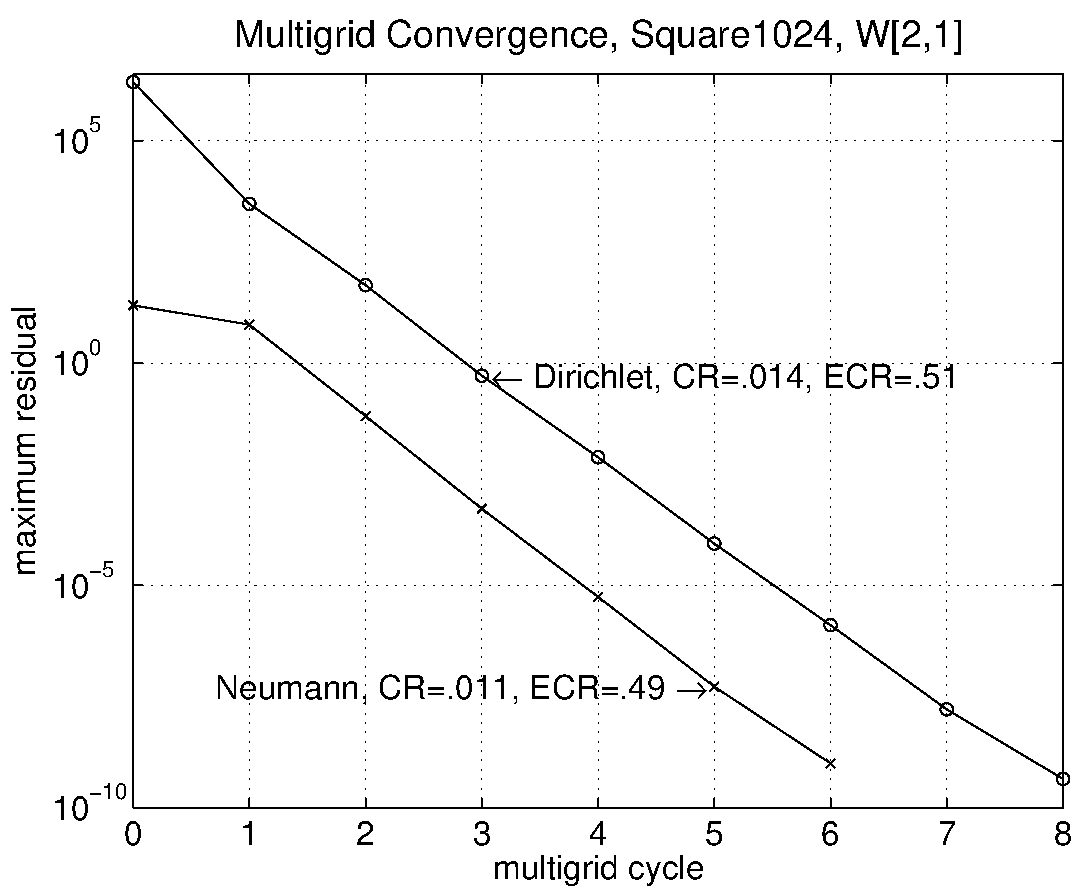
\includegraphics[width=.32\linewidth]{fig/residual_square1024_DN}
  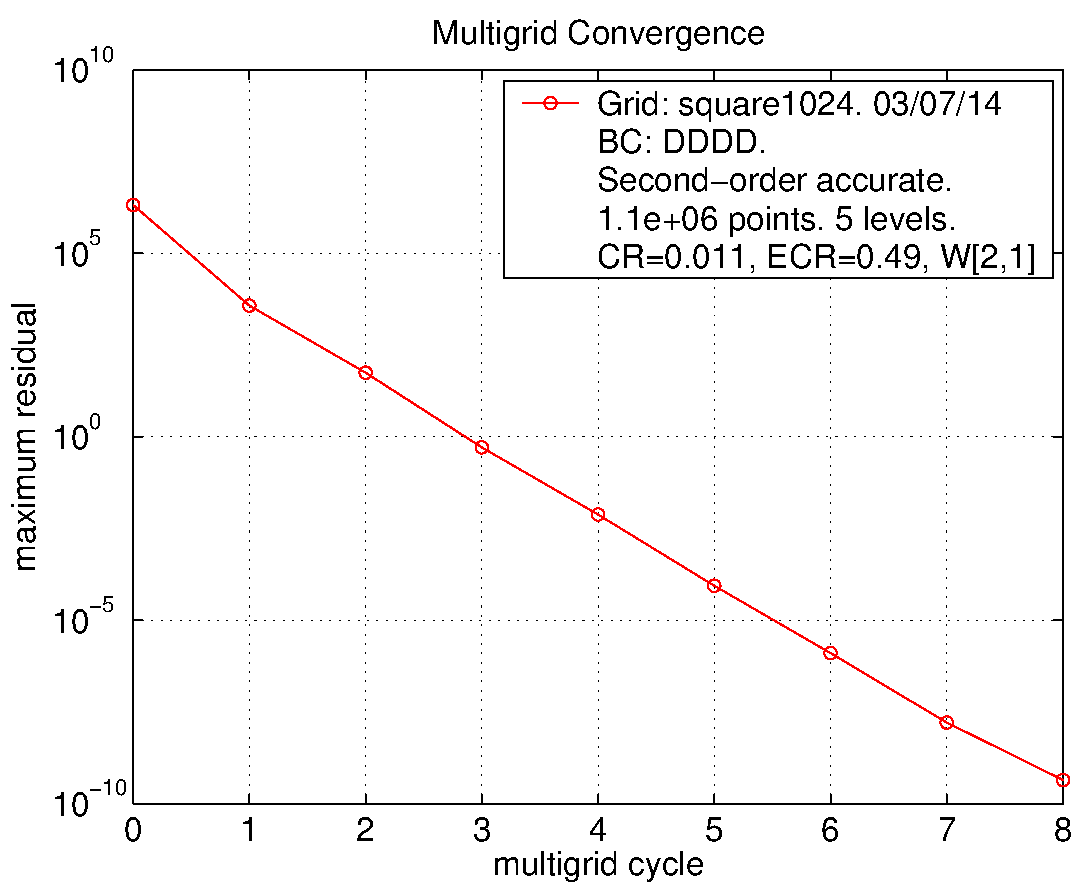
\includegraphics[width=.32\linewidth]{fig/residual_square1024}
  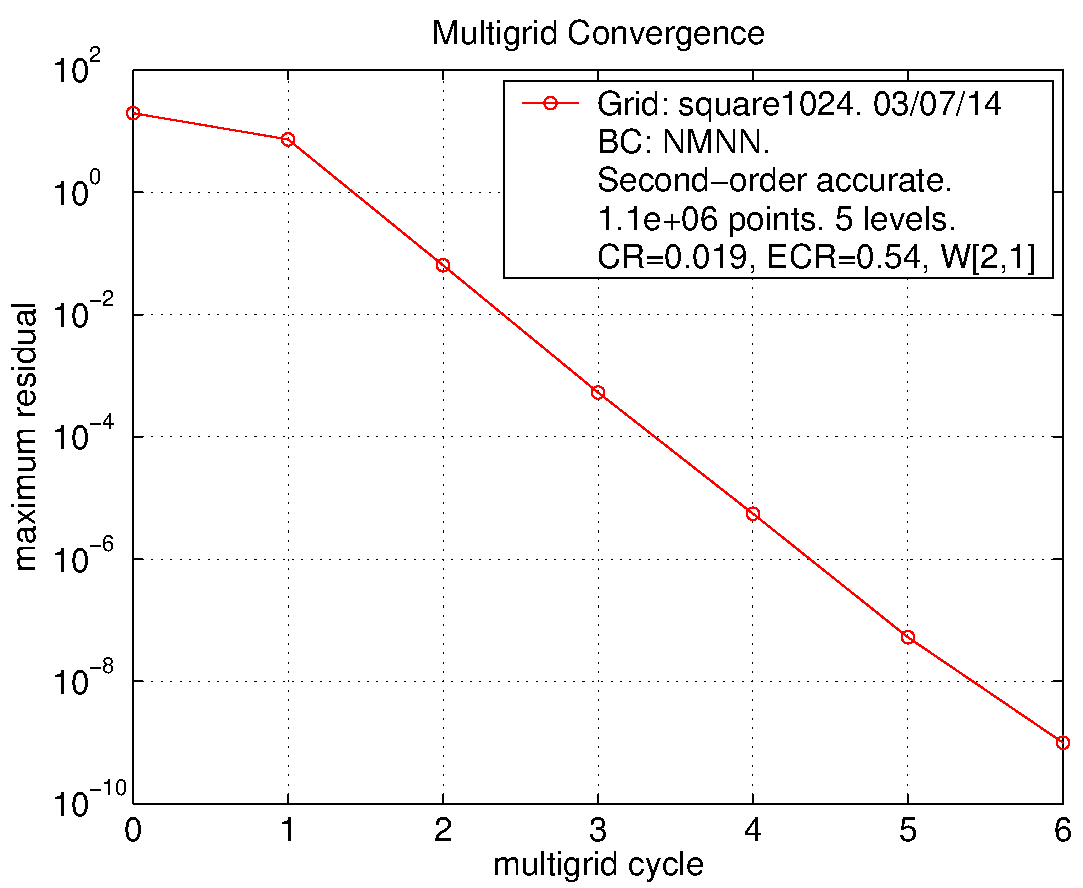
\includegraphics[width=.32\linewidth]{fig/residual_square1024_mixed}
  \end{center} 
\caption{Convergence history for square1024, second-order accuracy. A comparison between Dirichlet
boundary conditions and Neumann/mixed boundary conditions.}
\label{fig:square1024}
\end{figure}


%- \begin{figure}
%- \begin{center}
%- 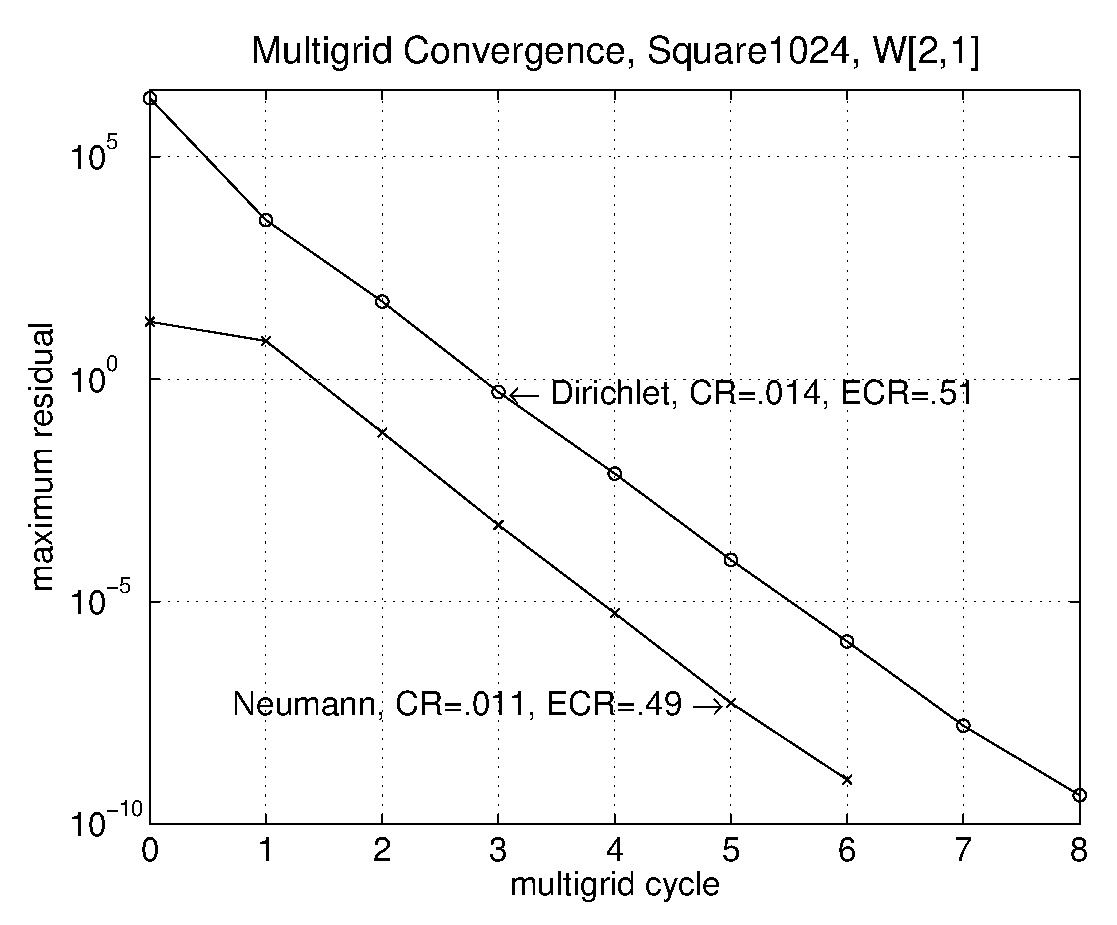
\epsfig{file=residual.square1024.DN.eps,width=\figWidth}
%- 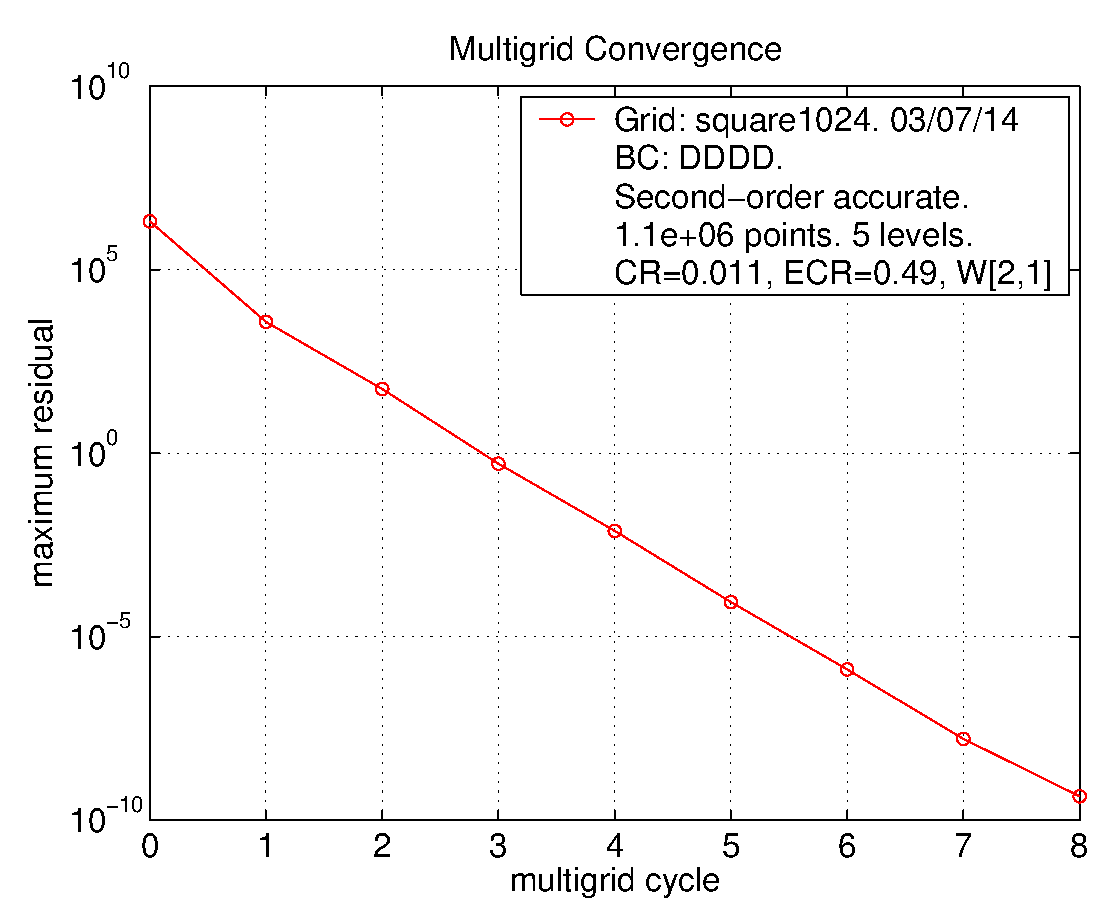
\epsfig{file=residual.square1024.eps,width=\figWidth}
%- 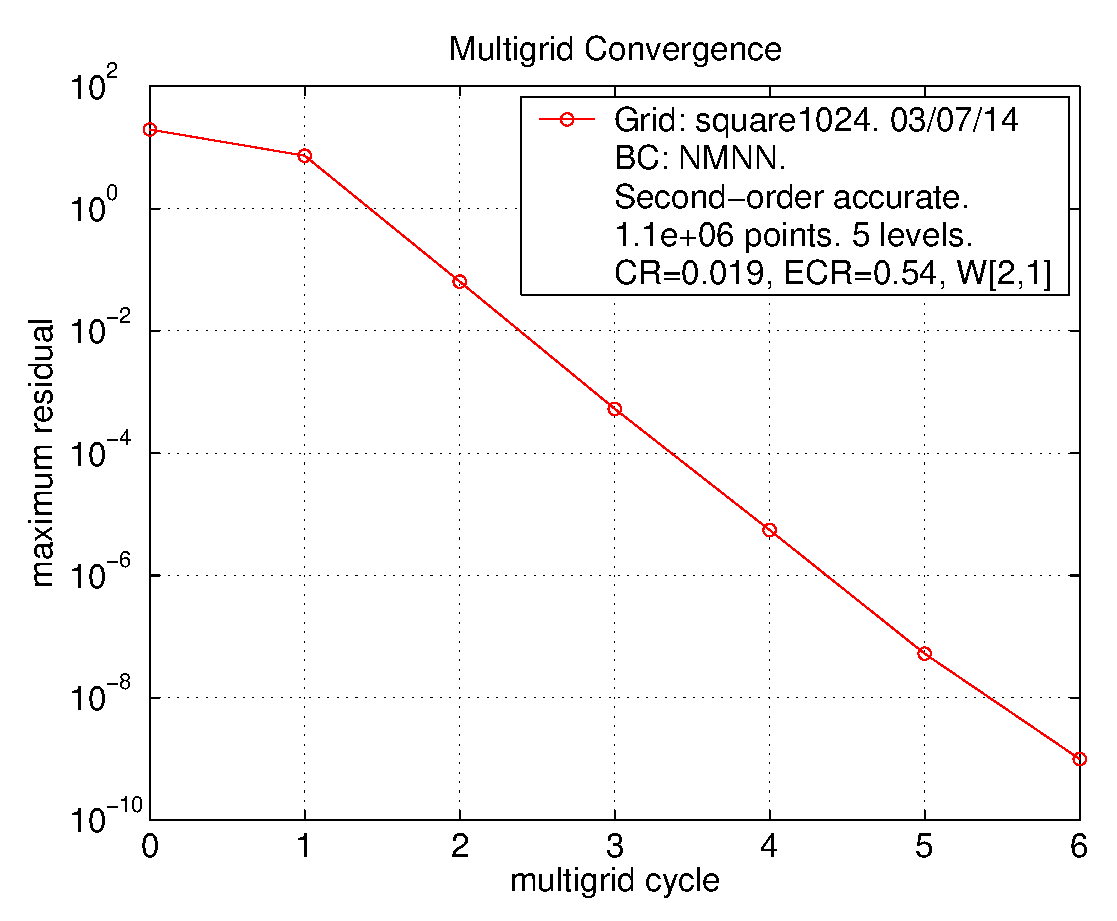
\epsfig{file=residual.square1024.mixed.eps,width=\figWidth}
%- \end{center}
%- \caption{Convergence history for square1024, second-order accuracy. A comparison between Dirichlet
%- boundary conditions and Neumann/mixed boundary conditions.}
%- \label{fig:square1024}
%- \end{figure}

\newcommand{\muLoc}{\mu_{\rm loc}}
\newcommand{\rhoLoc}{\rho_{\rm loc}}
\newcommand{\rhoLocTwoGrid}{\rhoLoc^{(2G)}}
\newcommand{\rhoLocThreeGrid}{\rhoLoc^{(3G)}}

Recall that local Fourier analysis (LFA) can be used to determine 
\begin{align*}
  \muLoc &=  \mbox{smoothing factor} \\
  \rhoLocTwoGrid &= \mbox{asymptotic two-grid convergence factor} \\ 
  \rhoLocThreeGrid &= \mbox{asymptotic three-grid convergence factor} 
\end{align*}

Table~(\ref{tab:ratesSecondOrder2D}) shows the smoothing factor,
two grid and three grid asymptotic convergence rates, as computed by local Fourier analysis, LFA,
for a standard 5-point operator. In the last two columns we show the numerical computed convergence
rate (average) for V and W cycles on a $1024^2$ square.
In general, one might expect the two-grid convergence factor to reflect the results of a W-cycle
while the three-grid convergence factor should be more like the V-cycle.

% For comparison the smoothing factor,
% two grid and three grid asymptotic convergence rates, as computed by local Fourier analysis, LFA,
% for a standard 5-point operator are
% \begin{align*}
%    \muLoc &= .0335 \\
%    \rhoLocTwoGrid(W[2,1]) &= .0523 \\
%    \rhoLocThreeGrid(V[2,1]) &= .0737
% \end{align*}
% These are results are for $\nu_1=2$ pre-smooths and $\nu_2=1$ post-smooths.
% The two-grid results should reflect the results of a W-cycle while the three-grid results
% should be more like the V-cycle.
% When the coarse grid operator is generated from a Galerkin approach the convergence rate is
% \begin{align*}
%    \muLoc &= .0335 \\
%    \rhoLocTwoGrid(W[2,1]) &=  .0284 \\
%    \rhoLocThreeGrid(V[2,1]) &=  .040 
% \end{align*}
% When the relaxation paramter is chosen as $\omega=1.10$ then the smoothing rate is worse
% but the asymptotic convergence factors are much better
% \begin{align*}
%    \muLoc &= .0440 \\
%    \rhoLocTwoGrid(W[2,1]) &=  .0157 \\
%    \rhoLocThreeGrid(V[2,1]) &=  .0240 
% \end{align*}

The two-grid convergence factor $\rhoLocTwoGrid([2,1]) =  .0157$
for $[\nu_1,\nu_2]=[2,1]$ with  Galerkin averaging 
should be compared to the value of about $.016$ actually obtained on a $1024^2$ square.
Some of the computation results are given in table~(\ref{fig:squareSecondOrder2D}).
Notice that the computed convergence rate for the $V[2,1]$ cycle starts near $.016$ ($\approx \rhoLocTwoGrid$)
but ends at $.024$ ($\approx \rhoLocThreeGrid$) for the last two cycles. 

We see that the convergence rate for the {\em standard} V[2,1] cycle
of $\rhoLocTwoGrid(W[2,1]) = .0523$ can be improved substantially to 
$\rhoLocTwoGrid(W[2,1])= .0157$ with little extra work.

\begin{table}[hbt]
\begin{center}
\begin{tabular}{|c|c|c|c|c|c|c|c|} \hline 
% \multicolumn{3}{|c|}{} & \multicolumn{3}{|c|}{LFA}  \\ \hline
\multicolumn{3}{|c|}{$\omega$-RB-GS} & \multicolumn{3}{|c|}{LFA} & \multicolumn{2}{|c|}{Computed}  \\ \hline
% \multicolumn{8}{|c|}{}\multicolumn{3}{|c|}{LFA}\multicolumn{2}{|c|}{Computed}  \\ \hline
 $[\nu_1,\nu_2]$ & Galerkin &$\omega$&$\muLoc$ &$\rhoLocTwoGrid$&$\rhoLocThreeGrid$ &$\rho(W)$     &$\rho(V)$\\ \hline\hline
%                &          &        &         &                &                   &              &        \\ \hline
 $[1,1]$         & No       &   $1$  & $.0625$ & $.074$         & $.104$            & $.061$       & $.092$ \\ 
 $[1,1]$         & Yes      &   $1$  & $.0625$ & $.0625$        & $.066$            & $.059$       & $.058$ \\ 
 $[1,1]$         & Yes      & $1.10$ & $.0734$ & \fbox{$.0388$} & $.052$            & \fbox{$.034$}& $.037$ \\ \hline 
 $[2,1]$         & No       &   $1$  & $.0335$ & $.0523$        & $.074$            & $.044$       & $.064$ \\ 
 $[2,1]$         & Yes      &   $1$  & $.0335$ & $.0284$        & $.040$            & $.026$       & $.034$ \\ 
 $[2,1]$         & Yes      & $1.10$ & $.0440$ & \fbox{$.0157$} & $.024$            &\fbox{$.014$} & $.015$ \\ 
\hline \hline
\multicolumn{8}{|c|}{Second-order accuracy, two-dimensional, 5 point Laplacian.}  \\
\hline 
\end{tabular}
\end{center}
\caption{Smoothing rates and asymptotic convergence factors for various $\omega$-RB-GS cycles compared to the computed
convergence rates for a $1024^2$ square.}
\label{tab:ratesSecondOrder2D} 
\end{table}

\newcommand{\ul}{\underline}
Results for the fourth-order accurate case are given in table~(\ref{tab:ratesFourthOrder2D}).
In this case the LFA determined two grid rate $\rhoLocTwoGrid[2,1]\approx .021$ for $\omega=1.15$, 
should be compared to the numerical computed rate of $CR=.018$.
We see that the convergence rate for the {\em standard} V[2,1] cycle
of $\rhoLocTwoGrid([2,1]) = .0927$ can be improved by a factor of about $4.4$ to 
$\rhoLocTwoGrid([2,1])= .0210$ with little extra work.
\begin{table}[hbt]
\begin{center}
\begin{tabular}{|c|c|c|c|c|c|c|c|} \hline 
% \multicolumn{3}{|c|}{} & \multicolumn{3}{|c|}{LFA}  \\ \hline
\multicolumn{3}{|c|}{$\omega$-RB-GS} & \multicolumn{3}{|c|}{LFA} & \multicolumn{2}{|c|}{Computed}  \\ \hline
% \multicolumn{8}{|c|}{}\multicolumn{3}{|c|}{LFA}\multicolumn{2}{|c|}{Computed}  \\ \hline
 $[\nu_1,\nu_2]$ & Galerkin &$\omega$&$\muLoc$ &$\rhoLocTwoGrid$&$\rhoLocThreeGrid$ &$\rho(W)$    &$\rho(V)$\\ \hline\hline 
 $[1,1]$         & No       &   $1$  & $.0809$ & $.126$         & $.178$            &             &        \\ 
 $[1,1]$         & Yes      &   $1$  & $.0809$ & $.0809$        & $.089$            &             &        \\ \hline
 $[2,1]$         & No       &   $1$  & $.0346$ & $.0927$        & $.128$            & $.082$      & $.128$ \\ 
 $[2,1]$         & Yes      &   $1$  & $.0346$ & $.0516$        & $.060$            & $.048$      & $.054$  \\ 
 $[2,1]$         & Yes      & $1.15$ & $.0530$ & \fbox{$.0210$} & $.030$            &\fbox{$.015$}& $.015$ \\ 
\hline \hline
\multicolumn{8}{|c|}{Fourth-order accuracy, two-dimensional, 9 point Laplacian.}  \\
\hline 
\end{tabular}
\end{center}
\caption{Smoothing rates and asymptotic convergence factors for various $\omega$-RB-GS cycles compared to the computed
convergence rates for a $1024^2$ square.}
\label{tab:ratesFourthOrder2D} 
\end{table}

\begin{figure}[hbt]
\begin{center}
  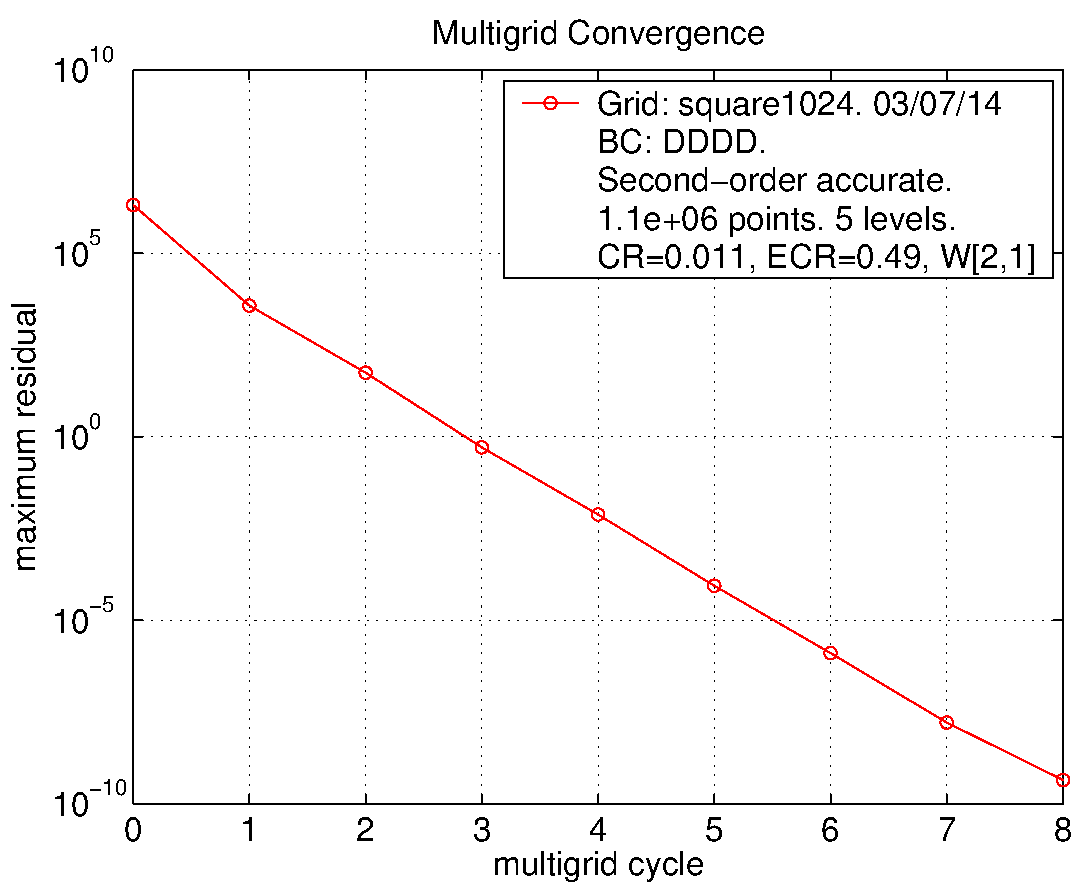
\includegraphics[width=.475\linewidth]{fig/residual_square1024}
  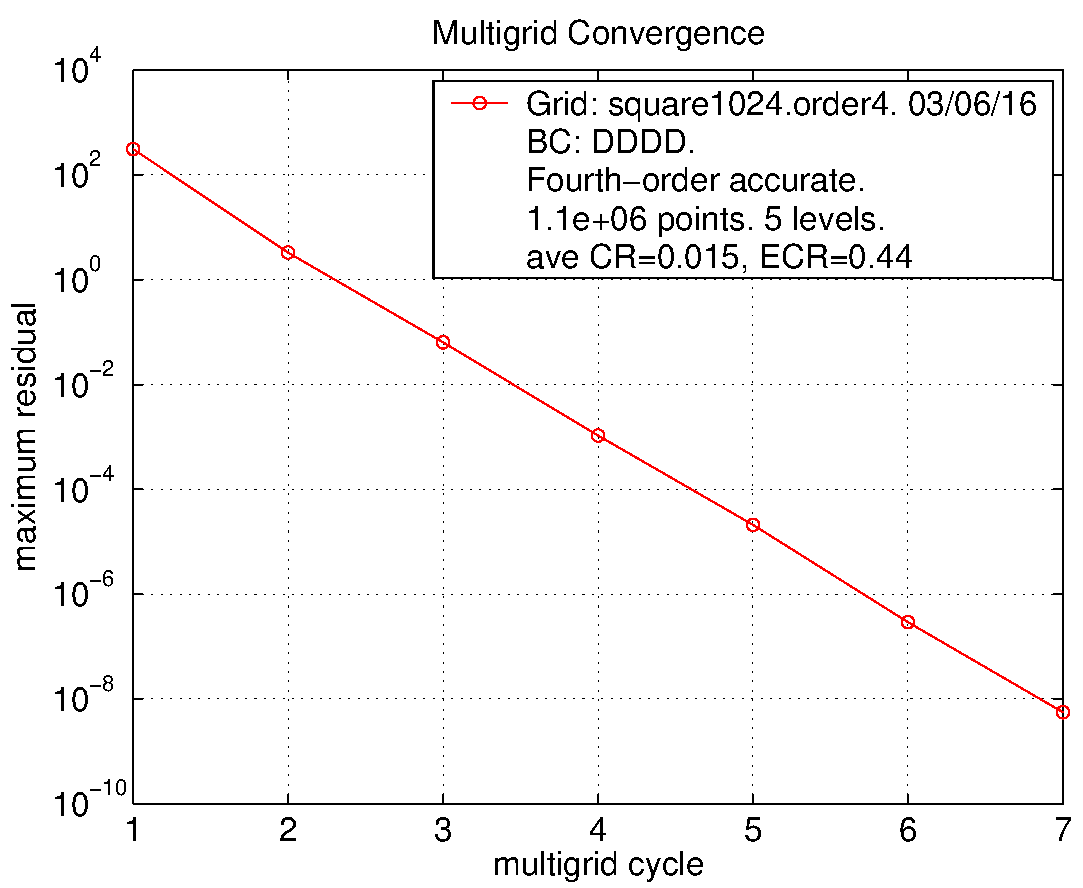
\includegraphics[width=.475\linewidth]{fig/residual_square1024_order4}
  \end{center} 
\caption{Convergence history for square1024, second- and fourth-order accuracy, V(2,1) cycle.
The convergence rate for the fourth-order accurate discretization is almost as good as the second-order accurate case.
% Average convergence rate was CR=.015, and the average effective convergence rate was ECR=.44
}
\label{fig:square1024}
\end{figure}



%- 
%- 
%- \renewcommand{\figWidth}{.495\linewidth}
%- 
%- \begin{figure}
%- \begin{center}
%- 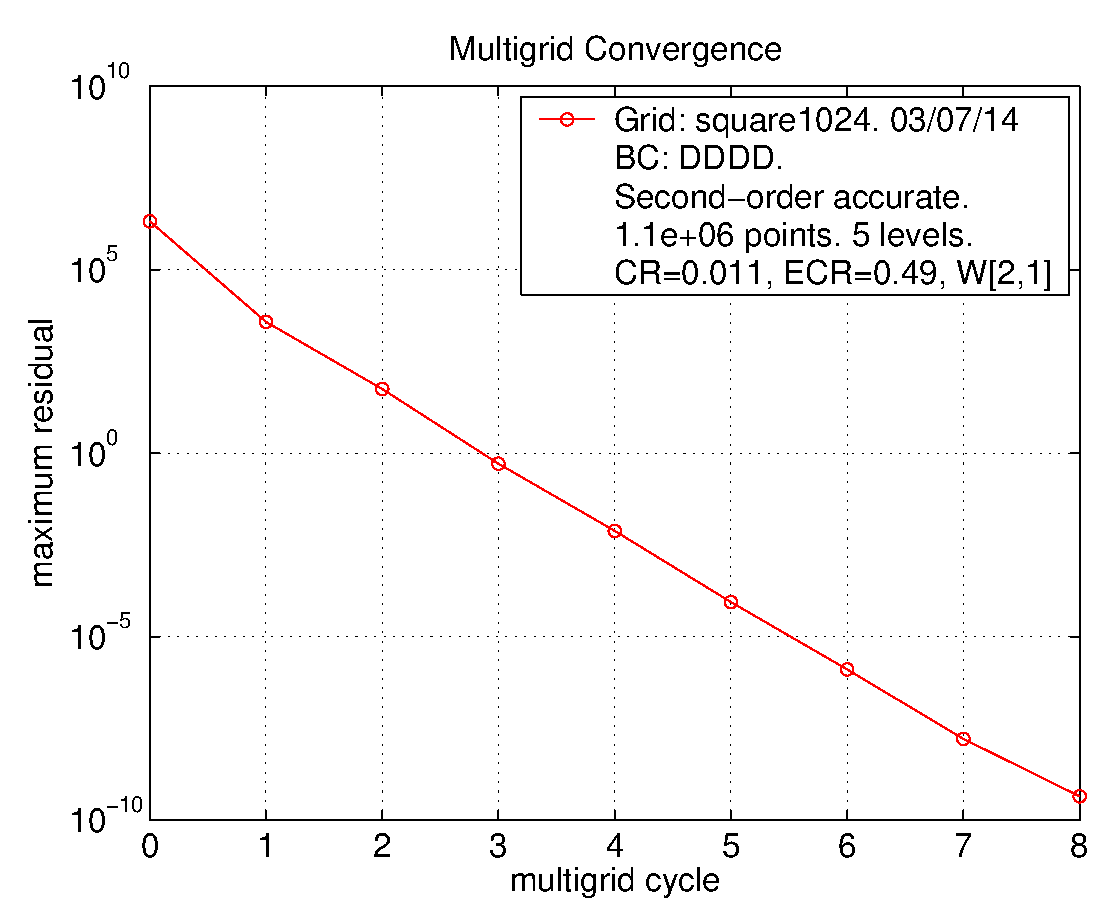
\epsfig{file=residual.square1024.eps,width=\figWidth}
%- 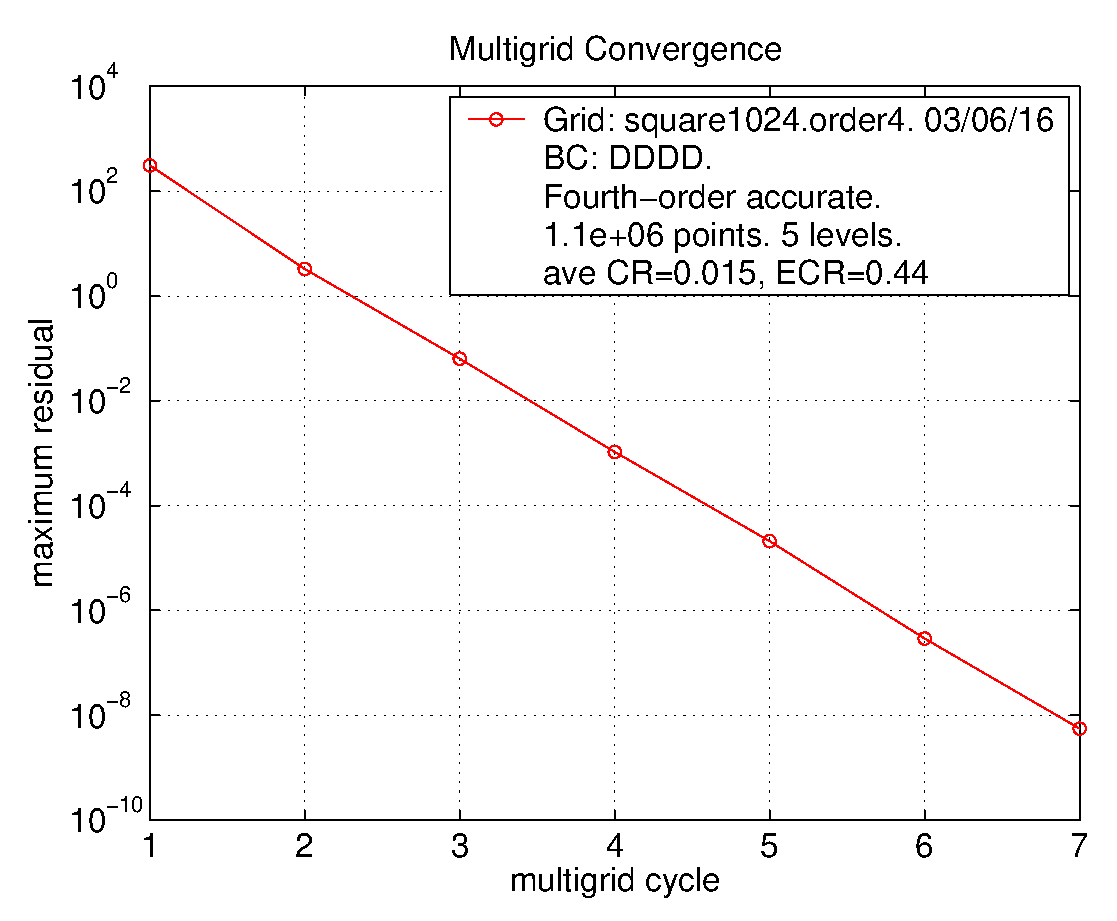
\epsfig{file=residual.square1024.order4.eps,width=\figWidth}
%- \end{center}
%- \caption{Convergence history for square1024, second- and fourth-order accuracy, V(2,1) cycle.
%- The convergence rate for the fourth-order accurate discretization is almost as good as the second-order accurate case.
%- % Average convergence rate was CR=.015, and the average effective convergence rate was ECR=.44
%- }
%- \label{fig:square1024}
%- \end{figure}

\renewcommand{\tablefontsize}{\footnotesize}
% =======================================================================================================
\clearpage
\subsubsection{Second-order accuracy}
% =======================================================================================================

\begin{table}[hbt]
\begin{center}
{\tablefontsize
\begin{tabular}{|c|c|c|c|c|} \hline 
 $i$   & $\vert\vert\mbox{res}\vert\vert_\infty$  &  CR     &  WU    & ECR  \\   \hline 
 $ 1$  & $ 1.2e-01$ & $0.017$ & $ 5.1$ & $0.45$ \\ 
 $ 2$  & $ 1.9e-03$ & $0.016$ & $ 5.1$ & $0.45$ \\ 
 $ 3$  & $ 3.2e-05$ & $0.017$ & $ 5.1$ & $0.45$ \\ 
 $ 4$  & $ 5.3e-07$ & $0.017$ & $ 5.1$ & $0.45$ \\ 
 $ 5$  & $ 8.6e-09$ & $0.016$ & $ 5.1$ & $0.45$ \\ 
 $ 6$  & $ 1.3e-10$ & $0.015$ & $ 5.1$ & $0.44$ \\ 
 $ 7$  & $ 2.2e-12$ & $0.017$ & $ 5.1$ & $0.45$ \\ 
\hline 
\multicolumn{5}{|c|}{Grid: square32. 03/06/12}  \\
\multicolumn{5}{|c|}{BC: DDDD.}  \\
\multicolumn{5}{|c|}{Second-order accurate.}  \\
\multicolumn{5}{|c|}{Trigonometric solution.}  \\
\multicolumn{5}{|c|}{V[2,1]: rb $\omega=1.10$}  \\
\multicolumn{5}{|c|}{1.37e+03 grid-points. 5 levels.}  \\
\multicolumn{5}{|c|}{Average CR=$0.016$, ECR=$0.45$.}  \\
\multicolumn{5}{|c|}{time/cycle = 1.35e-02 s.}  \\
\hline 
\end{tabular}
% \qquad % --------------------------------------------------------------------
\begin{tabular}{|c|c|c|c|c|} \hline 
 $i$   & $\vert\vert\mbox{res}\vert\vert_\infty$  &  CR     &  WU    & ECR  \\   \hline 
 $ 1$  & $ 2.2e+02$ & $0.015$ & $ 5.0$ & $0.43$ \\ 
 $ 2$  & $ 3.5e+00$ & $0.016$ & $ 5.0$ & $0.44$ \\ 
 $ 3$  & $ 5.4e-02$ & $0.016$ & $ 5.0$ & $0.44$ \\ 
 $ 4$  & $ 8.4e-04$ & $0.015$ & $ 5.0$ & $0.44$ \\ 
 $ 5$  & $ 1.3e-05$ & $0.015$ & $ 5.0$ & $0.44$ \\ 
 $ 6$  & $ 2.0e-07$ & $0.015$ & $ 5.0$ & $0.44$ \\ 
 $ 7$  & $ 3.1e-09$ & $0.015$ & $ 5.0$ & $0.44$ \\ 
\hline 
\multicolumn{5}{|c|}{Grid: square1024. 03/06/15}  \\
\multicolumn{5}{|c|}{BC: DDDD.}  \\
\multicolumn{5}{|c|}{Second-order accurate.}  \\
\multicolumn{5}{|c|}{Trigonometric solution.}  \\
\multicolumn{5}{|c|}{V[2,1]: ALT-rb $\omega=1.10$}  \\
\multicolumn{5}{|c|}{1.06e+06 grid-points. 5 levels.}  \\
\multicolumn{5}{|c|}{Average CR=$0.015$, ECR=$0.44$.}  \\
\multicolumn{5}{|c|}{time/cycle = 6.24e-01 s.}  \\
\hline 
\end{tabular}
\begin{tabular}{|c|c|c|c|c|} \hline 
 $i$   & $\vert\vert\mbox{res}\vert\vert_\infty$  &  CR     &  WU    & ECR  \\   \hline 
 $ 1$  & $ 1.0e+02$ & $0.016$ & $ 5.0$ & $0.44$ \\ 
 $ 2$  & $ 1.6e+00$ & $0.016$ & $ 5.0$ & $0.44$ \\ 
 $ 3$  & $ 2.5e-02$ & $0.016$ & $ 5.0$ & $0.44$ \\ 
 $ 4$  & $ 3.9e-04$ & $0.015$ & $ 5.0$ & $0.44$ \\ 
 $ 5$  & $ 6.0e-06$ & $0.015$ & $ 5.0$ & $0.44$ \\ 
 $ 6$  & $ 1.5e-07$ & $0.025$ & $ 5.0$ & $0.48$ \\ 
 $ 7$  & $ 3.5e-09$ & $0.024$ & $ 5.0$ & $0.48$ \\ 
\hline 
\multicolumn{5}{|c|}{Grid: square1024. 03/06/12}  \\
\multicolumn{5}{|c|}{BC: DDDD.}  \\
\multicolumn{5}{|c|}{Second-order accurate.}  \\
\multicolumn{5}{|c|}{Trigonometric solution.}  \\
\multicolumn{5}{|c|}{V[2,1]: rb $\omega=1.10$}  \\
\multicolumn{5}{|c|}{1.06e+06 grid-points. 5 levels.}  \\
\multicolumn{5}{|c|}{Average CR=$0.018$, ECR=$0.45$.}  \\
\multicolumn{5}{|c|}{time/cycle = 6.30e-01 s.}  \\
\hline 
\end{tabular}
% \begin{tabular}{|c|c|c|c|c|} \hline 
%  $i$   & res      & rate    &  WU    & ECR  \\   \hline 
%  $ 1$  & $ 1.3e+03$ & $0.024$ & $ 5.0$ & $0.48$ \\ 
%  $ 2$  & $ 1.1e+01$ & $0.008$ & $ 5.0$ & $0.38$ \\ 
%  $ 3$  & $ 1.8e-01$ & $0.017$ & $ 5.0$ & $0.44$ \\ 
%  $ 4$  & $ 2.8e-03$ & $0.015$ & $ 5.0$ & $0.44$ \\ 
%  $ 5$  & $ 4.4e-05$ & $0.016$ & $ 5.0$ & $0.44$ \\ 
%  $ 6$  & $ 6.6e-07$ & $0.015$ & $ 5.0$ & $0.43$ \\ 
%  $ 7$  & $ 1.1e-08$ & $0.016$ & $ 5.0$ & $0.44$ \\ 
% \hline 
% \multicolumn{5}{|c|}{Grid: square1024.}  \\
% \multicolumn{5}{|c|}{Dirichlet boundary conditions.}  \\
% \multicolumn{5}{|c|}{Second-order accurate.}  \\
% \multicolumn{5}{|c|}{Trigonometric solution.}  \\
% \multicolumn{5}{|c|}{Smoother rb[2,1] $\omega=1.10$}  \\
% \multicolumn{5}{|c|}{1.06e+06 grid-points. 5 levels.}  \\
% \multicolumn{5}{|c|}{Average CR=$0.015$, ECR=$0.44$.}  \\
% \multicolumn{5}{|c|}{time/cycle = 6.16e-01 s.}  \\
% \hline 
% \end{tabular}
% \qquad % --------------------------------------------------------------------
% \vskip\baselineskip
\begin{tabular}{|c|c|c|c|c|} \hline 
 $i$   & $\vert\vert\mbox{res}\vert\vert_\infty$  &  CR     &  WU    & ECR  \\   \hline 
 $ 1$  & $ 7.7e+02$ & $0.033$ & $ 4.0$ & $0.42$ \\ 
 $ 2$  & $ 3.2e+01$ & $0.042$ & $ 4.0$ & $0.45$ \\ 
 $ 3$  & $ 1.2e+00$ & $0.036$ & $ 4.0$ & $0.43$ \\ 
 $ 4$  & $ 3.7e-02$ & $0.032$ & $ 4.0$ & $0.42$ \\ 
 $ 5$  & $ 1.4e-03$ & $0.037$ & $ 4.0$ & $0.44$ \\ 
 $ 6$  & $ 5.3e-05$ & $0.039$ & $ 4.0$ & $0.44$ \\ 
 $ 7$  & $ 1.9e-06$ & $0.037$ & $ 4.0$ & $0.44$ \\ 
%  $ 8$  & $ 7.0e-08$ & $0.036$ & $ 4.0$ & $0.43$ \\ 
%  $ 9$  & $ 2.7e-09$ & $0.039$ & $ 4.0$ & $0.44$ \\ 
\hline 
\multicolumn{5}{|c|}{Grid: square1024. 03/06/12}  \\
\multicolumn{5}{|c|}{BC: DDDD.}  \\
\multicolumn{5}{|c|}{Second-order accurate.}  \\
\multicolumn{5}{|c|}{Trigonometric solution.}  \\
\multicolumn{5}{|c|}{V[1,1]: rb $\omega=1.10$}  \\
\multicolumn{5}{|c|}{1.06e+06 grid-points. 5 levels.}  \\
\multicolumn{5}{|c|}{Average CR=$0.037$, ECR=$0.43$.}  \\
\multicolumn{5}{|c|}{time/cycle = 5.49e-01 s.}  \\
\hline 
\end{tabular}
\begin{tabular}{|c|c|c|c|c|} \hline 
 $i$   & $\vert\vert\mbox{res}\vert\vert_\infty$  &  CR     &  WU    & ECR  \\   \hline 
 $ 1$  & $ 2.9e+01$ & $0.012$ & $ 6.1$ & $0.48$ \\ 
 $ 2$  & $ 2.9e-01$ & $0.010$ & $ 6.1$ & $0.47$ \\ 
 $ 3$  & $ 3.3e-03$ & $0.011$ & $ 6.1$ & $0.48$ \\ 
 $ 4$  & $ 3.7e-05$ & $0.011$ & $ 6.1$ & $0.48$ \\ 
 $ 5$  & $ 4.2e-07$ & $0.011$ & $ 6.1$ & $0.48$ \\ 
 $ 6$  & $ 4.7e-09$ & $0.011$ & $ 6.1$ & $0.48$ \\ 
\hline 
\multicolumn{5}{|c|}{Grid: square1024. 03/06/12}  \\
\multicolumn{5}{|c|}{BC: DDDD.}  \\
\multicolumn{5}{|c|}{Second-order accurate.}  \\
\multicolumn{5}{|c|}{Trigonometric solution.}  \\
\multicolumn{5}{|c|}{V[2,2]: rb $\omega=1.10$}  \\
\multicolumn{5}{|c|}{1.06e+06 grid-points. 5 levels.}  \\
\multicolumn{5}{|c|}{Average CR=$0.011$, ECR=$0.48$.}  \\
\multicolumn{5}{|c|}{time/cycle = 6.99e-01 s.}  \\
\hline 
\end{tabular}
\begin{tabular}{|c|c|c|c|c|} \hline 
 $i$   & res      & rate    &  WU    & ECR  \\   \hline 
 $ 1$  & $ 2.0e+03$ & $0.026$ & $ 6.6$ & $0.58$ \\ 
 $ 2$  & $ 2.4e+01$ & $0.012$ & $ 6.6$ & $0.51$ \\ 
 $ 3$  & $ 4.2e-01$ & $0.018$ & $ 6.6$ & $0.54$ \\ 
 $ 4$  & $ 6.0e-03$ & $0.014$ & $ 6.6$ & $0.53$ \\ 
 $ 5$  & $ 9.7e-05$ & $0.016$ & $ 6.6$ & $0.54$ \\ 
 $ 6$  & $ 1.5e-06$ & $0.015$ & $ 6.6$ & $0.53$ \\ 
 $ 7$  & $ 2.4e-08$ & $0.016$ & $ 6.6$ & $0.53$ \\ 
\hline 
\multicolumn{5}{|c|}{Grid: square1024.}  \\
\multicolumn{5}{|c|}{Dirichlet boundary conditions.}  \\
\multicolumn{5}{|c|}{Second-order accurate.}  \\
\multicolumn{5}{|c|}{Trigonometric solution.}  \\
\multicolumn{5}{|c|}{Smoother lz1[2,1] $\omega=1.00$}  \\
\multicolumn{5}{|c|}{1.06e+06 grid-points. 5 levels.}  \\
\multicolumn{5}{|c|}{Average CR=$0.016$, ECR=$0.54$.}  \\
\multicolumn{5}{|c|}{time/cycle = 8.43e-01 s.}  \\
\hline 
\end{tabular}
% \qquad % --------------------------------------------------------------------
\begin{tabular}{|c|c|c|c|c|} \hline 
 $i$   & $\vert\vert\mbox{res}\vert\vert_\infty$  &  CR     &  WU    & ECR  \\   \hline 
 $ 1$  & $ 1.0e+02$ & $0.014$ & $ 6.1$ & $0.50$ \\ 
 $ 2$  & $ 1.0e+00$ & $0.010$ & $ 6.1$ & $0.47$ \\ 
 $ 3$  & $ 1.5e-02$ & $0.014$ & $ 6.1$ & $0.50$ \\ 
 $ 4$  & $ 1.8e-04$ & $0.012$ & $ 6.1$ & $0.49$ \\ 
 $ 5$  & $ 2.5e-06$ & $0.014$ & $ 6.1$ & $0.50$ \\ 
 $ 6$  & $ 3.3e-08$ & $0.013$ & $ 6.1$ & $0.49$ \\ 
 $ 7$  & $ 7.5e-10$ & $0.023$ & $ 6.1$ & $0.54$ \\ 
\hline 
\multicolumn{5}{|c|}{Grid: square1024. 03/06/15}  \\
\multicolumn{5}{|c|}{BC: DDDD.}  \\
\multicolumn{5}{|c|}{Second-order accurate.}  \\
\multicolumn{5}{|c|}{Trigonometric solution.}  \\
\multicolumn{5}{|c|}{W[2,1]: ALT-rb $\omega=1.10$}  \\
\multicolumn{5}{|c|}{1.06e+06 grid-points. 5 levels.}  \\
\multicolumn{5}{|c|}{Average CR=$0.014$, ECR=$0.50$.}  \\
\multicolumn{5}{|c|}{time/cycle = 9.00e-01 s.}  \\
\hline 
\end{tabular}
\begin{tabular}{|c|c|c|c|c|} \hline 
 $i$   & $\vert\vert\mbox{res}\vert\vert_\infty$  &  CR     &  WU    & ECR  \\   \hline 
 $ 1$  & $ 5.6e+01$ & $0.015$ & $ 6.1$ & $0.50$ \\ 
 $ 2$  & $ 5.2e-01$ & $0.009$ & $ 6.1$ & $0.46$ \\ 
 $ 3$  & $ 7.6e-03$ & $0.015$ & $ 6.1$ & $0.50$ \\ 
 $ 4$  & $ 8.7e-05$ & $0.011$ & $ 6.1$ & $0.48$ \\ 
 $ 5$  & $ 1.3e-06$ & $0.015$ & $ 6.1$ & $0.50$ \\ 
 $ 6$  & $ 1.6e-08$ & $0.013$ & $ 6.1$ & $0.49$ \\ 
 $ 7$  & $ 4.4e-10$ & $0.027$ & $ 6.1$ & $0.55$ \\ 
\hline 
\multicolumn{5}{|c|}{Grid: square1024. 03/06/12}  \\
\multicolumn{5}{|c|}{BC: DDDD.}  \\
\multicolumn{5}{|c|}{Second-order accurate.}  \\
\multicolumn{5}{|c|}{Trigonometric solution.}  \\
\multicolumn{5}{|c|}{W[2,1]: rb $\omega=1.10$}  \\
\multicolumn{5}{|c|}{1.06e+06 grid-points. 5 levels.}  \\
\multicolumn{5}{|c|}{Average CR=$0.014$, ECR=$0.50$.}  \\
\multicolumn{5}{|c|}{time/cycle = 9.05e-01 s.}  \\
\hline 
\end{tabular}
\begin{tabular}{|c|c|c|c|c|} \hline 
 $i$   & $\vert\vert\mbox{res}\vert\vert_\infty$  &  CR     &  WU    & ECR  \\   \hline 
 $ 1$  & $ 6.5e+03$ & $0.076$ & $ 4.0$ & $0.52$ \\ 
 $ 2$  & $ 5.4e+02$ & $0.082$ & $ 4.0$ & $0.53$ \\ 
 $ 3$  & $ 4.6e+01$ & $0.086$ & $ 4.0$ & $0.54$ \\ 
 $ 4$  & $ 4.5e+00$ & $0.097$ & $ 4.0$ & $0.56$ \\ 
 $ 5$  & $ 4.3e-01$ & $0.097$ & $ 4.0$ & $0.56$ \\ 
 $ 6$  & $ 4.2e-02$ & $0.097$ & $ 4.0$ & $0.56$ \\ 
 $ 7$  & $ 4.1e-03$ & $0.098$ & $ 4.0$ & $0.56$ \\ 
%  $ 8$  & $ 4.1e-04$ & $0.099$ & $ 4.0$ & $0.56$ \\ 
%  $ 9$  & $ 4.0e-05$ & $0.099$ & $ 4.0$ & $0.56$ \\ 
\hline 
\multicolumn{5}{|c|}{Grid: square1024. 03/06/13}  \\
\multicolumn{5}{|c|}{BC: DDDD.}  \\
\multicolumn{5}{|c|}{Second-order accurate.}  \\
\multicolumn{5}{|c|}{Trigonometric solution.}  \\
\multicolumn{5}{|c|}{V[1,1]: rb $\omega=1.00$}  \\
\multicolumn{5}{|c|}{1.06e+06 grid-points. 5 levels.}  \\
\multicolumn{5}{|c|}{Average CR=$0.092$, ECR=$0.55$.}  \\
\multicolumn{5}{|c|}{time/cycle = 5.41e-01 s.}  \\
\hline 
\end{tabular}
} % end \tablefontsize
\end{center}
\caption{Multigrid convergence rates for a square, second-order accuracy. A comparison of various methods and
their convergence rates.ALT-rb : alternate smoothing direction. }
\label{fig:squareSecondOrder2D} 
\end{table}




% *********************************************************************************************************************
\begin{table}[hbt]
\begin{center}
{\tablefontsize
\begin{tabular}{|c|c|c|c|c|} \hline 
 $i$   & $\vert\vert\mbox{res}\vert\vert_\infty$  &  CR     &  WU    & ECR  \\   \hline 
 $ 1$  & $ 1.2e+01$ & $0.007$ & $ 6.1$ & $0.44$ \\ 
 $ 2$  & $ 5.6e-02$ & $0.005$ & $ 6.1$ & $0.42$ \\ 
 $ 3$  & $ 8.3e-04$ & $0.015$ & $ 6.1$ & $0.50$ \\ 
 $ 4$  & $ 5.4e-06$ & $0.007$ & $ 6.1$ & $0.44$ \\ 
 $ 5$  & $ 7.0e-08$ & $0.013$ & $ 6.1$ & $0.49$ \\ 
 $ 6$  & $ 7.7e-10$ & $0.011$ & $ 6.1$ & $0.48$ \\ 
\hline 
\multicolumn{5}{|c|}{Grid: square1024. 03/06/17}  \\
\multicolumn{5}{|c|}{BC: DDDD.}  \\
\multicolumn{5}{|c|}{Second-order accurate.}  \\
\multicolumn{5}{|c|}{Trigonometric solution.}  \\
\multicolumn{5}{|c|}{W[2,1]: rb $\omega=1.10$, BL=3,3}\\
\multicolumn{5}{|c|}{1.06e+06 grid-points. 5 levels.}  \\
\multicolumn{5}{|c|}{Average CR=$0.009$, ECR=$0.46$.}  \\
\multicolumn{5}{|c|}{time/cycle = 9.59e-01 s.}  \\
\hline 
\end{tabular}
\begin{tabular}{|c|c|c|c|c|} \hline 
 $i$   & $\vert\vert\mbox{res}\vert\vert_\infty$  &  CR     &  WU    & ECR  \\   \hline 
 $ 1$  & $ 2.9e+03$ & $0.060$ & $ 5.0$ & $0.57$ \\ 
 $ 2$  & $ 1.7e+02$ & $0.059$ & $ 5.0$ & $0.57$ \\ 
 $ 3$  & $ 1.0e+01$ & $0.060$ & $ 5.0$ & $0.57$ \\ 
 $ 4$  & $ 6.2e-01$ & $0.060$ & $ 5.0$ & $0.57$ \\ 
 $ 5$  & $ 3.7e-02$ & $0.060$ & $ 5.0$ & $0.57$ \\ 
 $ 6$  & $ 2.2e-03$ & $0.060$ & $ 5.0$ & $0.57$ \\ 
 $ 7$  & $ 1.4e-04$ & $0.060$ & $ 5.0$ & $0.57$ \\ 
%  $ 8$  & $ 8.2e-06$ & $0.060$ & $ 5.0$ & $0.57$ \\ 
%  $ 9$  & $ 5.0e-07$ & $0.061$ & $ 5.0$ & $0.57$ \\ 
\hline 
\multicolumn{5}{|c|}{Grid: square1024. 03/06/12}  \\
\multicolumn{5}{|c|}{BC: DDDD.}  \\
\multicolumn{5}{|c|}{Second-order accurate.}  \\
\multicolumn{5}{|c|}{Trigonometric solution.}  \\
\multicolumn{5}{|c|}{V[1,1]: lz1 $\omega=1.00$}  \\
\multicolumn{5}{|c|}{1.06e+06 grid-points. 5 levels.}  \\
\multicolumn{5}{|c|}{Average CR=$0.060$, ECR=$0.57$.}  \\
\multicolumn{5}{|c|}{time/cycle = 7.05e-01 s.}  \\
\hline 
\end{tabular}
\begin{tabular}{|c|c|c|c|c|} \hline 
 $i$   & $\vert\vert\mbox{res}\vert\vert_\infty$  &  CR     &  WU    & ECR  \\   \hline 
 $ 1$  & $ 7.0e+02$ & $0.048$ & $ 8.2$ & $0.69$ \\ 
 $ 2$  & $ 4.2e+01$ & $0.061$ & $ 8.2$ & $0.71$ \\ 
 $ 3$  & $ 2.7e+00$ & $0.063$ & $ 8.2$ & $0.71$ \\ 
 $ 4$  & $ 1.8e-01$ & $0.067$ & $ 8.2$ & $0.72$ \\ 
 $ 5$  & $ 1.3e-02$ & $0.074$ & $ 8.2$ & $0.73$ \\ 
 $ 6$  & $ 9.8e-04$ & $0.074$ & $ 8.2$ & $0.73$ \\ 
 $ 7$  & $ 7.4e-05$ & $0.075$ & $ 8.2$ & $0.73$ \\ 
%  $ 8$  & $ 5.8e-06$ & $0.078$ & $ 8.2$ & $0.73$ \\ 
%  $ 9$  & $ 4.6e-07$ & $0.079$ & $ 8.2$ & $0.73$ \\ 
\hline 
\multicolumn{5}{|c|}{Grid: square1024. 03/06/12}  \\
\multicolumn{5}{|c|}{BC: DDDD.}  \\
\multicolumn{5}{|c|}{Second-order accurate.}  \\
\multicolumn{5}{|c|}{Trigonometric solution.}  \\
\multicolumn{5}{|c|}{V[1,1]: alz $\omega=1.00$}  \\
\multicolumn{5}{|c|}{1.06e+06 grid-points. 5 levels.}  \\
\multicolumn{5}{|c|}{Average CR=$0.068$, ECR=$0.72$.}  \\
\multicolumn{5}{|c|}{time/cycle = 1.08e+00 s.}  \\
\multicolumn{5}{|c|}{non-split-zebra XY(XY)XY(XY)}  \\
\hline 
\end{tabular}
% \begin{tabular}{|c|c|c|c|c|} \hline 
%  $i$   & res      & rate    &  WU    & ECR  \\   \hline 
%  $ 1$  & $ 1.2e+03$ & $0.047$ & $ 8.2$ & $0.69$ \\ 
%  $ 2$  & $ 5.9e+01$ & $0.050$ & $ 8.2$ & $0.69$ \\ 
%  $ 3$  & $ 3.6e+00$ & $0.061$ & $ 8.2$ & $0.71$ \\ 
%  $ 4$  & $ 2.3e-01$ & $0.063$ & $ 8.2$ & $0.71$ \\ 
%  $ 5$  & $ 1.5e-02$ & $0.067$ & $ 8.2$ & $0.72$ \\ 
%  $ 6$  & $ 1.1e-03$ & $0.074$ & $ 8.2$ & $0.73$ \\ 
%  $ 7$  & $ 8.5e-05$ & $0.075$ & $ 8.2$ & $0.73$ \\ 
% \hline 
% \multicolumn{5}{|c|}{Grid: square1024.}  \\
% \multicolumn{5}{|c|}{Dirichlet boundary conditions.}  \\
% \multicolumn{5}{|c|}{Second-order accurate.}  \\
% \multicolumn{5}{|c|}{Trigonometric solution.}  \\
% \multicolumn{5}{|c|}{Smoother alz[1,1] $\omega=1.00$}  \\
% \multicolumn{5}{|c|}{1.06e+06 grid-points. 5 levels.}  \\
% \multicolumn{5}{|c|}{Average CR=$0.061$, ECR=$0.71$.}  \\
% \multicolumn{5}{|c|}{time/cycle = 1.08e+00 s.}  \\
% \hline 
% \end{tabular}
\begin{tabular}{|c|c|c|c|c|} \hline 
 $i$   & $\vert\vert\mbox{res}\vert\vert_\infty$  &  CR     &  WU    & ECR  \\   \hline 
 $ 1$  & $ 2.8e+01$ & $0.002$ & $ 8.2$ & $0.47$ \\ 
 $ 2$  & $ 4.8e-01$ & $0.017$ & $ 8.2$ & $0.61$ \\ 
 $ 3$  & $ 3.6e-03$ & $0.008$ & $ 8.2$ & $0.55$ \\ 
 $ 4$  & $ 1.1e-04$ & $0.029$ & $ 8.2$ & $0.65$ \\ 
 $ 5$  & $ 1.6e-06$ & $0.015$ & $ 8.2$ & $0.60$ \\ 
 $ 6$  & $ 4.5e-08$ & $0.028$ & $ 8.2$ & $0.65$ \\ 
 $ 7$  & $ 1.3e-09$ & $0.028$ & $ 8.2$ & $0.65$ \\ 
\hline 
\multicolumn{5}{|c|}{Grid: square1024. 03/06/12}  \\
\multicolumn{5}{|c|}{BC: DDDD.}  \\
\multicolumn{5}{|c|}{Second-order accurate.}  \\
\multicolumn{5}{|c|}{Trigonometric solution.}  \\
\multicolumn{5}{|c|}{V[1,1]: alz $\omega=1.00$}  \\
\multicolumn{5}{|c|}{1.06e+06 grid-points. 5 levels.}  \\
\multicolumn{5}{|c|}{Average CR=$0.014$, ECR=$0.59$.}  \\
\multicolumn{5}{|c|}{time/cycle = 1.10e+00 s.}  \\
\multicolumn{5}{|c|}{variable-alt-zebra: XY(YX)XY(YX)}  \\
\hline 
\end{tabular}
% \begin{tabular}{|c|c|c|c|c|} \hline 
%  $i$   & res      & rate    &  WU    & ECR  \\   \hline 
%  $ 1$  & $ 1.4e+02$ & $0.005$ & $ 8.2$ & $0.53$ \\ 
%  $ 2$  & $ 1.9e+00$ & $0.014$ & $ 8.2$ & $0.59$ \\ 
%  $ 3$  & $ 4.4e-03$ & $0.002$ & $ 8.2$ & $0.48$ \\ 
%  $ 4$  & $ 1.4e-04$ & $0.032$ & $ 8.2$ & $0.66$ \\ 
%  $ 5$  & $ 1.7e-06$ & $0.012$ & $ 8.2$ & $0.58$ \\ 
%  $ 6$  & $ 4.9e-08$ & $0.028$ & $ 8.2$ & $0.65$ \\ 
%  $ 7$  & $ 1.5e-09$ & $0.031$ & $ 8.2$ & $0.65$ \\ 
% \hline 
% \multicolumn{5}{|c|}{Grid: square1024.}  \\
% \multicolumn{5}{|c|}{BC: DDDD.}  \\
% \multicolumn{5}{|c|}{Second-order accurate.}  \\
% \multicolumn{5}{|c|}{Trigonometric solution.}  \\
% \multicolumn{5}{|c|}{Smoother alz-V[1,1] $\omega=1.00$}  \\
% \multicolumn{5}{|c|}{1.06e+06 grid-points. 5 levels.}  \\
% \multicolumn{5}{|c|}{Average CR=$0.013$, ECR=$0.59$.}  \\
% \multicolumn{5}{|c|}{time/cycle = 1.10e+00 s.}  \\
% \multicolumn{5}{|c|}{variable-alt-zebra: XY(YX)XY(YX)}  \\
% \hline 
% \end{tabular}
% \qquad % --------------------------------------------------------------------
\begin{tabular}{|c|c|c|c|c|} \hline 
 $i$   & $\vert\vert\mbox{res}\vert\vert_\infty$  &  CR     &  WU    & ECR  \\   \hline 
 $ 1$  & $ 2.5e+03$ & $0.050$ & $ 5.4$ & $0.57$ \\ 
 $ 2$  & $ 1.0e+01$ & $0.004$ & $ 5.0$ & $0.33$ \\ 
 $ 3$  & $ 9.6e-01$ & $0.095$ & $ 5.0$ & $0.63$ \\ 
 $ 4$  & $ 4.0e-03$ & $0.004$ & $ 5.0$ & $0.33$ \\ 
 $ 5$  & $ 3.7e-04$ & $0.092$ & $ 5.0$ & $0.62$ \\ 
 $ 6$  & $ 2.2e-06$ & $0.006$ & $ 5.0$ & $0.36$ \\ 
 $ 7$  & $ 2.0e-07$ & $0.088$ & $ 5.0$ & $0.62$ \\ 
%  $ 8$  & $ 2.1e-09$ & $0.010$ & $ 5.0$ & $0.40$ \\ 
\hline 
\multicolumn{5}{|c|}{Grid: square1024. 03/06/12}  \\
\multicolumn{5}{|c|}{BC: DDDD.}  \\
\multicolumn{5}{|c|}{Second-order accurate.}  \\
\multicolumn{5}{|c|}{Trigonometric solution.}  \\
\multicolumn{5}{|c|}{V[1,1]: alz $\omega=1.00$}  \\
\multicolumn{5}{|c|}{1.06e+06 grid-points. 5 levels.}  \\
\multicolumn{5}{|c|}{Average CR=$0.021$, ECR=$0.47$.}  \\
\multicolumn{5}{|c|}{time/cycle = 7.59e-01 s.}  \\
\multicolumn{5}{|c|}{variable-zebra: X(Y)X(Y)}  \\
\hline 
\end{tabular}
\begin{tabular}{|c|c|c|c|c|} \hline 
 $i$   & $\vert\vert\mbox{res}\vert\vert_\infty$  &  CR     &  WU    & ECR  \\   \hline 
 $ 1$  & $ 2.6e+03$ & $0.055$ & $ 4.0$ & $0.48$ \\ 
 $ 2$  & $ 1.5e+02$ & $0.056$ & $ 4.0$ & $0.48$ \\ 
 $ 3$  & $ 8.3e+00$ & $0.057$ & $ 4.0$ & $0.49$ \\ 
 $ 4$  & $ 4.7e-01$ & $0.057$ & $ 4.0$ & $0.49$ \\ 
 $ 5$  & $ 2.7e-02$ & $0.057$ & $ 4.0$ & $0.49$ \\ 
 $ 6$  & $ 1.6e-03$ & $0.058$ & $ 4.0$ & $0.49$ \\ 
 $ 7$  & $ 9.3e-05$ & $0.059$ & $ 4.0$ & $0.49$ \\ 
% $ 8$  & $ 5.5e-06$ & $0.059$ & $ 4.0$ & $0.49$ \\ 
%$ 9$  & $ 3.3e-07$ & $0.060$ & $ 4.0$ & $0.49$ \\ 
\hline 
\multicolumn{5}{|c|}{Grid: square1024. 03/06/13}  \\
\multicolumn{5}{|c|}{BC: DDDD.}  \\
\multicolumn{5}{|c|}{Second-order accurate.}  \\
\multicolumn{5}{|c|}{Trigonometric solution.}  \\
\multicolumn{5}{|c|}{V[1,1]: rb $\omega=1.00$}  \\
\multicolumn{5}{|c|}{1.06e+06 grid-points. 5 levels.}  \\
\multicolumn{5}{|c|}{Average CR=$0.058$, ECR=$0.49$.}  \\
\multicolumn{5}{|c|}{time/cycle = 5.45e-01 s.}  \\
\hline 
\end{tabular}
\begin{tabular}{|c|c|c|c|c|} \hline 
 $i$   & $\vert\vert\mbox{res}\vert\vert_\infty$  &  CR     &  WU    & ECR  \\   \hline 
 $ 1$  & $ 3.5e+02$ & $0.029$ & $ 5.0$ & $0.50$ \\ 
 $ 2$  & $ 1.1e+01$ & $0.030$ & $ 5.0$ & $0.50$ \\ 
 $ 3$  & $ 3.3e-01$ & $0.032$ & $ 5.0$ & $0.50$ \\ 
 $ 4$  & $ 1.1e-02$ & $0.033$ & $ 5.0$ & $0.51$ \\ 
 $ 5$  & $ 3.7e-04$ & $0.034$ & $ 5.0$ & $0.51$ \\ 
 $ 6$  & $ 1.3e-05$ & $0.033$ & $ 5.0$ & $0.51$ \\ 
 $ 7$  & $ 4.2e-07$ & $0.033$ & $ 5.0$ & $0.51$ \\ 
% $ 8$  & $ 1.4e-08$ & $0.033$ & $ 5.0$ & $0.51$ \\ 
% $ 9$  & $ 7.0e-10$ & $0.051$ & $ 5.0$ & $0.55$ \\ 
\hline 
\multicolumn{5}{|c|}{Grid: square1024. 03/06/13}  \\
\multicolumn{5}{|c|}{BC: DDDD.}  \\
\multicolumn{5}{|c|}{Second-order accurate.}  \\
\multicolumn{5}{|c|}{Trigonometric solution.}  \\
\multicolumn{5}{|c|}{V[2,1]: rb $\omega=1.00$}  \\
\multicolumn{5}{|c|}{1.06e+06 grid-points. 5 levels.}  \\
\multicolumn{5}{|c|}{Average CR=$0.034$, ECR=$0.51$.}  \\
\multicolumn{5}{|c|}{time/cycle = 6.17e-01 s.}  \\
\hline 
\end{tabular}
\begin{tabular}{|c|c|c|c|c|} \hline 
 $i$   & $\vert\vert\mbox{res}\vert\vert_\infty$  &  CR     &  WU    & ECR  \\   \hline 
 $ 1$  & $ 2.4e+02$ & $0.024$ & $ 6.1$ & $0.54$ \\ 
 $ 2$  & $ 5.9e+00$ & $0.025$ & $ 6.1$ & $0.55$ \\ 
 $ 3$  & $ 1.5e-01$ & $0.026$ & $ 6.1$ & $0.55$ \\ 
 $ 4$  & $ 4.0e-03$ & $0.026$ & $ 6.1$ & $0.55$ \\ 
 $ 5$  & $ 1.0e-04$ & $0.026$ & $ 6.1$ & $0.55$ \\ 
 $ 6$  & $ 2.8e-06$ & $0.027$ & $ 6.1$ & $0.55$ \\ 
 $ 7$  & $ 7.4e-08$ & $0.027$ & $ 6.1$ & $0.55$ \\ 
%$ 8$  & $ 2.3e-09$ & $0.031$ & $ 6.1$ & $0.57$ \\ 
\hline 
\multicolumn{5}{|c|}{Grid: square1024. 03/06/13}  \\
\multicolumn{5}{|c|}{BC: DDDD.}  \\
\multicolumn{5}{|c|}{Second-order accurate.}  \\
\multicolumn{5}{|c|}{Trigonometric solution.}  \\
\multicolumn{5}{|c|}{W[2,1]: rb $\omega=1.00$}  \\
\multicolumn{5}{|c|}{1.06e+06 grid-points. 5 levels.}  \\
\multicolumn{5}{|c|}{Average CR=$0.026$, ECR=$0.55$.}  \\
\multicolumn{5}{|c|}{time/cycle = 8.96e-01 s.}  \\
\hline 
\end{tabular}
% \begin{tabular}{|c|c|c|c|c|} \hline 
%  $i$   & res      & rate    &  WU    & ECR  \\   \hline 
%  $ 1$  & $ 1.1e+04$ & $0.054$ & $ 5.4$ & $0.58$ \\ 
%  $ 2$  & $ 6.7e+01$ & $0.006$ & $ 5.0$ & $0.36$ \\ 
%  $ 3$  & $ 4.5e+00$ & $0.068$ & $ 5.0$ & $0.58$ \\ 
%  $ 4$  & $ 3.2e-02$ & $0.007$ & $ 5.0$ & $0.37$ \\ 
%  $ 5$  & $ 1.8e-03$ & $0.057$ & $ 5.0$ & $0.56$ \\ 
%  $ 6$  & $ 2.5e-05$ & $0.014$ & $ 5.0$ & $0.43$ \\ 
%  $ 7$  & $ 8.8e-07$ & $0.035$ & $ 5.0$ & $0.51$ \\ 
% \hline 
% \multicolumn{5}{|c|}{Grid: square1024.}  \\
% \multicolumn{5}{|c|}{BC: DDDD.}  \\
% \multicolumn{5}{|c|}{Second-order accurate.}  \\
% \multicolumn{5}{|c|}{Trigonometric solution.}  \\
% \multicolumn{5}{|c|}{Smoother alz-V[1,1] $\omega=1.00$}  \\
% \multicolumn{5}{|c|}{1.06e+06 grid-points. 5 levels.}  \\
% \multicolumn{5}{|c|}{Average CR=$0.024$, ECR=$0.48$.}  \\
% \multicolumn{5}{|c|}{time/cycle = 7.88e-01 s.}  \\
% \multicolumn{5}{|c|}{variable-zebra: X(Y)X(Y)}  \\
% \hline 
% \end{tabular}
} % end \tablefontsize
\end{center}
\caption{Multigrid convergence rates for a square, second-order accuracy. A comparison of various methods and
their convergence rates. BL=m,n : boundary smoothing with m layers and n iterations.}
% \label{fig:square} 
\end{table}

% *********************************************************************************************************************

% \begin{table}[hbt]
% \begin{center}
% {\tablefontsize
% 
% } % end \tablefontsize
% \end{center}
% \caption{Multigrid convergence rates for a square, second-order accuracy, LINE SOLVERS}
% % \label{fig:square} 
% \end{table}

% *********************************************************************************************************************

\begin{table}[hbt]
\begin{center}
{\tablefontsize
\begin{tabular}{|c|c|c|c|c|} \hline 
 $i$   & res      & rate    &  WU    & ECR  \\   \hline 
 $ 1$  & $ 4.1e-02$ & $0.024$ & $ 5.0$ & $0.48$ \\ 
 $ 2$  & $ 3.5e-04$ & $0.008$ & $ 5.0$ & $0.39$ \\ 
 $ 3$  & $ 5.7e-06$ & $0.017$ & $ 5.0$ & $0.44$ \\ 
 $ 4$  & $ 9.0e-08$ & $0.016$ & $ 5.0$ & $0.44$ \\ 
\hline 
\multicolumn{5}{|c|}{Grid: square1024.}  \\
\multicolumn{5}{|c|}{BC: DDDD.}  \\
\multicolumn{5}{|c|}{Second-order accurate.}  \\
\multicolumn{5}{|c|}{Trigonometric solution.}  \\
\multicolumn{5}{|c|}{Smoother rb-V[2,1] $\omega=1.10$}  \\
\multicolumn{5}{|c|}{1.06e+06 grid-points. 5 levels.}  \\
\multicolumn{5}{|c|}{Average CR=$0.015$, ECR=$0.44$.}  \\
\multicolumn{5}{|c|}{time/cycle = 7.28e-01 s.}  \\
\hline 
\end{tabular}
% \qquad % --------------------------------------------------------------------
\begin{tabular}{|c|c|c|c|c|} \hline 
 $i$   & res      & rate    &  WU    & ECR  \\   \hline 
 $ 1$  & $ 1.2e-02$ & $0.024$ & $ 5.0$ & $0.48$ \\ 
 $ 2$  & $ 9.0e-05$ & $0.007$ & $ 5.0$ & $0.38$ \\ 
 $ 3$  & $ 1.5e-06$ & $0.017$ & $ 5.0$ & $0.44$ \\ 
 $ 4$  & $ 2.3e-08$ & $0.016$ & $ 5.0$ & $0.44$ \\ 
\hline 
\multicolumn{5}{|c|}{Grid: square1024.}  \\
\multicolumn{5}{|c|}{BC: DDDD.}  \\
\multicolumn{5}{|c|}{Second-order accurate.}  \\
\multicolumn{5}{|c|}{Trigonometric solution.}  \\
\multicolumn{5}{|c|}{Smoother rb-V[2,1] $\omega=1.10$}  \\
\multicolumn{5}{|c|}{1.06e+06 grid-points. 5 levels.}  \\
\multicolumn{5}{|c|}{Average CR=$0.015$, ECR=$0.43$.}  \\
\multicolumn{5}{|c|}{time/cycle = 7.43e-01 s.}  \\
\hline 
\end{tabular}
% \qquad % --------------------------------------------------------------------
% \vskip\baselineskip
\begin{tabular}{|c|c|c|c|c|} \hline 
 $i$   & $\vert\vert\mbox{res}\vert\vert_\infty$  &  CR     &  WU    & ECR  \\   \hline 
 $ 1$  & $ 2.1e-04$ & $0.016$ & $ 5.0$ & $0.44$ \\ 
 $ 2$  & $ 3.4e-06$ & $0.016$ & $ 5.0$ & $0.44$ \\ 
 $ 3$  & $ 5.3e-08$ & $0.016$ & $ 5.0$ & $0.44$ \\ 
\hline 
\multicolumn{5}{|c|}{Grid: square2048.}  \\
\multicolumn{5}{|c|}{BC: DDDD.}  \\
\multicolumn{5}{|c|}{Second-order accurate.}  \\
\multicolumn{5}{|c|}{Trigonometric solution.}  \\
\multicolumn{5}{|c|}{Full Multigrid.}  \\
\multicolumn{5}{|c|}{V[2,1]: rb $\omega=1.10$}  \\
\multicolumn{5}{|c|}{4.21e+06 grid-points. 5 levels.}  \\
\multicolumn{5}{|c|}{Average CR=$0.016$, ECR=$0.44$.}  \\
\multicolumn{5}{|c|}{time/cycle = 3.12e+00 s.}  \\
\hline 
\end{tabular}
\qquad % --------------------------------------------------------------------
} % end \tablefontsize
\end{center}
\caption{Multigrid convergence rates for a square, second-order accuracy, full multigrid. 
Top left: linear-interpolation for the FMG prolongation, top middle: quadratic interpolation.}
% \label{fig:square} 
\end{table}



% *********************************************************************************************************************
% =======================================================================================================
\clearpage
\subsubsection{Second-order Neumann and mixed boundary conditions.}
% =======================================================================================================

\begin{table}[hbt]
\begin{center}
{\tablefontsize
\begin{tabular}{|c|c|c|c|c|} \hline 
 $i$   & $\vert\vert\mbox{res}\vert\vert_\infty$  &  CR     &  WU    & ECR  \\   \hline 
 $ 1$  & $ 8.6e+01$ & $0.014$ & $ 5.0$ & $0.43$ \\ 
 $ 2$  & $ 1.2e+00$ & $0.014$ & $ 5.0$ & $0.43$ \\ 
 $ 3$  & $ 1.7e-02$ & $0.015$ & $ 5.0$ & $0.43$ \\ 
 $ 4$  & $ 3.6e-04$ & $0.021$ & $ 5.0$ & $0.46$ \\ 
 $ 5$  & $ 9.9e-06$ & $0.028$ & $ 5.0$ & $0.49$ \\ 
 $ 6$  & $ 2.6e-07$ & $0.026$ & $ 5.0$ & $0.49$ \\ 
 $ 7$  & $ 5.9e-09$ & $0.023$ & $ 5.0$ & $0.47$ \\ 
\hline 
\multicolumn{5}{|c|}{Grid: square1024. 03/06/12}  \\
\multicolumn{5}{|c|}{BC: NDDD.}  \\
\multicolumn{5}{|c|}{Second-order accurate.}  \\
\multicolumn{5}{|c|}{Trigonometric solution.}  \\
\multicolumn{5}{|c|}{V[2,1]: rb $\omega=1.10$}  \\
\multicolumn{5}{|c|}{1.06e+06 grid-points. 5 levels.}  \\
\multicolumn{5}{|c|}{Average CR=$0.019$, ECR=$0.46$.}  \\
\multicolumn{5}{|c|}{time/cycle = 6.02e-01 s.}  \\
\hline 
\end{tabular}
\begin{tabular}{|c|c|c|c|c|} \hline 
 $i$   & $\vert\vert\mbox{res}\vert\vert_\infty$  &  CR     &  WU    & ECR  \\   \hline 
 $ 1$  & $ 5.7e+01$ & $0.017$ & $ 6.1$ & $0.51$ \\ 
 $ 2$  & $ 5.1e-01$ & $0.009$ & $ 6.1$ & $0.46$ \\ 
 $ 3$  & $ 7.8e-03$ & $0.015$ & $ 6.1$ & $0.50$ \\ 
 $ 4$  & $ 8.9e-05$ & $0.011$ & $ 6.1$ & $0.48$ \\ 
 $ 5$  & $ 1.3e-06$ & $0.015$ & $ 6.1$ & $0.50$ \\ 
 $ 6$  & $ 1.7e-08$ & $0.013$ & $ 6.1$ & $0.49$ \\ 
 $ 7$  & $ 5.3e-10$ & $0.032$ & $ 6.1$ & $0.57$ \\ 
\hline 
\multicolumn{5}{|c|}{Grid: square1024. 03/06/12}  \\
\multicolumn{5}{|c|}{BC: NDDD.}  \\
\multicolumn{5}{|c|}{Second-order accurate.}  \\
\multicolumn{5}{|c|}{Trigonometric solution.}  \\
\multicolumn{5}{|c|}{W[2,1]: rb $\omega=1.10$}  \\
\multicolumn{5}{|c|}{1.06e+06 grid-points. 5 levels.}  \\
\multicolumn{5}{|c|}{Average CR=$0.015$, ECR=$0.50$.}  \\
\multicolumn{5}{|c|}{time/cycle = 8.57e-01 s.}  \\
\hline 
\end{tabular}
\begin{tabular}{|c|c|c|c|c|} \hline 
 $i$   & $\vert\vert\mbox{res}\vert\vert_\infty$  &  CR     &  WU    & ECR  \\   \hline 
 $ 1$  & $ 6.4e-02$ & $0.009$ & $ 6.1$ & $0.46$ \\ 
 $ 2$  & $ 5.3e-04$ & $0.008$ & $ 6.1$ & $0.46$ \\ 
 $ 3$  & $ 5.5e-06$ & $0.010$ & $ 6.1$ & $0.47$ \\ 
 $ 4$  & $ 5.3e-08$ & $0.010$ & $ 6.1$ & $0.47$ \\ 
 $ 5$  & $ 9.9e-10$ & $0.019$ & $ 6.1$ & $0.52$ \\ 
\hline 
\multicolumn{5}{|c|}{Grid: square1024. 03/06/12}  \\
\multicolumn{5}{|c|}{BC: NMNN.}  \\
\multicolumn{5}{|c|}{Second-order accurate.}  \\
\multicolumn{5}{|c|}{Trigonometric solution.}  \\
\multicolumn{5}{|c|}{W[2,1]: rb $\omega=1.10$}  \\
\multicolumn{5}{|c|}{1.06e+06 grid-points. 5 levels.}  \\
\multicolumn{5}{|c|}{Average CR=$0.011$, ECR=$0.48$.}  \\
\multicolumn{5}{|c|}{time/cycle = 8.24e-01 s.}  \\
\hline 
\end{tabular}
\begin{tabular}{|c|c|c|c|c|} \hline 
 $i$   & $\vert\vert\mbox{res}\vert\vert_\infty$  &  CR     &  WU    & ECR  \\   \hline 
 $ 1$  & $ 7.0e+01$ & $0.017$ & $ 6.6$ & $0.54$ \\ 
 $ 2$  & $ 1.1e+00$ & $0.015$ & $ 6.6$ & $0.53$ \\ 
 $ 3$  & $ 1.7e-02$ & $0.016$ & $ 6.6$ & $0.53$ \\ 
 $ 4$  & $ 4.0e-04$ & $0.024$ & $ 6.6$ & $0.57$ \\ 
 $ 5$  & $ 7.7e-06$ & $0.019$ & $ 6.6$ & $0.55$ \\ 
 $ 6$  & $ 1.7e-07$ & $0.023$ & $ 6.6$ & $0.56$ \\ 
 $ 7$  & $ 3.9e-09$ & $0.023$ & $ 6.6$ & $0.56$ \\ 
\hline 
\multicolumn{5}{|c|}{Grid: square1024. 03/06/12}  \\
\multicolumn{5}{|c|}{BC: NDDD.}  \\
\multicolumn{5}{|c|}{Second-order accurate.}  \\
\multicolumn{5}{|c|}{Trigonometric solution.}  \\
\multicolumn{5}{|c|}{V[2,1]: lz1 $\omega=1.00$}  \\
\multicolumn{5}{|c|}{1.06e+06 grid-points. 5 levels.}  \\
\multicolumn{5}{|c|}{Average CR=$0.019$, ECR=$0.55$.}  \\
\multicolumn{5}{|c|}{time/cycle = 8.40e-01 s.}  \\
\hline 
\end{tabular}
\begin{tabular}{|c|c|c|c|c|} \hline 
 $i$   & $\vert\vert\mbox{res}\vert\vert_\infty$  &  CR     &  WU    & ECR  \\   \hline 
 $ 1$  & $ 6.8e+01$ & $0.017$ & $ 7.7$ & $0.59$ \\ 
 $ 2$  & $ 9.7e-01$ & $0.014$ & $ 7.7$ & $0.58$ \\ 
 $ 3$  & $ 1.6e-02$ & $0.016$ & $ 7.7$ & $0.59$ \\ 
 $ 4$  & $ 2.4e-04$ & $0.015$ & $ 7.7$ & $0.58$ \\ 
 $ 5$  & $ 3.7e-06$ & $0.016$ & $ 7.7$ & $0.59$ \\ 
 $ 6$  & $ 5.8e-08$ & $0.016$ & $ 7.7$ & $0.58$ \\ 
 $ 7$  & $ 1.4e-09$ & $0.024$ & $ 7.7$ & $0.62$ \\ 
\hline 
\multicolumn{5}{|c|}{Grid: square1024. 03/06/12}  \\
\multicolumn{5}{|c|}{BC: NDDD.}  \\
\multicolumn{5}{|c|}{Second-order accurate.}  \\
\multicolumn{5}{|c|}{Trigonometric solution.}  \\
\multicolumn{5}{|c|}{W[2,1]: lz1 $\omega=1.00$}  \\
\multicolumn{5}{|c|}{1.06e+06 grid-points. 5 levels.}  \\
\multicolumn{5}{|c|}{Average CR=$0.017$, ECR=$0.59$.}  \\
\multicolumn{5}{|c|}{time/cycle = 1.16e+00 s.}  \\
\hline 
\end{tabular}
% \qquad % --------------------------------------------------------------------
% \vskip\baselineskip
% \qquad % --------------------------------------------------------------------
} % end \tablefontsize
\end{center}
\caption{Multigrid convergence rates for a square, Neumann and mixed boundary conditions.
   Boundary conditions: D=Dirichlet, N=Neumann, M=mixed, P=periodic, I=interpolation. }
 \label{tab:sqNeumann} 
\end{table}


% =======================================================================================================
\clearpage
\subsubsection{Fourth-order accuracy}
% =======================================================================================================

\begin{table}[hbt]
\begin{center}
{\tablefontsize
\begin{tabular}{|c|c|c|c|c|} \hline 
 $i$   & $\vert\vert\mbox{res}\vert\vert_\infty$  &  CR     &  WU    & ECR  \\   \hline 
 $ 1$  & $ 3.1e+02$ & $0.011$ & $ 5.0$ & $0.41$ \\ 
 $ 2$  & $ 3.3e+00$ & $0.011$ & $ 5.0$ & $0.41$ \\ 
 $ 3$  & $ 6.4e-02$ & $0.019$ & $ 5.0$ & $0.46$ \\ 
 $ 4$  & $ 1.1e-03$ & $0.017$ & $ 5.0$ & $0.44$ \\ 
 $ 5$  & $ 2.1e-05$ & $0.020$ & $ 5.0$ & $0.46$ \\ 
 $ 6$  & $ 2.9e-07$ & $0.014$ & $ 5.0$ & $0.43$ \\ 
 $ 7$  & $ 5.5e-09$ & $0.019$ & $ 5.0$ & $0.46$ \\ 
\hline 
\multicolumn{5}{|c|}{Grid: square1024.order4. 03/06/15}  \\
\multicolumn{5}{|c|}{BC: DDDD.}  \\
\multicolumn{5}{|c|}{Fourth-order accurate.}  \\
\multicolumn{5}{|c|}{Trigonometric solution.}  \\
\multicolumn{5}{|c|}{V[2,1]: ALT-rb $\omega=1.15$}  \\
\multicolumn{5}{|c|}{1.06e+06 grid-points. 5 levels.}  \\
\multicolumn{5}{|c|}{Average CR=$0.015$, ECR=$0.44$.}  \\
\multicolumn{5}{|c|}{time/cycle = 8.26e-01 s.}  \\
\hline 
\end{tabular}
\begin{tabular}{|c|c|c|c|c|} \hline 
 $i$   & $\vert\vert\mbox{res}\vert\vert_\infty$  &  CR     &  WU    & ECR  \\   \hline 
 $ 1$  & $ 1.2e+02$ & $0.012$ & $ 5.0$ & $0.42$ \\ 
 $ 2$  & $ 2.1e+00$ & $0.017$ & $ 5.0$ & $0.45$ \\ 
 $ 3$  & $ 3.1e-02$ & $0.015$ & $ 5.0$ & $0.44$ \\ 
 $ 4$  & $ 6.0e-04$ & $0.019$ & $ 5.0$ & $0.46$ \\ 
 $ 5$  & $ 1.2e-05$ & $0.020$ & $ 5.0$ & $0.46$ \\ 
 $ 6$  & $ 3.0e-07$ & $0.026$ & $ 5.0$ & $0.48$ \\ 
 $ 7$  & $ 7.4e-09$ & $0.024$ & $ 5.0$ & $0.48$ \\ 
\hline 
\multicolumn{5}{|c|}{Grid: square1024.order4. 03/06/12}  \\
\multicolumn{5}{|c|}{BC: DDDD.}  \\
\multicolumn{5}{|c|}{Fourth-order accurate.}  \\
\multicolumn{5}{|c|}{Trigonometric solution.}  \\
\multicolumn{5}{|c|}{V[2,1]: rb $\omega=1.15$}  \\
\multicolumn{5}{|c|}{1.06e+06 grid-points. 5 levels.}  \\
\multicolumn{5}{|c|}{Average CR=$0.018$, ECR=$0.45$.}  \\
\multicolumn{5}{|c|}{time/cycle = 8.34e-01 s.}  \\
\hline 
\end{tabular}
\begin{tabular}{|c|c|c|c|c|} \hline 
 $i$   & $\vert\vert\mbox{res}\vert\vert_\infty$  &  CR     &  WU    & ECR  \\   \hline 
 $ 1$  & $ 2.1e+02$ & $0.013$ & $ 6.2$ & $0.49$ \\ 
 $ 2$  & $ 2.4e+00$ & $0.012$ & $ 6.2$ & $0.49$ \\ 
 $ 3$  & $ 4.4e-02$ & $0.018$ & $ 6.2$ & $0.52$ \\ 
 $ 4$  & $ 7.2e-04$ & $0.016$ & $ 6.2$ & $0.51$ \\ 
 $ 5$  & $ 1.1e-05$ & $0.016$ & $ 6.2$ & $0.51$ \\ 
 $ 6$  & $ 1.6e-07$ & $0.014$ & $ 6.2$ & $0.50$ \\ 
 $ 7$  & $ 2.7e-09$ & $0.017$ & $ 6.2$ & $0.52$ \\ 
\hline 
\multicolumn{5}{|c|}{Grid: square1024.order4. 03/06/15}  \\
\multicolumn{5}{|c|}{BC: DDDD.}  \\
\multicolumn{5}{|c|}{Fourth-order accurate.}  \\
\multicolumn{5}{|c|}{Trigonometric solution.}  \\
\multicolumn{5}{|c|}{W[2,1]: ALT-rb $\omega=1.15$}  \\
\multicolumn{5}{|c|}{1.06e+06 grid-points. 5 levels.}  \\
\multicolumn{5}{|c|}{Average CR=$0.015$, ECR=$0.51$.}  \\
\multicolumn{5}{|c|}{time/cycle = 1.22e+00 s.}  \\
\hline 
\end{tabular}
\begin{tabular}{|c|c|c|c|c|} \hline 
 $i$   & $\vert\vert\mbox{res}\vert\vert_\infty$  &  CR     &  WU    & ECR  \\   \hline 
 $ 1$  & $ 1.4e+02$ & $0.016$ & $ 6.2$ & $0.51$ \\ 
 $ 2$  & $ 1.8e+00$ & $0.012$ & $ 6.2$ & $0.49$ \\ 
 $ 3$  & $ 4.3e-02$ & $0.024$ & $ 6.2$ & $0.55$ \\ 
 $ 4$  & $ 7.9e-04$ & $0.019$ & $ 6.2$ & $0.52$ \\ 
 $ 5$  & $ 1.5e-05$ & $0.019$ & $ 6.2$ & $0.53$ \\ 
 $ 6$  & $ 2.8e-07$ & $0.018$ & $ 6.2$ & $0.52$ \\ 
 $ 7$  & $ 4.8e-09$ & $0.017$ & $ 6.2$ & $0.52$ \\ 
\hline 
\multicolumn{5}{|c|}{Grid: square1024.order4. 03/06/12}  \\
\multicolumn{5}{|c|}{BC: DDDD.}  \\
\multicolumn{5}{|c|}{Fourth-order accurate.}  \\
\multicolumn{5}{|c|}{Trigonometric solution.}  \\
\multicolumn{5}{|c|}{W[2,1]: rb $\omega=1.15$}  \\
\multicolumn{5}{|c|}{1.06e+06 grid-points. 5 levels.}  \\
\multicolumn{5}{|c|}{Average CR=$0.018$, ECR=$0.52$.}  \\
\multicolumn{5}{|c|}{time/cycle = 1.23e+00 s.}  \\
\hline 
\end{tabular}
\begin{tabular}{|c|c|c|c|c|} \hline 
 $i$   & $\vert\vert\mbox{res}\vert\vert_\infty$  &  CR     &  WU    & ECR  \\   \hline 
 $ 1$  & $ 5.3e+02$ & $0.058$ & $ 4.0$ & $0.49$ \\ 
 $ 2$  & $ 2.3e+01$ & $0.043$ & $ 4.0$ & $0.45$ \\ 
 $ 3$  & $ 6.9e-01$ & $0.031$ & $ 4.0$ & $0.42$ \\ 
 $ 4$  & $ 3.9e-02$ & $0.057$ & $ 4.0$ & $0.49$ \\ 
 $ 5$  & $ 2.6e-03$ & $0.065$ & $ 4.0$ & $0.50$ \\ 
 $ 6$  & $ 1.0e-04$ & $0.040$ & $ 4.0$ & $0.44$ \\ 
 $ 7$  & $ 5.5e-06$ & $0.054$ & $ 4.0$ & $0.48$ \\ 
% $ 8$  & $ 3.6e-07$ & $0.066$ & $ 4.0$ & $0.50$ \\ 
\hline 
\multicolumn{5}{|c|}{Grid: square1024.order4. 03/06/12}  \\
\multicolumn{5}{|c|}{BC: DDDD.}  \\
\multicolumn{5}{|c|}{Fourth-order accurate.}  \\
\multicolumn{5}{|c|}{Polynomial solution.}  \\
\multicolumn{5}{|c|}{V[1,1]: rb $\omega=1.15$}  \\
\multicolumn{5}{|c|}{1.06e+06 grid-points. 5 levels.}  \\
\multicolumn{5}{|c|}{Average CR=$0.050$, ECR=$0.47$.}  \\
\multicolumn{5}{|c|}{time/cycle = 7.20e-01 s.}  \\
\hline 
\end{tabular}
% \qquad % --------------------------------------------------------------------
% \begin{tabular}{|c|c|c|c|c|} \hline 
%  $i$   & res      & rate    &  WU    & ECR  \\   \hline 
%  $ 1$  & $ 4.8e+03$ & $0.042$ & $ 5.0$ & $0.53$ \\ 
%  $ 2$  & $ 6.0e+01$ & $0.013$ & $ 5.0$ & $0.42$ \\ 
%  $ 3$  & $ 8.5e-01$ & $0.014$ & $ 5.0$ & $0.43$ \\ 
%  $ 4$  & $ 1.6e-02$ & $0.019$ & $ 5.0$ & $0.46$ \\ 
%  $ 5$  & $ 2.6e-04$ & $0.016$ & $ 5.0$ & $0.44$ \\ 
%  $ 6$  & $ 5.0e-06$ & $0.019$ & $ 5.0$ & $0.46$ \\ 
%  $ 7$  & $ 7.5e-08$ & $0.015$ & $ 5.0$ & $0.44$ \\ 
% \hline 
% \multicolumn{5}{|c|}{Grid: square1024.order4.}  \\
% \multicolumn{5}{|c|}{Dirichlet boundary conditions.}  \\
% \multicolumn{5}{|c|}{Fourth-order accurate.}  \\
% \multicolumn{5}{|c|}{Trigonometric solution.}  \\
% \multicolumn{5}{|c|}{Smoother rb[2,1] $\omega=1.15$}  \\
% \multicolumn{5}{|c|}{1.06e+06 grid-points. 5 levels.}  \\
% \multicolumn{5}{|c|}{Average CR=$0.018$, ECR=$0.45$.}  \\
% \multicolumn{5}{|c|}{time/cycle = 8.29e-01 s.}  \\
% \hline 
% \end{tabular}
% \qquad % --------------------------------------------------------------------
% \vskip\baselineskip
% \begin{tabular}{|c|c|c|c|c|} \hline 
%  $i$   & res      & rate    &  WU    & ECR  \\   \hline 
%  $ 1$  & $ 3.1e+03$ & $0.030$ & $ 6.6$ & $0.59$ \\ 
%  $ 2$  & $ 3.4e+01$ & $0.011$ & $ 6.6$ & $0.51$ \\ 
%  $ 3$  & $ 5.6e-01$ & $0.016$ & $ 6.6$ & $0.54$ \\ 
%  $ 4$  & $ 8.4e-03$ & $0.015$ & $ 6.6$ & $0.53$ \\ 
%  $ 5$  & $ 1.3e-04$ & $0.016$ & $ 6.6$ & $0.54$ \\ 
%  $ 6$  & $ 2.1e-06$ & $0.016$ & $ 6.6$ & $0.53$ \\ 
%  $ 7$  & $ 3.3e-08$ & $0.016$ & $ 6.6$ & $0.54$ \\ 
% \hline 
% \multicolumn{5}{|c|}{Grid: square1024.order4.}  \\
% \multicolumn{5}{|c|}{Dirichlet boundary conditions.}  \\
% \multicolumn{5}{|c|}{Trigonometric solution.}  \\
% \multicolumn{5}{|c|}{Fourth-order accurate.}  \\
% \multicolumn{5}{|c|}{Smoother lz1[2,1]}  \\
% \multicolumn{5}{|c|}{1.06e+06 grid-points. 5 levels.}  \\
% \multicolumn{5}{|c|}{Average CR=$0.016$, ECR=$0.54$.}  \\
% \hline 
% \end{tabular}
% \qquad % --------------------------------------------------------------------
\begin{tabular}{|c|c|c|c|c|} \hline 
 $i$   & res      & rate    &  WU    & ECR  \\   \hline 
 $ 1$  & $ 9.2e+02$ & $0.043$ & $11.5$ & $0.76$ \\ 
 $ 2$  & $ 4.3e+01$ & $0.047$ & $11.5$ & $0.77$ \\ 
 $ 3$  & $ 2.2e+00$ & $0.051$ & $11.5$ & $0.77$ \\ 
 $ 4$  & $ 1.2e-01$ & $0.053$ & $11.5$ & $0.77$ \\ 
 $ 5$  & $ 6.3e-03$ & $0.054$ & $11.5$ & $0.78$ \\ 
 $ 6$  & $ 3.5e-04$ & $0.056$ & $11.5$ & $0.78$ \\ 
 $ 7$  & $ 2.1e-05$ & $0.060$ & $11.5$ & $0.78$ \\ 
\hline 
\multicolumn{5}{|c|}{Grid: square1024.order4.}  \\
\multicolumn{5}{|c|}{Dirichlet boundary conditions.}  \\
\multicolumn{5}{|c|}{Trigonometric solution.}  \\
\multicolumn{5}{|c|}{Fourth-order accurate.}  \\
\multicolumn{5}{|c|}{Smoother alz[2,1]}  \\
\multicolumn{5}{|c|}{1.06e+06 grid-points. 5 levels.}  \\
\multicolumn{5}{|c|}{Average CR=$0.052$, ECR=$0.77$.}  \\
\hline 
\end{tabular}
\begin{tabular}{|c|c|c|c|c|} \hline 
 $i$   & $\vert\vert\mbox{res}\vert\vert_\infty$  &  CR     &  WU    & ECR  \\   \hline 
 $ 1$  & $ 1.2e+04$ & $0.098$ & $ 5.0$ & $0.63$ \\ 
 $ 2$  & $ 1.5e+03$ & $0.123$ & $ 5.0$ & $0.66$ \\ 
 $ 3$  & $ 1.8e+02$ & $0.123$ & $ 5.0$ & $0.66$ \\ 
 $ 4$  & $ 2.2e+01$ & $0.125$ & $ 5.0$ & $0.66$ \\ 
 $ 5$  & $ 2.8e+00$ & $0.127$ & $ 5.0$ & $0.66$ \\ 
 $ 6$  & $ 3.6e-01$ & $0.129$ & $ 5.0$ & $0.67$ \\ 
 $ 7$  & $ 4.7e-02$ & $0.130$ & $ 5.0$ & $0.67$ \\ 
%  $ 8$  & $ 6.3e-03$ & $0.133$ & $ 5.0$ & $0.67$ \\ 
%  $ 9$  & $ 8.5e-04$ & $0.135$ & $ 5.0$ & $0.67$ \\ 
%  $10$  & $ 1.2e-04$ & $0.136$ & $ 5.0$ & $0.67$ \\ 
%  $11$  & $ 1.6e-05$ & $0.136$ & $ 5.0$ & $0.67$ \\ 
%  $12$  & $ 2.1e-06$ & $0.136$ & $ 5.0$ & $0.67$ \\ 
%  $13$  & $ 2.9e-07$ & $0.136$ & $ 5.0$ & $0.67$ \\ 
%  $14$  & $ 4.0e-08$ & $0.138$ & $ 5.0$ & $0.68$ \\ 
\hline 
\multicolumn{5}{|c|}{Grid: square1024.order4. 03/06/16}  \\
\multicolumn{5}{|c|}{BC: DDDD.}  \\
\multicolumn{5}{|c|}{Fourth-order accurate.}  \\
\multicolumn{5}{|c|}{Trigonometric solution.}  \\
\multicolumn{5}{|c|}{V[2,1]: rb $\omega=1.00$ no-Galerkin}  \\
\multicolumn{5}{|c|}{1.06e+06 grid-points. 5 levels.}  \\
\multicolumn{5}{|c|}{Average CR=$0.128$, ECR=$0.67$.}  \\
\multicolumn{5}{|c|}{time/cycle = 7.64e-01 s.}  \\
\hline 
\end{tabular}
\begin{tabular}{|c|c|c|c|c|} \hline 
 $i$   & $\vert\vert\mbox{res}\vert\vert_\infty$  &  CR     &  WU    & ECR  \\   \hline 
 $ 1$  & $ 1.5e+03$ & $0.042$ & $ 6.2$ & $0.60$ \\ 
 $ 2$  & $ 7.0e+01$ & $0.047$ & $ 6.2$ & $0.61$ \\ 
 $ 3$  & $ 3.3e+00$ & $0.048$ & $ 6.2$ & $0.61$ \\ 
 $ 4$  & $ 1.6e-01$ & $0.048$ & $ 6.2$ & $0.61$ \\ 
 $ 5$  & $ 7.6e-03$ & $0.048$ & $ 6.2$ & $0.61$ \\ 
 $ 6$  & $ 3.7e-04$ & $0.049$ & $ 6.2$ & $0.61$ \\ 
 $ 7$  & $ 1.8e-05$ & $0.049$ & $ 6.2$ & $0.61$ \\ 
%  $ 8$  & $ 8.8e-07$ & $0.049$ & $ 6.2$ & $0.61$ \\ 
%  $ 9$  & $ 4.4e-08$ & $0.049$ & $ 6.2$ & $0.61$ \\ 
\hline 
\multicolumn{5}{|c|}{Grid: square1024.order4. 03/06/16}  \\
\multicolumn{5}{|c|}{BC: DDDD.}  \\
\multicolumn{5}{|c|}{Fourth-order accurate.}  \\
\multicolumn{5}{|c|}{Trigonometric solution.}  \\
\multicolumn{5}{|c|}{W[2,1]: rb $\omega=1.00$}  \\
\multicolumn{5}{|c|}{1.06e+06 grid-points. 5 levels.}  \\
\multicolumn{5}{|c|}{Average CR=$0.048$, ECR=$0.61$.}  \\
\multicolumn{5}{|c|}{time/cycle = 1.21e+00 s.}  \\
\hline 
\end{tabular}
} % end \tablefontsize
\end{center}
\caption{Multigrid convergence rates for a square, fourth-order accuracy. ALT-rb : alternate smoothing direction.}
 \label{tab:square4} 
\end{table}










% =======================================================================================================

\begin{table}[hbt]
\begin{center}
{\tablefontsize
\begin{tabular}{|c|c|c|c|c|} \hline 
 $i$   & $\vert\vert\mbox{res}\vert\vert_\infty$  &  CR     &  WU    & ECR  \\   \hline 
 $ 1$  & $ 5.7e+00$ & $0.015$ & $ 6.6$ & $0.53$ \\ 
 $ 2$  & $ 8.4e-02$ & $0.015$ & $ 6.6$ & $0.53$ \\ 
 $ 3$  & $ 1.3e-03$ & $0.015$ & $ 6.6$ & $0.53$ \\ 
 $ 4$  & $ 1.9e-05$ & $0.015$ & $ 6.6$ & $0.53$ \\ 
 $ 5$  & $ 2.9e-07$ & $0.015$ & $ 6.6$ & $0.53$ \\ 
 $ 6$  & $ 4.5e-09$ & $0.016$ & $ 6.6$ & $0.53$ \\ 
\hline 
\multicolumn{5}{|c|}{Grid: square512.order4. 03/06/12}  \\
\multicolumn{5}{|c|}{BC: DDDD.}  \\
\multicolumn{5}{|c|}{Fourth-order accurate.}  \\
\multicolumn{5}{|c|}{Polynomial solution.}  \\
\multicolumn{5}{|c|}{V[2,1]: lz1 $\omega=1.00$}  \\
\multicolumn{5}{|c|}{2.68e+05 grid-points. 5 levels.}  \\
\multicolumn{5}{|c|}{Average CR=$0.015$, ECR=$0.53$.}  \\
\multicolumn{5}{|c|}{time/cycle = 3.13e-01 s.}  \\
\hline 
\end{tabular}
% \qquad % --------------------------------------------------------------------
\begin{tabular}{|c|c|c|c|c|} \hline 
 $i$   & $\vert\vert\mbox{res}\vert\vert_\infty$  &  CR     &  WU    & ECR  \\   \hline 
 $ 1$  & $ 2.3e+01$ & $0.015$ & $ 6.6$ & $0.53$ \\ 
 $ 2$  & $ 3.4e-01$ & $0.015$ & $ 6.6$ & $0.53$ \\ 
 $ 3$  & $ 5.2e-03$ & $0.015$ & $ 6.6$ & $0.53$ \\ 
 $ 4$  & $ 7.8e-05$ & $0.015$ & $ 6.6$ & $0.53$ \\ 
 $ 5$  & $ 1.2e-06$ & $0.015$ & $ 6.6$ & $0.53$ \\ 
 $ 6$  & $ 1.9e-08$ & $0.016$ & $ 6.6$ & $0.53$ \\ 
\hline 
\multicolumn{5}{|c|}{Grid: square1024.order4. 03/06/12}  \\
\multicolumn{5}{|c|}{BC: DDDD.}  \\
\multicolumn{5}{|c|}{Fourth-order accurate.}  \\
\multicolumn{5}{|c|}{Polynomial solution.}  \\
\multicolumn{5}{|c|}{V[2,1]: lz1 $\omega=1.00$}  \\
\multicolumn{5}{|c|}{1.06e+06 grid-points. 5 levels.}  \\
\multicolumn{5}{|c|}{Average CR=$0.015$, ECR=$0.53$.}  \\
\multicolumn{5}{|c|}{time/cycle = 1.08e+00 s.}  \\
\hline 
\end{tabular}
% \qquad % --------------------------------------------------------------------
% \vskip\baselineskip
\begin{tabular}{|c|c|c|c|c|} \hline 
 $i$   & $\vert\vert\mbox{res}\vert\vert_\infty$  &  CR     &  WU    & ECR  \\   \hline 
 $ 1$  & $ 8.5e+01$ & $0.054$ & $ 7.4$ & $0.67$ \\ 
 $ 2$  & $ 7.0e-01$ & $0.008$ & $ 6.6$ & $0.48$ \\ 
 $ 3$  & $ 4.7e-02$ & $0.067$ & $ 6.6$ & $0.66$ \\ 
 $ 4$  & $ 4.0e-04$ & $0.009$ & $ 6.6$ & $0.49$ \\ 
 $ 5$  & $ 2.7e-05$ & $0.069$ & $ 6.6$ & $0.67$ \\ 
 $ 6$  & $ 2.4e-07$ & $0.009$ & $ 6.6$ & $0.49$ \\ 
 $ 7$  & $ 1.7e-08$ & $0.071$ & $ 6.6$ & $0.67$ \\ 
\hline 
\multicolumn{5}{|c|}{Grid: square1024.order4. 03/06/12}  \\
\multicolumn{5}{|c|}{BC: DDDD.}  \\
\multicolumn{5}{|c|}{Fourth-order accurate.}  \\
\multicolumn{5}{|c|}{Polynomial solution.}  \\
\multicolumn{5}{|c|}{V[2,1]: alz $\omega=1.00$}  \\
\multicolumn{5}{|c|}{1.06e+06 grid-points. 5 levels.}  \\
\multicolumn{5}{|c|}{Average CR=$0.027$, ECR=$0.58$.}  \\
\multicolumn{5}{|c|}{time/cycle = 1.16e+00 s.}  \\
\hline 
\end{tabular}
\begin{tabular}{|c|c|c|c|c|} \hline 
 $i$   & $\vert\vert\mbox{res}\vert\vert_\infty$  &  CR     &  WU    & ECR  \\   \hline 
 $ 1$  & $ 8.5e+01$ & $0.054$ & $ 7.4$ & $0.67$ \\ 
 $ 2$  & $ 7.0e-01$ & $0.008$ & $ 6.6$ & $0.48$ \\ 
 $ 3$  & $ 4.7e-02$ & $0.067$ & $ 6.6$ & $0.66$ \\ 
 $ 4$  & $ 4.0e-04$ & $0.009$ & $ 6.6$ & $0.49$ \\ 
 $ 5$  & $ 2.7e-05$ & $0.069$ & $ 6.6$ & $0.67$ \\ 
 $ 6$  & $ 2.4e-07$ & $0.009$ & $ 6.6$ & $0.49$ \\ 
 $ 7$  & $ 1.7e-08$ & $0.071$ & $ 6.6$ & $0.67$ \\ 
\hline 
\multicolumn{5}{|c|}{Grid: square1024.order4. 03/06/12}  \\
\multicolumn{5}{|c|}{BC: DDDD.}  \\
\multicolumn{5}{|c|}{Fourth-order accurate.}  \\
\multicolumn{5}{|c|}{Polynomial solution.}  \\
\multicolumn{5}{|c|}{V[2,1]: alz $\omega=1.00$}  \\
\multicolumn{5}{|c|}{1.06e+06 grid-points. 5 levels.}  \\
\multicolumn{5}{|c|}{Average CR=$0.027$, ECR=$0.58$.}  \\
\multicolumn{5}{|c|}{time/cycle = 1.16e+00 s.}  \\
\hline 
\end{tabular}

\qquad % --------------------------------------------------------------------
}% end footnotesize
\end{center}
\caption{Multigrid convergence rates for a square, fourth-order accuracy, LINE SOLVERS.}
 \label{tab:square4} 
\end{table}


% =======================================================================================================





% =======================================================================================================

\begin{table}[hbt]
\begin{center}
{\tablefontsize
\begin{tabular}{|c|c|c|c|c|} \hline 
 $i$   & $\vert\vert\mbox{res}\vert\vert_\infty$  &  CR     &  WU    & ECR  \\   \hline 
 $ 1$  & $ 1.1e+02$ & $0.013$ & $ 5.0$ & $0.42$ \\ 
 $ 2$  & $ 1.9e+00$ & $0.017$ & $ 5.0$ & $0.45$ \\ 
 $ 3$  & $ 3.4e-02$ & $0.018$ & $ 5.0$ & $0.45$ \\ 
 $ 4$  & $ 6.2e-04$ & $0.018$ & $ 5.0$ & $0.45$ \\ 
 $ 5$  & $ 1.5e-05$ & $0.024$ & $ 5.0$ & $0.48$ \\ 
 $ 6$  & $ 3.8e-07$ & $0.026$ & $ 5.0$ & $0.48$ \\ 
 $ 7$  & $ 9.4e-09$ & $0.024$ & $ 5.0$ & $0.48$ \\ 
\hline 
\multicolumn{5}{|c|}{Grid: square1024.order4. 03/06/12}  \\
\multicolumn{5}{|c|}{BC: NDDD.}  \\
\multicolumn{5}{|c|}{Fourth-order accurate.}  \\
\multicolumn{5}{|c|}{Trigonometric solution.}  \\
\multicolumn{5}{|c|}{V[2,1]: rb $\omega=1.15$}  \\
\multicolumn{5}{|c|}{1.06e+06 grid-points. 5 levels.}  \\
\multicolumn{5}{|c|}{Average CR=$0.020$, ECR=$0.46$.}  \\
\multicolumn{5}{|c|}{time/cycle = 8.63e-01 s.}  \\
\hline 
\end{tabular}
\begin{tabular}{|c|c|c|c|c|} \hline 
 $i$   & $\vert\vert\mbox{res}\vert\vert_\infty$  &  CR     &  WU    & ECR  \\   \hline 
 $ 1$  & $ 1.4e+02$ & $0.018$ & $ 6.2$ & $0.52$ \\ 
 $ 2$  & $ 1.9e+00$ & $0.013$ & $ 6.2$ & $0.50$ \\ 
 $ 3$  & $ 3.8e-02$ & $0.020$ & $ 6.2$ & $0.53$ \\ 
 $ 4$  & $ 6.5e-04$ & $0.017$ & $ 6.2$ & $0.52$ \\ 
 $ 5$  & $ 1.3e-05$ & $0.020$ & $ 6.2$ & $0.53$ \\ 
 $ 6$  & $ 2.4e-07$ & $0.018$ & $ 6.2$ & $0.52$ \\ 
 $ 7$  & $ 4.5e-09$ & $0.019$ & $ 6.2$ & $0.52$ \\ 
\hline 
\multicolumn{5}{|c|}{Grid: square1024.order4. 03/06/12}  \\
\multicolumn{5}{|c|}{BC: NDDD.}  \\
\multicolumn{5}{|c|}{Fourth-order accurate.}  \\
\multicolumn{5}{|c|}{Trigonometric solution.}  \\
\multicolumn{5}{|c|}{W[2,1]: rb $\omega=1.15$}  \\
\multicolumn{5}{|c|}{1.06e+06 grid-points. 5 levels.}  \\
\multicolumn{5}{|c|}{Average CR=$0.018$, ECR=$0.52$.}  \\
\multicolumn{5}{|c|}{time/cycle = 1.35e+00 s.}  \\
\hline 
\end{tabular}
\begin{tabular}{|c|c|c|c|c|} \hline 
 $i$   & $\vert\vert\mbox{res}\vert\vert_\infty$  &  CR     &  WU    & ECR  \\   \hline 
 $ 1$  & $ 1.4e+02$ & $0.020$ & $ 6.2$ & $0.53$ \\ 
 $ 2$  & $ 1.6e+00$ & $0.011$ & $ 6.2$ & $0.48$ \\ 
 $ 3$  & $ 3.6e-02$ & $0.023$ & $ 6.2$ & $0.54$ \\ 
 $ 4$  & $ 6.4e-04$ & $0.018$ & $ 6.2$ & $0.52$ \\ 
 $ 5$  & $ 1.2e-05$ & $0.019$ & $ 6.2$ & $0.53$ \\ 
 $ 6$  & $ 2.1e-07$ & $0.017$ & $ 6.2$ & $0.52$ \\ 
 $ 7$  & $ 3.9e-09$ & $0.018$ & $ 6.2$ & $0.52$ \\ 
\hline 
\multicolumn{5}{|c|}{Grid: square1024.order4. 03/06/12}  \\
\multicolumn{5}{|c|}{BC: NDNN.}  \\
\multicolumn{5}{|c|}{Fourth-order accurate.}  \\
\multicolumn{5}{|c|}{Trigonometric solution.}  \\
\multicolumn{5}{|c|}{W[2,1]: rb $\omega=1.15$ extrap lower}  \\
\multicolumn{5}{|c|}{1.06e+06 grid-points. 5 levels.}  \\
\multicolumn{5}{|c|}{Average CR=$0.018$, ECR=$0.52$.}  \\
\multicolumn{5}{|c|}{time/cycle = 1.17e+00 s.}  \\
\hline 
\end{tabular}
\begin{tabular}{|c|c|c|c|c|} \hline 
 $i$   & $\vert\vert\mbox{res}\vert\vert_\infty$  &  CR     &  WU    & ECR  \\   \hline 
 $ 1$  & $ 1.4e+02$ & $0.020$ & $ 6.2$ & $0.53$ \\ 
 $ 2$  & $ 1.6e+00$ & $0.011$ & $ 6.2$ & $0.48$ \\ 
 $ 3$  & $ 3.6e-02$ & $0.023$ & $ 6.2$ & $0.54$ \\ 
 $ 4$  & $ 6.4e-04$ & $0.018$ & $ 6.2$ & $0.52$ \\ 
 $ 5$  & $ 1.2e-05$ & $0.019$ & $ 6.2$ & $0.53$ \\ 
 $ 6$  & $ 2.1e-07$ & $0.017$ & $ 6.2$ & $0.52$ \\ 
 $ 7$  & $ 3.9e-09$ & $0.018$ & $ 6.2$ & $0.52$ \\ 
\hline 
\multicolumn{5}{|c|}{Grid: square1024.order4. 03/06/12}  \\
\multicolumn{5}{|c|}{BC: NDNN.}  \\
\multicolumn{5}{|c|}{Fourth-order accurate.}  \\
\multicolumn{5}{|c|}{Trigonometric solution.}  \\
\multicolumn{5}{|c|}{W[2,1]: rb $\omega=1.15$ sym lower}  \\
\multicolumn{5}{|c|}{1.06e+06 grid-points. 5 levels.}  \\
\multicolumn{5}{|c|}{Average CR=$0.018$, ECR=$0.52$.}  \\
\multicolumn{5}{|c|}{time/cycle = 1.39e+00 s.}  \\
\hline 
\end{tabular}
\begin{tabular}{|c|c|c|c|c|} \hline 
 $i$   & $\vert\vert\mbox{res}\vert\vert_\infty$  &  CR     &  WU    & ECR  \\   \hline 
 $ 1$  & $ 3.2e-01$ & $0.011$ & $ 6.2$ & $0.48$ \\ 
 $ 2$  & $ 3.6e-03$ & $0.011$ & $ 6.2$ & $0.48$ \\ 
 $ 3$  & $ 7.1e-05$ & $0.020$ & $ 6.2$ & $0.53$ \\ 
 $ 4$  & $ 1.2e-06$ & $0.017$ & $ 6.2$ & $0.52$ \\ 
 $ 5$  & $ 2.1e-08$ & $0.017$ & $ 6.2$ & $0.52$ \\ 
\hline 
\multicolumn{5}{|c|}{Grid: square1024.order4. 03/06/12}  \\
\multicolumn{5}{|c|}{BC: NMNN.}  \\
\multicolumn{5}{|c|}{Fourth-order accurate.}  \\
\multicolumn{5}{|c|}{Trigonometric solution.}  \\
\multicolumn{5}{|c|}{W[2,1]: rb $\omega=1.15$}  \\
\multicolumn{5}{|c|}{1.06e+06 grid-points. 5 levels.}  \\
\multicolumn{5}{|c|}{Average CR=$0.015$, ECR=$0.51$.}  \\
\multicolumn{5}{|c|}{time/cycle = 1.14e+00 s.}  \\
\hline 
\end{tabular}
% \qquad % --------------------------------------------------------------------
% \vskip\baselineskip
\begin{tabular}{|c|c|c|c|c|} \hline 
 $i$   & $\vert\vert\mbox{res}\vert\vert_\infty$  &  CR     &  WU    & ECR  \\   \hline 
 $ 1$  & $ 2.3e-03$ & $0.014$ & $ 6.2$ & $0.50$ \\ 
 $ 2$  & $ 4.2e-05$ & $0.018$ & $ 6.2$ & $0.52$ \\ 
 $ 3$  & $ 6.4e-07$ & $0.015$ & $ 6.2$ & $0.51$ \\ 
 $ 4$  & $ 1.1e-08$ & $0.017$ & $ 6.2$ & $0.52$ \\ 
\hline 
\multicolumn{5}{|c|}{Grid: square1024.order4.}  \\
\multicolumn{5}{|c|}{BC: NDDD.}  \\
\multicolumn{5}{|c|}{Fourth-order accurate.}  \\
\multicolumn{5}{|c|}{Trigonometric solution.}  \\
\multicolumn{5}{|c|}{Full Multigrid.}  \\
\multicolumn{5}{|c|}{W[2,1]: rb $\omega=1.15$}  \\
\multicolumn{5}{|c|}{1.06e+06 grid-points. 5 levels.}  \\
\multicolumn{5}{|c|}{Average CR=$0.016$, ECR=$0.51$.}  \\
\multicolumn{5}{|c|}{time/cycle = 1.83e+00 s.}  \\
\hline 
\end{tabular}
% \qquad % --------------------------------------------------------------------
} % end \tablefontsize
\end{center}
\caption{Multigrid convergence rates for a square, fourth-order accuracy, Neumann BC.}
 \label{tab:square4} 
\end{table}


% *********************************************************************************************************************






% =============================================================================================================

% \begin{table}[hbt]
% \begin{center}
% \begin{tabular}{|c|c|c|c|c|}                   \hline
%  $i$   & res(i)     & rate(i)    &  WU(i)     & ECR(i)  \\   \hline
%  $ 1$  & $ 6.7e-01$ & $0.039$ & $ 5.1$ & $0.53$ \\ 
%  $ 2$  & $ 2.7e-02$ & $0.041$ & $ 5.1$ & $0.54$ \\ 
%  $ 3$  & $ 1.2e-03$ & $0.043$ & $ 5.1$ & $0.54$ \\ 
%  $ 4$  & $ 5.2e-05$ & $0.044$ & $ 5.1$ & $0.54$ \\ 
%  $ 5$  & $ 2.4e-06$ & $0.046$ & $ 5.1$ & $0.55$ \\ 
%  $ 6$  & $ 1.1e-07$ & $0.047$ & $ 5.1$ & $0.55$ \\ 
%  $ 7$  & $ 5.4e-09$ & $0.048$ & $ 5.1$ & $0.55$ \\ 
%  $ 8$  & $ 2.6e-10$ & $0.048$ & $ 5.1$ & $0.55$ \\ 
%  $ 9$  & $ 1.3e-11$ & $0.049$ & $ 5.1$ & $0.56$ \\ 
%  \hline
%  \multicolumn{5}{c}{Red-Black, square16mg}         \\
%  \multicolumn{5}{c}{2 levels, $n_s=3$, Dirichlet}         \\
% \end{tabular}
% \qquad\qquad
% \begin{tabular}{|c|c|c|c|c|}                   \hline
%  $i$   & res(i)     & rate(i)    &  WU(i)     & ECR(i)  \\   \hline
%  $ 1$  & $ 1.3e+01$ & $ 4.1e-02$ & $ 5.3$ & $0.55$ \\ 
%  $ 2$  & $ 5.6e-01$ & $ 4.2e-02$ & $ 5.3$ & $0.55$ \\ 
%  $ 3$  & $ 2.4e-02$ & $ 4.3e-02$ & $ 5.3$ & $0.55$ \\ 
%  $ 4$  & $ 1.1e-03$ & $ 4.4e-02$ & $ 5.3$ & $0.56$ \\ 
%  $ 5$  & $ 4.9e-05$ & $ 4.5e-02$ & $ 5.3$ & $0.56$ \\ 
%  $ 6$  & $ 2.2e-06$ & $ 4.6e-02$ & $ 5.3$ & $0.56$ \\ 
%  $ 7$  & $ 1.0e-07$ & $ 4.7e-02$ & $ 5.3$ & $0.56$ \\ 
%  $ 8$  & $ 4.9e-09$ & $ 4.7e-02$ & $ 5.3$ & $0.56$ \\ 
%  $ 9$  & $ 2.3e-10$ & $ 4.7e-02$ & $ 5.3$ & $0.56$ \\ 
%  \hline
%  \multicolumn{5}{c}{Red-black, square64mg.}         \\
%  \multicolumn{5}{c}{4 levels, $n_s=3$, Dirichlet}         \\
% \end{tabular}
% \qquad\qquad
% \begin{tabular}{|c|c|c|c|c|}                   \hline
%  $i$   & res(i)     & rate(i)    &  WU(i)     & ECR(i)  \\   \hline
%  $ 1$  & $ 3.8e+01$ & $ 7.0e-02$ & $ 5.3$ & $0.61$ \\ 
%  $ 2$  & $ 2.9e+00$ & $ 7.5e-02$ & $ 5.3$ & $0.61$ \\ 
%  $ 3$  & $ 2.2e-01$ & $ 7.7e-02$ & $ 5.3$ & $0.62$ \\ 
%  $ 4$  & $ 1.7e-02$ & $ 7.7e-02$ & $ 5.3$ & $0.62$ \\ 
%  $ 5$  & $ 1.3e-03$ & $ 7.8e-02$ & $ 5.3$ & $0.62$ \\ 
%  $ 6$  & $ 1.1e-04$ & $ 7.9e-02$ & $ 5.3$ & $0.62$ \\ 
%  $ 7$  & $ 8.5e-06$ & $ 8.0e-02$ & $ 5.3$ & $0.62$ \\ 
%  $ 8$  & $ 6.8e-07$ & $ 8.0e-02$ & $ 5.3$ & $0.62$ \\ 
%  $ 9$  & $ 5.5e-08$ & $ 8.0e-02$ & $ 5.3$ & $0.62$ \\ 
%  \hline
%  \multicolumn{5}{c}{Alternating-Zebra, square64mg.}         \\
%  \multicolumn{5}{c}{4 levels, $n_s=3$, Dirichlet}         \\
% \end{tabular}
% \qquad\qquad
% \begin{tabular}{|c|c|c|c|c|}                   \hline
%  $i$   & res(i)     & rate(i)    &  WU(i)     & ECR(i)  \\   \hline
%  $ 1$  & $ 3.1e-02$ & $ 2.2e-02$ & $ 5.1$ & $0.48$ \\ 
%  $ 2$  & $ 7.3e-04$ & $ 2.4e-02$ & $ 5.1$ & $0.48$ \\ 
%  $ 3$  & $ 3.7e-04$ & $ 5.0e-01$ & $ 5.1$ & $0.87$ \\ 
%  $ 4$  & $ 4.3e-04$ & $ 1.2e+00$ & $ 5.1$ & $1.03$ \\ 
%  $ 5$  & $ 4.3e-04$ & $ 1.0e+00$ & $ 5.1$ & $1.00$ \\ 
%  $ 6$  & $ 3.7e-04$ & $ 8.6e-01$ & $ 5.1$ & $0.97$ \\ 
%  \hline
%  \multicolumn{5}{c}{Red-Black, square16mg}         \\
%  \multicolumn{5}{c}{2 levels, $n_s=3$, Neumann, $e=1.9e-6$}         \\
% \end{tabular}
% \end{center}
% \caption{Multigrid convergence rates for a square.}
% \label{fig:smoothSq16}
% \end{table}

% *********************************************************************************************
\clearpage
\subsection{halfAnnulus}

Here are some fourth-order convergence results for various boundary conditions.
The boundary condition notation {\tt DMDD} means that all sides are Dirichlet 
except side 2, the `right side', where {\tt bc(1,0)=Mixed}.
Sides are ordered left, right, bottom, top, back and front as in {\tt ((bc(side,axis),side=0,1),axis=0,2)}.

\begin{table}[hbt]
\begin{center}
\begin{tabular}{|l|c|c|} \hline\hline 
grid  & N &  error \\ \hline 
 halfAnnulus3.order4 &     1 &  $4.1\times10^{ -7}$   \\ \hline
 halfAnnulus4.order4 &     2 &  $2.6\times10^{ -8}$   \\ \hline
 halfAnnulus5.order4 &     4 &  $1.6\times10^{ -9}$   \\ \hline
 halfAnnulus6.order4 &     8 &  $1.0\times10^{-10}$   \\ \hline
    rate            &     &       $3.99$  \\ \hline\hline
\end{tabular}
\caption{Poisson's equation, order=$4$, halfAnnulus, trig TZ }\label{table:halfAnnulus}
\end{center}
\end{table}

\begin{table}[hbt]
\begin{center}
\begin{tabular}{|l|c|c|} \hline\hline 
grid  & N &  error \\ \hline 
 halfAnnulus3.order4 &     1 &  $4.1\times10^{ -7}$   \\ \hline
 halfAnnulus4.order4 &     2 &  $2.6\times10^{ -8}$   \\ \hline
 halfAnnulus5.order4 &     4 &  $1.6\times10^{ -9}$   \\ \hline
 halfAnnulus6.order4 &     8 &  $1.0\times10^{-10}$   \\ \hline
    rate            &     &       $3.99$  \\ \hline\hline
\end{tabular}
\caption{Poisson's equation, order=$4$, halfAnnulus, trig TZ BC: MDDD}\label{table:halfAnnulus}
\end{center}
\end{table}

\begin{table}[hbt]
\begin{center}
\begin{tabular}{|l|c|c|} \hline\hline 
grid  & N &  error \\ \hline 
 halfAnnulus3.order4 &     1 &  $4.1\times10^{ -7}$   \\ \hline
 halfAnnulus4.order4 &     2 &  $2.6\times10^{ -8}$   \\ \hline
 halfAnnulus5.order4 &     4 &  $1.6\times10^{ -9}$   \\ \hline
 halfAnnulus6.order4 &     8 &  $1.0\times10^{-10}$   \\ \hline
    rate            &     &       $3.99$  \\ \hline\hline
\end{tabular}
\caption{Poisson's equation, order=$4$, halfAnnulus, trig TZ BC: DMDD}\label{table:halfAnnulus}
\end{center}
\end{table}

\begin{table}[hbt]
\begin{center}
\begin{tabular}{|l|c|c|} \hline\hline 
grid  & N &  error \\ \hline 
 halfAnnulus3.order4 &     1 &  $5.1\times10^{ -7}$   \\ \hline
 halfAnnulus4.order4 &     2 &  $3.4\times10^{ -8}$   \\ \hline
 halfAnnulus5.order4 &     4 &  $2.1\times10^{ -9}$   \\ \hline
 halfAnnulus6.order4 &     8 &  $1.3\times10^{-10}$   \\ \hline
    rate            &     &       $3.96$  \\ \hline\hline
\end{tabular}
\caption{Poisson's equation, order=$4$, halfAnnulus, trig TZ BC: DDMD}\label{table:halfAnnulus}
\end{center}
\end{table}

\begin{table}[hbt]
\begin{center}
\begin{tabular}{|l|c|c|} \hline\hline 
grid  & N &  error \\ \hline 
 halfAnnulus3.order4 &     1 &  $3.7\times10^{ -7}$   \\ \hline
 halfAnnulus4.order4 &     2 &  $2.4\times10^{ -8}$   \\ \hline
 halfAnnulus5.order4 &     4 &  $1.6\times10^{ -9}$   \\ \hline
 halfAnnulus6.order4 &     8 &  $1.0\times10^{-10}$   \\ \hline
    rate            &     &       $3.94$  \\ \hline\hline
\end{tabular}
\caption{Poisson's equation, order=$4$, halfAnnulus, trig TZ BC: DDDM}\label{table:halfAnnulus}
\end{center}
\end{table}

% *********************************************************************************************
\clearpage
\subsection{Annulus}
  
   Here is a simple curvilinear grid. Over-relaxation of the Red-Black smoother can improve the
convergence rate.

NOTES: The convergence rate for the annulus seems to be quite sensitive to the value of $\omega$.
A W-cycle seems to be much more robust.

\begin{table}[hbt]
\begin{center}
{\tablefontsize
\begin{tabular}{|c|c|c|c|c|} \hline 
 $i$   & $\vert\vert\mbox{res}\vert\vert_\infty$  &  CR     &  WU    & ECR  \\   \hline 
 $ 1$  & $ 9.6e-01$ & $0.014$ & $ 5.1$ & $0.43$ \\ 
 $ 2$  & $ 2.1e-02$ & $0.022$ & $ 5.1$ & $0.47$ \\ 
 $ 3$  & $ 6.6e-04$ & $0.032$ & $ 5.1$ & $0.51$ \\ 
 $ 4$  & $ 1.9e-05$ & $0.029$ & $ 5.1$ & $0.50$ \\ 
 $ 5$  & $ 6.6e-07$ & $0.034$ & $ 5.1$ & $0.51$ \\ 
 $ 6$  & $ 2.0e-08$ & $0.030$ & $ 5.1$ & $0.50$ \\ 
 $ 7$  & $ 6.3e-10$ & $0.032$ & $ 5.1$ & $0.51$ \\ 
\hline 
\multicolumn{5}{|c|}{Grid: annulus.bbmg6.hdf. 03/06/13}  \\
\multicolumn{5}{|c|}{BC: PPDD.}  \\
\multicolumn{5}{|c|}{Second-order accurate.}  \\
\multicolumn{5}{|c|}{Trigonometric solution.}  \\
\multicolumn{5}{|c|}{V[2,1]: rb $\omega=1.10$ FIXED-$\omega$}  \\
\multicolumn{5}{|c|}{3.57e+04 grid-points. 5 levels.}  \\
\multicolumn{5}{|c|}{Average CR=$0.026$, ECR=$0.49$.}  \\
\multicolumn{5}{|c|}{time/cycle = 4.87e-02 s.}  \\
\hline 
\end{tabular}
\begin{tabular}{|c|c|c|c|c|} \hline 
 $i$   & $\vert\vert\mbox{res}\vert\vert_\infty$  &  CR     &  WU    & ECR  \\   \hline 
 $ 1$  & $ 4.3e-01$ & $0.013$ & $ 6.1$ & $0.49$ \\ 
 $ 2$  & $ 7.9e-03$ & $0.018$ & $ 6.1$ & $0.52$ \\ 
 $ 3$  & $ 1.5e-04$ & $0.019$ & $ 6.1$ & $0.53$ \\ 
 $ 4$  & $ 3.0e-06$ & $0.020$ & $ 6.1$ & $0.53$ \\ 
 $ 5$  & $ 5.9e-08$ & $0.020$ & $ 6.1$ & $0.53$ \\ 
 $ 6$  & $ 1.2e-09$ & $0.020$ & $ 6.1$ & $0.53$ \\ 
\hline 
\multicolumn{5}{|c|}{Grid: annulus.bbmg6.hdf. 03/06/13}  \\
\multicolumn{5}{|c|}{BC: PPDD.}  \\
\multicolumn{5}{|c|}{Second-order accurate.}  \\
\multicolumn{5}{|c|}{Trigonometric solution.}  \\
\multicolumn{5}{|c|}{W[2,1]: rb $\omega=1.10$ FIXED-$\omega$}  \\
\multicolumn{5}{|c|}{3.57e+04 grid-points. 5 levels.}  \\
\multicolumn{5}{|c|}{Average CR=$0.018$, ECR=$0.52$.}  \\
\multicolumn{5}{|c|}{time/cycle = 8.79e-02 s.}  \\
\hline 
\end{tabular}
\begin{tabular}{|c|c|c|c|c|} \hline 
 $i$   & $\vert\vert\mbox{res}\vert\vert_\infty$  &  CR     &  WU    & ECR  \\   \hline 
 $ 1$  & $ 1.1e+00$ & $0.018$ & $ 6.1$ & $0.52$ \\ 
 $ 2$  & $ 1.9e-02$ & $0.017$ & $ 6.1$ & $0.52$ \\ 
 $ 3$  & $ 3.5e-04$ & $0.018$ & $ 6.1$ & $0.52$ \\ 
 $ 4$  & $ 6.3e-06$ & $0.018$ & $ 6.1$ & $0.52$ \\ 
 $ 5$  & $ 1.1e-07$ & $0.018$ & $ 6.1$ & $0.52$ \\ 
 $ 6$  & $ 2.0e-09$ & $0.018$ & $ 6.1$ & $0.52$ \\ 
\hline 
\multicolumn{5}{|c|}{Grid: annulus.bbmg6.hdf. 03/06/13}  \\
\multicolumn{5}{|c|}{BC: PPDD.}  \\
\multicolumn{5}{|c|}{Second-order accurate.}  \\
\multicolumn{5}{|c|}{Trigonometric solution.}  \\
\multicolumn{5}{|c|}{W[2,1]: rb $\omega=1.15$ FIXED-$\omega$}  \\
\multicolumn{5}{|c|}{3.57e+04 grid-points. 5 levels.}  \\
\multicolumn{5}{|c|}{Average CR=$0.018$, ECR=$0.52$.}  \\
\multicolumn{5}{|c|}{time/cycle = 8.91e-02 s.}  \\
\hline 
\end{tabular}
\begin{tabular}{|c|c|c|c|c|} \hline 
 $i$   & $\vert\vert\mbox{res}\vert\vert_\infty$  &  CR     &  WU    & ECR  \\   \hline 
 $ 1$  & $ 9.1e-01$ & $0.016$ & $ 6.1$ & $0.51$ \\ 
 $ 2$  & $ 1.4e-02$ & $0.015$ & $ 6.1$ & $0.51$ \\ 
 $ 3$  & $ 2.4e-04$ & $0.018$ & $ 6.1$ & $0.52$ \\ 
 $ 4$  & $ 5.1e-06$ & $0.021$ & $ 6.1$ & $0.53$ \\ 
 $ 5$  & $ 1.1e-07$ & $0.021$ & $ 6.1$ & $0.54$ \\ 
 $ 6$  & $ 2.4e-09$ & $0.022$ & $ 6.1$ & $0.54$ \\ 
\hline 
\multicolumn{5}{|c|}{Grid: annulus.bbmg6.hdf. 03/06/13}  \\
\multicolumn{5}{|c|}{BC: PPDD.}  \\
\multicolumn{5}{|c|}{Second-order accurate.}  \\
\multicolumn{5}{|c|}{Trigonometric solution.}  \\
\multicolumn{5}{|c|}{W[2,1]: rb $\omega=1.14$ VAR-$\omega$}  \\
\multicolumn{5}{|c|}{3.57e+04 grid-points. 5 levels.}  \\
\multicolumn{5}{|c|}{Average CR=$0.019$, ECR=$0.52$.}  \\
\multicolumn{5}{|c|}{time/cycle = 9.50e-02 s.}  \\
\hline 
\end{tabular}
\begin{tabular}{|c|c|c|c|c|} \hline 
 $i$   & $\vert\vert\mbox{res}\vert\vert_\infty$  &  CR     &  WU    & ECR  \\   \hline 
 $ 1$  & $ 9.6e-01$ & $0.014$ & $ 5.1$ & $0.43$ \\ 
 $ 2$  & $ 2.1e-02$ & $0.022$ & $ 5.1$ & $0.47$ \\ 
 $ 3$  & $ 6.6e-04$ & $0.032$ & $ 5.1$ & $0.51$ \\ 
 $ 4$  & $ 1.9e-05$ & $0.029$ & $ 5.1$ & $0.50$ \\ 
 $ 5$  & $ 6.6e-07$ & $0.034$ & $ 5.1$ & $0.51$ \\ 
 $ 6$  & $ 2.0e-08$ & $0.030$ & $ 5.1$ & $0.50$ \\ 
 $ 7$  & $ 6.3e-10$ & $0.032$ & $ 5.1$ & $0.51$ \\ 
\hline 
\multicolumn{5}{|c|}{Grid: annulus.bbmg6.hdf.}  \\
\multicolumn{5}{|c|}{BC: PPDD.}  \\
\multicolumn{5}{|c|}{Second-order accurate.}  \\
\multicolumn{5}{|c|}{Trigonometric solution.}  \\
\multicolumn{5}{|c|}{V[2,1]: rb $\omega=1.10$}  \\
\multicolumn{5}{|c|}{3.57e+04 grid-points. 5 levels.}  \\
\multicolumn{5}{|c|}{Average CR=$0.026$, ECR=$0.49$.}  \\
\multicolumn{5}{|c|}{time/cycle = 4.17e-02 s.}  \\
\hline 
\end{tabular}
% \qquad % --------------------------------------------------------------------
\begin{tabular}{|c|c|c|c|c|} \hline 
 $i$   & $\vert\vert\mbox{res}\vert\vert_\infty$  &  CR     &  WU    & ECR  \\   \hline 
 $ 1$  & $ 5.9e+00$ & $0.058$ & $ 5.1$ & $0.57$ \\ 
 $ 2$  & $ 3.4e-01$ & $0.057$ & $ 5.1$ & $0.57$ \\ 
 $ 3$  & $ 1.9e-02$ & $0.056$ & $ 5.1$ & $0.57$ \\ 
 $ 4$  & $ 1.0e-03$ & $0.055$ & $ 5.1$ & $0.56$ \\ 
 $ 5$  & $ 5.6e-05$ & $0.054$ & $ 5.1$ & $0.56$ \\ 
 $ 6$  & $ 3.0e-06$ & $0.053$ & $ 5.1$ & $0.56$ \\ 
 $ 7$  & $ 2.5e-07$ & $0.085$ & $ 5.1$ & $0.61$ \\ 
 $ 8$  & $ 2.3e-08$ & $0.092$ & $ 5.1$ & $0.62$ \\ 
\hline 
\multicolumn{5}{|c|}{Grid: annulus.bbmg6.hdf.}  \\
\multicolumn{5}{|c|}{BC: PPDD.}  \\
\multicolumn{5}{|c|}{Second-order accurate.}  \\
\multicolumn{5}{|c|}{Trigonometric solution.}  \\
\multicolumn{5}{|c|}{V[2,1]: rb $\omega=1.00$}  \\
\multicolumn{5}{|c|}{3.57e+04 grid-points. 5 levels.}  \\
\multicolumn{5}{|c|}{Average CR=$0.062$, ECR=$0.58$.}  \\
\multicolumn{5}{|c|}{time/cycle = 4.17e-02 s.}  \\
\hline 
\end{tabular}
%  \vskip\baselineskip
\begin{tabular}{|c|c|c|c|c|} \hline 
 $i$   & $\vert\vert\mbox{res}\vert\vert_\infty$  &  CR     &  WU    & ECR  \\   \hline 
 $ 1$  & $ 2.4e+00$ & $0.022$ & $ 5.1$ & $0.47$ \\ 
 $ 2$  & $ 4.9e-02$ & $0.021$ & $ 5.1$ & $0.46$ \\ 
 $ 3$  & $ 1.0e-03$ & $0.021$ & $ 5.1$ & $0.46$ \\ 
 $ 4$  & $ 1.9e-05$ & $0.019$ & $ 5.1$ & $0.46$ \\ 
 $ 5$  & $ 4.0e-07$ & $0.021$ & $ 5.1$ & $0.47$ \\ 
 $ 6$  & $ 8.9e-09$ & $0.022$ & $ 5.1$ & $0.47$ \\ 
\hline 
\multicolumn{5}{|c|}{Grid: annulus.bbmg6.hdf.}  \\
\multicolumn{5}{|c|}{BC: PPDD.}  \\
\multicolumn{5}{|c|}{Second-order accurate.}  \\
\multicolumn{5}{|c|}{Trigonometric solution.}  \\
\multicolumn{5}{|c|}{V[2,1]: rb $\omega=1.15$}  \\
\multicolumn{5}{|c|}{3.57e+04 grid-points. 5 levels.}  \\
\multicolumn{5}{|c|}{Average CR=$0.021$, ECR=$0.47$.}  \\
\multicolumn{5}{|c|}{time/cycle = 4.22e-02 s.}  \\
\hline 
\end{tabular}
% \qquad % --------------------------------------------------------------------
\begin{tabular}{|c|c|c|c|c|} \hline 
 $i$   & $\vert\vert\mbox{res}\vert\vert_\infty$  &  CR     &  WU    & ECR  \\   \hline 
 $ 1$  & $ 1.1e+00$ & $0.018$ & $ 6.1$ & $0.52$ \\ 
 $ 2$  & $ 1.9e-02$ & $0.017$ & $ 6.1$ & $0.52$ \\ 
 $ 3$  & $ 3.5e-04$ & $0.018$ & $ 6.1$ & $0.52$ \\ 
 $ 4$  & $ 6.3e-06$ & $0.018$ & $ 6.1$ & $0.52$ \\ 
 $ 5$  & $ 1.1e-07$ & $0.018$ & $ 6.1$ & $0.52$ \\ 
 $ 6$  & $ 2.0e-09$ & $0.018$ & $ 6.1$ & $0.52$ \\ 
\hline 
\multicolumn{5}{|c|}{Grid: annulus.bbmg6.hdf.}  \\
\multicolumn{5}{|c|}{BC: PPDD.}  \\
\multicolumn{5}{|c|}{Second-order accurate.}  \\
\multicolumn{5}{|c|}{Trigonometric solution.}  \\
\multicolumn{5}{|c|}{W[2,1]: rb $\omega=1.15$}  \\
\multicolumn{5}{|c|}{3.57e+04 grid-points. 5 levels.}  \\
\multicolumn{5}{|c|}{Average CR=$0.018$, ECR=$0.52$.}  \\
\multicolumn{5}{|c|}{time/cycle = 6.37e-02 s.}  \\
\hline 
\end{tabular}
% \qquad % --------------------------------------------------------------------
} % end \tablefontsize
\end{center}
\caption{Multigrid convergence rates for an annulus, second-order accuracy.}
 \label{tab:annulus} 
\end{table}


% ***************************************************************************************************
\clearpage
\subsubsection{Fourth-order accurate}

\begin{table}[hbt]
\begin{center}
{\tablefontsize
\begin{tabular}{|c|c|c|c|c|} \hline 
 $i$   & $\vert\vert\mbox{res}\vert\vert_\infty$  &  CR     &  WU    & ECR  \\   \hline 
 $ 1$  & $ 3.2e+01$ & $0.031$ & $ 5.1$ & $0.50$ \\ 
 $ 2$  & $ 1.1e+00$ & $0.035$ & $ 5.1$ & $0.52$ \\ 
 $ 3$  & $ 3.8e-02$ & $0.033$ & $ 5.1$ & $0.51$ \\ 
 $ 4$  & $ 1.1e-03$ & $0.029$ & $ 5.1$ & $0.50$ \\ 
 $ 5$  & $ 3.2e-05$ & $0.030$ & $ 5.1$ & $0.50$ \\ 
 $ 6$  & $ 9.1e-07$ & $0.028$ & $ 5.1$ & $0.49$ \\ 
 $ 7$  & $ 2.9e-08$ & $0.031$ & $ 5.1$ & $0.50$ \\ 
 $ 8$  & $ 1.0e-09$ & $0.035$ & $ 5.1$ & $0.52$ \\ 
\hline 
\multicolumn{5}{|c|}{Grid: annulus6.order4. 03/06/13}  \\
\multicolumn{5}{|c|}{BC: PPDD.}  \\
\multicolumn{5}{|c|}{Fourth-order accurate.}  \\
\multicolumn{5}{|c|}{Trigonometric solution.}  \\
\multicolumn{5}{|c|}{V[2,1]: rb $\omega=1.18$}  \\
\multicolumn{5}{|c|}{2.12e+05 grid-points. 5 levels.}  \\
\multicolumn{5}{|c|}{Average CR=$0.031$, ECR=$0.50$.}  \\
\multicolumn{5}{|c|}{time/cycle = 5.44e-01 s.}  \\
\hline 
\end{tabular}
\begin{tabular}{|c|c|c|c|c|} \hline 
 $i$   & $\vert\vert\mbox{res}\vert\vert_\infty$  &  CR     &  WU    & ECR  \\   \hline 
 $ 1$  & $ 2.0e+01$ & $0.027$ & $ 6.2$ & $0.56$ \\ 
 $ 2$  & $ 4.6e-01$ & $0.022$ & $ 6.2$ & $0.54$ \\ 
 $ 3$  & $ 1.1e-02$ & $0.024$ & $ 6.2$ & $0.55$ \\ 
 $ 4$  & $ 2.5e-04$ & $0.022$ & $ 6.2$ & $0.54$ \\ 
 $ 5$  & $ 5.4e-06$ & $0.022$ & $ 6.2$ & $0.54$ \\ 
 $ 6$  & $ 1.3e-07$ & $0.024$ & $ 6.2$ & $0.55$ \\ 
 $ 7$  & $ 4.9e-09$ & $0.037$ & $ 6.2$ & $0.59$ \\ 
\hline 
\multicolumn{5}{|c|}{Grid: annulus6.order4. 03/06/13}  \\
\multicolumn{5}{|c|}{BC: PPDD.}  \\
\multicolumn{5}{|c|}{Fourth-order accurate.}  \\
\multicolumn{5}{|c|}{Trigonometric solution.}  \\
\multicolumn{5}{|c|}{W[2,1]: rb $\omega=1.18$}  \\
\multicolumn{5}{|c|}{2.12e+05 grid-points. 5 levels.}  \\
\multicolumn{5}{|c|}{Average CR=$0.025$, ECR=$0.55$.}  \\
\multicolumn{5}{|c|}{time/cycle = 7.50e-01 s.}  \\
\hline 
\end{tabular}
\begin{tabular}{|c|c|c|c|c|} \hline 
 $i$   & $\vert\vert\mbox{res}\vert\vert_\infty$  &  CR     &  WU    & ECR  \\   \hline 
 $ 1$  & $ 3.6e+01$ & $0.058$ & $ 6.2$ & $0.63$ \\ 
 $ 2$  & $ 2.2e+00$ & $0.062$ & $ 6.2$ & $0.64$ \\ 
 $ 3$  & $ 1.5e-01$ & $0.066$ & $ 6.2$ & $0.64$ \\ 
 $ 4$  & $ 1.0e-02$ & $0.072$ & $ 6.2$ & $0.65$ \\ 
 $ 5$  & $ 7.4e-04$ & $0.071$ & $ 6.2$ & $0.65$ \\ 
 $ 6$  & $ 5.3e-05$ & $0.071$ & $ 6.2$ & $0.65$ \\ 
 $ 7$  & $ 3.7e-06$ & $0.071$ & $ 6.2$ & $0.65$ \\ 
 $ 8$  & $ 3.2e-07$ & $0.086$ & $ 6.2$ & $0.67$ \\ 
\hline 
\multicolumn{5}{|c|}{Grid: annulus6.order4. 03/06/13}  \\
\multicolumn{5}{|c|}{BC: PPDD.}  \\
\multicolumn{5}{|c|}{Fourth-order accurate.}  \\
\multicolumn{5}{|c|}{Trigonometric solution.}  \\
\multicolumn{5}{|c|}{W[2,1]: rb $\omega=1.00$}  \\
\multicolumn{5}{|c|}{2.12e+05 grid-points. 5 levels.}  \\
\multicolumn{5}{|c|}{Average CR=$0.069$, ECR=$0.65$.}  \\
\multicolumn{5}{|c|}{time/cycle = 6.41e-01 s.}  \\
\hline 
\end{tabular}
\begin{tabular}{|c|c|c|c|c|} \hline 
 $i$   & $\vert\vert\mbox{res}\vert\vert_\infty$  &  CR     &  WU    & ECR  \\   \hline 
 $ 1$  & $ 2.0e+01$ & $0.028$ & $ 6.2$ & $0.56$ \\ 
 $ 2$  & $ 4.3e-01$ & $0.021$ & $ 6.2$ & $0.54$ \\ 
 $ 3$  & $ 1.0e-02$ & $0.024$ & $ 6.2$ & $0.55$ \\ 
 $ 4$  & $ 7.2e-04$ & $0.069$ & $ 6.2$ & $0.65$ \\ 
 $ 5$  & $ 6.0e-05$ & $0.084$ & $ 6.2$ & $0.67$ \\ 
 $ 6$  & $ 7.1e-06$ & $0.118$ & $ 6.2$ & $0.71$ \\ 
 $ 7$  & $ 1.1e-06$ & $0.151$ & $ 6.2$ & $0.74$ \\ 
 $ 8$  & $ 2.0e-07$ & $0.183$ & $ 6.2$ & $0.76$ \\ 
\hline 
\multicolumn{5}{|c|}{Grid: annulus6.order4. 03/06/13}  \\
\multicolumn{5}{|c|}{BC: PPND.}  \\
\multicolumn{5}{|c|}{Fourth-order accurate.}  \\
\multicolumn{5}{|c|}{Trigonometric solution.}  \\
\multicolumn{5}{|c|}{W[2,1]: rb $\omega=1.18$ extrap-lower}  \\
\multicolumn{5}{|c|}{2.12e+05 grid-points. 5 levels.}  \\
\multicolumn{5}{|c|}{Average CR=$0.064$, ECR=$0.64$.}  \\
\multicolumn{5}{|c|}{time/cycle = 8.14e-01 s.}  \\
\hline 
\end{tabular}
\begin{tabular}{|c|c|c|c|c|} \hline 
 $i$   & $\vert\vert\mbox{res}\vert\vert_\infty$  &  CR     &  WU    & ECR  \\   \hline 
 $ 1$  & $ 2.0e+01$ & $0.028$ & $ 6.2$ & $0.56$ \\ 
 $ 2$  & $ 4.3e-01$ & $0.021$ & $ 6.2$ & $0.54$ \\ 
 $ 3$  & $ 1.0e-02$ & $0.024$ & $ 6.2$ & $0.55$ \\ 
 $ 4$  & $ 2.3e-04$ & $0.022$ & $ 6.2$ & $0.54$ \\ 
 $ 5$  & $ 5.1e-06$ & $0.022$ & $ 6.2$ & $0.54$ \\ 
 $ 6$  & $ 1.6e-07$ & $0.032$ & $ 6.2$ & $0.57$ \\ 
 $ 7$  & $ 1.1e-08$ & $0.068$ & $ 6.2$ & $0.65$ \\ 
 $ 8$  & $ 5.9e-10$ & $0.054$ & $ 6.2$ & $0.62$ \\ 
\hline 
\multicolumn{5}{|c|}{Grid: annulus6.order4. 03/06/13}  \\
\multicolumn{5}{|c|}{BC: PPND.}  \\
\multicolumn{5}{|c|}{Fourth-order accurate.}  \\
\multicolumn{5}{|c|}{Trigonometric solution.}  \\
\multicolumn{5}{|c|}{W[2,1]: rb $\omega=1.18$ sym-lower}  \\
\multicolumn{5}{|c|}{2.12e+05 grid-points. 5 levels.}  \\
\multicolumn{5}{|c|}{Average CR=$0.031$, ECR=$0.57$.}  \\
\multicolumn{5}{|c|}{time/cycle = 7.99e-01 s.}  \\
\hline 
\end{tabular}
\begin{tabular}{|c|c|c|c|c|} \hline 
 $i$   & $\vert\vert\mbox{res}\vert\vert_\infty$  &  CR     &  WU    & ECR  \\   \hline 
 $ 1$  & $ 5.5e-01$ & $0.005$ & $ 6.9$ & $0.47$ \\ 
 $ 2$  & $ 5.3e-03$ & $0.009$ & $ 6.9$ & $0.51$ \\ 
 $ 3$  & $ 2.5e-04$ & $0.047$ & $ 6.9$ & $0.64$ \\ 
 $ 4$  & $ 1.5e-05$ & $0.062$ & $ 6.9$ & $0.67$ \\ 
 $ 5$  & $ 1.0e-06$ & $0.065$ & $ 6.9$ & $0.67$ \\ 
 $ 6$  & $ 6.5e-08$ & $0.065$ & $ 6.9$ & $0.67$ \\ 
 $ 7$  & $ 4.3e-09$ & $0.065$ & $ 6.9$ & $0.67$ \\ 
 $ 8$  & $ 3.0e-10$ & $0.069$ & $ 6.9$ & $0.68$ \\ 
\hline 
\multicolumn{5}{|c|}{Grid: annulus6.order4. 03/06/13}  \\
\multicolumn{5}{|c|}{BC: PPND.}  \\
\multicolumn{5}{|c|}{Fourth-order accurate.}  \\
\multicolumn{5}{|c|}{Trigonometric solution.}  \\
\multicolumn{5}{|c|}{W[2,1]: lz1 $\omega=1.00$}  \\
\multicolumn{5}{|c|}{2.12e+05 grid-points. 5 levels.}  \\
\multicolumn{5}{|c|}{Average CR=$0.036$, ECR=$0.62$.}  \\
\multicolumn{5}{|c|}{time/cycle = 6.75e-01 s.}  \\
\hline 
\end{tabular}
% \qquad % --------------------------------------------------------------------
% \vskip\baselineskip
% \begin{tabular}{|c|c|c|c|c|} \hline 
%  $i$   & $\vert\vert\mbox{res}\vert\vert_\infty$  &  CR     &  WU    & ECR  \\   \hline 
%  $ 1$  & $ 5.0e+00$ & $0.027$ & $ 6.2$ & $0.56$ \\ 
%  $ 2$  & $ 1.1e-01$ & $0.022$ & $ 6.2$ & $0.54$ \\ 
%  $ 3$  & $ 2.6e-03$ & $0.024$ & $ 6.2$ & $0.55$ \\ 
%  $ 4$  & $ 5.8e-05$ & $0.022$ & $ 6.2$ & $0.54$ \\ 
%  $ 5$  & $ 1.3e-06$ & $0.022$ & $ 6.2$ & $0.54$ \\ 
%  $ 6$  & $ 2.9e-08$ & $0.022$ & $ 6.2$ & $0.54$ \\ 
%  $ 7$  & $ 6.3e-10$ & $0.022$ & $ 6.2$ & $0.54$ \\ 
% \hline 
% \multicolumn{5}{|c|}{Grid: annulus5.order4. 03/06/09}  \\
% \multicolumn{5}{|c|}{BC: PPDD.}  \\
% \multicolumn{5}{|c|}{Fourth-order accurate.}  \\
% \multicolumn{5}{|c|}{Trigonometric solution.}  \\
% \multicolumn{5}{|c|}{W[2,1]: rb $\omega=1.18$}  \\
% \multicolumn{5}{|c|}{5.48e+04 grid-points. 5 levels.}  \\
% \multicolumn{5}{|c|}{Average CR=$0.023$, ECR=$0.54$.}  \\
% \multicolumn{5}{|c|}{time/cycle = 2.15e-01 s.}  \\
% \hline 
% \end{tabular}
% % \qquad % --------------------------------------------------------------------
% \begin{tabular}{|c|c|c|c|c|} \hline 
%  $i$   & $\vert\vert\mbox{res}\vert\vert_\infty$  &  CR     &  WU    & ECR  \\   \hline 
%  $ 1$  & $ 5.0e+00$ & $0.028$ & $ 6.2$ & $0.56$ \\ 
%  $ 2$  & $ 1.0e-01$ & $0.021$ & $ 6.2$ & $0.54$ \\ 
%  $ 3$  & $ 2.5e-03$ & $0.024$ & $ 6.2$ & $0.55$ \\ 
%  $ 4$  & $ 5.5e-05$ & $0.022$ & $ 6.2$ & $0.54$ \\ 
%  $ 5$  & $ 2.2e-06$ & $0.040$ & $ 6.2$ & $0.59$ \\ 
%  $ 6$  & $ 1.0e-07$ & $0.047$ & $ 6.2$ & $0.61$ \\ 
%  $ 7$  & $ 7.5e-09$ & $0.072$ & $ 6.2$ & $0.65$ \\ 
% %  $ 8$  & $ 4.1e-10$ & $0.054$ & $ 6.2$ & $0.63$ \\ 
% %  $ 9$  & $ 3.1e-11$ & $0.075$ & $ 6.2$ & $0.66$ \\ 
% \hline 
% \multicolumn{5}{|c|}{Grid: annulus5.order4. 03/06/09}  \\
% \multicolumn{5}{|c|}{BC: PPND.}  \\
% \multicolumn{5}{|c|}{Fourth-order accurate.}  \\
% \multicolumn{5}{|c|}{Trigonometric solution.}  \\
% \multicolumn{5}{|c|}{W[2,1]: rb $\omega=1.18$}  \\
% \multicolumn{5}{|c|}{5.48e+04 grid-points. 5 levels.}  \\
% \multicolumn{5}{|c|}{Average CR=$0.038$, ECR=$0.59$.}  \\
% \multicolumn{5}{|c|}{time/cycle = 2.27e-01 s.}  \\
% \hline 
% \end{tabular}
% \qquad % --------------------------------------------------------------------
} % end \tablefontsize
\end{center}
\caption{Multigrid convergence rates for an annulus, fourth-order accuracy.}
 \label{tab:annulus} 
\end{table}



% \begin{table}[hbt]
% \begin{center}
% \begin{tabular}{|c|c|c|c|c|} \hline 
%  $i$   & $\vert\vert\mbox{res}\vert\vert_\infty$  &  CR     &  WU    & ECR  \\   \hline 
%  $ 1$  & $ 3.2e+01$ & $0.031$ & $ 5.1$ & $0.50$ \\ 
%  $ 2$  & $ 1.2e+00$ & $0.036$ & $ 5.1$ & $0.52$ \\ 
%  $ 3$  & $ 3.8e-02$ & $0.033$ & $ 5.1$ & $0.51$ \\ 
%  $ 4$  & $ 1.1e-03$ & $0.029$ & $ 5.1$ & $0.50$ \\ 
%  $ 5$  & $ 3.2e-05$ & $0.030$ & $ 5.1$ & $0.50$ \\ 
%  $ 6$  & $ 9.2e-07$ & $0.029$ & $ 5.1$ & $0.49$ \\ 
%  $ 7$  & $ 2.9e-08$ & $0.032$ & $ 5.1$ & $0.50$ \\ 
%  $ 8$  & $ 1.0e-09$ & $0.035$ & $ 5.1$ & $0.52$ \\ 
% \hline 
% \multicolumn{5}{|c|}{Grid: annulus6.order4. 03/06/08}  \\
% \multicolumn{5}{|c|}{BC: PPDD.}  \\
% \multicolumn{5}{|c|}{Fourth-order accurate.}  \\
% \multicolumn{5}{|c|}{Trigonometric solution.}  \\
% \multicolumn{5}{|c|}{V[2,1]: rb $\omega=1.18$}  \\
% \multicolumn{5}{|c|}{2.12e+05 grid-points. 5 levels.}  \\
% \multicolumn{5}{|c|}{Average CR=$0.032$, ECR=$0.50$.}  \\
% \multicolumn{5}{|c|}{time/cycle = 4.96e-01 s.}  \\
% \hline 
% \end{tabular}
% \qquad
% \begin{tabular}{|c|c|c|c|c|} \hline 
%  $i$   & $\vert\vert\mbox{res}\vert\vert_\infty$  &  CR     &  WU    & ECR  \\   \hline 
%  $ 1$  & $ 2.0e+01$ & $0.027$ & $ 6.2$ & $0.56$ \\ 
%  $ 2$  & $ 4.6e-01$ & $0.022$ & $ 6.2$ & $0.54$ \\ 
%  $ 3$  & $ 1.1e-02$ & $0.024$ & $ 6.2$ & $0.55$ \\ 
%  $ 4$  & $ 2.5e-04$ & $0.022$ & $ 6.2$ & $0.54$ \\ 
%  $ 5$  & $ 5.4e-06$ & $0.022$ & $ 6.2$ & $0.54$ \\ 
%  $ 6$  & $ 1.3e-07$ & $0.025$ & $ 6.2$ & $0.55$ \\ 
% \hline 
% \multicolumn{5}{|c|}{Grid: annulus6.order4. 03/06/08}  \\
% \multicolumn{5}{|c|}{BC: PPDD.}  \\
% \multicolumn{5}{|c|}{Fourth-order accurate.}  \\
% \multicolumn{5}{|c|}{Trigonometric solution.}  \\
% \multicolumn{5}{|c|}{W[2,1]: rb $\omega=1.18$}  \\
% \multicolumn{5}{|c|}{2.12e+05 grid-points. 5 levels.}  \\
% \multicolumn{5}{|c|}{Average CR=$0.024$, ECR=$0.55$.}  \\
% \multicolumn{5}{|c|}{time/cycle = 6.88e-01 s.}  \\
% \hline 
% \end{tabular}
% \qquad % --------------------------------------------------------------------
% \vskip\baselineskip
% \begin{tabular}{|c|c|c|c|c|} \hline 
%  $i$   & $\vert\vert\mbox{res}\vert\vert_\infty$  &  CR     &  WU    & ECR  \\   \hline 
%  $ 1$  & $ 5.0e+00$ & $0.027$ & $ 6.2$ & $0.56$ \\ 
%  $ 2$  & $ 1.1e-01$ & $0.022$ & $ 6.2$ & $0.54$ \\ 
%  $ 3$  & $ 2.6e-03$ & $0.024$ & $ 6.2$ & $0.55$ \\ 
%  $ 4$  & $ 5.8e-05$ & $0.022$ & $ 6.2$ & $0.54$ \\ 
%  $ 5$  & $ 1.3e-06$ & $0.022$ & $ 6.2$ & $0.54$ \\ 
%  $ 6$  & $ 2.9e-08$ & $0.022$ & $ 6.2$ & $0.54$ \\ 
%  $ 7$  & $ 6.3e-10$ & $0.022$ & $ 6.2$ & $0.54$ \\ 
% \hline 
% \multicolumn{5}{|c|}{Grid: annulus5.order4. 03/06/09}  \\
% \multicolumn{5}{|c|}{BC: PPDD.}  \\
% \multicolumn{5}{|c|}{Fourth-order accurate.}  \\
% \multicolumn{5}{|c|}{Trigonometric solution.}  \\
% \multicolumn{5}{|c|}{W[2,1]: rb $\omega=1.18$}  \\
% \multicolumn{5}{|c|}{5.48e+04 grid-points. 5 levels.}  \\
% \multicolumn{5}{|c|}{Average CR=$0.023$, ECR=$0.54$.}  \\
% \multicolumn{5}{|c|}{time/cycle = 2.15e-01 s.}  \\
% \hline 
% \end{tabular}
% \qquad % --------------------------------------------------------------------
% \begin{tabular}{|c|c|c|c|c|} \hline 
%  $i$   & $\vert\vert\mbox{res}\vert\vert_\infty$  &  CR     &  WU    & ECR  \\   \hline 
%  $ 1$  & $ 5.0e+00$ & $0.028$ & $ 6.2$ & $0.56$ \\ 
%  $ 2$  & $ 1.0e-01$ & $0.021$ & $ 6.2$ & $0.54$ \\ 
%  $ 3$  & $ 2.5e-03$ & $0.024$ & $ 6.2$ & $0.55$ \\ 
%  $ 4$  & $ 5.5e-05$ & $0.022$ & $ 6.2$ & $0.54$ \\ 
%  $ 5$  & $ 2.2e-06$ & $0.040$ & $ 6.2$ & $0.59$ \\ 
%  $ 6$  & $ 1.0e-07$ & $0.047$ & $ 6.2$ & $0.61$ \\ 
%  $ 7$  & $ 7.5e-09$ & $0.072$ & $ 6.2$ & $0.65$ \\ 
%  $ 8$  & $ 4.1e-10$ & $0.054$ & $ 6.2$ & $0.63$ \\ 
%  $ 9$  & $ 3.1e-11$ & $0.075$ & $ 6.2$ & $0.66$ \\ 
% \hline 
% \multicolumn{5}{|c|}{Grid: annulus5.order4. 03/06/09}  \\
% \multicolumn{5}{|c|}{BC: PPND.}  \\
% \multicolumn{5}{|c|}{Fourth-order accurate.}  \\
% \multicolumn{5}{|c|}{Trigonometric solution.}  \\
% \multicolumn{5}{|c|}{W[2,1]: rb $\omega=1.18$}  \\
% \multicolumn{5}{|c|}{5.48e+04 grid-points. 5 levels.}  \\
% \multicolumn{5}{|c|}{Average CR=$0.038$, ECR=$0.59$.}  \\
% \multicolumn{5}{|c|}{time/cycle = 2.27e-01 s.}  \\
% \hline 
% \end{tabular}
% % \qquad % --------------------------------------------------------------------
% \end{center}
% \caption{Multigrid convergence rates for an annulus, fourth-order accuracy.}
%  \label{tab:annulus} 
% \end{table}
% 
% \begin{table}[hbt]
% \begin{center}
% \begin{tabular}{|c|c|c|c|c|} \hline 
%  $i$   & $\vert\vert\mbox{res}\vert\vert_\infty$  &  CR     &  WU    & ECR  \\   \hline 
%  $ 1$  & $ 2.2e+01$ & $0.027$ & $ 6.2$ & $0.56$ \\ 
%  $ 2$  & $ 4.7e-01$ & $0.021$ & $ 6.2$ & $0.54$ \\ 
%  $ 3$  & $ 1.1e-02$ & $0.024$ & $ 6.2$ & $0.55$ \\ 
%  $ 4$  & $ 2.6e-04$ & $0.022$ & $ 6.2$ & $0.54$ \\ 
%  $ 5$  & $ 5.7e-06$ & $0.022$ & $ 6.2$ & $0.54$ \\ 
%  $ 6$  & $ 1.5e-07$ & $0.027$ & $ 6.2$ & $0.56$ \\ 
%  $ 7$  & $ 9.6e-09$ & $0.064$ & $ 6.2$ & $0.64$ \\ 
% \hline 
% \multicolumn{5}{|c|}{Grid: annulus6.order4. 03/06/09}  \\
% \multicolumn{5}{|c|}{BC: PPND.}  \\
% \multicolumn{5}{|c|}{Fourth-order accurate.}  \\
% \multicolumn{5}{|c|}{Trigonometric solution.}  \\
% \multicolumn{5}{|c|}{W[2,1]: rb $\omega=1.18$ PRE/POST}  \\
% \multicolumn{5}{|c|}{2.12e+05 grid-points. 5 levels.}  \\
% \multicolumn{5}{|c|}{Average CR=$0.028$, ECR=$0.56$.}  \\
% \multicolumn{5}{|c|}{time/cycle = 9.25e-01 s.}  \\
% \hline 
% \end{tabular}
% \qquad
% 
% \qquad % --------------------------------------------------------------------
% \vskip\baselineskip
% 
% \qquad % --------------------------------------------------------------------
% 
% % \qquad % --------------------------------------------------------------------
% \end{center}
% \caption{Multigrid convergence rates for an annulus, fourth-order accuracy.}
%  \label{tab:annulus} 
% \end{table}

% *********************************************************************************************
\clearpage
\subsection{Two squares}

\begin{table}[hbt]
\begin{center}
{\tablefontsize
\begin{tabular}{|c|c|c|c|c|} \hline 
 $i$   & $\vert\vert\mbox{res}\vert\vert_\infty$  &  CR     &  WU    & ECR  \\   \hline 
 $ 1$  & $ 3.0e-01$ & $0.023$ & $ 6.3$ & $0.55$ \\ 
 $ 2$  & $ 1.3e-02$ & $0.041$ & $ 6.3$ & $0.60$ \\ 
 $ 3$  & $ 3.0e-04$ & $0.024$ & $ 6.8$ & $0.58$ \\ 
 $ 4$  & $ 6.5e-06$ & $0.022$ & $ 6.3$ & $0.55$ \\ 
 $ 5$  & $ 1.9e-07$ & $0.029$ & $ 6.8$ & $0.59$ \\ 
 $ 6$  & $ 4.1e-09$ & $0.022$ & $ 6.3$ & $0.54$ \\ 
 $ 7$  & $ 1.2e-10$ & $0.031$ & $ 6.8$ & $0.60$ \\ 
\hline 
\multicolumn{5}{|c|}{Grid: sbs2.order4. 03/06/14}  \\
\multicolumn{5}{|c|}{BC: DIDD+IDDD.}  \\
\multicolumn{5}{|c|}{Fourth-order accurate.}  \\
\multicolumn{5}{|c|}{Trigonometric solution.}  \\
\multicolumn{5}{|c|}{W[2,1]: rb $\omega=1.15$}  \\
\multicolumn{5}{|c|}{2.74e+03 grid-points. 4 levels.}  \\
\multicolumn{5}{|c|}{Average CR=$0.027$, ECR=$0.57$.}  \\
\multicolumn{5}{|c|}{time/cycle = 5.18e-02 s.}  \\
\hline 
\end{tabular}
\begin{tabular}{|c|c|c|c|c|} \hline 
 $i$   & $\vert\vert\mbox{res}\vert\vert_\infty$  &  CR     &  WU    & ECR  \\   \hline 
 $ 1$  & $ 1.6e+01$ & $0.018$ & $ 6.2$ & $0.52$ \\ 
 $ 2$  & $ 4.8e-01$ & $0.030$ & $ 6.2$ & $0.57$ \\ 
 $ 3$  & $ 7.2e-03$ & $0.015$ & $ 6.2$ & $0.51$ \\ 
 $ 4$  & $ 2.9e-04$ & $0.041$ & $ 6.2$ & $0.60$ \\ 
 $ 5$  & $ 4.7e-06$ & $0.016$ & $ 6.2$ & $0.51$ \\ 
 $ 6$  & $ 1.8e-07$ & $0.040$ & $ 6.2$ & $0.59$ \\ 
 $ 7$  & $ 2.7e-09$ & $0.014$ & $ 6.2$ & $0.50$ \\ 
 $ 8$  & $ 1.2e-10$ & $0.047$ & $ 6.2$ & $0.61$ \\ 
\hline 
\multicolumn{5}{|c|}{Grid: sbs5.order4. 03/06/14}  \\
\multicolumn{5}{|c|}{BC: DIDD+IDDD.}  \\
\multicolumn{5}{|c|}{Fourth-order accurate.}  \\
\multicolumn{5}{|c|}{Trigonometric solution.}  \\
\multicolumn{5}{|c|}{W[2,1]: rb $\omega=1.15$}  \\
\multicolumn{5}{|c|}{1.36e+05 grid-points. 5 levels.}  \\
\multicolumn{5}{|c|}{Average CR=$0.025$, ECR=$0.55$.}  \\
\multicolumn{5}{|c|}{time/cycle = 3.12e-01 s.}  \\
\hline 
\end{tabular}
\begin{tabular}{|c|c|c|c|c|} \hline 
 $i$   & $\vert\vert\mbox{res}\vert\vert_\infty$  &  CR     &  WU    & ECR  \\   \hline 
 $ 1$  & $ 1.7e+02$ & $0.016$ & $ 6.2$ & $0.51$ \\ 
 $ 2$  & $ 3.7e+00$ & $0.022$ & $ 6.2$ & $0.54$ \\ 
 $ 3$  & $ 5.9e-02$ & $0.016$ & $ 6.2$ & $0.51$ \\ 
 $ 4$  & $ 1.5e-03$ & $0.025$ & $ 6.2$ & $0.55$ \\ 
 $ 5$  & $ 3.0e-05$ & $0.020$ & $ 6.2$ & $0.53$ \\ 
 $ 6$  & $ 6.9e-07$ & $0.023$ & $ 6.2$ & $0.54$ \\ 
 $ 7$  & $ 1.6e-08$ & $0.023$ & $ 6.2$ & $0.54$ \\ 
\hline 
\multicolumn{5}{|c|}{Grid: sbs7.order4. 03/06/14}  \\
\multicolumn{5}{|c|}{BC: DIDD+IDDD.}  \\
\multicolumn{5}{|c|}{Fourth-order accurate.}  \\
\multicolumn{5}{|c|}{Trigonometric solution.}  \\
\multicolumn{5}{|c|}{W[2,1]: rb $\omega=1.15$}  \\
\multicolumn{5}{|c|}{2.12e+06 grid-points. 5 levels.}  \\
\multicolumn{5}{|c|}{Average CR=$0.021$, ECR=$0.53$.}  \\
\multicolumn{5}{|c|}{time/cycle = 3.11e+00 s.}  \\
\hline 
\end{tabular}
\begin{tabular}{|c|c|c|c|c|} \hline 
 $i$   & $\vert\vert\mbox{res}\vert\vert_\infty$  &  CR     &  WU    & ECR  \\   \hline 
 $ 1$  & $ 5.3e-01$ & $0.017$ & $ 6.3$ & $0.52$ \\ 
 $ 2$  & $ 4.0e-02$ & $0.077$ & $ 6.3$ & $0.67$ \\ 
 $ 3$  & $ 1.2e-03$ & $0.030$ & $ 9.7$ & $0.70$ \\ 
 $ 4$  & $ 2.9e-04$ & $0.240$ & $13.6$ & $0.90$ \\ 
 $ 5$  & $ 9.4e-06$ & $0.032$ & $14.6$ & $0.79$ \\ 
 $ 6$  & $ 1.6e-06$ & $0.169$ & $14.1$ & $0.88$ \\ 
 $ 7$  & $ 2.9e-08$ & $0.018$ & $14.4$ & $0.76$ \\ 
 $ 8$  & $ 6.0e-09$ & $0.205$ & $16.6$ & $0.91$ \\ 
 $ 9$  & $ 1.0e-10$ & $0.017$ & $16.6$ & $0.78$ \\ 
\hline 
\multicolumn{5}{|c|}{Grid: sis4.order4. 03/06/14}  \\
\multicolumn{5}{|c|}{BC: DDDD+IIII.}  \\
\multicolumn{5}{|c|}{Fourth-order accurate.}  \\
\multicolumn{5}{|c|}{Trigonometric solution.}  \\
\multicolumn{5}{|c|}{W[2,1]: rb $\omega=1.15$}  \\
\multicolumn{5}{|c|}{3.54e+04 grid-points. 5 levels.}  \\
\multicolumn{5}{|c|}{Average CR=$0.053$, ECR=$0.79$.}  \\
\multicolumn{5}{|c|}{time/cycle = 1.66e-01 s.}  \\
\hline 
\end{tabular}
\begin{tabular}{|c|c|c|c|c|} \hline 
 $i$   & $\vert\vert\mbox{res}\vert\vert_\infty$  &  CR     &  WU    & ECR  \\   \hline 
 $ 1$  & $ 7.8e-01$ & $0.025$ & $ 6.3$ & $0.55$ \\ 
 $ 2$  & $ 1.0e-01$ & $0.129$ & $ 7.0$ & $0.75$ \\ 
 $ 3$  & $ 3.0e-03$ & $0.029$ & $11.8$ & $0.74$ \\ 
 $ 4$  & $ 7.2e-05$ & $0.024$ & $15.9$ & $0.79$ \\ 
 $ 5$  & $ 8.8e-07$ & $0.012$ & $16.2$ & $0.76$ \\ 
 $ 6$  & $ 3.2e-08$ & $0.036$ & $17.2$ & $0.82$ \\ 
 $ 7$  & $ 7.1e-10$ & $0.022$ & $17.7$ & $0.81$ \\ 
\hline 
\multicolumn{5}{|c|}{Grid: rsis4.order4. 03/06/14}  \\
\multicolumn{5}{|c|}{BC: DDDD+IIII.}  \\
\multicolumn{5}{|c|}{Fourth-order accurate.}  \\
\multicolumn{5}{|c|}{Trigonometric solution.}  \\
\multicolumn{5}{|c|}{W[2,1]: rb $\omega=1.15$}  \\
\multicolumn{5}{|c|}{3.54e+04 grid-points. 5 levels.}  \\
\multicolumn{5}{|c|}{Average CR=$0.030$, ECR=$0.77$.}  \\
\multicolumn{5}{|c|}{time/cycle = 3.82e-01 s.}  \\
\hline 
\end{tabular}
} % end \tablefontsize
\end{center}
\caption{Multigrid convergence rates for two overlapping squares.}
\label{fig:smoothBox}
\end{table}

% *********************************************************************************************
\clearpage
\subsection{Circle in a channel}

   The circle in a channel, figure~\ref{fig:cic}, is an example of a simple overlapping grid.
As the grid becomes finer, the radius of the annulus grid is reduced, and thus the relative
number of points on the cartesian grid increases. This explains why the convergence rate
improves as the grid is refined.

{
\newcommand{\figWidth}{7.cm}
\newcommand{\trimfig}[2]{\trimPlotb{#1}{#2}{.0}{.0}{.0}{.0}}
\begin{figure}[hbt]
\begin{center}
\begin{tikzpicture}[scale=1]
  \useasboundingbox (0,.7) rectangle (15.,14);  % set the bounding box (so we have less surrounding white space)
%
  \draw ( 0.0,7.0) node[anchor=south west,xshift=-4pt,yshift=+0pt] {\trimfig{fig/cic_bbmg6_level4}{\figWidth}};
  \draw ( 7.5,7.0) node[anchor=south west,xshift=-4pt,yshift=+0pt] {\trimfig{fig/cic_bbmg6_u}{\figWidth}};
%
  \draw ( 0.0,0.0) node[anchor=south west,xshift=-4pt,yshift=+0pt] {\trimfig{fig/cic_bbmg6_error}{\figWidth}};
  \draw ( 7.5,0.0) node[anchor=south west,xshift=-4pt,yshift=+0pt] {\trimfig{fig/residual_cic_bbmg6}{\figWidth}};
%
 % \draw (current bounding box.south west) rectangle (current bounding box.north east);
% grid:
%\draw[step=1cm,gray] (0,0) grid (15,14);
\end{tikzpicture}
\end{center}
\caption{Top left: An overlapping grid for a circle in a channel, (fifth multigrid level of cic.bbmg6). 
Top right: computed solution. Bottom left: Error. Bottom right: convergence history.
} \label{fig:cic-conv}
\end{figure}
}



% *************************************************************************************
\clearpage
\subsubsection{Second-order with Dirichlet boundary conditions for circle-in-a-channel}

\begin{table}[hbt]
\begin{center}
{\tablefontsize
\begin{tabular}{|c|c|c|c|c|} \hline 
 $i$   & $\vert\vert\mbox{res}\vert\vert_\infty$  &  CR     &  WU    & ECR  \\   \hline 
 $ 1$  & $ 1.7e+00$ & $0.009$ & $ 6.1$ & $0.46$ \\ 
 $ 2$  & $ 1.1e-02$ & $0.006$ & $ 6.1$ & $0.44$ \\ 
 $ 3$  & $ 1.2e-04$ & $0.011$ & $ 6.1$ & $0.48$ \\ 
 $ 4$  & $ 1.6e-06$ & $0.014$ & $ 6.1$ & $0.49$ \\ 
 $ 5$  & $ 2.3e-08$ & $0.014$ & $ 6.1$ & $0.50$ \\ 
 $ 6$  & $ 3.7e-10$ & $0.016$ & $ 6.1$ & $0.51$ \\ 
\hline 
\multicolumn{5}{|c|}{Grid: cic.bbmg6.hdf. 03/06/19}  \\
\multicolumn{5}{|c|}{BC: DDDD+PPDI.}  \\
\multicolumn{5}{|c|}{Second-order accurate. IBS+PBS}  \\
\multicolumn{5}{|c|}{Trigonometric solution.}  \\
\multicolumn{5}{|c|}{W[2,1]: rb $\omega=1.06$}  \\
\multicolumn{5}{|c|}{1.13e+06 grid-points. 5 levels.}  \\
\multicolumn{5}{|c|}{Average CR=$0.011$, ECR=$0.48$.}  \\
\multicolumn{5}{|c|}{time/cycle = 1.49e+00 s.}  \\
\hline 
\end{tabular}
\begin{tabular}{|c|c|c|c|c|} \hline 
 $i$   & $\vert\vert\mbox{res}\vert\vert_\infty$  &  CR     &  WU    & ECR  \\   \hline 
 $ 1$  & $ 4.0e+00$ & $0.014$ & $ 6.2$ & $0.50$ \\ 
 $ 2$  & $ 6.2e-02$ & $0.016$ & $ 6.2$ & $0.51$ \\ 
 $ 3$  & $ 9.3e-04$ & $0.015$ & $ 6.2$ & $0.51$ \\ 
 $ 4$  & $ 1.5e-05$ & $0.016$ & $ 6.2$ & $0.52$ \\ 
 $ 5$  & $ 2.4e-07$ & $0.015$ & $ 6.2$ & $0.51$ \\ 
 $ 6$  & $ 4.0e-09$ & $0.017$ & $ 6.2$ & $0.52$ \\ 
\hline 
\multicolumn{5}{|c|}{Grid: cic.bbmg6.hdf. 03/06/18}  \\
\multicolumn{5}{|c|}{BC: DDDD+PPDI.}  \\
\multicolumn{5}{|c|}{Second-order accurate.}  \\
\multicolumn{5}{|c|}{Trigonometric solution.}  \\
\multicolumn{5}{|c|}{W[2,1]: rb $\omega=1.06$}  \\
\multicolumn{5}{|c|}{1.13e+06 grid-points. 5 levels.}  \\
\multicolumn{5}{|c|}{Average CR=$0.015$, ECR=$0.51$.}  \\
\multicolumn{5}{|c|}{time/cycle = 1.41e+00 s.}  \\
\hline 
\end{tabular}
\begin{tabular}{|c|c|c|c|c|} \hline 
 $i$   & $\vert\vert\mbox{res}\vert\vert_\infty$  &  CR     &  WU    & ECR  \\   \hline 
 $ 1$  & $ 1.1e+01$ & $0.013$ & $ 6.2$ & $0.50$ \\ 
 $ 2$  & $ 9.7e-02$ & $0.009$ & $ 6.1$ & $0.46$ \\ 
 $ 3$  & $ 1.3e-03$ & $0.013$ & $ 6.2$ & $0.50$ \\ 
 $ 4$  & $ 1.3e-05$ & $0.010$ & $ 6.4$ & $0.49$ \\ 
 $ 5$  & $ 1.8e-07$ & $0.014$ & $ 6.2$ & $0.51$ \\ 
 $ 6$  & $ 1.8e-09$ & $0.010$ & $ 6.1$ & $0.47$ \\ 
\hline 
\multicolumn{5}{|c|}{Grid: cic.bbmg7.hdf. 03/06/18}  \\
\multicolumn{5}{|c|}{BC: DDDD+PPDI.}  \\
\multicolumn{5}{|c|}{Second-order accurate.}  \\
\multicolumn{5}{|c|}{Trigonometric solution.}  \\
\multicolumn{5}{|c|}{W[2,1]: rb $\omega=1.08$ IBS-2-4-2}  \\
\multicolumn{5}{|c|}{4.36e+06 grid-points. 5 levels.}  \\
\multicolumn{5}{|c|}{Average CR=$0.011$, ECR=$0.49$.}  \\
\multicolumn{5}{|c|}{time/cycle = 4.62e+00 s.}  \\
\hline 
\end{tabular}
\begin{tabular}{|c|c|c|c|c|} \hline 
 $i$   & $\vert\vert\mbox{res}\vert\vert_\infty$  &  CR     &  WU    & ECR  \\   \hline 
 $ 1$  & $ 1.1e+01$ & $0.013$ & $ 6.2$ & $0.50$ \\ 
 $ 2$  & $ 9.7e-02$ & $0.009$ & $ 6.1$ & $0.46$ \\ 
 $ 3$  & $ 1.3e-03$ & $0.013$ & $ 6.2$ & $0.50$ \\ 
 $ 4$  & $ 1.3e-05$ & $0.010$ & $ 6.4$ & $0.49$ \\ 
 $ 5$  & $ 1.9e-07$ & $0.015$ & $ 6.3$ & $0.51$ \\ 
 $ 6$  & $ 1.2e-08$ & $0.062$ & $ 6.3$ & $0.64$ \\ 
\hline 
\multicolumn{5}{|c|}{Grid: cic.bbmg7.hdf. 03/06/13}  \\
\multicolumn{5}{|c|}{BC: DDDD+PPDI.}  \\
\multicolumn{5}{|c|}{Second-order accurate.}  \\
\multicolumn{5}{|c|}{Trigonometric solution.}  \\
\multicolumn{5}{|c|}{W[2,1]: rb $\omega=1.08$}  \\
\multicolumn{5}{|c|}{4.36e+06 grid-points. 5 levels.}  \\
\multicolumn{5}{|c|}{Average CR=$0.016$, ECR=$0.51$.}  \\
\multicolumn{5}{|c|}{time/cycle = 5.43e+00 s.}  \\
\hline 
\end{tabular}
\begin{tabular}{|c|c|c|c|c|} \hline 
 $i$   & $\vert\vert\mbox{res}\vert\vert_\infty$  &  CR     &  WU    & ECR  \\   \hline 
 $ 1$  & $ 1.4e+01$ & $0.010$ & $ 6.5$ & $0.50$ \\ 
 $ 2$  & $ 1.3e-01$ & $0.009$ & $ 6.5$ & $0.48$ \\ 
 $ 3$  & $ 1.9e-03$ & $0.015$ & $ 6.5$ & $0.52$ \\ 
 $ 4$  & $ 2.2e-05$ & $0.011$ & $ 6.5$ & $0.50$ \\ 
 $ 5$  & $ 3.2e-07$ & $0.015$ & $ 6.5$ & $0.52$ \\ 
 $ 6$  & $ 8.9e-09$ & $0.028$ & $ 6.6$ & $0.58$ \\ 
\hline 
\multicolumn{5}{|c|}{Grid: cic.bbmg7.hdf. 03/06/13}  \\
\multicolumn{5}{|c|}{BC: DDDD+PPDI.}  \\
\multicolumn{5}{|c|}{Second-order accurate.}  \\
\multicolumn{5}{|c|}{Trigonometric solution.}  \\
\multicolumn{5}{|c|}{W[2,1]: rb $\omega=1.10$, lz2 $\omega=1.00$}  \\
\multicolumn{5}{|c|}{4.36e+06 grid-points. 5 levels.}  \\
\multicolumn{5}{|c|}{Average CR=$0.014$, ECR=$0.52$.}  \\
\multicolumn{5}{|c|}{time/cycle = 4.80e+00 s.}  \\
\hline 
\end{tabular}
\begin{tabular}{|c|c|c|c|c|} \hline 
 $i$   & $\vert\vert\mbox{res}\vert\vert_\infty$  &  CR     &  WU    & ECR  \\   \hline 
 $ 1$  & $ 2.6e+01$ & $0.021$ & $ 5.1$ & $0.47$ \\ 
 $ 2$  & $ 4.1e-01$ & $0.016$ & $ 5.1$ & $0.44$ \\ 
 $ 3$  & $ 7.8e-03$ & $0.019$ & $ 5.1$ & $0.46$ \\ 
 $ 4$  & $ 4.0e-04$ & $0.051$ & $ 5.1$ & $0.56$ \\ 
 $ 5$  & $ 3.3e-05$ & $0.083$ & $ 5.2$ & $0.62$ \\ 
 $ 6$  & $ 3.0e-06$ & $0.090$ & $ 5.4$ & $0.64$ \\ 
% $ 7$  & $ 2.8e-07$ & $0.093$ & $ 5.4$ & $0.64$ \\ 
% $ 8$  & $ 2.7e-08$ & $0.096$ & $ 5.5$ & $0.65$ \\ 
\hline 
\multicolumn{5}{|c|}{Grid: cic.bbmg7.hdf. 03/06/13}  \\
\multicolumn{5}{|c|}{BC: DDDD+PPDI.}  \\
\multicolumn{5}{|c|}{Second-order accurate.}  \\
\multicolumn{5}{|c|}{Trigonometric solution.}  \\
\multicolumn{5}{|c|}{V[2,1]: rb $\omega=1.08$}  \\
\multicolumn{5}{|c|}{4.36e+06 grid-points. 5 levels.}  \\
\multicolumn{5}{|c|}{Average CR=$0.046$, ECR=$0.56$.}  \\
\multicolumn{5}{|c|}{time/cycle = 3.27e+00 s.}  \\
\hline 
\end{tabular}
\begin{tabular}{|c|c|c|c|c|} \hline 
 $i$   & $\vert\vert\mbox{res}\vert\vert_\infty$  &  CR     &  WU    & ECR  \\   \hline 
 $ 1$  & $ 2.5e+01$ & $0.015$ & $ 5.4$ & $0.46$ \\ 
 $ 2$  & $ 4.0e-01$ & $0.016$ & $ 5.4$ & $0.47$ \\ 
 $ 3$  & $ 6.4e-03$ & $0.016$ & $ 5.4$ & $0.46$ \\ 
 $ 4$  & $ 9.7e-05$ & $0.015$ & $ 5.3$ & $0.45$ \\ 
 $ 5$  & $ 4.2e-06$ & $0.043$ & $ 5.2$ & $0.55$ \\ 
 $ 6$  & $ 3.7e-07$ & $0.089$ & $ 5.2$ & $0.63$ \\ 
%  $ 7$  & $ 2.7e-08$ & $0.072$ & $ 5.2$ & $0.60$ \\ 
\hline 
\multicolumn{5}{|c|}{Grid: cic.bbmg7.hdf. 03/06/13}  \\
\multicolumn{5}{|c|}{BC: DDDD+PPDI.}  \\
\multicolumn{5}{|c|}{Second-order accurate.}  \\
\multicolumn{5}{|c|}{Trigonometric solution.}  \\
\multicolumn{5}{|c|}{V[2,1]: rb $\omega=1.10$, lz2 $\omega=1.00$}  \\
\multicolumn{5}{|c|}{4.36e+06 grid-points. 5 levels.}  \\
\multicolumn{5}{|c|}{Average CR=$0.029$, ECR=$0.51$.}  \\
\multicolumn{5}{|c|}{time/cycle = 3.38e+00 s.}  \\
\hline 
\end{tabular}
\begin{tabular}{|c|c|c|c|c|} \hline 
 $i$   & $\vert\vert\mbox{res}\vert\vert_\infty$  &  CR     &  WU    & ECR  \\   \hline 
 $ 1$  & $ 1.2e+01$ & $0.024$ & $ 5.1$ & $0.48$ \\ 
 $ 2$  & $ 3.2e-01$ & $0.026$ & $ 5.1$ & $0.49$ \\ 
 $ 3$  & $ 8.6e-03$ & $0.027$ & $ 5.1$ & $0.49$ \\ 
 $ 4$  & $ 2.4e-04$ & $0.027$ & $ 5.1$ & $0.49$ \\ 
 $ 5$  & $ 6.7e-06$ & $0.028$ & $ 5.2$ & $0.50$ \\ 
 $ 6$  & $ 1.9e-07$ & $0.028$ & $ 5.1$ & $0.50$ \\ 
%  $ 7$  & $ 5.3e-09$ & $0.028$ & $ 5.1$ & $0.50$ \\ 
%  $ 8$  & $ 1.6e-10$ & $0.030$ & $ 5.1$ & $0.50$ \\ 
\hline 
\multicolumn{5}{|c|}{Grid: cic.bbmg6.hdf. 03/06/08}  \\
\multicolumn{5}{|c|}{BC: DDDD+PPDI.}  \\
\multicolumn{5}{|c|}{Second-order accurate.}  \\
\multicolumn{5}{|c|}{Trigonometric solution.}  \\
\multicolumn{5}{|c|}{V[2,1]: rb $\omega=1.02$}  \\
\multicolumn{5}{|c|}{1.13e+06 grid-points. 5 levels.}  \\
\multicolumn{5}{|c|}{Average CR=$0.027$, ECR=$0.49$.}  \\
\multicolumn{5}{|c|}{time/cycle = 9.11e-01 s.}  \\
\hline 
\end{tabular}
\begin{tabular}{|c|c|c|c|c|} \hline 
 $i$   & $\vert\vert\mbox{res}\vert\vert_\infty$  &  CR     &  WU    & ECR  \\   \hline 
 $ 1$  & $ 2.2e+01$ & $0.029$ & $ 5.1$ & $0.50$ \\ 
 $ 2$  & $ 6.5e-01$ & $0.030$ & $ 5.1$ & $0.50$ \\ 
 $ 3$  & $ 2.1e-02$ & $0.032$ & $ 5.1$ & $0.51$ \\ 
 $ 4$  & $ 6.9e-04$ & $0.033$ & $ 5.1$ & $0.51$ \\ 
 $ 5$  & $ 2.3e-05$ & $0.034$ & $ 5.1$ & $0.51$ \\ 
 $ 6$  & $ 7.8e-07$ & $0.034$ & $ 5.1$ & $0.51$ \\ 
%  $ 7$  & $ 2.6e-08$ & $0.033$ & $ 5.1$ & $0.51$ \\ 
%  $ 8$  & $ 1.1e-09$ & $0.043$ & $ 5.1$ & $0.54$ \\ 
\hline 
\multicolumn{5}{|c|}{Grid: cic.bbmg6.hdf.}  \\
\multicolumn{5}{|c|}{BC: DDDD+PPDI.}  \\
\multicolumn{5}{|c|}{Second-order accurate.}  \\
\multicolumn{5}{|c|}{Trigonometric solution.}  \\
\multicolumn{5}{|c|}{V[2,1]: rb $\omega=1.00$, alz $\omega=1.00$}  \\
\multicolumn{5}{|c|}{1.13e+06 grid-points. 5 levels.}  \\
\multicolumn{5}{|c|}{Average CR=$0.033$, ECR=$0.51$.}  \\
\multicolumn{5}{|c|}{time/cycle = 9.10e-01 s.}  \\
\hline 
\end{tabular}
} % \tablefontsize
\end{center}
\caption{Multigrid convergence rates for a circle-in-a-channel, second-order accuracy.}
% \label{fig:square} 
\end{table}




\begin{table}[hbt]
\begin{center}
{\tablefontsize
\begin{tabular}{|c|c|c|c|c|} \hline 
 $i$   & $\vert\vert\mbox{res}\vert\vert_\infty$  &  CR     &  WU    & ECR  \\   \hline 
 $ 1$  & $ 8.8e+01$ & $0.029$ & $ 5.2$ & $0.51$ \\ 
 $ 2$  & $ 2.6e+00$ & $0.030$ & $ 5.3$ & $0.52$ \\ 
 $ 3$  & $ 8.3e-02$ & $0.032$ & $ 5.3$ & $0.52$ \\ 
 $ 4$  & $ 2.8e-03$ & $0.033$ & $ 5.2$ & $0.52$ \\ 
 $ 5$  & $ 9.4e-05$ & $0.034$ & $ 5.2$ & $0.52$ \\ 
 $ 6$  & $ 3.2e-06$ & $0.034$ & $ 5.2$ & $0.52$ \\ 
\hline 
\multicolumn{5}{|c|}{Grid: cic.bbmg7.hdf. 03/06/08}  \\
\multicolumn{5}{|c|}{BC: DDDD+PPDI.}  \\
\multicolumn{5}{|c|}{Second-order accurate.}  \\
\multicolumn{5}{|c|}{Trigonometric solution.}  \\
\multicolumn{5}{|c|}{V[2,1]: rb $\omega=1.00$}  \\
\multicolumn{5}{|c|}{4.36e+06 grid-points. 5 levels.}  \\
\multicolumn{5}{|c|}{Average CR=$0.032$, ECR=$0.52$.}  \\
\multicolumn{5}{|c|}{time/cycle = 3.27e+00 s.}  \\
\hline 
\end{tabular}
\begin{tabular}{|c|c|c|c|c|} \hline 
 $i$   & $\vert\vert\mbox{res}\vert\vert_\infty$  &  CR     &  WU    & ECR  \\   \hline 
 $ 1$  & $ 4.2e+00$ & $0.046$ & $ 6.1$ & $0.61$ \\ 
 $ 2$  & $ 1.5e-01$ & $0.036$ & $ 6.1$ & $0.58$ \\ 
 $ 3$  & $ 9.1e-03$ & $0.060$ & $ 6.1$ & $0.63$ \\ 
 $ 4$  & $ 3.6e-04$ & $0.040$ & $ 6.1$ & $0.59$ \\ 
 $ 5$  & $ 2.2e-05$ & $0.060$ & $ 6.1$ & $0.63$ \\ 
 $ 6$  & $ 8.7e-07$ & $0.040$ & $ 6.1$ & $0.59$ \\ 
 $ 7$  & $ 5.2e-08$ & $0.060$ & $ 6.1$ & $0.63$ \\ 
 $ 8$  & $ 2.1e-09$ & $0.040$ & $ 6.1$ & $0.59$ \\ 
\hline 
\multicolumn{5}{|c|}{Grid: cic.bbmg4.hdf. 03/06/18}  \\
\multicolumn{5}{|c|}{BC: DDDD+PPDI.}  \\
\multicolumn{5}{|c|}{Second-order accurate.}  \\
\multicolumn{5}{|c|}{Trigonometric solution.}  \\
\multicolumn{5}{|c|}{W[2,1]: rb $\omega=1.24$}  \\
\multicolumn{5}{|c|}{7.78e+04 grid-points. 5 levels.}  \\
\multicolumn{5}{|c|}{Average CR=$0.047$, ECR=$0.61$.}  \\
\multicolumn{5}{|c|}{time/cycle = 2.24e-01 s.}  \\
\hline 
\end{tabular}
\begin{tabular}{|c|c|c|c|c|} \hline 
 $i$   & $\vert\vert\mbox{res}\vert\vert_\infty$  &  CR     &  WU    & ECR  \\   \hline 
 $ 1$  & $ 5.9e-01$ & $0.043$ & $ 6.2$ & $0.60$ \\ 
 $ 2$  & $ 4.3e-02$ & $0.074$ & $ 6.2$ & $0.66$ \\ 
 $ 3$  & $ 1.8e-03$ & $0.040$ & $ 6.2$ & $0.59$ \\ 
 $ 4$  & $ 1.2e-04$ & $0.066$ & $ 6.2$ & $0.65$ \\ 
 $ 5$  & $ 5.7e-06$ & $0.049$ & $ 6.2$ & $0.61$ \\ 
 $ 6$  & $ 4.6e-07$ & $0.080$ & $ 6.2$ & $0.66$ \\ 
 $ 7$  & $ 2.7e-08$ & $0.058$ & $ 6.2$ & $0.63$ \\ 
 $ 8$  & $ 2.1e-09$ & $0.078$ & $ 6.2$ & $0.66$ \\ 
\hline 
\multicolumn{5}{|c|}{Grid: cic.bbmg2.hdf. 03/06/18}  \\
\multicolumn{5}{|c|}{BC: DDDD+PPDI.}  \\
\multicolumn{5}{|c|}{Second-order accurate.}  \\
\multicolumn{5}{|c|}{Trigonometric solution.}  \\
\multicolumn{5}{|c|}{W[2,1]: rb $\omega=1.35$}  \\
\multicolumn{5}{|c|}{6.21e+03 grid-points. 4 levels.}  \\
\multicolumn{5}{|c|}{Average CR=$0.059$, ECR=$0.63$.}  \\
\multicolumn{5}{|c|}{time/cycle = 6.08e-02 s.}  \\
\hline 
\end{tabular}
\begin{tabular}{|c|c|c|c|c|} \hline 
 $i$   & $\vert\vert\mbox{res}\vert\vert_\infty$  &  CR     &  WU    & ECR  \\   \hline 
 $ 1$  & $ 8.1e+00$ & $0.019$ & $ 6.2$ & $0.53$ \\ 
 $ 2$  & $ 1.7e-01$ & $0.020$ & $ 6.2$ & $0.53$ \\ 
 $ 3$  & $ 3.3e-03$ & $0.020$ & $ 6.2$ & $0.53$ \\ 
 $ 4$  & $ 7.1e-05$ & $0.021$ & $ 6.2$ & $0.54$ \\ 
 $ 5$  & $ 1.5e-06$ & $0.021$ & $ 6.2$ & $0.53$ \\ 
 $ 6$  & $ 3.2e-08$ & $0.022$ & $ 6.2$ & $0.54$ \\ 
\hline 
\multicolumn{5}{|c|}{Grid: cic.bbmg6.hdf. 03/06/09}  \\
\multicolumn{5}{|c|}{BC: DDDD+PPDI.}  \\
\multicolumn{5}{|c|}{Second-order accurate.}  \\
\multicolumn{5}{|c|}{Trigonometric solution.}  \\
\multicolumn{5}{|c|}{W[2,1]: rb $\omega=1.03$ ALT}  \\
\multicolumn{5}{|c|}{1.13e+06 grid-points. 5 levels.}  \\
\multicolumn{5}{|c|}{Average CR=$0.020$, ECR=$0.53$.}  \\
\multicolumn{5}{|c|}{time/cycle = 1.38e+00 s.}  \\
\hline 
\end{tabular}
% \qquad % --------------------------------------------------------------------
\begin{tabular}{|c|c|c|c|c|} \hline 
 $i$   & $\vert\vert\mbox{res}\vert\vert_\infty$  &  CR     &  WU    & ECR  \\   \hline 
 $ 1$  & $ 1.1e+01$ & $0.022$ & $ 5.1$ & $0.48$ \\ 
 $ 2$  & $ 2.9e-01$ & $0.026$ & $ 5.1$ & $0.49$ \\ 
 $ 3$  & $ 7.3e-03$ & $0.025$ & $ 5.1$ & $0.49$ \\ 
 $ 4$  & $ 2.0e-04$ & $0.027$ & $ 5.1$ & $0.49$ \\ 
 $ 5$  & $ 5.1e-06$ & $0.026$ & $ 5.1$ & $0.49$ \\ 
 $ 6$  & $ 1.4e-07$ & $0.027$ & $ 5.0$ & $0.49$ \\ 
 $ 7$  & $ 3.5e-09$ & $0.025$ & $ 5.1$ & $0.49$ \\ 
\hline 
\multicolumn{5}{|c|}{Grid: cic.bbmg6.hdf. 03/06/09}  \\
\multicolumn{5}{|c|}{BC: DDDD+PPDI.}  \\
\multicolumn{5}{|c|}{Second-order accurate.}  \\
\multicolumn{5}{|c|}{Trigonometric solution.}  \\
\multicolumn{5}{|c|}{V[2,1]: rb $\omega=1.03$ ALT}  \\
\multicolumn{5}{|c|}{1.13e+06 grid-points. 5 levels.}  \\
\multicolumn{5}{|c|}{Average CR=$0.025$, ECR=$0.49$.}  \\
\multicolumn{5}{|c|}{time/cycle = 9.21e-01 s.}  \\
\hline 
\end{tabular}
%\qquad % --------------------------------------------------------------------
\vskip\baselineskip
\begin{tabular}{|c|c|c|c|c|} \hline 
 $i$   & $\vert\vert\mbox{res}\vert\vert_\infty$  &  CR     &  WU    & ECR  \\   \hline 
 $ 1$  & $ 2.1e+01$ & $0.014$ & $ 5.1$ & $0.43$ \\ 
 $ 2$  & $ 3.7e-01$ & $0.018$ & $ 5.1$ & $0.46$ \\ 
 $ 3$  & $ 5.7e-03$ & $0.016$ & $ 5.1$ & $0.44$ \\ 
 $ 4$  & $ 1.7e-04$ & $0.031$ & $ 5.1$ & $0.50$ \\ 
 $ 5$  & $ 1.3e-05$ & $0.076$ & $ 5.1$ & $0.60$ \\ 
 $ 6$  & $ 9.6e-07$ & $0.073$ & $ 5.3$ & $0.61$ \\ 
 $ 7$  & $ 9.0e-08$ & $0.093$ & $ 5.4$ & $0.64$ \\ 
\hline 
\multicolumn{5}{|c|}{Grid: cic.bbmg7.hdf. 03/06/09}  \\
\multicolumn{5}{|c|}{BC: DDDD+PPDI.}  \\
\multicolumn{5}{|c|}{Second-order accurate.}  \\
\multicolumn{5}{|c|}{Trigonometric solution.}  \\
\multicolumn{5}{|c|}{V[2,1]: rb $\omega=1.05$ ALT}  \\
\multicolumn{5}{|c|}{4.36e+06 grid-points. 5 levels.}  \\
\multicolumn{5}{|c|}{Average CR=$0.035$, ECR=$0.52$.}  \\
\multicolumn{5}{|c|}{time/cycle = 3.26e+00 s.}  \\
\hline 
\end{tabular}
% \qquad % --------------------------------------------------------------------
\begin{tabular}{|c|c|c|c|c|} \hline 
 $i$   & $\vert\vert\mbox{res}\vert\vert_\infty$  &  CR     &  WU    & ECR  \\   \hline 
 $ 1$  & $ 1.7e+01$ & $0.013$ & $ 6.2$ & $0.49$ \\ 
 $ 2$  & $ 3.0e-01$ & $0.018$ & $ 6.2$ & $0.52$ \\ 
 $ 3$  & $ 4.2e-03$ & $0.014$ & $ 6.2$ & $0.50$ \\ 
 $ 4$  & $ 7.9e-05$ & $0.019$ & $ 6.2$ & $0.53$ \\ 
 $ 5$  & $ 1.1e-06$ & $0.014$ & $ 6.2$ & $0.50$ \\ 
 $ 6$  & $ 2.2e-08$ & $0.019$ & $ 6.2$ & $0.53$ \\ 
\hline 
\multicolumn{5}{|c|}{Grid: cic.bbmg7.hdf. 03/06/09}  \\
\multicolumn{5}{|c|}{BC: DDDD+PPDI.}  \\
\multicolumn{5}{|c|}{Second-order accurate.}  \\
\multicolumn{5}{|c|}{Trigonometric solution.}  \\
\multicolumn{5}{|c|}{W[2,1]: rb $\omega=1.05$ ALT}  \\
\multicolumn{5}{|c|}{4.36e+06 grid-points. 5 levels.}  \\
\multicolumn{5}{|c|}{Average CR=$0.016$, ECR=$0.51$.}  \\
\multicolumn{5}{|c|}{time/cycle = 4.61e+00 s.}  \\
\hline 
\end{tabular}
} % \tablefontsize
\end{center}
\caption{Multigrid convergence rates for a circle-in-a-channel}
 \label{tab:cicNeumann} 
\end{table}

% *************************************************************************************
\clearpage
\subsubsection{Second-order mixed boundary conditions for circle-in-a-channel}

Neumann and mixed boundary conditions can often cause problems with multigrid
convergence rates.


\begin{table}[hbt]
\begin{center}
{\tablefontsize
\begin{tabular}{|c|c|c|c|c|} \hline 
 $i$   & $\vert\vert\mbox{res}\vert\vert_\infty$  &  CR     &  WU    & ECR  \\   \hline 
 $ 1$  & $ 1.7e-02$ & $0.009$ & $ 6.2$ & $0.47$ \\ 
 $ 2$  & $ 2.8e-04$ & $0.017$ & $ 6.2$ & $0.52$ \\ 
 $ 3$  & $ 5.1e-06$ & $0.018$ & $ 6.2$ & $0.52$ \\ 
 $ 4$  & $ 9.1e-08$ & $0.018$ & $ 6.2$ & $0.52$ \\ 
 $ 5$  & $ 1.6e-09$ & $0.018$ & $ 6.2$ & $0.52$ \\ 
\hline 
\multicolumn{5}{|c|}{Grid: cic.bbmg6.hdf. 03/06/18}  \\
\multicolumn{5}{|c|}{BC: NMNN+PPNI.}  \\
\multicolumn{5}{|c|}{Second-order accurate.}  \\
\multicolumn{5}{|c|}{Trigonometric solution.}  \\
\multicolumn{5}{|c|}{W[2,1]: rb $\omega=1.10$, lz1 $\omega=1.00$}  \\
\multicolumn{5}{|c|}{1.13e+06 grid-points. 5 levels.}  \\
\multicolumn{5}{|c|}{Average CR=$0.015$, ECR=$0.51$.}  \\
\multicolumn{5}{|c|}{time/cycle = 1.34e+00 s.}  \\
\hline 
\end{tabular}
\begin{tabular}{|c|c|c|c|c|} \hline 
 $i$   & $\vert\vert\mbox{res}\vert\vert_\infty$  &  CR     &  WU    & ECR  \\   \hline 
 $ 1$  & $ 1.1e-01$ & $0.019$ & $ 7.0$ & $0.57$ \\ 
 $ 2$  & $ 2.4e-03$ & $0.021$ & $ 6.7$ & $0.56$ \\ 
 $ 3$  & $ 6.1e-05$ & $0.025$ & $ 6.2$ & $0.55$ \\ 
 $ 4$  & $ 1.5e-06$ & $0.024$ & $ 6.1$ & $0.54$ \\ 
 $ 5$  & $ 3.3e-08$ & $0.023$ & $ 6.2$ & $0.55$ \\ 
 $ 6$  & $ 7.5e-10$ & $0.023$ & $ 6.2$ & $0.55$ \\ 
\hline 
\multicolumn{5}{|c|}{Grid: cic.bbmg6.hdf. 03/06/18}  \\
\multicolumn{5}{|c|}{BC: NMNN+PPNI.}  \\
\multicolumn{5}{|c|}{Second-order accurate.}  \\
\multicolumn{5}{|c|}{Trigonometric solution. IBS-PBS}  \\
\multicolumn{5}{|c|}{W[2,1]: rb $\omega=1.06$}  \\
\multicolumn{5}{|c|}{1.13e+06 grid-points. 5 levels.}  \\
\multicolumn{5}{|c|}{Average CR=$0.022$, ECR=$0.55$.}  \\
\multicolumn{5}{|c|}{time/cycle = 1.48e+00 s.}  \\
\hline 
\end{tabular}
\begin{tabular}{|c|c|c|c|c|} \hline 
 $i$   & $\vert\vert\mbox{res}\vert\vert_\infty$  &  CR     &  WU    & ECR  \\   \hline 
 $ 1$  & $ 6.8e-02$ & $0.019$ & $ 6.8$ & $0.56$ \\ 
 $ 2$  & $ 1.3e-03$ & $0.019$ & $ 6.4$ & $0.54$ \\ 
 $ 3$  & $ 3.1e-05$ & $0.024$ & $ 6.1$ & $0.54$ \\ 
 $ 4$  & $ 7.4e-07$ & $0.024$ & $ 6.3$ & $0.55$ \\ 
 $ 5$  & $ 1.7e-08$ & $0.023$ & $ 6.2$ & $0.54$ \\ 
 $ 6$  & $ 3.8e-10$ & $0.023$ & $ 6.3$ & $0.55$ \\ 
\hline 
\multicolumn{5}{|c|}{Grid: cic.bbmg5.hdf. 03/06/18}  \\
\multicolumn{5}{|c|}{BC: NMNN+PPNI.}  \\
\multicolumn{5}{|c|}{Second-order accurate.}  \\
\multicolumn{5}{|c|}{Trigonometric solution. IBS-PBS}  \\
\multicolumn{5}{|c|}{W[2,1]: rb $\omega=1.06$}  \\
\multicolumn{5}{|c|}{2.86e+05 grid-points. 5 levels.}  \\
\multicolumn{5}{|c|}{Average CR=$0.022$, ECR=$0.55$.}  \\
\multicolumn{5}{|c|}{time/cycle = 5.12e-01 s.}  \\
\hline 
\end{tabular}
\begin{tabular}{|c|c|c|c|c|} \hline 
 $i$   & res      & rate    &  WU    & ECR  \\   \hline 
 $ 1$  & $ 9.5e-01$ & $0.033$ & $ 5.6$ & $0.54$ \\ 
 $ 2$  & $ 7.3e-02$ & $0.077$ & $ 5.3$ & $0.62$ \\ 
 $ 3$  & $ 5.0e-03$ & $0.069$ & $ 5.1$ & $0.59$ \\ 
 $ 4$  & $ 3.2e-04$ & $0.065$ & $ 5.1$ & $0.58$ \\ 
 $ 5$  & $ 1.9e-05$ & $0.060$ & $ 5.2$ & $0.58$ \\ 
 $ 6$  & $ 1.4e-06$ & $0.070$ & $ 5.2$ & $0.60$ \\ 
 $ 7$  & $ 8.2e-08$ & $0.060$ & $ 5.1$ & $0.58$ \\ 
 $ 8$  & $ 4.9e-09$ & $0.060$ & $ 5.1$ & $0.57$ \\ 
 $ 9$  & $ 2.9e-10$ & $0.060$ & $ 5.2$ & $0.58$ \\ 
\hline 
\multicolumn{5}{|c|}{Grid: cic.bbmg5.hdf.}  \\
\multicolumn{5}{|c|}{BC: NMNN+PPNI.}  \\
\multicolumn{5}{|c|}{Second-order accurate.}  \\
\multicolumn{5}{|c|}{Trigonometric solution.}  \\
\multicolumn{5}{|c|}{Smoother rb[2,1] $\omega=1.00$}  \\
\multicolumn{5}{|c|}{2.86e+05 grid-points. 5 levels.}  \\
\multicolumn{5}{|c|}{Average CR=$0.060$, ECR=$0.58$.}  \\
\multicolumn{5}{|c|}{time/cycle = 2.58e-01 s.}  \\
\hline 
\end{tabular}
% \qquad % --------------------------------------------------------------------
\begin{tabular}{|c|c|c|c|c|} \hline 
 $i$   & res      & rate    &  WU    & ECR  \\   \hline 
 $ 1$  & $ 1.9e+00$ & $0.044$ & $ 5.7$ & $0.58$ \\ 
 $ 2$  & $ 6.7e-02$ & $0.036$ & $ 5.5$ & $0.55$ \\ 
 $ 3$  & $ 3.9e-03$ & $0.058$ & $ 5.1$ & $0.57$ \\ 
 $ 4$  & $ 2.3e-04$ & $0.058$ & $ 5.2$ & $0.58$ \\ 
 $ 5$  & $ 9.2e-06$ & $0.041$ & $ 5.1$ & $0.53$ \\ 
 $ 6$  & $ 6.7e-07$ & $0.073$ & $ 5.2$ & $0.60$ \\ 
 $ 7$  & $ 3.4e-08$ & $0.050$ & $ 5.2$ & $0.56$ \\ 
 $ 8$  & $ 1.9e-09$ & $0.058$ & $ 5.1$ & $0.57$ \\ 
 $ 9$  & $ 1.3e-10$ & $0.066$ & $ 5.1$ & $0.58$ \\ 
\hline 
\multicolumn{5}{|c|}{Grid: cic.bbmg6.hdf.}  \\
\multicolumn{5}{|c|}{BC: NMNN+PPNI.}  \\
\multicolumn{5}{|c|}{Second-order accurate.}  \\
\multicolumn{5}{|c|}{Trigonometric solution.}  \\
\multicolumn{5}{|c|}{Smoother rb[2,1] $\omega=1.00$}  \\
\multicolumn{5}{|c|}{1.13e+06 grid-points. 5 levels.}  \\
\multicolumn{5}{|c|}{Average CR=$0.052$, ECR=$0.57$.}  \\
\multicolumn{5}{|c|}{time/cycle = 8.43e-01 s.}  \\
\hline 
\end{tabular}
%\qquad % --------------------------------------------------------------------
\vskip\baselineskip

}% \tablefontsize
\end{center}
\caption{Multigrid convergence rates for a circle-in-a-channel, Neumann and mixed boundary conditions.
    Boundary conditions: D=Dirichlet, N=Neumann, M=mixed, P=periodic, I=interpolation. }
 \label{tab:cicNeumann} 
\end{table}




% *************************************************************************************
\clearpage
\subsubsection{Fourth-order accurate circle-in-a-channel}

\begin{figure}[hbt]
\begin{center}
  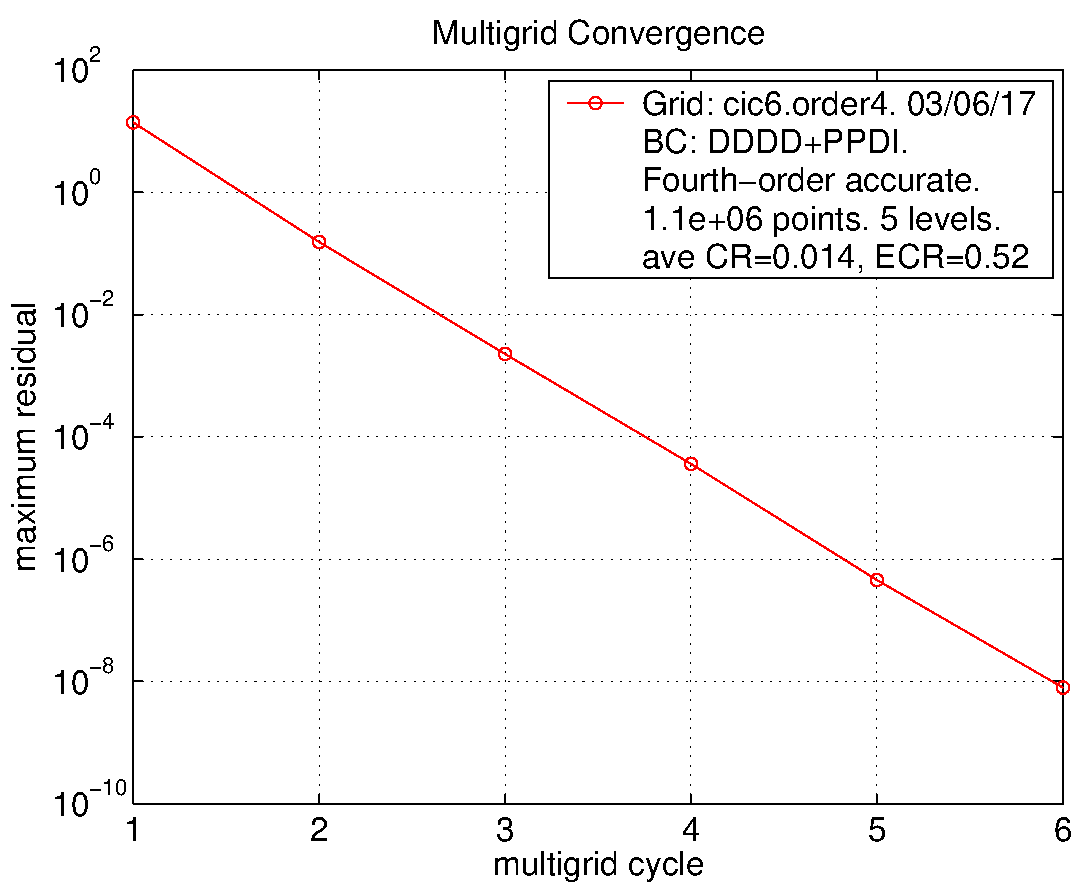
\includegraphics[width=.475\linewidth]{fig/residual_cic6_order4}
  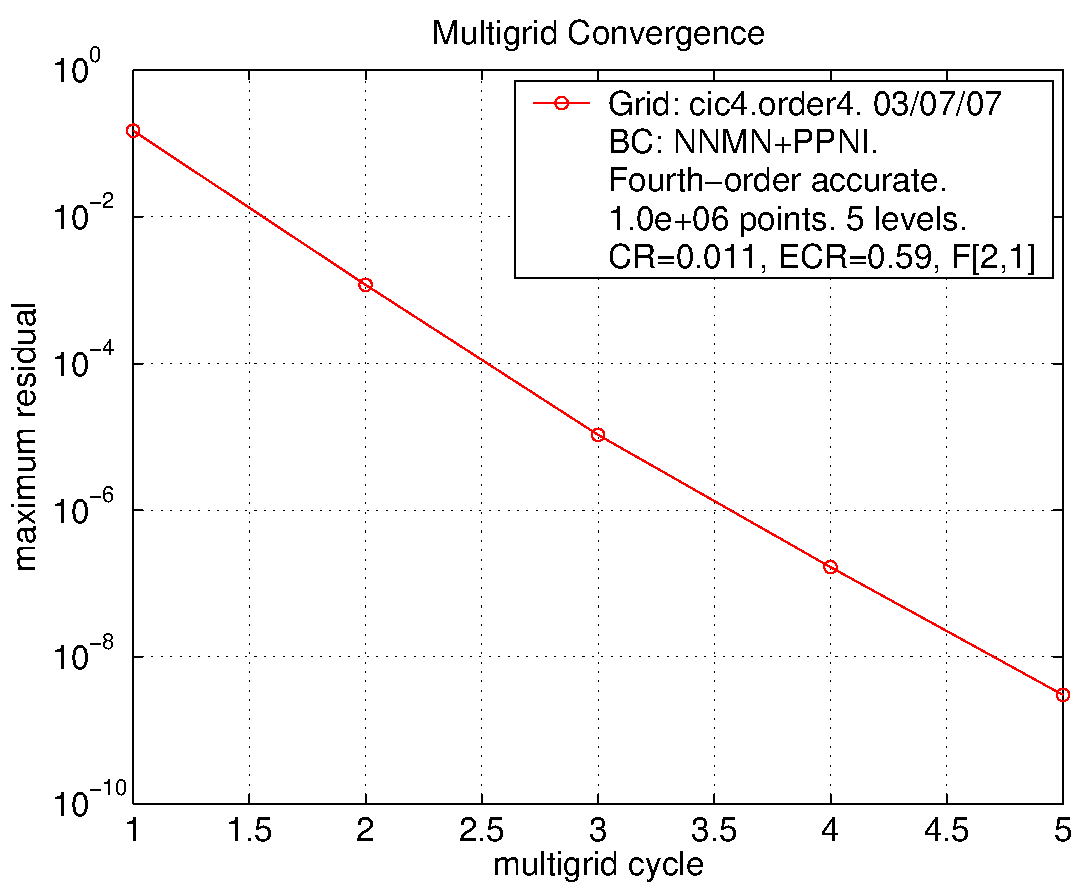
\includegraphics[width=.475\linewidth]{fig/residual_cic4_mixed_order4}
  \end{center} 
\caption{Convergence history for a circle-in-a-channel, fourth-order accurate, with IBS smoothing. Left: W[2,1], cic6.order4.
    Right: F[2,1], cic4.order4. }
\label{fig:square1024}
\end{figure}

% ===========================================================================
\begin{table}[hbt]
\begin{center}
{\tablefontsize
\begin{tabular}{|c|c|c|c|c|} \hline 
 $i$   & $\vert\vert\mbox{res}\vert\vert_\infty$  &  CR     &  WU    & ECR  \\   \hline 
 $ 1$  & $ 1.4e+01$ & $0.014$ & $ 6.1$ & $0.49$ \\ 
 $ 2$  & $ 1.5e-01$ & $0.011$ & $ 6.2$ & $0.48$ \\ 
 $ 3$  & $ 2.3e-03$ & $0.015$ & $ 6.2$ & $0.51$ \\ 
 $ 4$  & $ 3.6e-05$ & $0.016$ & $ 6.2$ & $0.51$ \\ 
 $ 5$  & $ 4.6e-07$ & $0.013$ & $ 6.2$ & $0.50$ \\ 
 $ 6$  & $ 7.9e-09$ & $0.017$ & $ 6.3$ & $0.53$ \\ 
\hline 
\multicolumn{5}{|c|}{Grid: cic6.order4. 03/06/18}  \\
\multicolumn{5}{|c|}{BC: DDDD+PPDI.}  \\
\multicolumn{5}{|c|}{Fourth-order accurate.}  \\
\multicolumn{5}{|c|}{Trigonometric solution.}  \\
\multicolumn{5}{|c|}{** F[2,1]: rb $\omega=1.15$}  \\
\multicolumn{5}{|c|}{1.13e+06 grid-points. 5 levels.}  \\
\multicolumn{5}{|c|}{Average CR=$0.014$, ECR=$0.50$.}  \\
\multicolumn{5}{|c|}{time/cycle = 2.12e+00 s.}  \\
\hline 
\end{tabular}
\begin{tabular}{|c|c|c|c|c|} \hline 
 $i$   & $\vert\vert\mbox{res}\vert\vert_\infty$  &  CR     &  WU    & ECR  \\   \hline 
 $ 1$  & $ 1.4e+01$ & $0.014$ & $ 6.3$ & $0.51$ \\ 
 $ 2$  & $ 1.5e-01$ & $0.011$ & $ 6.4$ & $0.50$ \\ 
 $ 3$  & $ 2.3e-03$ & $0.015$ & $ 6.5$ & $0.52$ \\ 
 $ 4$  & $ 3.6e-05$ & $0.016$ & $ 6.5$ & $0.53$ \\ 
 $ 5$  & $ 4.6e-07$ & $0.013$ & $ 6.5$ & $0.51$ \\ 
 $ 6$  & $ 7.9e-09$ & $0.017$ & $ 6.6$ & $0.54$ \\ 
 $ 7$  & $ 1.1e-10$ & $0.014$ & $ 6.8$ & $0.53$ \\ 
\hline 
\multicolumn{5}{|c|}{Grid: cic6.order4. 03/06/17}  \\
\multicolumn{5}{|c|}{BC: DDDD+PPDI.}  \\
\multicolumn{5}{|c|}{Fourth-order accurate.}  \\
\multicolumn{5}{|c|}{Trigonometric solution.}  \\
\multicolumn{5}{|c|}{W[2,1]: rb $\omega=1.15$ IBS:2-4-2}  \\
\multicolumn{5}{|c|}{1.13e+06 grid-points. 5 levels.}  \\
\multicolumn{5}{|c|}{Average CR=$0.014$, ECR=$0.52$.}  \\
\multicolumn{5}{|c|}{time/cycle = 2.37e+00 s.}  \\
\hline 
\end{tabular}
\begin{tabular}{|c|c|c|c|c|} \hline 
 $i$   & $\vert\vert\mbox{res}\vert\vert_\infty$  &  CR     &  WU    & ECR  \\   \hline 
 $ 1$  & $ 8.7e+00$ & $0.016$ & $ 6.2$ & $0.51$ \\ 
 $ 2$  & $ 1.2e-01$ & $0.013$ & $ 6.2$ & $0.50$ \\ 
 $ 3$  & $ 2.5e-03$ & $0.021$ & $ 6.2$ & $0.54$ \\ 
 $ 4$  & $ 4.0e-05$ & $0.016$ & $ 6.3$ & $0.52$ \\ 
 $ 5$  & $ 7.3e-07$ & $0.018$ & $ 6.3$ & $0.53$ \\ 
 $ 6$  & $ 1.1e-08$ & $0.016$ & $ 6.2$ & $0.51$ \\ 
 $ 7$  & $ 4.1e-10$ & $0.036$ & $ 6.3$ & $0.59$ \\ 
\hline 
\multicolumn{5}{|c|}{Grid: cic6.order4. 03/06/13}  \\
\multicolumn{5}{|c|}{BC: DDDD+PPDI.}  \\
\multicolumn{5}{|c|}{Fourth-order accurate.}  \\
\multicolumn{5}{|c|}{Trigonometric solution.}  \\
\multicolumn{5}{|c|}{W[2,1]: rb $\omega=1.15$}  \\
\multicolumn{5}{|c|}{1.13e+06 grid-points. 5 levels.}  \\
\multicolumn{5}{|c|}{Average CR=$0.019$, ECR=$0.53$.}  \\
\multicolumn{5}{|c|}{time/cycle = 2.12e+00 s.}  \\
\hline 
\end{tabular}
\begin{tabular}{|c|c|c|c|c|} \hline 
 $i$   & $\vert\vert\mbox{res}\vert\vert_\infty$  &  CR     &  WU    & ECR  \\   \hline 
 $ 1$  & $ 8.7e+00$ & $0.016$ & $ 6.2$ & $0.51$ \\ 
 $ 2$  & $ 1.2e-01$ & $0.013$ & $ 6.2$ & $0.50$ \\ 
 $ 3$  & $ 2.5e-03$ & $0.021$ & $ 6.2$ & $0.54$ \\ 
 $ 4$  & $ 4.0e-05$ & $0.016$ & $ 6.3$ & $0.52$ \\ 
 $ 5$  & $ 7.3e-07$ & $0.018$ & $ 6.3$ & $0.53$ \\ 
 $ 6$  & $ 1.1e-08$ & $0.016$ & $ 6.2$ & $0.51$ \\ 
 $ 7$  & $ 4.1e-10$ & $0.036$ & $ 6.3$ & $0.59$ \\ 
\hline 
\multicolumn{5}{|c|}{Grid: cic6.order4. 03/06/13}  \\
\multicolumn{5}{|c|}{BC: DDDD+PPDI.}  \\
\multicolumn{5}{|c|}{Fourth-order accurate.}  \\
\multicolumn{5}{|c|}{Trigonometric solution.}  \\
\multicolumn{5}{|c|}{W[2,1]: rb $\omega=1.15$ odd-sym-lower}  \\
\multicolumn{5}{|c|}{1.13e+06 grid-points. 5 levels.}  \\
\multicolumn{5}{|c|}{Average CR=$0.019$, ECR=$0.53$.}  \\
\multicolumn{5}{|c|}{time/cycle = 2.11e+00 s.}  \\
\hline 
\end{tabular}
\begin{tabular}{|c|c|c|c|c|} \hline 
 $i$   & $\vert\vert\mbox{res}\vert\vert_\infty$  &  CR     &  WU    & ECR  \\   \hline 
 $ 1$  & $ 7.6e+00$ & $0.012$ & $ 5.0$ & $0.41$ \\ 
 $ 2$  & $ 1.2e-01$ & $0.016$ & $ 5.2$ & $0.45$ \\ 
 $ 3$  & $ 2.4e-03$ & $0.019$ & $ 5.1$ & $0.46$ \\ 
 $ 4$  & $ 1.8e-04$ & $0.074$ & $ 5.2$ & $0.60$ \\ 
 $ 5$  & $ 1.4e-05$ & $0.079$ & $ 5.2$ & $0.61$ \\ 
 $ 6$  & $ 1.0e-06$ & $0.075$ & $ 5.4$ & $0.62$ \\ 
 $ 7$  & $ 7.3e-08$ & $0.070$ & $ 5.4$ & $0.61$ \\ 
 $ 8$  & $ 5.2e-09$ & $0.071$ & $ 5.4$ & $0.61$ \\ 
\hline 
\multicolumn{5}{|c|}{Grid: cic6.order4. 03/06/13}  \\
\multicolumn{5}{|c|}{BC: DDDD+PPDI.}  \\
\multicolumn{5}{|c|}{Fourth-order accurate.}  \\
\multicolumn{5}{|c|}{Trigonometric solution.}  \\
\multicolumn{5}{|c|}{V[2,1]: rb $\omega=1.15$}  \\
\multicolumn{5}{|c|}{1.13e+06 grid-points. 5 levels.}  \\
\multicolumn{5}{|c|}{Average CR=$0.041$, ECR=$0.54$.}  \\
\multicolumn{5}{|c|}{time/cycle = 1.48e+00 s.}  \\
\hline 
\end{tabular}
\begin{tabular}{|c|c|c|c|c|} \hline 
 $i$   & $\vert\vert\mbox{res}\vert\vert_\infty$  &  CR     &  WU    & ECR  \\   \hline 
 $ 1$  & $ 3.1e+00$ & $0.014$ & $ 6.3$ & $0.51$ \\ 
 $ 2$  & $ 3.5e-02$ & $0.011$ & $ 6.7$ & $0.52$ \\ 
 $ 3$  & $ 4.8e-04$ & $0.014$ & $ 7.1$ & $0.55$ \\ 
 $ 4$  & $ 8.0e-06$ & $0.017$ & $ 7.3$ & $0.57$ \\ 
 $ 5$  & $ 1.1e-07$ & $0.013$ & $ 6.9$ & $0.53$ \\ 
 $ 6$  & $ 1.8e-09$ & $0.017$ & $ 6.4$ & $0.52$ \\ 
\hline 
\multicolumn{5}{|c|}{Grid: cic3.order4. 03/06/17}  \\
\multicolumn{5}{|c|}{BC: DDDD+PPDI.}  \\
\multicolumn{5}{|c|}{Fourth-order accurate.}  \\
\multicolumn{5}{|c|}{Trigonometric solution.}  \\
\multicolumn{5}{|c|}{W[2,1]: rb $\omega=1.15$ IBS:2-4-2}  \\
\multicolumn{5}{|c|}{2.60e+05 grid-points. 4 levels.}  \\
\multicolumn{5}{|c|}{Average CR=$0.014$, ECR=$0.53$.}  \\
\multicolumn{5}{|c|}{time/cycle = 6.94e-01 s.}  \\
\hline 
\end{tabular}
% \qquad % --------------------------------------------------------------------
% \begin{tabular}{|c|c|c|c|c|} \hline 
%  $i$   & res      & rate    &  WU    & ECR  \\   \hline 
%  $ 1$  & $ 9.4e+01$ & $0.025$ & $ 6.8$ & $0.58$ \\ 
%  $ 2$  & $ 2.0e+00$ & $0.021$ & $ 6.9$ & $0.57$ \\ 
%  $ 3$  & $ 2.7e-02$ & $0.013$ & $ 7.2$ & $0.55$ \\ 
%  $ 4$  & $ 1.6e-03$ & $0.061$ & $ 7.1$ & $0.67$ \\ 
%  $ 5$  & $ 2.2e-04$ & $0.133$ & $ 7.0$ & $0.75$ \\ 
%  $ 6$  & $ 2.6e-05$ & $0.118$ & $ 6.8$ & $0.73$ \\ 
%  $ 7$  & $ 3.1e-06$ & $0.122$ & $ 6.7$ & $0.73$ \\ 
%  $ 8$  & $ 3.9e-07$ & $0.124$ & $ 6.7$ & $0.73$ \\ 
%  $ 9$  & $ 4.8e-08$ & $0.123$ & $ 6.7$ & $0.73$ \\ 
%  $10$  & $ 5.9e-09$ & $0.123$ & $ 6.7$ & $0.73$ \\ 
%  $11$  & $ 7.5e-10$ & $0.129$ & $ 6.7$ & $0.73$ \\ 
% \hline 
% \multicolumn{5}{|c|}{Grid: cic6.order4.}  \\
% \multicolumn{5}{|c|}{Dirichlet boundary conditions.}  \\
% \multicolumn{5}{|c|}{Trigonometric solution.}  \\
% \multicolumn{5}{|c|}{Fourth-order accurate.}  \\
% \multicolumn{5}{|c|}{Smoother lz2[2,1]}  \\
% \multicolumn{5}{|c|}{1.13e+06 grid-points. 5 levels.}  \\
% \multicolumn{5}{|c|}{Average CR=$0.070$, ECR=$0.68$.}  \\
% \hline 
% \end{tabular}
%\qquad % --------------------------------------------------------------------
% \vskip\baselineskip
% \qquad % --------------------------------------------------------------------
% \begin{tabular}{|c|c|c|c|c|} \hline 
%  $i$   & $\vert\vert\mbox{res}\vert\vert_\infty$  &  CR     &  WU    & ECR  \\   \hline 
%  $ 1$  & $ 8.7e+00$ & $0.016$ & $ 6.2$ & $0.51$ \\ 
%  $ 2$  & $ 1.2e-01$ & $0.014$ & $ 6.2$ & $0.50$ \\ 
%  $ 3$  & $ 2.5e-03$ & $0.021$ & $ 6.2$ & $0.54$ \\ 
%  $ 4$  & $ 4.0e-05$ & $0.016$ & $ 6.3$ & $0.52$ \\ 
%  $ 5$  & $ 8.0e-07$ & $0.020$ & $ 6.3$ & $0.54$ \\ 
%  $ 6$  & $ 5.8e-08$ & $0.072$ & $ 6.3$ & $0.66$ \\ 
%  $ 7$  & $ 2.8e-09$ & $0.048$ & $ 6.3$ & $0.62$ \\ 
% \hline 
% \multicolumn{5}{|c|}{Grid: cic6.order4. 2003/06/06.}  \\
% \multicolumn{5}{|c|}{BC: DDDD+PPDI.}  \\
% \multicolumn{5}{|c|}{Fourth-order accurate.}  \\
% \multicolumn{5}{|c|}{Trigonometric solution.}  \\
% \multicolumn{5}{|c|}{W[2,1]: rb $\omega=1.15$}  \\
% \multicolumn{5}{|c|}{1.13e+06 grid-points. 5 levels.}  \\
% \multicolumn{5}{|c|}{Average CR=$0.024$, ECR=$0.55$.}  \\
% \multicolumn{5}{|c|}{time/cycle = 1.99e+00 s.}  \\
% \hline 
% \end{tabular}
} %\tablefontsize
\end{center}
\caption{Multigrid convergence rates for a circle-in-a-channel, fourth-order accuracy.
     IBS:g-l-s interpolation smoothing, g-iterations, l-layers, s-sub-smooths  }
 \label{tab:square4} 
\end{table}





\begin{table}[hbt]
\begin{center}
{\tablefontsize
\begin{tabular}{|c|c|c|c|c|} \hline 
 $i$   & $\vert\vert\mbox{res}\vert\vert_\infty$  &  CR     &  WU    & ECR  \\   \hline 
 $ 1$  & $ 8.7e+00$ & $0.016$ & $ 6.2$ & $0.51$ \\ 
 $ 2$  & $ 1.2e-01$ & $0.013$ & $ 6.2$ & $0.50$ \\ 
 $ 3$  & $ 2.5e-03$ & $0.021$ & $ 6.2$ & $0.54$ \\ 
 $ 4$  & $ 4.0e-05$ & $0.016$ & $ 6.3$ & $0.52$ \\ 
 $ 5$  & $ 7.3e-07$ & $0.018$ & $ 6.3$ & $0.53$ \\ 
 $ 6$  & $ 1.1e-08$ & $0.016$ & $ 6.2$ & $0.51$ \\ 
 $ 7$  & $ 4.1e-10$ & $0.036$ & $ 6.3$ & $0.59$ \\ 
\hline 
\multicolumn{5}{|c|}{Grid: cic6.order4. 03/06/09}  \\
\multicolumn{5}{|c|}{BC: DDDD+PPDI.}  \\
\multicolumn{5}{|c|}{Fourth-order accurate.}  \\
\multicolumn{5}{|c|}{Trigonometric solution.}  \\
\multicolumn{5}{|c|}{W[2,1]: rb $\omega=1.15$ ALT}  \\
\multicolumn{5}{|c|}{1.13e+06 grid-points. 5 levels.}  \\
\multicolumn{5}{|c|}{Average CR=$0.019$, ECR=$0.53$.}  \\
\multicolumn{5}{|c|}{time/cycle = 2.10e+00 s.}  \\
\hline 
\end{tabular}
%\qquad % --------------------------------------------------------------------
\begin{tabular}{|c|c|c|c|c|} \hline 
 $i$   & $\vert\vert\mbox{res}\vert\vert_\infty$  &  CR     &  WU    & ECR  \\   \hline 
 $ 1$  & $ 4.0e+01$ & $0.018$ & $ 6.2$ & $0.52$ \\ 
 $ 2$  & $ 6.4e-01$ & $0.016$ & $ 6.2$ & $0.52$ \\ 
 $ 3$  & $ 9.9e-03$ & $0.016$ & $ 6.2$ & $0.51$ \\ 
 $ 4$  & $ 1.2e-04$ & $0.012$ & $ 6.3$ & $0.50$ \\ 
 $ 5$  & $ 2.1e-06$ & $0.017$ & $ 6.2$ & $0.52$ \\ 
 $ 6$  & $ 3.9e-08$ & $0.018$ & $ 6.3$ & $0.53$ \\ 
 $ 7$  & $ 6.5e-10$ & $0.017$ & $ 6.4$ & $0.53$ \\ 
\hline 
\multicolumn{5}{|c|}{Grid: cic7.order4. 03/06/09}  \\
\multicolumn{5}{|c|}{BC: DDDD+PPDI.}  \\
\multicolumn{5}{|c|}{Fourth-order accurate.}  \\
\multicolumn{5}{|c|}{Trigonometric solution.}  \\
\multicolumn{5}{|c|}{W[2,1]: rb $\omega=1.16$ ALT}  \\
\multicolumn{5}{|c|}{4.36e+06 grid-points. 5 levels.}  \\
\multicolumn{5}{|c|}{Average CR=$0.016$, ECR=$0.52$.}  \\
\multicolumn{5}{|c|}{time/cycle = 6.98e+00 s.}  \\
\hline 
\end{tabular}
%\qquad % --------------------------------------------------------------------
%\vskip\baselineskip
\begin{tabular}{|c|c|c|c|c|} \hline 
 $i$   & $\vert\vert\mbox{res}\vert\vert_\infty$  &  CR     &  WU    & ECR  \\   \hline 
 $ 1$  & $ 4.5e+01$ & $0.020$ & $ 6.2$ & $0.53$ \\ 
 $ 2$  & $ 7.6e-01$ & $0.017$ & $ 6.2$ & $0.52$ \\ 
 $ 3$  & $ 1.2e-02$ & $0.016$ & $ 6.2$ & $0.52$ \\ 
 $ 4$  & $ 1.7e-04$ & $0.014$ & $ 6.2$ & $0.51$ \\ 
 $ 5$  & $ 4.7e-06$ & $0.027$ & $ 6.3$ & $0.56$ \\ 
 $ 6$  & $ 4.5e-07$ & $0.096$ & $ 6.4$ & $0.69$ \\ 
 $ 7$  & $ 4.7e-08$ & $0.105$ & $ 6.4$ & $0.70$ \\ 
 $ 8$  & $ 4.8e-09$ & $0.103$ & $ 6.4$ & $0.70$ \\ 
\hline 
\multicolumn{5}{|c|}{Grid: cic7.order4. 03/06/09}  \\
\multicolumn{5}{|c|}{BC: DDDD+PPDI.}  \\
\multicolumn{5}{|c|}{Fourth-order accurate.}  \\
\multicolumn{5}{|c|}{Trigonometric solution.}  \\
\multicolumn{5}{|c|}{W[2,1]: rb $\omega=1.16$ 1..ng }  \\
\multicolumn{5}{|c|}{4.36e+06 grid-points. 5 levels.}  \\
\multicolumn{5}{|c|}{Average CR=$0.035$, ECR=$0.59$.}  \\
\multicolumn{5}{|c|}{time/cycle = 7.03e+00 s.}  \\
\hline 
\end{tabular}
%\qquad % --------------------------------------------------------------------
\begin{tabular}{|c|c|c|c|c|} \hline 
 $i$   & $\vert\vert\mbox{res}\vert\vert_\infty$  &  CR     &  WU    & ECR  \\   \hline 
 $ 1$  & $ 3.8e+01$ & $0.017$ & $ 6.2$ & $0.52$ \\ 
 $ 2$  & $ 6.2e-01$ & $0.016$ & $ 6.2$ & $0.52$ \\ 
 $ 3$  & $ 8.7e-03$ & $0.014$ & $ 6.2$ & $0.51$ \\ 
 $ 4$  & $ 1.2e-04$ & $0.013$ & $ 6.2$ & $0.50$ \\ 
 $ 5$  & $ 2.1e-06$ & $0.018$ & $ 6.3$ & $0.53$ \\ 
 $ 6$  & $ 4.1e-08$ & $0.020$ & $ 6.3$ & $0.54$ \\ 
\hline 
\multicolumn{5}{|c|}{Grid: cic7.order4. 03/06/09}  \\
\multicolumn{5}{|c|}{BC: DDDD+PPDI.}  \\
\multicolumn{5}{|c|}{Fourth-order accurate.}  \\
\multicolumn{5}{|c|}{Trigonometric solution.}  \\
\multicolumn{5}{|c|}{W[2,1]: rb $\omega=1.16$ ng..1}  \\
\multicolumn{5}{|c|}{4.36e+06 grid-points. 5 levels.}  \\
\multicolumn{5}{|c|}{Average CR=$0.016$, ECR=$0.52$.}  \\
\multicolumn{5}{|c|}{time/cycle = 7.11e+00 s.}  \\
\hline 
\end{tabular}
\begin{tabular}{|c|c|c|c|c|} \hline 
 $i$   & $\vert\vert\mbox{res}\vert\vert_\infty$  &  CR     &  WU    & ECR  \\   \hline 
 $ 1$  & $ 2.6e+01$ & $0.024$ & $ 6.5$ & $0.56$ \\ 
 $ 2$  & $ 5.5e-01$ & $0.021$ & $ 6.5$ & $0.55$ \\ 
 $ 3$  & $ 1.1e-02$ & $0.020$ & $ 6.5$ & $0.55$ \\ 
 $ 4$  & $ 2.7e-04$ & $0.024$ & $ 6.5$ & $0.56$ \\ 
 $ 5$  & $ 6.8e-06$ & $0.025$ & $ 6.5$ & $0.57$ \\ 
 $ 6$  & $ 1.7e-07$ & $0.025$ & $ 6.5$ & $0.57$ \\ 
 $ 7$  & $ 4.9e-09$ & $0.028$ & $ 6.5$ & $0.58$ \\ 
\hline 
\multicolumn{5}{|c|}{Grid: cic6.order4. 03/06/10}  \\
\multicolumn{5}{|c|}{BC: DDDD+PPDI.}  \\
\multicolumn{5}{|c|}{Fourth-order accurate.}  \\
\multicolumn{5}{|c|}{Trigonometric solution.}  \\
\multicolumn{5}{|c|}{W[2,1]: rb $\omega=1.15$, alz $\omega=1.00$}  \\
\multicolumn{5}{|c|}{1.13e+06 grid-points. 5 levels.}  \\
\multicolumn{5}{|c|}{Average CR=$0.024$, ECR=$0.56$.}  \\
\multicolumn{5}{|c|}{time/cycle = 2.09e+00 s.}  \\
\hline 
\end{tabular}
} %\tablefontsize
\end{center}
\caption{Multigrid convergence rates for a circle-in-a-channel, fourth-order accuracy.
  ALT=order of grids in smooth is altered every cycle.}
 \label{tab:cic4} 
\end{table}


\begin{table}[hbt]
\begin{center}
{\tablefontsize
\begin{tabular}{|c|c|c|c|c|} \hline 
 $i$   & $\vert\vert\mbox{res}\vert\vert_\infty$  &  CR     &  WU    & ECR  \\   \hline 
 $ 1$  & $ 8.7e+00$ & $0.016$ & $ 6.2$ & $0.51$ \\ 
 $ 2$  & $ 1.2e-01$ & $0.013$ & $ 6.2$ & $0.50$ \\ 
 $ 3$  & $ 2.5e-03$ & $0.021$ & $ 6.2$ & $0.54$ \\ 
 $ 4$  & $ 4.0e-05$ & $0.016$ & $ 6.3$ & $0.52$ \\ 
 $ 5$  & $ 7.3e-07$ & $0.018$ & $ 6.3$ & $0.53$ \\ 
 $ 6$  & $ 1.1e-08$ & $0.016$ & $ 6.2$ & $0.51$ \\ 
 $ 7$  & $ 4.1e-10$ & $0.036$ & $ 6.3$ & $0.59$ \\ 
\hline 
\multicolumn{5}{|c|}{Grid: cic6.order4. 03/06/09}  \\
\multicolumn{5}{|c|}{BC: DDDD+PPDI.}  \\
\multicolumn{5}{|c|}{Fourth-order accurate.}  \\
\multicolumn{5}{|c|}{Trigonometric solution.}  \\
\multicolumn{5}{|c|}{W[2,1]: rb $\omega=1.15$ ALT}  \\
\multicolumn{5}{|c|}{1.13e+06 grid-points. 5 levels.}  \\
\multicolumn{5}{|c|}{Average CR=$0.019$, ECR=$0.53$.}  \\
\multicolumn{5}{|c|}{time/cycle = 2.10e+00 s.}  \\
\hline 
\end{tabular}
%\qquad % --------------------------------------------------------------------
\begin{tabular}{|c|c|c|c|c|} \hline 
 $i$   & $\vert\vert\mbox{res}\vert\vert_\infty$  &  CR     &  WU    & ECR  \\   \hline 
 $ 1$  & $ 4.0e+01$ & $0.018$ & $ 6.2$ & $0.52$ \\ 
 $ 2$  & $ 6.4e-01$ & $0.016$ & $ 6.2$ & $0.52$ \\ 
 $ 3$  & $ 9.9e-03$ & $0.016$ & $ 6.2$ & $0.51$ \\ 
 $ 4$  & $ 1.2e-04$ & $0.012$ & $ 6.3$ & $0.50$ \\ 
 $ 5$  & $ 2.1e-06$ & $0.017$ & $ 6.2$ & $0.52$ \\ 
 $ 6$  & $ 3.9e-08$ & $0.018$ & $ 6.3$ & $0.53$ \\ 
 $ 7$  & $ 6.5e-10$ & $0.017$ & $ 6.4$ & $0.53$ \\ 
\hline 
\multicolumn{5}{|c|}{Grid: cic7.order4. 03/06/09}  \\
\multicolumn{5}{|c|}{BC: DDDD+PPDI.}  \\
\multicolumn{5}{|c|}{Fourth-order accurate.}  \\
\multicolumn{5}{|c|}{Trigonometric solution.}  \\
\multicolumn{5}{|c|}{W[2,1]: rb $\omega=1.16$ ALT}  \\
\multicolumn{5}{|c|}{4.36e+06 grid-points. 5 levels.}  \\
\multicolumn{5}{|c|}{Average CR=$0.016$, ECR=$0.52$.}  \\
\multicolumn{5}{|c|}{time/cycle = 6.98e+00 s.}  \\
\hline 
\end{tabular}
%\qquad % --------------------------------------------------------------------
%\vskip\baselineskip
\begin{tabular}{|c|c|c|c|c|} \hline 
 $i$   & $\vert\vert\mbox{res}\vert\vert_\infty$  &  CR     &  WU    & ECR  \\   \hline 
 $ 1$  & $ 4.5e+01$ & $0.020$ & $ 6.2$ & $0.53$ \\ 
 $ 2$  & $ 7.6e-01$ & $0.017$ & $ 6.2$ & $0.52$ \\ 
 $ 3$  & $ 1.2e-02$ & $0.016$ & $ 6.2$ & $0.52$ \\ 
 $ 4$  & $ 1.7e-04$ & $0.014$ & $ 6.2$ & $0.51$ \\ 
 $ 5$  & $ 4.7e-06$ & $0.027$ & $ 6.3$ & $0.56$ \\ 
 $ 6$  & $ 4.5e-07$ & $0.096$ & $ 6.4$ & $0.69$ \\ 
 $ 7$  & $ 4.7e-08$ & $0.105$ & $ 6.4$ & $0.70$ \\ 
 $ 8$  & $ 4.8e-09$ & $0.103$ & $ 6.4$ & $0.70$ \\ 
\hline 
\multicolumn{5}{|c|}{Grid: cic7.order4. 03/06/09}  \\
\multicolumn{5}{|c|}{BC: DDDD+PPDI.}  \\
\multicolumn{5}{|c|}{Fourth-order accurate.}  \\
\multicolumn{5}{|c|}{Trigonometric solution.}  \\
\multicolumn{5}{|c|}{W[2,1]: rb $\omega=1.16$ 1..ng }  \\
\multicolumn{5}{|c|}{4.36e+06 grid-points. 5 levels.}  \\
\multicolumn{5}{|c|}{Average CR=$0.035$, ECR=$0.59$.}  \\
\multicolumn{5}{|c|}{time/cycle = 7.03e+00 s.}  \\
\hline 
\end{tabular}
%\qquad % --------------------------------------------------------------------
\begin{tabular}{|c|c|c|c|c|} \hline 
 $i$   & $\vert\vert\mbox{res}\vert\vert_\infty$  &  CR     &  WU    & ECR  \\   \hline 
 $ 1$  & $ 3.8e+01$ & $0.017$ & $ 6.2$ & $0.52$ \\ 
 $ 2$  & $ 6.2e-01$ & $0.016$ & $ 6.2$ & $0.52$ \\ 
 $ 3$  & $ 8.7e-03$ & $0.014$ & $ 6.2$ & $0.51$ \\ 
 $ 4$  & $ 1.2e-04$ & $0.013$ & $ 6.2$ & $0.50$ \\ 
 $ 5$  & $ 2.1e-06$ & $0.018$ & $ 6.3$ & $0.53$ \\ 
 $ 6$  & $ 4.1e-08$ & $0.020$ & $ 6.3$ & $0.54$ \\ 
\hline 
\multicolumn{5}{|c|}{Grid: cic7.order4. 03/06/09}  \\
\multicolumn{5}{|c|}{BC: DDDD+PPDI.}  \\
\multicolumn{5}{|c|}{Fourth-order accurate.}  \\
\multicolumn{5}{|c|}{Trigonometric solution.}  \\
\multicolumn{5}{|c|}{W[2,1]: rb $\omega=1.16$ ng..1}  \\
\multicolumn{5}{|c|}{4.36e+06 grid-points. 5 levels.}  \\
\multicolumn{5}{|c|}{Average CR=$0.016$, ECR=$0.52$.}  \\
\multicolumn{5}{|c|}{time/cycle = 7.11e+00 s.}  \\
\hline 
\end{tabular}
} %\tablefontsize
\end{center}
\caption{Multigrid convergence rates for a circle-in-a-channel, fourth-order accuracy.
  ALT=order of grids in smooth is altered every cycle.}
 \label{tab:cic4} 
\end{table}


% ===========================================================================

% *************************************************************************************
\clearpage
\subsubsection{Fourth-order accurate with Neumann or mixed boundary conditions.}
\begin{table}[hbt]
\begin{center}
{\tablefontsize
\begin{tabular}{|c|c|c|c|c|} \hline 
 $i$   & $\vert\vert\mbox{res}\vert\vert_\infty$  &  CR     &  WU    & ECR  \\   \hline 
 $ 1$  & $ 2.3e-01$ & $0.010$ & $ 6.6$ & $0.50$ \\ 
 $ 2$  & $ 1.8e-03$ & $0.008$ & $ 6.9$ & $0.50$ \\ 
 $ 3$  & $ 1.6e-05$ & $0.009$ & $ 6.9$ & $0.51$ \\ 
 $ 4$  & $ 2.2e-07$ & $0.014$ & $ 6.9$ & $0.54$ \\ 
 $ 5$  & $ 4.0e-09$ & $0.018$ & $ 6.9$ & $0.56$ \\ 
\hline 
\multicolumn{5}{|c|}{Grid: cic7.order4. 03/07/04}  \\
\multicolumn{5}{|c|}{BC: NNMN+PPNI.}  \\
\multicolumn{5}{|c|}{Fourth-order accurate.}  \\
\multicolumn{5}{|c|}{Trigonometric solution.}  \\
\multicolumn{5}{|c|}{F[2,1]: rb $\omega=1.16$}  \\
\multicolumn{5}{|c|}{4.36e+06 grid-points. 5 levels.}  \\
\multicolumn{5}{|c|}{Average CR=$0.011$, ECR=$0.52$.}  \\
\multicolumn{5}{|c|}{time/cycle = 9.03e+00 s.}  \\
\hline 
\end{tabular}
\begin{tabular}{|c|c|c|c|c|} \hline 
 $i$   & $\vert\vert\mbox{res}\vert\vert_\infty$  &  CR     &  WU    & ECR  \\   \hline 
 $ 1$  & $ 1.5e-01$ & $0.010$ & $ 7.8$ & $0.55$ \\ 
 $ 2$  & $ 1.2e-03$ & $0.008$ & $ 8.6$ & $0.57$ \\ 
 $ 3$  & $ 1.1e-05$ & $0.009$ & $ 8.6$ & $0.58$ \\ 
 $ 4$  & $ 1.7e-07$ & $0.016$ & $ 8.6$ & $0.62$ \\ 
 $ 5$  & $ 3.0e-09$ & $0.018$ & $ 8.6$ & $0.63$ \\ 
\hline 
\multicolumn{5}{|c|}{Grid: cic4.order4. 03/07/04}  \\
\multicolumn{5}{|c|}{BC: NNMN+PPNI. NO-AVE}  \\
\multicolumn{5}{|c|}{Fourth-order accurate.}  \\
\multicolumn{5}{|c|}{Trigonometric solution.}  \\
\multicolumn{5}{|c|}{F[2,1]: rb $\omega=1.15$}  \\
\multicolumn{5}{|c|}{1.02e+06 grid-points. 5 levels.}  \\
\multicolumn{5}{|c|}{Average CR=$0.011$, ECR=$0.59$.}  \\
\multicolumn{5}{|c|}{time/cycle = 3.32e+00 s.}  \\
\hline 
\end{tabular}
\begin{tabular}{|c|c|c|c|c|} \hline 
 $i$   & $\vert\vert\mbox{res}\vert\vert_\infty$  &  CR     &  WU    & ECR  \\   \hline 
 $ 1$  & $ 3.8e-02$ & $0.010$ & $ 6.8$ & $0.51$ \\ 
 $ 2$  & $ 4.7e-04$ & $0.012$ & $ 6.9$ & $0.53$ \\ 
 $ 3$  & $ 1.1e-05$ & $0.022$ & $ 7.1$ & $0.59$ \\ 
 $ 4$  & $ 2.4e-07$ & $0.023$ & $ 7.1$ & $0.59$ \\ 
 $ 5$  & $ 5.5e-09$ & $0.023$ & $ 6.7$ & $0.57$ \\ 
\hline 
\multicolumn{5}{|c|}{Grid: cic4.order4. 03/07/04}  \\
\multicolumn{5}{|c|}{BC: NNMN+PPNI.}  \\
\multicolumn{5}{|c|}{Fourth-order accurate. NO-AVE}  \\
\multicolumn{5}{|c|}{Trigonometric solution.}  \\
\multicolumn{5}{|c|}{W[2,1]: rb $\omega=1.15$, lz1 $\omega=1.00$}  \\
\multicolumn{5}{|c|}{1.02e+06 grid-points. 5 levels.}  \\
\multicolumn{5}{|c|}{Average CR=$0.017$, ECR=$0.56$.}  \\
\multicolumn{5}{|c|}{time/cycle = 2.22e+00 s.}  \\
\hline 
\end{tabular}
\begin{tabular}{|c|c|c|c|c|} \hline 
 $i$   & $\vert\vert\mbox{res}\vert\vert_\infty$  &  CR     &  WU    & ECR  \\   \hline 
 $ 1$  & $ 1.5e-01$ & $0.010$ & $ 8.1$ & $0.56$ \\ 
 $ 2$  & $ 1.2e-03$ & $0.008$ & $ 8.8$ & $0.58$ \\ 
 $ 3$  & $ 1.1e-05$ & $0.009$ & $ 8.9$ & $0.59$ \\ 
 $ 4$  & $ 1.6e-07$ & $0.015$ & $ 8.9$ & $0.63$ \\ 
 $ 5$  & $ 3.0e-09$ & $0.018$ & $ 8.9$ & $0.64$ \\ 
\hline 
\multicolumn{5}{|c|}{Grid: cic4.order4. 03/07/04}  \\
\multicolumn{5}{|c|}{BC: NNMN+PPNI. NO-AVE}  \\
\multicolumn{5}{|c|}{Fourth-order accurate.}  \\
\multicolumn{5}{|c|}{Trigonometric solution.}  \\
\multicolumn{5}{|c|}{W[2,1]: rb $\omega=1.15$}  \\
\multicolumn{5}{|c|}{1.02e+06 grid-points. 5 levels.}  \\
\multicolumn{5}{|c|}{Average CR=$0.011$, ECR=$0.60$.}  \\
\multicolumn{5}{|c|}{time/cycle = 3.90e+00 s.}  \\
\hline 
\end{tabular}
\begin{tabular}{|c|c|c|c|c|} \hline 
 $i$   & $\vert\vert\mbox{res}\vert\vert_\infty$  &  CR     &  WU    & ECR  \\   \hline 
 $ 1$  & $ 7.7e+00$ & $0.016$ & $ 6.2$ & $0.51$ \\ 
 $ 2$  & $ 1.1e-01$ & $0.014$ & $ 6.5$ & $0.52$ \\ 
 $ 3$  & $ 2.2e-03$ & $0.020$ & $ 7.2$ & $0.58$ \\ 
 $ 4$  & $ 3.3e-05$ & $0.015$ & $ 7.8$ & $0.58$ \\ 
 $ 5$  & $ 6.3e-07$ & $0.019$ & $ 8.0$ & $0.61$ \\ 
 $ 6$  & $ 9.4e-09$ & $0.015$ & $ 7.7$ & $0.58$ \\ 
\hline 
\multicolumn{5}{|c|}{Grid: cic4.order4. 03/07/04}  \\
\multicolumn{5}{|c|}{BC: DDDD+PPNI. NO-AVE-CURV}  \\
\multicolumn{5}{|c|}{Fourth-order accurate.}  \\
\multicolumn{5}{|c|}{Trigonometric solution.}  \\
\multicolumn{5}{|c|}{W[2,1]: rb $\omega=1.15$}  \\
\multicolumn{5}{|c|}{1.02e+06 grid-points. 5 levels.}  \\
\multicolumn{5}{|c|}{Average CR=$0.016$, ECR=$0.57$.}  \\
\multicolumn{5}{|c|}{time/cycle = 2.76e+00 s.}  \\
\hline 
\end{tabular}
\begin{tabular}{|c|c|c|c|c|} \hline 
 $i$   & $\vert\vert\mbox{res}\vert\vert_\infty$  &  CR     &  WU    & ECR  \\   \hline 
 $ 1$  & $ 5.1e-02$ & $0.013$ & $ 7.0$ & $0.54$ \\ 
 $ 2$  & $ 4.6e-04$ & $0.009$ & $ 7.3$ & $0.53$ \\ 
 $ 3$  & $ 8.1e-06$ & $0.018$ & $ 7.7$ & $0.59$ \\ 
 $ 4$  & $ 1.7e-07$ & $0.021$ & $ 7.5$ & $0.60$ \\ 
 $ 5$  & $ 3.5e-09$ & $0.021$ & $ 6.9$ & $0.57$ \\ 
 $ 6$  & $ 9.7e-11$ & $0.028$ & $ 6.8$ & $0.59$ \\ 
\hline 
\multicolumn{5}{|c|}{Grid: cic4.order4. 03/07/04}  \\
\multicolumn{5}{|c|}{BC: NNMN+PPNI. NO-AVE-CURV}  \\
\multicolumn{5}{|c|}{Fourth-order accurate. NO-SPLIT-ALZ}  \\
\multicolumn{5}{|c|}{Trigonometric solution.}  \\
\multicolumn{5}{|c|}{W[2,1]: rb $\omega=1.15$, alz $\omega=1.00$}  \\
\multicolumn{5}{|c|}{1.02e+06 grid-points. 5 levels.}  \\
\multicolumn{5}{|c|}{Average CR=$0.017$, ECR=$0.57$.}  \\
\multicolumn{5}{|c|}{time/cycle = 2.82e+00 s.}  \\
\hline 
\end{tabular}
% \begin{tabular}{|c|c|c|c|c|} \hline 
%  $i$   & $\vert\vert\mbox{res}\vert\vert_\infty$  &  CR     &  WU    & ECR  \\   \hline 
%  $ 1$  & $ 5.3e+01$ & $0.040$ & $ 6.2$ & $0.59$ \\ 
%  $ 2$  & $ 2.4e+00$ & $0.046$ & $ 6.2$ & $0.61$ \\ 
%  $ 3$  & $ 1.2e-01$ & $0.047$ & $ 6.2$ & $0.61$ \\ 
%  $ 4$  & $ 5.5e-03$ & $0.048$ & $ 6.6$ & $0.63$ \\ 
%  $ 5$  & $ 4.0e-04$ & $0.073$ & $ 7.0$ & $0.69$ \\ 
%  $ 6$  & $ 6.5e-05$ & $0.162$ & $ 7.6$ & $0.79$ \\ 
%  $ 7$  & $ 6.7e-06$ & $0.102$ & $ 8.4$ & $0.76$ \\ 
%  $ 8$  & $ 6.5e-07$ & $0.097$ & $ 8.9$ & $0.77$ \\ 
%  $ 9$  & $ 8.0e-08$ & $0.123$ & $ 8.9$ & $0.79$ \\ 
% \hline 
% \multicolumn{5}{|c|}{Grid: cic4.order4. 03/06/08}  \\
% \multicolumn{5}{|c|}{BC: DDDD+PPNI.}  \\
% \multicolumn{5}{|c|}{Fourth-order accurate.}  \\
% \multicolumn{5}{|c|}{Trigonometric solution.}  \\
% \multicolumn{5}{|c|}{W[2,1]: rb $\omega=1.00$}  \\
% \multicolumn{5}{|c|}{1.02e+06 grid-points. 5 levels.}  \\
% \multicolumn{5}{|c|}{Average CR=$0.073$, ECR=$0.70$.}  \\
% \multicolumn{5}{|c|}{time/cycle = 2.65e+00 s.}  \\
% \hline 
% \end{tabular}
%\qquad % --------------------------------------------------------------------
% \begin{tabular}{|c|c|c|c|c|} \hline 
%  $i$   & $\vert\vert\mbox{res}\vert\vert_\infty$  &  CR     &  WU    & ECR  \\   \hline 
%  $ 1$  & $ 6.0e+01$ & $0.040$ & $ 6.2$ & $0.59$ \\ 
%  $ 2$  & $ 2.8e+00$ & $0.046$ & $ 6.2$ & $0.61$ \\ 
%  $ 3$  & $ 1.3e-01$ & $0.047$ & $ 6.2$ & $0.61$ \\ 
%  $ 4$  & $ 6.3e-03$ & $0.048$ & $ 6.3$ & $0.61$ \\ 
%  $ 5$  & $ 3.0e-04$ & $0.048$ & $ 6.6$ & $0.63$ \\ 
%  $ 6$  & $ 1.8e-05$ & $0.060$ & $ 7.2$ & $0.68$ \\ 
%  $ 7$  & $ 4.3e-06$ & $0.236$ & $ 7.8$ & $0.83$ \\ 
%  $ 8$  & $ 9.1e-07$ & $0.214$ & $ 8.2$ & $0.83$ \\ 
%  $ 9$  & $ 1.8e-07$ & $0.193$ & $ 8.2$ & $0.82$ \\ 
% \hline 
% \multicolumn{5}{|c|}{Grid: cic6.order4. 03/06/08}  \\
% \multicolumn{5}{|c|}{BC: DDDD+PPNI.}  \\
% \multicolumn{5}{|c|}{Fourth-order accurate.}  \\
% \multicolumn{5}{|c|}{Trigonometric solution.}  \\
% \multicolumn{5}{|c|}{W[2,1]: rb $\omega=1.00$}  \\
% \multicolumn{5}{|c|}{1.13e+06 grid-points. 5 levels.}  \\
% \multicolumn{5}{|c|}{Average CR=$0.079$, ECR=$0.69$.}  \\
% \multicolumn{5}{|c|}{time/cycle = 2.62e+00 s.}  \\
% \hline 
% \end{tabular}
% %\qquad % --------------------------------------------------------------------
% %\vskip\baselineskip
% \begin{tabular}{|c|c|c|c|c|} \hline 
%  $i$   & $\vert\vert\mbox{res}\vert\vert_\infty$  &  CR     &  WU    & ECR  \\   \hline 
%  $ 1$  & $ 4.0e+01$ & $0.018$ & $ 6.2$ & $0.52$ \\ 
%  $ 2$  & $ 6.4e-01$ & $0.016$ & $ 6.2$ & $0.51$ \\ 
%  $ 3$  & $ 9.9e-03$ & $0.016$ & $ 6.2$ & $0.51$ \\ 
%  $ 4$  & $ 1.2e-04$ & $0.012$ & $ 6.2$ & $0.49$ \\ 
%  $ 5$  & $ 4.4e-06$ & $0.036$ & $ 6.2$ & $0.58$ \\ 
%  $ 6$  & $ 3.6e-07$ & $0.081$ & $ 6.2$ & $0.67$ \\ 
%  $ 7$  & $ 3.9e-08$ & $0.109$ & $ 6.2$ & $0.70$ \\ 
%  $ 8$  & $ 4.2e-09$ & $0.108$ & $ 6.2$ & $0.70$ \\ 
%  $ 9$  & $ 5.0e-10$ & $0.119$ & $ 6.2$ & $0.71$ \\ 
% \hline 
% \multicolumn{5}{|c|}{Grid: cic7.order4. 03/06/09}  \\
% \multicolumn{5}{|c|}{BC: DDDD+PPNI.}  \\
% \multicolumn{5}{|c|}{Fourth-order accurate.}  \\
% \multicolumn{5}{|c|}{Trigonometric solution.}  \\
% \multicolumn{5}{|c|}{W[2,1]: rb $\omega=1.16$ FIXED}  \\
% \multicolumn{5}{|c|}{4.36e+06 grid-points. 5 levels.}  \\
% \multicolumn{5}{|c|}{Average CR=$0.039$, ECR=$0.59$.}  \\
% \multicolumn{5}{|c|}{time/cycle = 5.05e+00 s.}  \\
% \hline 
% \end{tabular}
% %\qquad % --------------------------------------------------------------------
% \begin{tabular}{|c|c|c|c|c|} \hline 
%  $i$   & $\vert\vert\mbox{res}\vert\vert_\infty$  &  CR     &  WU    & ECR  \\   \hline 
%  $ 1$  & $ 3.6e+01$ & $0.017$ & $ 6.2$ & $0.52$ \\ 
%  $ 2$  & $ 1.5e+00$ & $0.042$ & $ 6.4$ & $0.61$ \\ 
%  $ 3$  & $ 7.8e-02$ & $0.052$ & $ 6.8$ & $0.65$ \\ 
%  $ 4$  & $ 2.0e-03$ & $0.025$ & $ 7.1$ & $0.60$ \\ 
%  $ 5$  & $ 5.0e-05$ & $0.026$ & $ 7.2$ & $0.60$ \\ 
%  $ 6$  & $ 1.6e-06$ & $0.031$ & $ 7.2$ & $0.62$ \\ 
%  $ 7$  & $ 5.0e-08$ & $0.032$ & $ 7.2$ & $0.62$ \\ 
%  $ 8$  & $ 2.8e-09$ & $0.057$ & $ 7.2$ & $0.67$ \\ 
%  $ 9$  & $ 3.0e-10$ & $0.105$ & $ 7.2$ & $0.73$ \\ 
% \hline 
% \multicolumn{5}{|c|}{Grid: cic7.order4. 03/06/09}  \\
% \multicolumn{5}{|c|}{BC: DDDD+PPNI.}  \\
% \multicolumn{5}{|c|}{Fourth-order accurate.}  \\
% \multicolumn{5}{|c|}{Trigonometric solution.}  \\
% \multicolumn{5}{|c|}{W[2,1]: rb $\omega=1.15$, ja $\omega=-1.00$}  \\
% \multicolumn{5}{|c|}{4.36e+06 grid-points. 5 levels.}  \\
% \multicolumn{5}{|c|}{Average CR=$0.037$, ECR=$0.62$.}  \\
% \multicolumn{5}{|c|}{time/cycle = 7.45e+00 s.}  \\
% \hline 
% \end{tabular}
} %\tablefontsize
\end{center}
\caption{Multigrid convergence rates for a circle-in-a-channel, fourth-order accuracy.}
 \label{tab:square4} 
\end{table}


% \begin{table}[hbt]
% \begin{center}
% \begin{tabular}{|c|c|c|c|c|}                   \hline
%  $i$   & res(i)     & rate(i)    &  WU(i)     & ECR(i)  \\   \hline
%  $ 1$  & $ 3.7e-01$ & $ 4.0e-02$ & $ 5.1$ & $0.53$ \\ 
%  $ 2$  & $ 3.1e-02$ & $ 8.3e-02$ & $ 5.1$ & $0.61$ \\ 
%  $ 3$  & $ 5.4e-03$ & $ 1.7e-01$ & $ 5.1$ & $0.71$ \\ 
%  $ 4$  & $ 1.0e-03$ & $ 1.9e-01$ & $ 5.1$ & $0.72$ \\ 
%  $ 5$  & $ 2.1e-04$ & $ 2.0e-01$ & $ 5.1$ & $0.73$ \\ 
%  \hline
%  \multicolumn{5}{c}{Red-Black, cicmg.} \\
%  \multicolumn{5}{c}{2 levels, $n_s=3$, Dirichlet}         \\
% \end{tabular}
% \qquad\qquad
% \begin{tabular}{|c|c|c|c|c|}                   \hline
%  $i$   & res(i)     & rate(i)    &  WU(i)     & ECR(i)  \\   \hline
%  $ 1$  & $ 1.7e+00$ & $ 1.1e-01$ & $ 5.1$ & $0.65$ \\ 
%  $ 2$  & $ 4.9e-01$ & $ 2.8e-01$ & $ 5.1$ & $0.78$ \\ 
%  $ 3$  & $ 1.3e-01$ & $ 2.6e-01$ & $ 5.1$ & $0.77$ \\ 
%  $ 4$  & $ 3.6e-02$ & $ 2.8e-01$ & $ 5.1$ & $0.78$ \\ 
%  $ 5$  & $ 1.0e-02$ & $ 2.8e-01$ & $ 5.1$ & $0.78$ \\ 
%  $ 6$  & $ 2.5e-03$ & $ 2.5e-01$ & $ 5.1$ & $0.76$ \\ 
%  $ 7$  & $ 6.6e-04$ & $ 2.6e-01$ & $ 5.1$ & $0.77$ \\ 
%  \hline
%  \multicolumn{5}{c}{Alternating-Zebra, cicmg.} \\
%  \multicolumn{5}{c}{2 levels, $n_s=1$, Dirichlet}         \\
% \end{tabular}
% \begin{tabular}{|c|c|c|c|c|}                   \hline
%  $i$   & res(i)     & rate(i)    &  WU(i)     & ECR(i)  \\   \hline
%  $ 1$  & $ 3.7e+00$ & $0.018$ & $ 9.6$ & $0.66$ \\ 
%  $ 2$  & $ 9.0e-02$ & $0.024$ & $ 8.3$ & $0.64$ \\ 
%  $ 3$  & $ 9.9e-03$ & $0.111$ & $ 7.4$ & $0.74$ \\ 
%  $ 4$  & $ 1.5e-03$ & $0.148$ & $ 7.8$ & $0.78$ \\ 
%  $ 5$  & $ 1.7e-04$ & $0.113$ & $ 7.9$ & $0.76$ \\ 
%  $ 6$  & $ 1.7e-05$ & $0.104$ & $ 7.7$ & $0.75$ \\ 
%  $ 7$  & $ 2.1e-06$ & $0.124$ & $ 7.4$ & $0.75$ \\ 
%  \hline
%  \multicolumn{5}{c}{Red-Black, cicmgFine. 112,850 grid points.} \\
%  \multicolumn{5}{c}{4 levels, $n_s=4$, Dirichlet.}         \\
% \end{tabular}
% \end{center}
% % \qquad\qquad
% % \begin{tabular}{|c|c|c|c|c|}                   \hline
% %  $i$   & res(i)     & rate(i)    &  WU(i)     & ECR(i)  \\   \hline
% %  $ 1$  & $ 1.9e+00$ & $ 2.5e-01$ & $ 5.1$ & $0.76$ \\ 
% %  $ 2$  & $ 5.3e-01$ & $ 2.8e-01$ & $ 5.1$ & $0.78$ \\ 
% %  $ 3$  & $ 1.5e-01$ & $ 2.9e-01$ & $ 5.1$ & $0.78$ \\ 
% %  $ 4$  & $ 3.8e-02$ & $ 2.5e-01$ & $ 5.1$ & $0.76$ \\ 
% %  $ 5$  & $ 1.6e-02$ & $ 4.2e-01$ & $ 5.1$ & $0.84$ \\ 
% %  $ 6$  & $ 5.6e-03$ & $ 3.5e-01$ & $ 5.1$ & $0.82$ \\ 
% %  $ 7$  & $ 5.6e-03$ & $ 1.0e+00$ & $ 5.1$ & $1.00$ \\ 
% %  $ 8$  & $ 5.6e-03$ & $ 1.0e+00$ & $ 5.1$ & $1.00$ \\ 
% %  \hline
% %  \multicolumn{5}{c}{Red-Black, cicmg.} \\
% %  \multicolumn{5}{c}{2 levels, $n_s=3$, Neumann, $e=4.65e-03$}         \\
% % \end{tabular}
% \caption{Multigrid convergence  rates for a circle in a channel, cicmg.}
% \label{fig:cicmg}
% \end{table}
% 
% \begin{figure}[htb]
%   \begin{center}
%    \epsfig{file=\figures/cicmgTrig.ps,clip=,width=.5\linewidth} 
%   \caption{Computed solution on the {\tt cicmg} grid}
%   \end{center}
% \end{figure}


% *******************************************************************************************************


\clearpage
\subsection{Shapes}

   The ``shapes'' geometry is shown in figures~\ref{fig:shapes} and \ref{fig:shapes2}. 
The majority of the grid points on the the fine versions of the composite grid are on
the cartesian grid. 
% On finer versions of the grid, the width in the normal
% direction of the boundary fitted component grids is reduced. 

{
\newcommand{\figWidth}{7.cm}
\newcommand{\trimfig}[2]{\trimPlotb{#1}{#2}{.0}{.0}{.0}{.0}}
\begin{figure}[hbt]
\begin{center}
\begin{tikzpicture}[scale=1]
  \useasboundingbox (0,.7) rectangle (15.,14);  % set the bounding box (so we have less surrounding white space)
%
  \draw ( 0.0,7.0) node[anchor=south west,xshift=-4pt,yshift=+0pt] {\trimfig{fig/shapes_bbmg4}{\figWidth}};
  \draw ( 7.5,7.0) node[anchor=south west,xshift=-4pt,yshift=+0pt] {\trimfig{fig/shapes_bbmg4_u}{\figWidth}};
%
  \draw ( 0.0,0.0) node[anchor=south west,xshift=-4pt,yshift=+0pt] {\trimfig{fig/shapes_bbmg4_error}{\figWidth}};
  \draw ( 7.5,0.0) node[anchor=south west,xshift=-4pt,yshift=+0pt] {\trimfig{fig/residual_shapes}{\figWidth}};
%
 % \draw (current bounding box.south west) rectangle (current bounding box.north east);
% grid:
%\draw[step=1cm,gray] (0,0) grid (15,14);
\end{tikzpicture}
\end{center}
\caption{Top left: An overlapping grid for some shapes (shapes.bbmg4). 
Most of the grid points are on the cartesian grid.
Top right: computed solution. Bottom left: Error. Bottom right: convergence history.
} \label{fig:shapes2}
\end{figure}
}

\begin{figure}[hbt]
\begin{center}
  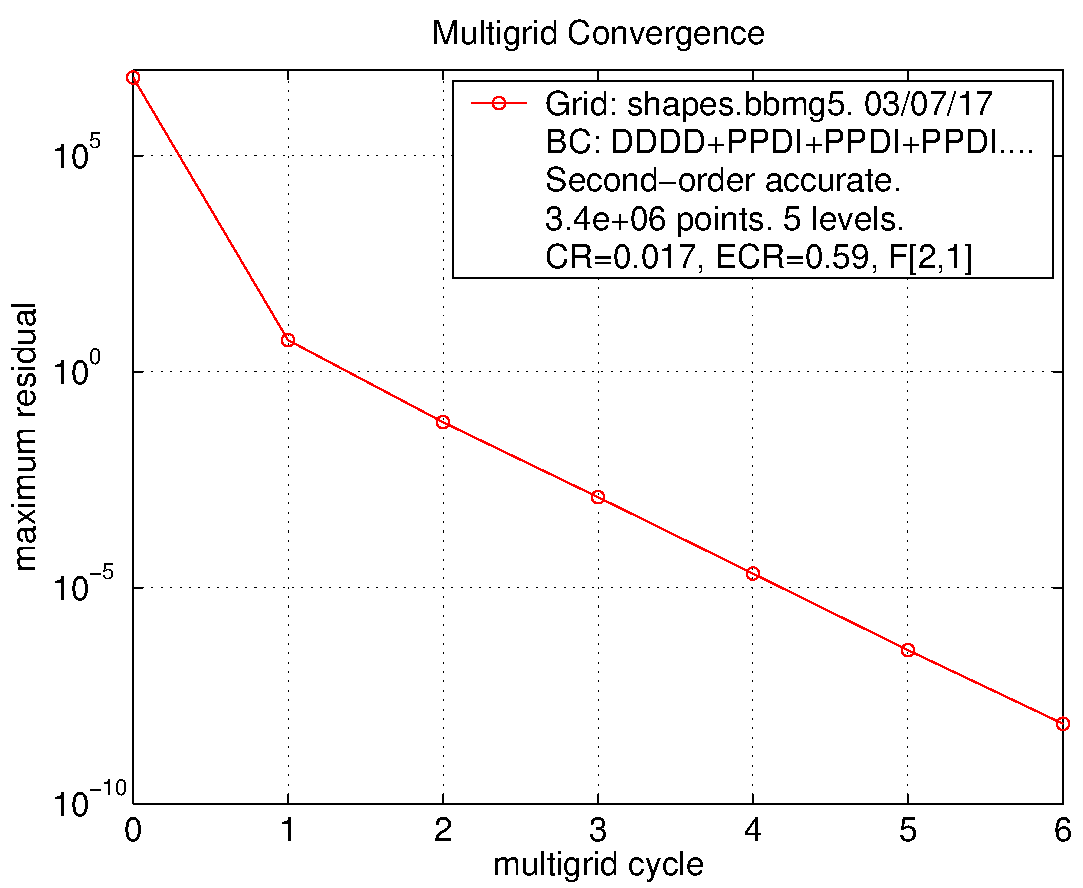
\includegraphics[width=.475\linewidth]{fig/residual_shapes_bbmg5_fmg}
  \end{center} 
\caption{Convergence history for shapes with FMG.}
\label{fig:shapes.bbmg5}
\end{figure}


\begin{table}[hbt]
\begin{center}
{\tablefontsize
\begin{tabular}{|c|c|c|c|c|} \hline 
 $i$   & $\vert\vert\mbox{res}\vert\vert_\infty$  &  CR     &  WU    & ECR  \\   \hline 
 $ 1$  & $ 5.2e+00$ & $0.000$ & $10.5$ & $0.26$ \\ 
 $ 2$  & $ 6.4e-02$ & $0.012$ & $ 6.6$ & $0.51$ \\ 
 $ 3$  & $ 1.0e-03$ & $0.016$ & $ 6.6$ & $0.54$ \\ 
 $ 4$  & $ 1.7e-05$ & $0.017$ & $ 6.8$ & $0.55$ \\ 
 $ 5$  & $ 2.8e-07$ & $0.016$ & $ 7.4$ & $0.58$ \\ 
\hline 
\multicolumn{5}{|c|}{Grid: shapes.bbmg5. 03/07/20}  \\
\multicolumn{5}{|c|}{BC: DDDD+PPDI+PPDI+PPDI....}  \\
\multicolumn{5}{|c|}{Second-order accurate.}  \\
\multicolumn{5}{|c|}{Trigonometric solution.}  \\
\multicolumn{5}{|c|}{Full Multigrid.}  \\
\multicolumn{5}{|c|}{F[2,1]: rb $\omega=1.10$, lz2 $\omega=1.00$}  \\
\multicolumn{5}{|c|}{3.40e+06 grid-points. 5 levels.}  \\
\multicolumn{5}{|c|}{Average CR=$0.015$, ECR=$0.54$.}  \\
\multicolumn{5}{|c|}{time/cycle = 3.40e+00 s.}  \\
\hline 
\end{tabular}
\begin{tabular}{|c|c|c|c|c|} \hline 
 $i$   & $\vert\vert\mbox{res}\vert\vert_\infty$  &  CR     &  WU    & ECR  \\   \hline 
 $ 1$  & $ 1.4e+01$ & $0.000$ & $ 7.8$ & $0.19$ \\ 
 $ 2$  & $ 3.5e-01$ & $0.025$ & $ 5.3$ & $0.50$ \\ 
 $ 3$  & $ 7.5e-03$ & $0.021$ & $ 5.2$ & $0.48$ \\ 
 $ 4$  & $ 1.2e-04$ & $0.016$ & $ 5.1$ & $0.44$ \\ 
 $ 5$  & $ 3.1e-06$ & $0.026$ & $ 5.2$ & $0.50$ \\ 
 $ 6$  & $ 9.5e-08$ & $0.031$ & $ 5.3$ & $0.52$ \\ 
\hline 
\multicolumn{5}{|c|}{Grid: shapes.bbmg5. 03/07/19}  \\
\multicolumn{5}{|c|}{BC: DDDD+PPDI+PPDI+PPDI....}  \\
\multicolumn{5}{|c|}{Second-order accurate.}  \\
\multicolumn{5}{|c|}{Trigonometric solution.}  \\
\multicolumn{5}{|c|}{Full Multigrid.}  \\
\multicolumn{5}{|c|}{F[1,1]: rb $\omega=1.10$, lz2 $\omega=1.00$}  \\
\multicolumn{5}{|c|}{3.40e+06 grid-points. 5 levels.}  \\
\multicolumn{5}{|c|}{Average CR=$0.023$, ECR=$0.49$.}  \\
\multicolumn{5}{|c|}{time/cycle = 2.59e+00 s.}  \\
\hline 
\end{tabular}
\begin{tabular}{|c|c|c|c|c|} \hline 
 $i$   & $\vert\vert\mbox{res}\vert\vert_\infty$  &  CR     &  WU    & ECR  \\   \hline 
 $ 1$  & $ 5.4e+00$ & $0.000$ & $13.3$ & $0.35$ \\ 
 $ 2$  & $ 6.8e-02$ & $0.013$ & $ 7.7$ & $0.57$ \\ 
 $ 3$  & $ 1.3e-03$ & $0.018$ & $ 7.7$ & $0.59$ \\ 
 $ 4$  & $ 2.1e-05$ & $0.017$ & $ 7.7$ & $0.59$ \\ 
 $ 5$  & $ 3.6e-07$ & $0.017$ & $ 7.6$ & $0.58$ \\ 
\hline 
\multicolumn{5}{|c|}{Grid: shapes.bbmg5. 03/07/13}  \\
\multicolumn{5}{|c|}{BC: DDDD+PPDI+PPDI+PPDI....}  \\
\multicolumn{5}{|c|}{Second-order accurate.}  \\
\multicolumn{5}{|c|}{Trigonometric solution.}  \\
\multicolumn{5}{|c|}{Full Multigrid.}  \\
\multicolumn{5}{|c|}{F[2,1]: rb $\omega=1.10$, lz2 $\omega=1.00$}  \\
\multicolumn{5}{|c|}{3.40e+06 grid-points. 5 levels.}  \\
\multicolumn{5}{|c|}{Average CR=$0.002$, ECR=$0.50$.}  \\
\multicolumn{5}{|c|}{time/cycle = 3.68e+00 s.}  \\
\hline 
\end{tabular}
\begin{tabular}{|c|c|c|c|c|} \hline 
 $i$   & $\vert\vert\mbox{res}\vert\vert_\infty$  &  CR     &  WU    & ECR  \\   \hline 
 $ 1$  & $ 7.4e+03$ & $0.001$ & $11.1$ & $0.54$ \\ 
 $ 2$  & $ 4.3e+01$ & $0.006$ & $ 7.6$ & $0.51$ \\ 
 $ 3$  & $ 6.7e-01$ & $0.016$ & $ 7.2$ & $0.56$ \\ 
 $ 4$  & $ 3.7e-02$ & $0.054$ & $ 7.1$ & $0.67$ \\ 
 $ 5$  & $ 5.8e-04$ & $0.016$ & $ 7.4$ & $0.57$ \\ 
 $ 6$  & $ 6.4e-06$ & $0.011$ & $ 7.5$ & $0.55$ \\ 
 $ 7$  & $ 1.3e-07$ & $0.021$ & $ 7.8$ & $0.61$ \\ 
\hline 
\multicolumn{5}{|c|}{Grid: shapes.bbmg5. 03/07/13}  \\
\multicolumn{5}{|c|}{BC: DDDD+PPDI+PPDI+PPDI....}  \\
\multicolumn{5}{|c|}{Second-order accurate.}  \\
\multicolumn{5}{|c|}{Trigonometric solution.}  \\
\multicolumn{5}{|c|}{F[2,1]: rb $\omega=1.10$, lz2 $\omega=1.00$}  \\
\multicolumn{5}{|c|}{3.40e+06 grid-points. 5 levels.}  \\
\multicolumn{5}{|c|}{Average CR=$0.011$, ECR=$0.57$.}  \\
\multicolumn{5}{|c|}{time/cycle = 3.17e+00 s.}  \\
\hline 
\end{tabular}
\begin{tabular}{|c|c|c|c|c|} \hline 
 $i$   & $\vert\vert\mbox{res}\vert\vert_\infty$  &  CR     &  WU    & ECR  \\   \hline 
 $ 1$  & $ 7.4e+03$ & $0.001$ & $16.1$ & $0.66$ \\ 
 $ 2$  & $ 5.8e+01$ & $0.008$ & $11.5$ & $0.66$ \\ 
 $ 3$  & $ 9.2e-01$ & $0.016$ & $11.3$ & $0.69$ \\ 
 $ 4$  & $ 1.6e-02$ & $0.018$ & $11.3$ & $0.70$ \\ 
 $ 5$  & $ 2.4e-04$ & $0.015$ & $11.4$ & $0.69$ \\ 
 $ 6$  & $ 2.6e-06$ & $0.011$ & $11.5$ & $0.68$ \\ 
 $ 7$  & $ 4.4e-08$ & $0.017$ & $11.6$ & $0.70$ \\ 
\hline 
\multicolumn{5}{|c|}{Grid: shapes.bbmg5. 03/07/13}  \\
\multicolumn{5}{|c|}{BC: DDDD+PPDI+PPDI+PPDI....}  \\
\multicolumn{5}{|c|}{Second-order accurate.}  \\
\multicolumn{5}{|c|}{Trigonometric solution.}  \\
\multicolumn{5}{|c|}{F[2,1]: rb $\omega=1.10$, lz2 $\omega=1.00$}  \\
\multicolumn{5}{|c|}{3.40e+06 grid-points. 5 levels.}  \\
\multicolumn{5}{|c|}{Average CR=$0.009$, ECR=$0.68$.}  \\
\multicolumn{5}{|c|}{time/cycle = 3.60e+00 s.}  \\
\hline 
\end{tabular}
\begin{tabular}{|c|c|c|c|c|} \hline 
 $i$   & $\vert\vert\mbox{res}\vert\vert_\infty$  &  CR     &  WU    & ECR  \\   \hline 
 $ 1$  & $ 1.0e+01$ & $0.005$ & $ 6.8$ & $0.46$ \\ 
 $ 2$  & $ 1.3e-01$ & $0.013$ & $ 6.4$ & $0.51$ \\ 
 $ 3$  & $ 2.0e-03$ & $0.016$ & $ 6.4$ & $0.52$ \\ 
 $ 4$  & $ 3.2e-05$ & $0.016$ & $ 6.5$ & $0.53$ \\ 
 $ 5$  & $ 4.7e-07$ & $0.015$ & $ 6.7$ & $0.53$ \\ 
 $ 6$  & $ 1.1e-08$ & $0.023$ & $ 6.8$ & $0.57$ \\ 
\hline 
\multicolumn{5}{|c|}{Grid: shapes.bbmg5. 03/06/18}  \\
\multicolumn{5}{|c|}{BC: DDDD+PPDI+PPDI+PPDI....}  \\
\multicolumn{5}{|c|}{Second-order accurate.}  \\
\multicolumn{5}{|c|}{Trigonometric solution. IBS-2-4-2}  \\
\multicolumn{5}{|c|}{W[2,1]: rb $\omega=1.10$, lz2 $\omega=1.00$}  \\
\multicolumn{5}{|c|}{3.40e+06 grid-points. 5 levels.}  \\
\multicolumn{5}{|c|}{Average CR=$0.013$, ECR=$0.52$.}  \\
\multicolumn{5}{|c|}{time/cycle = 4.73e+00 s.}  \\
\hline 
\end{tabular}
\begin{tabular}{|c|c|c|c|c|} \hline 
 $i$   & $\vert\vert\mbox{res}\vert\vert_\infty$  &  CR     &  WU    & ECR  \\   \hline 
 $ 1$  & $ 1.1e+02$ & $0.027$ & $ 7.0$ & $0.60$ \\ 
 $ 2$  & $ 3.1e+00$ & $0.029$ & $ 6.7$ & $0.59$ \\ 
 $ 3$  & $ 3.7e-01$ & $0.117$ & $ 6.2$ & $0.71$ \\ 
 $ 4$  & $ 9.8e-03$ & $0.027$ & $ 6.1$ & $0.55$ \\ 
 $ 5$  & $ 1.2e-03$ & $0.122$ & $ 6.1$ & $0.71$ \\ 
 $ 6$  & $ 3.3e-05$ & $0.027$ & $ 6.1$ & $0.55$ \\ 
 $ 7$  & $ 4.1e-06$ & $0.125$ & $ 6.1$ & $0.71$ \\ 
\hline 
\multicolumn{5}{|c|}{Grid: shapes.bbmg5. 03/06/18}  \\
\multicolumn{5}{|c|}{BC: DDDD+PPDI+PPDI+PPDI....}  \\
\multicolumn{5}{|c|}{Second-order accurate.}  \\
\multicolumn{5}{|c|}{Trigonometric solution.}  \\
\multicolumn{5}{|c|}{W[2,1]: rb $\omega=1.18$}  \\
\multicolumn{5}{|c|}{3.40e+06 grid-points. 5 levels.}  \\
\multicolumn{5}{|c|}{Average CR=$0.052$, ECR=$0.63$.}  \\
\multicolumn{5}{|c|}{time/cycle = 4.37e+00 s.}  \\
\hline 
\end{tabular}
\begin{tabular}{|c|c|c|c|c|} \hline 
 $i$   & $\vert\vert\mbox{res}\vert\vert_\infty$  &  CR     &  WU    & ECR  \\   \hline 
 $ 1$  & $ 4.3e+00$ & $0.010$ & $ 6.8$ & $0.51$ \\ 
 $ 2$  & $ 6.1e-02$ & $0.014$ & $ 6.7$ & $0.53$ \\ 
 $ 3$  & $ 9.0e-04$ & $0.015$ & $ 6.6$ & $0.53$ \\ 
 $ 4$  & $ 1.1e-05$ & $0.012$ & $ 6.7$ & $0.52$ \\ 
 $ 5$  & $ 2.4e-07$ & $0.023$ & $ 6.8$ & $0.57$ \\ 
 $ 6$  & $ 5.5e-09$ & $0.023$ & $ 6.8$ & $0.57$ \\ 
\hline 
\multicolumn{5}{|c|}{Grid: shapes.bbmg4. 03/06/18}  \\
\multicolumn{5}{|c|}{BC: DDDD+PPDI+PPDI+PPDI....}  \\
\multicolumn{5}{|c|}{Second-order accurate.}  \\
\multicolumn{5}{|c|}{Trigonometric solution.}  \\
\multicolumn{5}{|c|}{W[2,1]: rb $\omega=1.10$, lz2 $\omega=1.00$}  \\
\multicolumn{5}{|c|}{8.63e+05 grid-points. 4 levels.}  \\
\multicolumn{5}{|c|}{Average CR=$0.015$, ECR=$0.54$.}  \\
\multicolumn{5}{|c|}{time/cycle = 1.47e+00 s.}  \\
\hline 
\end{tabular}
\begin{tabular}{|c|c|c|c|c|} \hline 
 $i$   & $\vert\vert\mbox{res}\vert\vert_\infty$  &  CR     &  WU    & ECR  \\   \hline 
 $ 1$  & $ 1.6e+01$ & $0.013$ & $ 6.2$ & $0.50$ \\ 
 $ 2$  & $ 2.3e-01$ & $0.014$ & $ 6.3$ & $0.50$ \\ 
 $ 3$  & $ 4.6e-03$ & $0.020$ & $ 6.4$ & $0.54$ \\ 
 $ 4$  & $ 1.0e-04$ & $0.022$ & $ 6.7$ & $0.56$ \\ 
 $ 5$  & $ 9.4e-07$ & $0.009$ & $ 6.9$ & $0.51$ \\ 
 $ 6$  & $ 9.7e-09$ & $0.010$ & $ 6.9$ & $0.52$ \\ 
\hline 
\multicolumn{5}{|c|}{Grid: shapes.bbmg5. 03/06/18}  \\
\multicolumn{5}{|c|}{BC: DDDD+PPDI+PPDI+PPDI....}  \\
\multicolumn{5}{|c|}{Second-order accurate.}  \\
\multicolumn{5}{|c|}{Trigonometric solution. IBS+PBS}  \\
\multicolumn{5}{|c|}{W[2,1]: rb $\omega=1.10$, alz $\omega=1.00$}  \\
\multicolumn{5}{|c|}{3.40e+06 grid-points. 5 levels.}  \\
\multicolumn{5}{|c|}{Average CR=$0.014$, ECR=$0.52$.}  \\
\multicolumn{5}{|c|}{time/cycle = 4.54e+00 s.}  \\
\hline 
\end{tabular}
\begin{tabular}{|c|c|c|c|c|} \hline 
 $i$   & $\vert\vert\mbox{res}\vert\vert_\infty$  &  CR     &  WU    & ECR  \\   \hline 
 $ 1$  & $ 3.0e+01$ & $0.005$ & $ 7.0$ & $0.46$ \\ 
 $ 2$  & $ 1.5e+00$ & $0.050$ & $ 6.5$ & $0.63$ \\ 
 $ 3$  & $ 4.8e-02$ & $0.032$ & $ 6.3$ & $0.58$ \\ 
 $ 4$  & $ 2.5e-03$ & $0.052$ & $ 6.5$ & $0.63$ \\ 
 $ 5$  & $ 8.9e-05$ & $0.036$ & $ 6.9$ & $0.62$ \\ 
 $ 6$  & $ 5.0e-06$ & $0.057$ & $ 7.1$ & $0.67$ \\ 
 $ 7$  & $ 1.9e-07$ & $0.037$ & $ 7.1$ & $0.63$ \\ 
\hline 
\multicolumn{5}{|c|}{Grid: shapes.bbmg5. 03/06/13}  \\
\multicolumn{5}{|c|}{BC: DDDD+PPDI+PPDI+PPDI....}  \\
\multicolumn{5}{|c|}{Second-order accurate.}  \\
\multicolumn{5}{|c|}{Trigonometric solution.}  \\
\multicolumn{5}{|c|}{W[2,1]: rb $\omega=1.10$}  \\
\multicolumn{5}{|c|}{3.40e+06 grid-points. 5 levels.}  \\
\multicolumn{5}{|c|}{Average CR=$0.031$, ECR=$0.60$.}  \\
\multicolumn{5}{|c|}{time/cycle = 4.28e+00 s.}  \\
\hline 
\end{tabular}
} % \tablefontsize
\end{center}
\caption{Multigrid convergence rates for the shapes geometry.}
 \label{tab:shapesI} 
\end{table}



\begin{table}[hbt]
\begin{center}
{\tablefontsize
\begin{tabular}{|c|c|c|c|c|} \hline 
 $i$   & $\vert\vert\mbox{res}\vert\vert_\infty$  &  CR     &  WU    & ECR  \\   \hline 
 $ 1$  & $ 7.6e+01$ & $0.018$ & $ 7.1$ & $0.57$ \\ 
 $ 2$  & $ 1.5e+00$ & $0.019$ & $ 7.1$ & $0.58$ \\ 
 $ 3$  & $ 3.0e-02$ & $0.020$ & $ 7.1$ & $0.58$ \\ 
 $ 4$  & $ 6.1e-04$ & $0.021$ & $ 7.1$ & $0.58$ \\ 
 $ 5$  & $ 1.3e-05$ & $0.021$ & $ 7.1$ & $0.58$ \\ 
 $ 6$  & $ 2.7e-07$ & $0.021$ & $ 7.1$ & $0.58$ \\ 
 $ 7$  & $ 9.4e-09$ & $0.035$ & $ 7.1$ & $0.62$ \\ 
\hline 
\multicolumn{5}{|c|}{Grid: shapes.bbmg5. 03/06/13}  \\
\multicolumn{5}{|c|}{BC: DDDD+PPDI+PPDI+PPDI....}  \\
\multicolumn{5}{|c|}{Second-order accurate.}  \\
\multicolumn{5}{|c|}{Trigonometric solution.}  \\
\multicolumn{5}{|c|}{W[2,1]: rb $\omega=1.05$ FIX SS:1,7,4,4,4}  \\
\multicolumn{5}{|c|}{3.40e+06 grid-points. 5 levels.}  \\
\multicolumn{5}{|c|}{Average CR=$0.022$, ECR=$0.58$.}  \\
\multicolumn{5}{|c|}{time/cycle = 3.82e+00 s.}  \\
\hline 
\end{tabular}
\begin{tabular}{|c|c|c|c|c|} \hline 
 $i$   & $\vert\vert\mbox{res}\vert\vert_\infty$  &  CR     &  WU    & ECR  \\   \hline 
 $ 1$  & $ 7.6e+01$ & $0.015$ & $ 6.9$ & $0.54$ \\ 
 $ 2$  & $ 1.5e+00$ & $0.019$ & $ 6.9$ & $0.56$ \\ 
 $ 3$  & $ 3.0e-02$ & $0.020$ & $ 6.9$ & $0.57$ \\ 
 $ 4$  & $ 6.1e-04$ & $0.021$ & $ 6.9$ & $0.57$ \\ 
 $ 5$  & $ 1.8e-05$ & $0.030$ & $ 6.9$ & $0.60$ \\ 
 $ 6$  & $ 6.8e-07$ & $0.037$ & $ 6.9$ & $0.62$ \\ 
 $ 7$  & $ 7.0e-08$ & $0.103$ & $ 6.9$ & $0.72$ \\ 
\hline 
\multicolumn{5}{|c|}{Grid: shapes.bbmg5. 03/06/13}  \\
\multicolumn{5}{|c|}{BC: DDDD+PPDI+PPDI+PPDI....}  \\
\multicolumn{5}{|c|}{Second-order accurate.}  \\
\multicolumn{5}{|c|}{Trigonometric solution.}  \\
\multicolumn{5}{|c|}{W[2,1]: rb $\omega=1.05$ FIXED SUBSM}  \\
\multicolumn{5}{|c|}{3.40e+06 grid-points. 5 levels.}  \\
\multicolumn{5}{|c|}{Average CR=$0.028$, ECR=$0.60$.}  \\
\multicolumn{5}{|c|}{time/cycle = 3.56e+00 s.}  \\
\hline 
\end{tabular}
\begin{tabular}{|c|c|c|c|c|} \hline 
 $i$   & $\vert\vert\mbox{res}\vert\vert_\infty$  &  CR     &  WU    & ECR  \\   \hline 
 $ 1$  & $ 1.1e+02$ & $0.016$ & $ 6.5$ & $0.53$ \\ 
 $ 2$  & $ 2.6e+00$ & $0.023$ & $ 6.2$ & $0.54$ \\ 
 $ 3$  & $ 1.7e-01$ & $0.065$ & $ 6.3$ & $0.65$ \\ 
 $ 4$  & $ 2.6e-03$ & $0.015$ & $ 6.8$ & $0.54$ \\ 
 $ 5$  & $ 6.4e-05$ & $0.025$ & $ 7.1$ & $0.59$ \\ 
 $ 6$  & $ 1.3e-06$ & $0.021$ & $ 6.9$ & $0.57$ \\ 
 $ 7$  & $ 1.2e-07$ & $0.092$ & $ 6.9$ & $0.71$ \\ 
\hline 
\multicolumn{5}{|c|}{Grid: shapes.bbmg5. 03/06/13}  \\
\multicolumn{5}{|c|}{BC: DDDD+PPDI+PPDI+PPDI....}  \\
\multicolumn{5}{|c|}{Second-order accurate.}  \\
\multicolumn{5}{|c|}{Trigonometric solution.}  \\
\multicolumn{5}{|c|}{W[2,1]: rb $\omega=1.03$}  \\
\multicolumn{5}{|c|}{3.40e+06 grid-points. 5 levels.}  \\
\multicolumn{5}{|c|}{Average CR=$0.029$, ECR=$0.59$.}  \\
\multicolumn{5}{|c|}{time/cycle = 4.34e+00 s.}  \\
\hline 
\end{tabular}
\begin{tabular}{|c|c|c|c|c|} \hline 
 $i$   & $\vert\vert\mbox{res}\vert\vert_\infty$  &  CR     &  WU    & ECR  \\   \hline 
 $ 1$  & $ 1.1e+02$ & $0.011$ & $ 6.8$ & $0.51$ \\ 
 $ 2$  & $ 2.6e+00$ & $0.023$ & $ 6.3$ & $0.55$ \\ 
 $ 3$  & $ 8.2e-02$ & $0.031$ & $ 6.3$ & $0.58$ \\ 
 $ 4$  & $ 7.4e-03$ & $0.090$ & $ 6.6$ & $0.70$ \\ 
 $ 5$  & $ 3.7e-04$ & $0.050$ & $ 6.8$ & $0.64$ \\ 
 $ 6$  & $ 9.0e-06$ & $0.024$ & $ 6.8$ & $0.58$ \\ 
 $ 7$  & $ 1.5e-07$ & $0.016$ & $ 7.1$ & $0.56$ \\ 
\hline 
\multicolumn{5}{|c|}{Grid: shapes.bbmg5. 03/06/13}  \\
\multicolumn{5}{|c|}{BC: DDDD+PPDI+PPDI+PPDI....}  \\
\multicolumn{5}{|c|}{Second-order accurate.}  \\
\multicolumn{5}{|c|}{Trigonometric solution.}  \\
\multicolumn{5}{|c|}{W[2,1]: rb $\omega=1.03$}  \\
\multicolumn{5}{|c|}{3.40e+06 grid-points. 5 levels.}  \\
\multicolumn{5}{|c|}{Average CR=$0.028$, ECR=$0.59$.}  \\
\multicolumn{5}{|c|}{time/cycle = 4.16e+00 s.}  \\
\hline 
\end{tabular}
\begin{tabular}{|c|c|c|c|c|} \hline 
 $i$   & $\vert\vert\mbox{res}\vert\vert_\infty$  &  CR     &  WU    & ECR  \\   \hline 
 $ 1$  & $ 4.8e+01$ & $0.006$ & $ 6.9$ & $0.47$ \\ 
 $ 2$  & $ 1.4e+00$ & $0.029$ & $ 6.3$ & $0.57$ \\ 
 $ 3$  & $ 4.2e-02$ & $0.029$ & $ 6.3$ & $0.57$ \\ 
 $ 4$  & $ 2.4e-03$ & $0.057$ & $ 6.6$ & $0.65$ \\ 
 $ 5$  & $ 8.1e-05$ & $0.034$ & $ 6.9$ & $0.61$ \\ 
 $ 6$  & $ 4.8e-06$ & $0.059$ & $ 7.1$ & $0.67$ \\ 
 $ 7$  & $ 1.6e-07$ & $0.033$ & $ 7.4$ & $0.63$ \\ 
\hline 
\multicolumn{5}{|c|}{Grid: shapes.bbmg5. 03/06/13}  \\
\multicolumn{5}{|c|}{BC: DDDD+PPDI+PPDI+PPDI....}  \\
\multicolumn{5}{|c|}{Second-order accurate.}  \\
\multicolumn{5}{|c|}{Trigonometric solution.}  \\
\multicolumn{5}{|c|}{W[2,1]: rb $\omega=1.07$}  \\
\multicolumn{5}{|c|}{3.40e+06 grid-points. 5 levels.}  \\
\multicolumn{5}{|c|}{Average CR=$0.030$, ECR=$0.59$.}  \\
\multicolumn{5}{|c|}{time/cycle = 4.26e+00 s.}  \\
\hline 
\end{tabular}
\begin{tabular}{|c|c|c|c|c|} \hline 
 $i$   & $\vert\vert\mbox{res}\vert\vert_\infty$  &  CR     &  WU    & ECR  \\   \hline 
 $ 1$  & $ 3.0e+01$ & $0.005$ & $ 7.0$ & $0.46$ \\ 
 $ 2$  & $ 1.5e+00$ & $0.050$ & $ 6.5$ & $0.63$ \\ 
 $ 3$  & $ 4.8e-02$ & $0.032$ & $ 6.3$ & $0.58$ \\ 
 $ 4$  & $ 2.5e-03$ & $0.052$ & $ 6.5$ & $0.63$ \\ 
 $ 5$  & $ 8.9e-05$ & $0.036$ & $ 6.9$ & $0.62$ \\ 
 $ 6$  & $ 5.0e-06$ & $0.057$ & $ 7.1$ & $0.67$ \\ 
 $ 7$  & $ 1.9e-07$ & $0.037$ & $ 7.1$ & $0.63$ \\ 
\hline 
\multicolumn{5}{|c|}{Grid: shapes.bbmg5. 03/06/13}  \\
\multicolumn{5}{|c|}{BC: DDDD+PPDI+PPDI+PPDI....}  \\
\multicolumn{5}{|c|}{Second-order accurate.}  \\
\multicolumn{5}{|c|}{Trigonometric solution.}  \\
\multicolumn{5}{|c|}{W[2,1]: rb $\omega=1.10$}  \\
\multicolumn{5}{|c|}{3.40e+06 grid-points. 5 levels.}  \\
\multicolumn{5}{|c|}{Average CR=$0.031$, ECR=$0.60$.}  \\
\multicolumn{5}{|c|}{time/cycle = 4.28e+00 s.}  \\
\hline 
\end{tabular}
\begin{tabular}{|c|c|c|c|c|} \hline 
 $i$   & $\vert\vert\mbox{res}\vert\vert_\infty$  &  CR     &  WU    & ECR  \\   \hline 
 $ 1$  & $ 5.8e+01$ & $0.008$ & $ 6.5$ & $0.48$ \\ 
 $ 2$  & $ 2.3e+00$ & $0.040$ & $ 6.5$ & $0.61$ \\ 
 $ 3$  & $ 6.6e-02$ & $0.028$ & $ 6.3$ & $0.57$ \\ 
 $ 4$  & $ 3.8e-03$ & $0.058$ & $ 6.4$ & $0.64$ \\ 
 $ 5$  & $ 1.1e-04$ & $0.030$ & $ 6.4$ & $0.58$ \\ 
 $ 6$  & $ 6.4e-06$ & $0.057$ & $ 6.5$ & $0.64$ \\ 
 $ 7$  & $ 2.1e-07$ & $0.033$ & $ 6.6$ & $0.59$ \\ 
\hline 
\multicolumn{5}{|c|}{Grid: shapes.bbmg5. 03/06/13}  \\
\multicolumn{5}{|c|}{BC: DDDD+PPDI+PPDI+PPDI....}  \\
\multicolumn{5}{|c|}{Second-order accurate.}  \\
\multicolumn{5}{|c|}{Trigonometric solution.}  \\
\multicolumn{5}{|c|}{W[2,1]: rb $\omega=1.10$, lz2 $\omega=1.00$}  \\
\multicolumn{5}{|c|}{3.40e+06 grid-points. 5 levels.}  \\
\multicolumn{5}{|c|}{Average CR=$0.031$, ECR=$0.58$.}  \\
\multicolumn{5}{|c|}{time/cycle = 4.24e+00 s.}  \\
\hline 
\end{tabular}
\begin{tabular}{|c|c|c|c|c|} \hline 
 $i$   & $\vert\vert\mbox{res}\vert\vert_\infty$  &  CR     &  WU    & ECR  \\   \hline 
 $ 1$  & $ 1.9e+02$ & $0.016$ & $ 6.8$ & $0.54$ \\ 
 $ 2$  & $ 5.7e+00$ & $0.030$ & $ 6.3$ & $0.57$ \\ 
 $ 3$  & $ 1.9e-01$ & $0.033$ & $ 6.3$ & $0.58$ \\ 
 $ 4$  & $ 1.2e-02$ & $0.062$ & $ 6.6$ & $0.66$ \\ 
 $ 5$  & $ 5.3e-04$ & $0.045$ & $ 6.8$ & $0.63$ \\ 
 $ 6$  & $ 1.5e-05$ & $0.029$ & $ 6.8$ & $0.59$ \\ 
 $ 7$  & $ 6.9e-07$ & $0.046$ & $ 7.0$ & $0.64$ \\ 
\hline 
\multicolumn{5}{|c|}{Grid: shapes.bbmg5. 03/06/13}  \\
\multicolumn{5}{|c|}{BC: DDDD+PPDI+PPDI+PPDI....}  \\
\multicolumn{5}{|c|}{Second-order accurate.}  \\
\multicolumn{5}{|c|}{Trigonometric solution.}  \\
\multicolumn{5}{|c|}{W[2,1]: rb $\omega=1.00$}  \\
\multicolumn{5}{|c|}{3.40e+06 grid-points. 5 levels.}  \\
\multicolumn{5}{|c|}{Average CR=$0.034$, ECR=$0.60$.}  \\
\multicolumn{5}{|c|}{time/cycle = 4.20e+00 s.}  \\
\hline 
\end{tabular}
\begin{tabular}{|c|c|c|c|c|} \hline 
 $i$   & res      & rate    &  WU    & ECR  \\   \hline 
 $ 1$  & $ 1.2e+01$ & $0.030$ & $ 6.1$ & $0.56$ \\ 
 $ 2$  & $ 2.3e-01$ & $0.019$ & $ 5.4$ & $0.48$ \\ 
 $ 3$  & $ 1.6e-02$ & $0.069$ & $ 6.6$ & $0.67$ \\ 
 $ 4$  & $ 9.9e-04$ & $0.063$ & $ 6.0$ & $0.63$ \\ 
 $ 5$  & $ 6.6e-05$ & $0.067$ & $ 5.7$ & $0.62$ \\ 
 $ 6$  & $ 4.7e-06$ & $0.072$ & $ 6.8$ & $0.68$ \\ 
 $ 7$  & $ 3.2e-07$ & $0.069$ & $ 7.2$ & $0.69$ \\ 
%  $ 8$  & $ 2.1e-08$ & $0.066$ & $ 6.7$ & $0.67$ \\ 
%  $ 9$  & $ 1.4e-09$ & $0.066$ & $ 6.1$ & $0.64$ \\ 
\hline 
\multicolumn{5}{|c|}{Grid: shapes.bbmg2.}  \\
\multicolumn{5}{|c|}{Dirichlet boundary conditions.}  \\
\multicolumn{5}{|c|}{Second-order accurate.}  \\
\multicolumn{5}{|c|}{Trigonometric solution.}  \\
\multicolumn{5}{|c|}{Smoother rb[2,1] $\omega=1.10$}  \\
\multicolumn{5}{|c|}{6.85e+04 grid-points. 4 levels.}  \\
\multicolumn{5}{|c|}{Average CR=$0.053$, ECR=$0.63$.}  \\
\multicolumn{5}{|c|}{time/cycle = 1.19e-01 s.}  \\
\hline 
\end{tabular}
% \qquad % --------------------------------------------------------------------
\begin{tabular}{|c|c|c|c|c|} \hline 
 $i$   & res      & rate    &  WU    & ECR  \\   \hline 
 $ 1$  & $ 1.5e+02$ & $0.017$ & $ 5.6$ & $0.48$ \\ 
 $ 2$  & $ 1.3e+00$ & $0.008$ & $ 5.1$ & $0.40$ \\ 
 $ 3$  & $ 4.5e-02$ & $0.034$ & $ 5.5$ & $0.54$ \\ 
 $ 4$  & $ 2.3e-03$ & $0.050$ & $ 5.9$ & $0.60$ \\ 
 $ 5$  & $ 1.1e-04$ & $0.049$ & $ 5.9$ & $0.60$ \\ 
 $ 6$  & $ 7.0e-06$ & $0.063$ & $ 5.9$ & $0.62$ \\ 
 $ 7$  & $ 5.0e-07$ & $0.072$ & $ 5.9$ & $0.64$ \\ 
\hline 
\multicolumn{5}{|c|}{Grid: shapes.bbmg4.}  \\
\multicolumn{5}{|c|}{Dirichlet boundary conditions.}  \\
\multicolumn{5}{|c|}{Second-order accurate.}  \\
\multicolumn{5}{|c|}{Trigonometric solution.}  \\
\multicolumn{5}{|c|}{Smoother rb[2,1] $\omega=1.10$}  \\
\multicolumn{5}{|c|}{8.63e+05 grid-points. 4 levels.}  \\
\multicolumn{5}{|c|}{Average CR=$0.034$, ECR=$0.55$.}  \\
\multicolumn{5}{|c|}{time/cycle = 8.84e-01 s.}  \\
\hline 
\end{tabular}
%\qquad % --------------------------------------------------------------------
% \vskip\baselineskip
\begin{tabular}{|c|c|c|c|c|} \hline 
 $i$   & res      & rate    &  WU    & ECR  \\   \hline 
 $ 1$  & $ 6.2e+02$ & $0.015$ & $ 5.3$ & $0.46$ \\ 
 $ 2$  & $ 1.9e+01$ & $0.030$ & $ 5.2$ & $0.51$ \\ 
 $ 3$  & $ 1.3e+00$ & $0.068$ & $ 5.3$ & $0.60$ \\ 
 $ 4$  & $ 8.4e-02$ & $0.066$ & $ 5.3$ & $0.60$ \\ 
 $ 5$  & $ 5.5e-03$ & $0.065$ & $ 5.3$ & $0.60$ \\ 
 $ 6$  & $ 3.6e-04$ & $0.065$ & $ 5.3$ & $0.60$ \\ 
 $ 7$  & $ 2.3e-05$ & $0.066$ & $ 5.3$ & $0.60$ \\ 
%  $ 8$  & $ 1.5e-06$ & $0.065$ & $ 5.3$ & $0.60$ \\ 
%  $ 9$  & $ 1.1e-07$ & $0.075$ & $ 5.3$ & $0.62$ \\ 
\hline 
\multicolumn{5}{|c|}{Grid: shapes.bbmg5.}  \\
\multicolumn{5}{|c|}{Dirichlet boundary conditions.}  \\
\multicolumn{5}{|c|}{Second-order accurate.}  \\
\multicolumn{5}{|c|}{Trigonometric solution.}  \\
\multicolumn{5}{|c|}{Smoother rb[2,1] $\omega=1.10$}  \\
\multicolumn{5}{|c|}{3.30e+06 grid-points. 4 levels.}  \\
\multicolumn{5}{|c|}{Average CR=$0.052$, ECR=$0.57$.}  \\
\multicolumn{5}{|c|}{time/cycle = 2.79e+00 s.}  \\
\hline 
\end{tabular}
%\qquad % --------------------------------------------------------------------
% \begin{tabular}{|c|c|c|c|c|} \hline 
%  $i$   & res      & rate    &  WU    & ECR  \\   \hline 
%  $ 1$  & $ 6.2e+02$ & $0.025$ & $ 5.1$ & $0.49$ \\ 
%  $ 2$  & $ 1.4e+01$ & $0.022$ & $ 5.2$ & $0.48$ \\ 
%  $ 3$  & $ 8.8e-01$ & $0.064$ & $ 5.4$ & $0.60$ \\ 
%  $ 4$  & $ 7.5e-02$ & $0.085$ & $ 5.5$ & $0.64$ \\ 
%  $ 5$  & $ 5.8e-03$ & $0.077$ & $ 5.4$ & $0.62$ \\ 
%  $ 6$  & $ 4.6e-04$ & $0.080$ & $ 5.4$ & $0.63$ \\ 
%  $ 7$  & $ 3.6e-05$ & $0.078$ & $ 5.5$ & $0.63$ \\ 
%  $ 8$  & $ 2.8e-06$ & $0.079$ & $ 5.5$ & $0.63$ \\ 
%  $ 9$  & $ 2.2e-07$ & $0.079$ & $ 5.5$ & $0.63$ \\ 
% \hline 
% \multicolumn{5}{|c|}{Grid: shapes.bbmg5.}  \\
% \multicolumn{5}{|c|}{Dirichlet boundary conditions.}  \\
% \multicolumn{5}{|c|}{Second-order accurate.}  \\
% \multicolumn{5}{|c|}{Trigonometric solution.}  \\
% \multicolumn{5}{|c|}{Smoother rb[2,1] $\omega=1.10$, lz1[2,1] $\omega=1.00$}  \\
% \multicolumn{5}{|c|}{3.30e+06 grid-points. 4 levels.}  \\
% \multicolumn{5}{|c|}{Average CR=$0.059$, ECR=$0.59$.}  \\
% \multicolumn{5}{|c|}{time/cycle = 3.05e+00 s.}  \\
% \hline 
% \end{tabular}
} % \tablefontsize
\end{center}
\caption{Multigrid convergence rates for the shapes geometry.}
 \label{tab:shapesII} 
\end{table}







% ===================================================================================================
\clearpage
\subsection{Airfoils in a channel}

% ===================================================================================



{
\newcommand{\figWidth}{8.cm}
\newcommand{\trimfig}[2]{\trimPlotb{#1}{#2}{.0}{.0}{.2}{.2}}
\newcommand{\figWidtha}{7.cm}
\newcommand{\trimfiga}[2]{\trimPlotb{#1}{#2}{.0}{.0}{. }{.0}}
\begin{figure}[hbt]
\begin{center}
\begin{tikzpicture}[scale=1]
  \useasboundingbox (0,.7) rectangle (16.,13);  % set the bounding box (so we have less surrounding white space)
%
  \draw ( 0.0,6.25) node[anchor=south west,xshift=-4pt,yshift=+0pt] {\trimfig{fig/joukowsky_u}{\figWidth}};
  \draw ( 8.0,6.25) node[anchor=south west,xshift=-4pt,yshift=+0pt] {\trimfig{fig/joukowsky_level2}{\figWidth}};
%
%  \draw ( 0.0,0.0) node[anchor=south west,xshift=-4pt,yshift=+0pt] {\trimfig{fig/shapes_bbmg4_error}{\figWidth}};
  \draw ( 7.5,0.0) node[anchor=south west,xshift=-4pt,yshift=+0pt] {\trimfiga{fig/residual_joukowsky}{\figWidtha}};
%
 % \draw (current bounding box.south west) rectangle (current bounding box.north east);
% grid:
%\draw[step=1cm,gray] (0,0) grid (15,14);
\end{tikzpicture}
\end{center}
\caption{Top: computed solution for two airfoils in a channel.
Middle: The overlapping grid on level 3 (joukowsky). 
Bottom : convergence history.} \label{fig:joukowsky}
\end{figure}
}


\begin{table}[hbt]
\begin{center}
{\tablefontsize
\begin{tabular}{|c|c|c|c|c|} \hline 
 $i$   & $\vert\vert\mbox{res}\vert\vert_\infty$  &  CR     &  WU    & ECR  \\   \hline 
 $ 1$  & $ 7.2e-01$ & $0.011$ & $ 6.3$ & $0.49$ \\ 
 $ 2$  & $ 5.3e-03$ & $0.007$ & $ 6.3$ & $0.46$ \\ 
 $ 3$  & $ 1.1e-04$ & $0.020$ & $ 6.4$ & $0.54$ \\ 
 $ 4$  & $ 1.7e-06$ & $0.016$ & $ 6.6$ & $0.53$ \\ 
 $ 5$  & $ 3.5e-08$ & $0.021$ & $ 6.6$ & $0.56$ \\ 
 $ 6$  & $ 1.1e-09$ & $0.030$ & $ 6.6$ & $0.59$ \\ 
\hline 
\multicolumn{5}{|c|}{Grid: joukowsky. 03/06/18}  \\
\multicolumn{5}{|c|}{BC: DDDD+PPDI+PPDI.}  \\
\multicolumn{5}{|c|}{Second-order accurate.}  \\
\multicolumn{5}{|c|}{Trigonometric solution. IBS-2-4-2}  \\
\multicolumn{5}{|c|}{W[2,1]: rb $\omega=1.10$, alz $\omega=1.00$}  \\
\multicolumn{5}{|c|}{2.20e+06 grid-points. 4 levels.}  \\
\multicolumn{5}{|c|}{Average CR=$0.016$, ECR=$0.53$.}  \\
\multicolumn{5}{|c|}{time/cycle = 3.86e+00 s.}  \\
\hline 
\end{tabular}
\begin{tabular}{|c|c|c|c|c|} \hline 
 $i$   & $\vert\vert\mbox{res}\vert\vert_\infty$  &  CR     &  WU    & ECR  \\   \hline 
 $ 1$  & $ 2.8e-01$ & $0.005$ & $ 6.4$ & $0.44$ \\ 
 $ 2$  & $ 4.0e-03$ & $0.014$ & $ 6.4$ & $0.52$ \\ 
 $ 3$  & $ 9.8e-05$ & $0.024$ & $ 6.6$ & $0.57$ \\ 
 $ 4$  & $ 2.2e-06$ & $0.022$ & $ 6.6$ & $0.56$ \\ 
 $ 5$  & $ 5.3e-08$ & $0.025$ & $ 6.6$ & $0.57$ \\ 
 $ 6$  & $ 1.2e-09$ & $0.023$ & $ 6.6$ & $0.57$ \\ 
\hline 
\multicolumn{5}{|c|}{Grid: joukowsky. 03/06/18}  \\
\multicolumn{5}{|c|}{BC: DDDD+PPDI+PPDI.}  \\
\multicolumn{5}{|c|}{Second-order accurate.}  \\
\multicolumn{5}{|c|}{Trigonometric solution. IBS + PBS}  \\
\multicolumn{5}{|c|}{W[2,1]: rb $\omega=1.10$, alz $\omega=1.00$}  \\
\multicolumn{5}{|c|}{2.20e+06 grid-points. 4 levels.}  \\
\multicolumn{5}{|c|}{Average CR=$0.017$, ECR=$0.54$.}  \\
\multicolumn{5}{|c|}{time/cycle = 4.71e+00 s.}  \\
\hline 
\end{tabular}
\begin{tabular}{|c|c|c|c|c|} \hline 
 $i$   & res      & rate    &  WU    & ECR  \\   \hline 
 $ 1$  & $ 2.3e+02$ & $0.168$ & $ 5.6$ & $0.73$ \\ 
 $ 2$  & $ 1.4e+00$ & $0.006$ & $ 5.6$ & $0.40$ \\ 
 $ 3$  & $ 3.4e-01$ & $0.245$ & $ 5.6$ & $0.78$ \\ 
 $ 4$  & $ 9.8e-03$ & $0.029$ & $ 5.6$ & $0.53$ \\ 
 $ 5$  & $ 1.8e-03$ & $0.186$ & $ 5.6$ & $0.74$ \\ 
 $ 6$  & $ 1.9e-04$ & $0.104$ & $ 5.6$ & $0.67$ \\ 
 $ 7$  & $ 1.1e-05$ & $0.057$ & $ 5.6$ & $0.60$ \\ 
 $ 8$  & $ 7.3e-07$ & $0.069$ & $ 5.6$ & $0.62$ \\ 
\hline 
\multicolumn{5}{|c|}{Grid: joukowsky.}  \\
\multicolumn{5}{|c|}{BC: DDDD+PPDI+PPDI.}  \\
\multicolumn{5}{|c|}{Second-order accurate.}  \\
\multicolumn{5}{|c|}{Trigonometric solution.}  \\
\multicolumn{5}{|c|}{V[2,1]: rb $\omega=1.10$, alj $\omega=0.80$}  \\
\multicolumn{5}{|c|}{2.20e+06 grid-points. 4 levels.}  \\
\multicolumn{5}{|c|}{Average CR=$0.069$, ECR=$0.62$.}  \\
\multicolumn{5}{|c|}{time/cycle = 3.29e+00 s.}  \\
\hline 
\end{tabular}
\qquad
\begin{tabular}{|c|c|c|c|c|} \hline 
 $i$   & $\vert\vert\mbox{res}\vert\vert_\infty$  &  CR     &  WU    & ECR  \\   \hline 
 $ 1$  & $ 1.4e+01$ & $0.020$ & $ 6.6$ & $0.55$ \\ 
 $ 2$  & $ 3.7e-01$ & $0.025$ & $ 6.6$ & $0.57$ \\ 
 $ 3$  & $ 4.0e-02$ & $0.108$ & $ 6.6$ & $0.71$ \\ 
 $ 4$  & $ 4.2e-03$ & $0.105$ & $ 6.6$ & $0.71$ \\ 
 $ 5$  & $ 4.4e-04$ & $0.104$ & $ 6.6$ & $0.71$ \\ 
 $ 6$  & $ 4.5e-05$ & $0.103$ & $ 6.6$ & $0.71$ \\ 
 $ 7$  & $ 4.6e-06$ & $0.103$ & $ 6.6$ & $0.71$ \\ 
 $ 8$  & $ 5.7e-07$ & $0.124$ & $ 6.6$ & $0.73$ \\ 
\hline 
\multicolumn{5}{|c|}{Grid: joukowsky.}  \\
\multicolumn{5}{|c|}{BC: DDDD+PPDI+PPDI.}  \\
\multicolumn{5}{|c|}{Second-order accurate.}  \\
\multicolumn{5}{|c|}{Trigonometric solution.}  \\
\multicolumn{5}{|c|}{W[2,1]: rb $\omega=1.10$, lz2 $\omega=1.20$}  \\
\multicolumn{5}{|c|}{2.20e+06 grid-points. 4 levels.}  \\
\multicolumn{5}{|c|}{Average CR=$0.073$, ECR=$0.67$.}  \\
\multicolumn{5}{|c|}{time/cycle = 3.22e+00 s.}  \\
\hline 
\end{tabular}
\qquad
\begin{tabular}{|c|c|c|c|c|} \hline 
 $i$   & $\vert\vert\mbox{res}\vert\vert_\infty$  &  CR     &  WU    & ECR  \\   \hline 
 $ 1$  & $ 1.7e+01$ & $0.169$ & $ 6.6$ & $0.76$ \\ 
 $ 2$  & $ 2.1e-01$ & $0.012$ & $ 6.6$ & $0.51$ \\ 
 $ 3$  & $ 4.5e-02$ & $0.214$ & $ 6.6$ & $0.79$ \\ 
 $ 4$  & $ 2.1e-03$ & $0.048$ & $ 6.5$ & $0.63$ \\ 
 $ 5$  & $ 1.3e-04$ & $0.059$ & $ 6.5$ & $0.65$ \\ 
 $ 6$  & $ 1.0e-05$ & $0.079$ & $ 6.5$ & $0.68$ \\ 
 $ 7$  & $ 7.1e-07$ & $0.071$ & $ 6.5$ & $0.67$ \\ 
 $ 8$  & $ 6.6e-08$ & $0.093$ & $ 6.6$ & $0.70$ \\ 
\hline 
\multicolumn{5}{|c|}{Grid: joukowsky.}  \\
\multicolumn{5}{|c|}{BC: DDDD+PPDI+PPDI.}  \\
\multicolumn{5}{|c|}{Second-order accurate.}  \\
\multicolumn{5}{|c|}{Trigonometric solution.}  \\
\multicolumn{5}{|c|}{W[2,1]: rb $\omega=1.10$, alj $\omega=0.80$}  \\
\multicolumn{5}{|c|}{2.20e+06 grid-points. 4 levels.}  \\
\multicolumn{5}{|c|}{Average CR=$0.071$, ECR=$0.67$.}  \\
\multicolumn{5}{|c|}{time/cycle = 3.13e+00 s.}  \\
\hline 
\end{tabular}
} % \tablefontsize
\end{center}
\caption{Multigrid convergence rates for two airfoils in a channel.}
\label{fig:smoothBox}
\end{table}


\begin{table}[hbt]
\begin{center}
{\tablefontsize
\begin{tabular}{|c|c|c|c|c|} \hline 
 $i$   & $\vert\vert\mbox{res}\vert\vert_\infty$  &  CR     &  WU    & ECR  \\   \hline 
 $ 1$  & $ 2.3e+02$ & $0.045$ & $ 4.3$ & $0.48$ \\ 
 $ 2$  & $ 2.7e+01$ & $0.113$ & $ 4.2$ & $0.59$ \\ 
 $ 3$  & $ 3.4e+00$ & $0.129$ & $ 4.1$ & $0.60$ \\ 
 $ 4$  & $ 5.1e-01$ & $0.149$ & $ 4.0$ & $0.62$ \\ 
 $ 5$  & $ 7.9e-02$ & $0.154$ & $ 4.1$ & $0.63$ \\ 
 $ 6$  & $ 2.6e-02$ & $0.327$ & $ 4.1$ & $0.76$ \\ 
 $ 7$  & $ 1.9e-03$ & $0.074$ & $ 4.2$ & $0.54$ \\ 
 $ 8$  & $ 2.1e-04$ & $0.110$ & $ 4.2$ & $0.59$ \\ 
\hline 
\multicolumn{5}{|c|}{Grid: joukowsky. 03/06/08}  \\
\multicolumn{5}{|c|}{BC: DDDD+PPDI+PPDI.}  \\
\multicolumn{5}{|c|}{Second-order accurate.}  \\
\multicolumn{5}{|c|}{Trigonometric solution.}  \\
\multicolumn{5}{|c|}{V[1,1]: rb $\omega=1.45$}  \\
\multicolumn{5}{|c|}{2.20e+06 grid-points. 4 levels.}  \\
\multicolumn{5}{|c|}{Average CR=$0.119$, ECR=$0.60$.}  \\
\multicolumn{5}{|c|}{time/cycle = 2.06e+00 s.}  \\
\hline 
\end{tabular}
\begin{tabular}{|c|c|c|c|c|} \hline 
 $i$   & $\vert\vert\mbox{res}\vert\vert_\infty$  &  CR     &  WU    & ECR  \\   \hline 
 $ 1$  & $ 6.4e+01$ & $0.019$ & $ 5.2$ & $0.47$ \\ 
 $ 2$  & $ 5.0e+00$ & $0.078$ & $ 5.1$ & $0.61$ \\ 
 $ 3$  & $ 4.5e-01$ & $0.090$ & $ 5.0$ & $0.62$ \\ 
 $ 4$  & $ 3.5e-02$ & $0.078$ & $ 4.9$ & $0.59$ \\ 
 $ 5$  & $ 4.3e-03$ & $0.124$ & $ 4.9$ & $0.65$ \\ 
 $ 6$  & $ 6.1e-04$ & $0.140$ & $ 4.9$ & $0.67$ \\ 
 $ 7$  & $ 7.9e-05$ & $0.130$ & $ 5.0$ & $0.67$ \\ 
 $ 8$  & $ 1.3e-05$ & $0.161$ & $ 5.1$ & $0.70$ \\ 
\hline 
\multicolumn{5}{|c|}{Grid: joukowsky. 03/06/08}  \\
\multicolumn{5}{|c|}{BC: DDDD+PPDI+PPDI.}  \\
\multicolumn{5}{|c|}{Second-order accurate.}  \\
\multicolumn{5}{|c|}{Trigonometric solution.}  \\
\multicolumn{5}{|c|}{W[1,1]: rb $\omega=1.45$}  \\
\multicolumn{5}{|c|}{2.20e+06 grid-points. 4 levels.}  \\
\multicolumn{5}{|c|}{Average CR=$0.088$, ECR=$0.62$.}  \\
\multicolumn{5}{|c|}{time/cycle = 3.24e+00 s.}  \\
\hline 
\end{tabular}
\begin{tabular}{|c|c|c|c|c|} \hline 
 $i$   & $\vert\vert\mbox{res}\vert\vert_\infty$  &  CR     &  WU    & ECR  \\   \hline 
 $ 1$  & $ 9.4e+00$ & $0.035$ & $ 5.0$ & $0.51$ \\ 
 $ 2$  & $ 3.0e-01$ & $0.032$ & $ 4.9$ & $0.50$ \\ 
 $ 3$  & $ 3.6e-02$ & $0.121$ & $ 5.0$ & $0.65$ \\ 
 $ 4$  & $ 1.6e-03$ & $0.045$ & $ 5.1$ & $0.54$ \\ 
 $ 5$  & $ 2.7e-04$ & $0.168$ & $ 5.2$ & $0.71$ \\ 
 $ 6$  & $ 1.7e-05$ & $0.063$ & $ 5.2$ & $0.59$ \\ 
 $ 7$  & $ 2.0e-06$ & $0.116$ & $ 5.2$ & $0.66$ \\ 
 $ 8$  & $ 2.8e-07$ & $0.139$ & $ 5.2$ & $0.69$ \\ 
\hline 
\multicolumn{5}{|c|}{Grid: joukowsky. 03/06/08}  \\
\multicolumn{5}{|c|}{BC: DDDD+PPDI+PPDI.}  \\
\multicolumn{5}{|c|}{Second-order accurate.}  \\
\multicolumn{5}{|c|}{Trigonometric solution.}  \\
\multicolumn{5}{|c|}{W[1,1]: rb $\omega=1.10$, alz $\omega=1.00$}  \\
\multicolumn{5}{|c|}{2.20e+06 grid-points. 4 levels.}  \\
\multicolumn{5}{|c|}{Average CR=$0.075$, ECR=$0.60$.}  \\
\multicolumn{5}{|c|}{time/cycle = 2.81e+00 s.}  \\
\hline 
\end{tabular}
\begin{tabular}{|c|c|c|c|c|} \hline 
 $i$   & $\vert\vert\mbox{res}\vert\vert_\infty$  &  CR     &  WU    & ECR  \\   \hline 
 $ 1$  & $ 6.6e+01$ & $0.053$ & $ 4.9$ & $0.55$ \\ 
 $ 2$  & $ 3.7e+00$ & $0.056$ & $ 4.9$ & $0.56$ \\ 
 $ 3$  & $ 2.1e-01$ & $0.057$ & $ 4.9$ & $0.56$ \\ 
 $ 4$  & $ 1.2e-02$ & $0.057$ & $ 4.9$ & $0.56$ \\ 
 $ 5$  & $ 7.1e-04$ & $0.059$ & $ 4.9$ & $0.56$ \\ 
 $ 6$  & $ 4.1e-05$ & $0.058$ & $ 4.9$ & $0.56$ \\ 
 $ 7$  & $ 1.1e-05$ & $0.260$ & $ 5.0$ & $0.76$ \\ 
 $ 8$  & $ 5.5e-07$ & $0.052$ & $ 5.0$ & $0.55$ \\ 
\hline 
\multicolumn{5}{|c|}{Grid: joukowsky. 03/06/08}  \\
\multicolumn{5}{|c|}{BC: DDDD+PPDI+PPDI.}  \\
\multicolumn{5}{|c|}{Second-order accurate.}  \\
\multicolumn{5}{|c|}{Trigonometric solution.}  \\
\multicolumn{5}{|c|}{W[1,1]: rb $\omega=1.00$, alz $\omega=1.00$}  \\
\multicolumn{5}{|c|}{2.20e+06 grid-points. 4 levels.}  \\
\multicolumn{5}{|c|}{Average CR=$0.068$, ECR=$0.58$.}  \\
\multicolumn{5}{|c|}{time/cycle = 2.68e+00 s.}  \\
\hline 
\end{tabular}
} % \tablefontsize
\end{center}
\caption{Multigrid convergence rates for two airfoils in a channel.}
\label{fig:airfoils2}
\end{table}











% =================================================================================================
\clearpage
\subsection{Box}

\begin{table}[hbt]
\begin{center}
\tablefontsize
\begin{tabular}{|c|c|c|c|c|} \hline 
 $i$   & res      & rate    &  WU    & ECR  \\   \hline 
 $ 1$  & $ 3.7e+00$ & $0.023$ & $ 4.6$ & $0.44$ \\ 
 $ 2$  & $ 4.4e-02$ & $0.012$ & $ 4.6$ & $0.38$ \\ 
 $ 3$  & $ 8.3e-04$ & $0.019$ & $ 4.6$ & $0.43$ \\ 
 $ 4$  & $ 1.3e-05$ & $0.016$ & $ 4.6$ & $0.41$ \\ 
 $ 5$  & $ 2.4e-07$ & $0.018$ & $ 4.6$ & $0.42$ \\ 
 $ 6$  & $ 5.9e-09$ & $0.025$ & $ 4.6$ & $0.45$ \\ 
 $ 7$  & $ 1.3e-10$ & $0.023$ & $ 4.6$ & $0.44$ \\ 
\hline 
\multicolumn{5}{|c|}{Grid: box32.}  \\
\multicolumn{5}{|c|}{Dirichlet boundary conditions.}  \\
\multicolumn{5}{|c|}{Second-order accurate.}  \\
\multicolumn{5}{|c|}{Trigonometric solution.}  \\
\multicolumn{5}{|c|}{Smoother rb[2,1] $\omega=1.15$}  \\
\multicolumn{5}{|c|}{5.07e+04 grid-points. 5 levels.}  \\
\multicolumn{5}{|c|}{Average CR=$0.019$, ECR=$0.42$.}  \\
\multicolumn{5}{|c|}{time/cycle = 1.04e-01 s.}  \\
\hline 
\end{tabular}
\begin{tabular}{|c|c|c|c|c|} \hline 
 $i$   & res      & rate    &  WU    & ECR  \\   \hline 
 $ 1$  & $ 7.9e+01$ & $0.028$ & $ 4.6$ & $0.46$ \\ 
 $ 2$  & $ 1.5e+00$ & $0.019$ & $ 4.6$ & $0.42$ \\ 
 $ 3$  & $ 2.5e-02$ & $0.017$ & $ 4.6$ & $0.41$ \\ 
 $ 4$  & $ 5.1e-04$ & $0.021$ & $ 4.6$ & $0.43$ \\ 
 $ 5$  & $ 9.4e-06$ & $0.018$ & $ 4.6$ & $0.42$ \\ 
 $ 6$  & $ 1.6e-07$ & $0.017$ & $ 4.6$ & $0.41$ \\ 
 $ 7$  & $ 3.0e-09$ & $0.019$ & $ 4.6$ & $0.43$ \\ 
\hline 
\multicolumn{5}{|c|}{Grid: box128.}  \\
\multicolumn{5}{|c|}{Dirichlet boundary conditions.}  \\
\multicolumn{5}{|c|}{Second-order accurate.}  \\
\multicolumn{5}{|c|}{Trigonometric solution.}  \\
\multicolumn{5}{|c|}{Smoother rb[2,1] $\omega=1.15$}  \\
\multicolumn{5}{|c|}{2.35e+06 grid-points. 5 levels.}  \\
\multicolumn{5}{|c|}{Average CR=$0.019$, ECR=$0.43$.}  \\
\multicolumn{5}{|c|}{time/cycle = 2.07e+00 s.}  \\
\hline 
\end{tabular}
\begin{tabular}{|c|c|c|c|c|} \hline 
 $i$   & res      & rate    &  WU    & ECR  \\   \hline 
 $ 1$  & $ 2.8e+02$ & $0.054$ & $ 3.6$ & $0.44$ \\ 
 $ 2$  & $ 1.3e+01$ & $0.045$ & $ 3.6$ & $0.42$ \\ 
 $ 3$  & $ 7.3e-01$ & $0.057$ & $ 3.6$ & $0.45$ \\ 
 $ 4$  & $ 3.3e-02$ & $0.046$ & $ 3.6$ & $0.42$ \\ 
 $ 5$  & $ 1.5e-03$ & $0.044$ & $ 3.6$ & $0.42$ \\ 
 $ 6$  & $ 1.1e-04$ & $0.072$ & $ 3.6$ & $0.48$ \\ 
 $ 7$  & $ 6.6e-06$ & $0.063$ & $ 3.6$ & $0.46$ \\ 
 $ 8$  & $ 4.1e-07$ & $0.062$ & $ 3.6$ & $0.46$ \\ 
 $ 9$  & $ 2.6e-08$ & $0.064$ & $ 3.6$ & $0.47$ \\ 
 $10$  & $ 1.5e-09$ & $0.056$ & $ 3.6$ & $0.45$ \\ 
\hline 
\multicolumn{5}{|c|}{Grid: box128.}  \\
\multicolumn{5}{|c|}{BC: DDDDDD.}  \\
\multicolumn{5}{|c|}{Second-order accurate.}  \\
\multicolumn{5}{|c|}{Trigonometric solution.}  \\
\multicolumn{5}{|c|}{Smoother rb-V[1,1] $\omega=1.15$}  \\
\multicolumn{5}{|c|}{2.35e+06 grid-points. 5 levels.}  \\
\multicolumn{5}{|c|}{Average CR=$0.056$, ECR=$0.45$.}  \\
\multicolumn{5}{|c|}{time/cycle = 1.71e+00 s.}  \\
\hline 
\end{tabular}
\begin{tabular}{|c|c|c|c|c|} \hline 
 $i$   & res      & rate    &  WU    & ECR  \\   \hline 
 $ 1$  & $ 1.7e-02$ & $0.014$ & $ 4.6$ & $0.40$ \\ 
 $ 2$  & $ 5.5e-04$ & $0.032$ & $ 4.6$ & $0.47$ \\ 
 $ 3$  & $ 1.5e-05$ & $0.027$ & $ 4.6$ & $0.46$ \\ 
 $ 4$  & $ 5.8e-07$ & $0.039$ & $ 4.6$ & $0.50$ \\ 
 $ 5$  & $ 1.6e-08$ & $0.027$ & $ 4.6$ & $0.46$ \\ 
 $ 6$  & $ 4.2e-10$ & $0.027$ & $ 4.6$ & $0.46$ \\ 
\hline 
\multicolumn{5}{|c|}{Grid: box256.}  \\
\multicolumn{5}{|c|}{Dirichlet boundary conditions.}  \\
\multicolumn{5}{|c|}{Second-order accurate.}  \\
\multicolumn{5}{|c|}{Constant forcing.}  \\
\multicolumn{5}{|c|}{Smoother rb[2,1] $\omega=1.15$}  \\
\multicolumn{5}{|c|}{1.78e+07 grid-points. 5 levels.}  \\
\multicolumn{5}{|c|}{Average CR=$0.027$, ECR=$0.46$.}  \\
\multicolumn{5}{|c|}{time/cycle = 1.61e+01 s.}  \\
\hline 
\end{tabular}
\begin{tabular}{|c|c|c|c|c|} \hline 
 $i$   & $\vert\vert\mbox{res}\vert\vert_\infty$  &  CR     &  WU    & ECR  \\   \hline 
 $ 1$  & $ 5.2e+00$ & $0.024$ & $ 4.6$ & $0.44$ \\ 
 $ 2$  & $ 1.1e-01$ & $0.021$ & $ 4.6$ & $0.43$ \\ 
 $ 3$  & $ 2.2e-03$ & $0.020$ & $ 4.6$ & $0.43$ \\ 
 $ 4$  & $ 5.2e-05$ & $0.023$ & $ 4.6$ & $0.44$ \\ 
 $ 5$  & $ 1.2e-06$ & $0.023$ & $ 4.6$ & $0.44$ \\ 
 $ 6$  & $ 2.8e-08$ & $0.024$ & $ 4.6$ & $0.44$ \\ 
 $ 7$  & $ 6.8e-10$ & $0.024$ & $ 4.6$ & $0.45$ \\ 
\hline 
\multicolumn{5}{|c|}{Grid: box128.}  \\
\multicolumn{5}{|c|}{BC: DDDDDD.}  \\
\multicolumn{5}{|c|}{Second-order accurate.}  \\
\multicolumn{5}{|c|}{Trigonometric solution.}  \\
\multicolumn{5}{|c|}{V[2,1]: rb $\omega=1.15$}  \\
\multicolumn{5}{|c|}{2.35e+06 grid-points. 5 levels.}  \\
\multicolumn{5}{|c|}{Average CR=$0.023$, ECR=$0.44$.}  \\
\multicolumn{5}{|c|}{time/cycle = 2.14e+00 s.}  \\
\hline 
\end{tabular}
\begin{tabular}{|c|c|c|c|c|} \hline 
 $i$   & $\vert\vert\mbox{res}\vert\vert_\infty$  &  CR     &  WU    & ECR  \\   \hline 
 $ 1$  & $ 3.6e+00$ & $0.021$ & $ 4.9$ & $0.46$ \\ 
 $ 2$  & $ 7.3e-02$ & $0.021$ & $ 4.9$ & $0.46$ \\ 
 $ 3$  & $ 1.5e-03$ & $0.020$ & $ 4.9$ & $0.45$ \\ 
 $ 4$  & $ 3.1e-05$ & $0.021$ & $ 4.9$ & $0.46$ \\ 
 $ 5$  & $ 7.4e-07$ & $0.023$ & $ 4.9$ & $0.47$ \\ 
 $ 6$  & $ 1.7e-08$ & $0.023$ & $ 4.9$ & $0.47$ \\ 
 $ 7$  & $ 4.1e-10$ & $0.024$ & $ 4.9$ & $0.47$ \\ 
\hline 
\multicolumn{5}{|c|}{Grid: box128.}  \\
\multicolumn{5}{|c|}{BC: DDDDDD.}  \\
\multicolumn{5}{|c|}{Second-order accurate.}  \\
\multicolumn{5}{|c|}{Trigonometric solution.}  \\
\multicolumn{5}{|c|}{W[2,1]: rb $\omega=1.15$}  \\
\multicolumn{5}{|c|}{2.35e+06 grid-points. 5 levels.}  \\
\multicolumn{5}{|c|}{Average CR=$0.022$, ECR=$0.46$.}  \\
\multicolumn{5}{|c|}{time/cycle = 2.66e+00 s.}  \\
\hline 
\end{tabular}
\end{center}
\caption{Multigrid convergence rates for a box, second-order accuracy.}
 \label{tab:box} 
\end{table}



% ===================================================================================

\clearpage
\subsubsection{Fourth-order accuracy}

\begin{figure}[hbt]
\begin{center}
  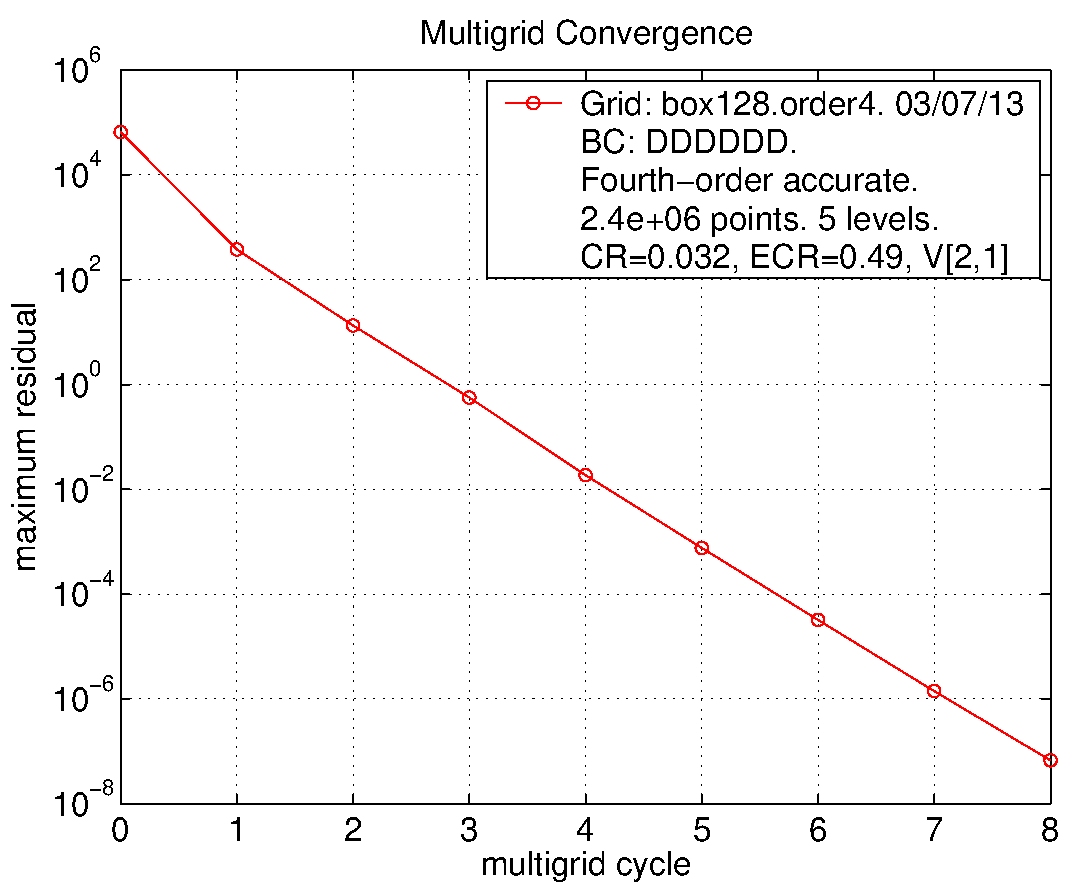
\includegraphics[width=.475\linewidth]{fig/residual_box128_order4}
  \end{center} 
\caption{Convergence history for a box, fourth-order.}
\label{fig:box}
\end{figure}




\begin{table}[hbt]
\begin{center}
\tablefontsize
\begin{tabular}{|c|c|c|c|c|} \hline 
 $i$   & $\vert\vert\mbox{res}\vert\vert_\infty$  &  CR     &  WU    & ECR  \\   \hline 
 $ 1$  & $ 3.7e+02$ & $0.022$ & $ 4.6$ & $0.44$ \\ 
 $ 2$  & $ 3.3e+01$ & $0.088$ & $ 3.6$ & $0.51$ \\ 
 $ 3$  & $ 1.8e+00$ & $0.057$ & $ 3.6$ & $0.45$ \\ 
 $ 4$  & $ 1.9e-01$ & $0.105$ & $ 3.6$ & $0.54$ \\ 
 $ 5$  & $ 1.2e-02$ & $0.060$ & $ 3.6$ & $0.46$ \\ 
 $ 6$  & $ 1.2e-03$ & $0.105$ & $ 3.6$ & $0.54$ \\ 
 $ 7$  & $ 9.9e-05$ & $0.081$ & $ 3.6$ & $0.50$ \\ 
 $ 8$  & $ 8.2e-06$ & $0.083$ & $ 3.6$ & $0.50$ \\ 
\hline 
\multicolumn{5}{|c|}{Grid: box64.order4. 03/07/13}  \\
\multicolumn{5}{|c|}{BC: DDDDDD.}  \\
\multicolumn{5}{|c|}{Fourth-order accurate.}  \\
\multicolumn{5}{|c|}{Trigonometric solution.}  \\
\multicolumn{5}{|c|}{V[1,1]: rb $\omega=1.20$}  \\
\multicolumn{5}{|c|}{3.29e+05 grid-points. 5 levels.}  \\
\multicolumn{5}{|c|}{Average CR=$0.069$, ECR=$0.49$.}  \\
\multicolumn{5}{|c|}{time/cycle = 2.32e-01 s.}  \\
\hline 
\end{tabular}
\begin{tabular}{|c|c|c|c|c|} \hline 
 $i$   & $\vert\vert\mbox{res}\vert\vert_\infty$  &  CR     &  WU    & ECR  \\   \hline 
 $ 1$  & $ 7.5e+01$ & $0.005$ & $ 7.0$ & $0.46$ \\ 
 $ 2$  & $ 3.1e+00$ & $0.042$ & $ 5.0$ & $0.53$ \\ 
 $ 3$  & $ 1.1e-01$ & $0.036$ & $ 5.0$ & $0.51$ \\ 
 $ 4$  & $ 3.8e-03$ & $0.034$ & $ 5.0$ & $0.50$ \\ 
 $ 5$  & $ 1.5e-04$ & $0.039$ & $ 5.0$ & $0.52$ \\ 
 $ 6$  & $ 6.0e-06$ & $0.041$ & $ 5.0$ & $0.52$ \\ 
 $ 7$  & $ 2.8e-07$ & $0.046$ & $ 5.0$ & $0.54$ \\ 
 $ 8$  & $ 1.3e-08$ & $0.047$ & $ 5.0$ & $0.54$ \\ 
\hline 
\multicolumn{5}{|c|}{Grid: box64.order4. 03/07/13}  \\
\multicolumn{5}{|c|}{BC: DDDDDD.}  \\
\multicolumn{5}{|c|}{Fourth-order accurate.}  \\
\multicolumn{5}{|c|}{Trigonometric solution.}  \\
\multicolumn{5}{|c|}{W[2,1]: rb $\omega=1.20$}  \\
\multicolumn{5}{|c|}{3.29e+05 grid-points. 5 levels.}  \\
\multicolumn{5}{|c|}{Average CR=$0.031$, ECR=$0.51$.}  \\
\multicolumn{5}{|c|}{time/cycle = 4.08e-01 s.}  \\
\hline 
\end{tabular}
\begin{tabular}{|c|c|c|c|c|} \hline 
 $i$   & $\vert\vert\mbox{res}\vert\vert_\infty$  &  CR     &  WU    & ECR  \\   \hline 
 $ 1$  & $ 3.9e+02$ & $0.024$ & $ 6.6$ & $0.57$ \\ 
 $ 2$  & $ 2.7e+01$ & $0.070$ & $ 4.6$ & $0.56$ \\ 
 $ 3$  & $ 2.4e+00$ & $0.089$ & $ 4.6$ & $0.59$ \\ 
 $ 4$  & $ 2.4e-01$ & $0.102$ & $ 4.6$ & $0.61$ \\ 
 $ 5$  & $ 2.5e-02$ & $0.101$ & $ 4.6$ & $0.61$ \\ 
 $ 6$  & $ 2.5e-03$ & $0.100$ & $ 4.6$ & $0.61$ \\ 
 $ 7$  & $ 2.5e-04$ & $0.101$ & $ 4.6$ & $0.61$ \\ 
 $ 8$  & $ 2.7e-05$ & $0.106$ & $ 4.6$ & $0.62$ \\ 
\hline 
\multicolumn{5}{|c|}{Grid: box64.order4. 03/07/13}  \\
\multicolumn{5}{|c|}{BC: DDDDDD.}  \\
\multicolumn{5}{|c|}{Fourth-order accurate. NO-OP-AVE}  \\
\multicolumn{5}{|c|}{Trigonometric solution.}  \\
\multicolumn{5}{|c|}{V[2,1]: rb $\omega=1.20$}  \\
\multicolumn{5}{|c|}{3.29e+05 grid-points. 5 levels.}  \\
\multicolumn{5}{|c|}{Average CR=$0.080$, ECR=$0.60$.}  \\
\multicolumn{5}{|c|}{time/cycle = 2.99e-01 s.}  \\
\hline 
\end{tabular}
\begin{tabular}{|c|c|c|c|c|} \hline 
 $i$   & $\vert\vert\mbox{res}\vert\vert_\infty$  &  CR     &  WU    & ECR  \\   \hline 
 $ 1$  & $ 9.3e+01$ & $0.006$ & $ 6.6$ & $0.46$ \\ 
 $ 2$  & $ 3.3e+00$ & $0.035$ & $ 4.6$ & $0.49$ \\ 
 $ 3$  & $ 1.3e-01$ & $0.041$ & $ 4.6$ & $0.50$ \\ 
 $ 4$  & $ 4.4e-03$ & $0.032$ & $ 4.6$ & $0.48$ \\ 
 $ 5$  & $ 1.7e-04$ & $0.038$ & $ 4.6$ & $0.49$ \\ 
 $ 6$  & $ 7.1e-06$ & $0.042$ & $ 4.6$ & $0.51$ \\ 
 $ 7$  & $ 3.1e-07$ & $0.043$ & $ 4.6$ & $0.51$ \\ 
 $ 8$  & $ 1.5e-08$ & $0.047$ & $ 4.6$ & $0.52$ \\ 
\hline 
\multicolumn{5}{|c|}{Grid: box64.order4. 03/07/13}  \\
\multicolumn{5}{|c|}{BC: DDDDDD.}  \\
\multicolumn{5}{|c|}{Fourth-order accurate.}  \\
\multicolumn{5}{|c|}{Trigonometric solution.}  \\
\multicolumn{5}{|c|}{V[2,1]: rb $\omega=1.20$}  \\
\multicolumn{5}{|c|}{3.29e+05 grid-points. 5 levels.}  \\
\multicolumn{5}{|c|}{Average CR=$0.031$, ECR=$0.49$.}  \\
\multicolumn{5}{|c|}{time/cycle = 3.05e-01 s.}  \\
\hline 
\end{tabular}
\begin{tabular}{|c|c|c|c|c|} \hline 
 $i$   & $\vert\vert\mbox{res}\vert\vert_\infty$  &  CR     &  WU    & ECR  \\   \hline 
 $ 1$  & $ 2.2e+01$ & $0.005$ & $ 6.7$ & $0.46$ \\ 
 $ 2$  & $ 7.4e-01$ & $0.033$ & $ 4.7$ & $0.48$ \\ 
 $ 3$  & $ 2.7e-02$ & $0.037$ & $ 4.7$ & $0.49$ \\ 
 $ 4$  & $ 7.7e-04$ & $0.028$ & $ 4.7$ & $0.46$ \\ 
 $ 5$  & $ 3.1e-05$ & $0.040$ & $ 4.7$ & $0.50$ \\ 
 $ 6$  & $ 1.3e-06$ & $0.041$ & $ 4.7$ & $0.50$ \\ 
 $ 7$  & $ 4.6e-08$ & $0.037$ & $ 4.7$ & $0.49$ \\ 
 $ 8$  & $ 1.8e-09$ & $0.039$ & $ 4.7$ & $0.50$ \\ 
\hline 
\multicolumn{5}{|c|}{Grid: box32.order4. 03/07/13}  \\
\multicolumn{5}{|c|}{BC: DDDDDD.}  \\
\multicolumn{5}{|c|}{Fourth-order accurate.}  \\
\multicolumn{5}{|c|}{Trigonometric solution.}  \\
\multicolumn{5}{|c|}{V[2,1]: rb $\omega=1.20$}  \\
\multicolumn{5}{|c|}{5.20e+04 grid-points. 4 levels.}  \\
\multicolumn{5}{|c|}{Average CR=$0.029$, ECR=$0.48$.}  \\
\multicolumn{5}{|c|}{time/cycle = 5.70e-02 s.}  \\
\hline 
\end{tabular}
\begin{tabular}{|c|c|c|c|c|} \hline 
 $i$   & $\vert\vert\mbox{res}\vert\vert_\infty$  &  CR     &  WU    & ECR  \\   \hline 
 $ 1$  & $ 3.8e+02$ & $0.006$ & $ 6.6$ & $0.46$ \\ 
 $ 2$  & $ 1.3e+01$ & $0.035$ & $ 4.6$ & $0.49$ \\ 
 $ 3$  & $ 5.6e-01$ & $0.042$ & $ 4.6$ & $0.50$ \\ 
 $ 4$  & $ 1.9e-02$ & $0.033$ & $ 4.6$ & $0.48$ \\ 
 $ 5$  & $ 7.6e-04$ & $0.041$ & $ 4.6$ & $0.50$ \\ 
 $ 6$  & $ 3.2e-05$ & $0.042$ & $ 4.6$ & $0.50$ \\ 
 $ 7$  & $ 1.4e-06$ & $0.044$ & $ 4.6$ & $0.51$ \\ 
 $ 8$  & $ 6.7e-08$ & $0.048$ & $ 4.6$ & $0.52$ \\ 
\hline 
\multicolumn{5}{|c|}{Grid: box128.order4. 03/07/13}  \\
\multicolumn{5}{|c|}{BC: DDDDDD.}  \\
\multicolumn{5}{|c|}{Fourth-order accurate.}  \\
\multicolumn{5}{|c|}{Trigonometric solution.}  \\
\multicolumn{5}{|c|}{V[2,1]: rb $\omega=1.20$}  \\
\multicolumn{5}{|c|}{2.35e+06 grid-points. 5 levels.}  \\
\multicolumn{5}{|c|}{Average CR=$0.032$, ECR=$0.49$.}  \\
\multicolumn{5}{|c|}{time/cycle = 2.32e+00 s.}  \\
\hline 
\end{tabular}
\begin{tabular}{|c|c|c|c|c|} \hline 
 $i$   & res      & rate    &  WU    & ECR  \\   \hline 
 $ 1$  & $ 6.0e+00$ & $0.020$ & $ 4.7$ & $0.43$ \\ 
 $ 2$  & $ 1.5e-01$ & $0.026$ & $ 4.7$ & $0.46$ \\ 
 $ 3$  & $ 4.8e-03$ & $0.031$ & $ 4.7$ & $0.47$ \\ 
 $ 4$  & $ 1.2e-04$ & $0.025$ & $ 4.7$ & $0.45$ \\ 
 $ 5$  & $ 2.1e-06$ & $0.017$ & $ 4.7$ & $0.42$ \\ 
 $ 6$  & $ 5.5e-08$ & $0.026$ & $ 4.7$ & $0.46$ \\ 
 $ 7$  & $ 1.3e-09$ & $0.025$ & $ 4.7$ & $0.45$ \\ 
\hline 
\multicolumn{5}{|c|}{Grid: box32.order4.}  \\
\multicolumn{5}{|c|}{Dirichlet boundary conditions.}  \\
\multicolumn{5}{|c|}{Fourth-order accurate.}  \\
\multicolumn{5}{|c|}{Trigonometric solution.}  \\
\multicolumn{5}{|c|}{Smoother rb[2,1] $\omega=1.20$}  \\
\multicolumn{5}{|c|}{5.20e+04 grid-points. 4 levels.}  \\
\multicolumn{5}{|c|}{Average CR=$0.024$, ECR=$0.45$.}  \\
\multicolumn{5}{|c|}{time/cycle = 2.29e-01 s.}  \\
\hline 
\end{tabular}
\begin{tabular}{|c|c|c|c|c|} \hline 
 $i$   & res      & rate    &  WU    & ECR  \\   \hline 
 $ 1$  & $ 1.7e+02$ & $0.044$ & $ 4.6$ & $0.51$ \\ 
 $ 2$  & $ 6.3e+00$ & $0.038$ & $ 4.6$ & $0.49$ \\ 
 $ 3$  & $ 2.5e-01$ & $0.040$ & $ 4.6$ & $0.50$ \\ 
 $ 4$  & $ 8.9e-03$ & $0.035$ & $ 4.6$ & $0.48$ \\ 
 $ 5$  & $ 3.3e-04$ & $0.037$ & $ 4.6$ & $0.49$ \\ 
 $ 6$  & $ 1.3e-05$ & $0.040$ & $ 4.6$ & $0.50$ \\ 
 $ 7$  & $ 5.8e-07$ & $0.043$ & $ 4.6$ & $0.51$ \\ 
\hline 
\multicolumn{5}{|c|}{Grid: box128.order4.}  \\
\multicolumn{5}{|c|}{Dirichlet boundary conditions.}  \\
\multicolumn{5}{|c|}{Fourth-order accurate.}  \\
\multicolumn{5}{|c|}{Trigonometric solution.}  \\
\multicolumn{5}{|c|}{Smoother rb[2,1] $\omega=1.15$}  \\
\multicolumn{5}{|c|}{2.35e+06 grid-points. 5 levels.}  \\
\multicolumn{5}{|c|}{Average CR=$0.040$, ECR=$0.50$.}  \\
\multicolumn{5}{|c|}{time/cycle = 3.48e+00 s.}  \\
\hline 
\end{tabular}
\begin{tabular}{|c|c|c|c|c|} \hline 
 $i$   & res      & rate    &  WU    & ECR  \\   \hline 
 $ 1$  & $ 1.3e+02$ & $0.025$ & $ 4.6$ & $0.45$ \\ 
 $ 2$  & $ 3.5e+00$ & $0.027$ & $ 4.6$ & $0.46$ \\ 
 $ 3$  & $ 1.7e-01$ & $0.048$ & $ 4.6$ & $0.52$ \\ 
 $ 4$  & $ 5.4e-03$ & $0.032$ & $ 4.6$ & $0.48$ \\ 
 $ 5$  & $ 1.9e-04$ & $0.035$ & $ 4.6$ & $0.48$ \\ 
 $ 6$  & $ 7.2e-06$ & $0.038$ & $ 4.6$ & $0.49$ \\ 
 $ 7$  & $ 2.7e-07$ & $0.037$ & $ 4.6$ & $0.49$ \\ 
\hline 
\multicolumn{5}{|c|}{Grid: box128.order4.}  \\
\multicolumn{5}{|c|}{Dirichlet boundary conditions.}  \\
\multicolumn{5}{|c|}{Fourth-order accurate.}  \\
\multicolumn{5}{|c|}{Trigonometric solution.}  \\
\multicolumn{5}{|c|}{Smoother rb[2,1] $\omega=1.20$}  \\
\multicolumn{5}{|c|}{2.35e+06 grid-points. 5 levels.}  \\
\multicolumn{5}{|c|}{Average CR=$0.034$, ECR=$0.48$.}  \\
\multicolumn{5}{|c|}{time/cycle = 3.47e+00 s.}  \\
\hline 
\end{tabular}
\end{center}
\caption{Multigrid convergence rates for a 3D box, fourth-order accuracy.}
\label{fig:smoothBox}
\end{table}

% ====================== OLD Box ================================

% \begin{table}[hbt]
% \begin{center}
% \begin{tabular}{|c|c|c|c|c|}                   \hline
%  $i$   & res(i)     & rate(i)    &  WU(i)     & ECR(i)  \\   \hline
%  $ 1$  & $ 1.8e+00$ & $ 9.2e-02$ & $ 4.8$ & $0.61$ \\ 
%  $ 2$  & $ 1.7e-01$ & $ 9.1e-02$ & $ 4.8$ & $0.60$ \\ 
%  $ 3$  & $ 1.5e-02$ & $ 9.1e-02$ & $ 4.8$ & $0.60$ \\ 
%  $ 4$  & $ 1.5e-03$ & $ 1.0e-01$ & $ 4.8$ & $0.62$ \\ 
%  \hline
%  \multicolumn{5}{c}{Red-Black, box8mg}         \\
%  \multicolumn{5}{c}{2 levels, $n_s=3$, Dirichlet}         \\
% \end{tabular}
% \qquad\qquad
% \begin{tabular}{|c|c|c|c|c|}                   \hline
%  $i$   & res(i)     & rate(i)    &  WU(i)     & ECR(i)  \\   \hline
%  $ 1$  & $ 8.8e+00$ & $0.080$ & $ 4.8$ & $0.59$ \\ 
%  $ 2$  & $ 7.7e-01$ & $0.087$ & $ 4.8$ & $0.60$ \\ 
%  $ 3$  & $ 6.7e-02$ & $0.088$ & $ 4.8$ & $0.60$ \\ 
%  $ 4$  & $ 6.0e-03$ & $0.088$ & $ 4.8$ & $0.60$ \\ 
%  $ 5$  & $ 5.3e-04$ & $0.089$ & $ 4.8$ & $0.60$ \\ 
%  $ 6$  & $ 4.7e-05$ & $0.089$ & $ 4.8$ & $0.60$ \\ 
%  $ 7$  & $ 4.3e-06$ & $0.090$ & $ 4.8$ & $0.60$ \\ 
%  $ 8$  & $ 3.9e-07$ & $0.091$ & $ 4.8$ & $0.60$ \\ 
%  $ 9$  & $ 3.5e-08$ & $0.091$ & $ 4.8$ & $0.61$ \\ 
%  $10$  & $ 3.2e-09$ & $0.092$ & $ 4.8$ & $0.61$ \\ 
%  $11$  & $ 3.0e-10$ & $0.092$ & $ 4.8$ & $0.61$ \\ 
%  \hline
%  \multicolumn{5}{c}{Red-Black, box16bmg}         \\
%  \multicolumn{5}{c}{4 levels, $n_s=3$, Dirichlet}         \\
% \end{tabular}
% \qquad\qquad
% \begin{tabular}{|c|c|c|c|c|}                   \hline
%  $i$   & res(i)     & rate(i)    &  WU(i)     & ECR(i)  \\   \hline
%  $ 1$  & $ 1.5e+02$ & $0.080$ & $ 4.7$ & $0.58$ \\ 
%  $ 2$  & $ 1.3e+01$ & $0.087$ & $ 4.7$ & $0.59$ \\ 
%  $ 3$  & $ 1.2e+00$ & $0.087$ & $ 4.7$ & $0.59$ \\ 
%  $ 4$  & $ 1.0e-01$ & $0.088$ & $ 4.7$ & $0.60$ \\ 
%  $ 5$  & $ 9.1e-03$ & $0.088$ & $ 4.7$ & $0.60$ \\ 
%  $ 6$  & $ 8.1e-04$ & $0.089$ & $ 4.7$ & $0.60$ \\ 
%  $ 7$  & $ 7.2e-05$ & $0.089$ & $ 4.7$ & $0.60$ \\ 
%  $ 8$  & $ 6.5e-06$ & $0.090$ & $ 4.7$ & $0.60$ \\ 
%  $ 9$  & $ 5.8e-07$ & $0.090$ & $ 4.7$ & $0.60$ \\ 
%  $10$  & $ 5.3e-08$ & $0.091$ & $ 4.7$ & $0.60$ \\ 
%  \hline
%  \multicolumn{5}{c}{Red-Black, box64bmg}         \\
%  \multicolumn{5}{c}{5 levels, $n_s=3$, Dirichlet}         \\
% \end{tabular}
% \end{center}
% \caption{Multigrid convergence rates for a 3D box.}
% \label{fig:smoothBox}
% \end{table}
% 
% \begin{table}[hbt]
% \begin{center}
% \begin{tabular}{|c|c|c|c|c|} \hline 
%  $i$   & res      & rate    &  WU    & ECR  \\   \hline 
%  $ 1$  & $ 1.3e+01$ & $0.061$ & $ 4.6$ & $0.55$ \\ 
%  $ 2$  & $ 9.2e-01$ & $0.068$ & $ 4.6$ & $0.56$ \\ 
%  $ 3$  & $ 6.6e-02$ & $0.072$ & $ 4.6$ & $0.57$ \\ 
%  $ 4$  & $ 4.6e-03$ & $0.071$ & $ 4.6$ & $0.57$ \\ 
%  $ 5$  & $ 3.3e-04$ & $0.072$ & $ 4.6$ & $0.57$ \\ 
%  $ 6$  & $ 2.4e-05$ & $0.072$ & $ 4.6$ & $0.57$ \\ 
%  $ 7$  & $ 1.7e-06$ & $0.073$ & $ 4.6$ & $0.57$ \\ 
%  $ 8$  & $ 1.3e-07$ & $0.073$ & $ 4.6$ & $0.57$ \\ 
% \hline 
% \multicolumn{5}{|c|}{Grid: box32.}  \\
% \multicolumn{5}{|c|}{Dirichlet boundary conditions.}  \\
% \multicolumn{5}{|c|}{Trigonometric solution.}  \\
% \multicolumn{5}{|c|}{Smoother rb[2,1]}  \\
% \multicolumn{5}{|c|}{5.07e+04 grid-points. 5 levels.}  \\
% \multicolumn{5}{|c|}{Average CR=$0.070$, ECR=$0.56$.}  \\
% \hline 
% \end{tabular}
% \qquad % --------------------------------------------------------------------
% \begin{tabular}{|c|c|c|c|c|} \hline 
%  $i$   & res      & rate    &  WU    & ECR  \\   \hline 
%  $ 1$  & $ 3.2e+02$ & $0.080$ & $ 4.6$ & $0.58$ \\ 
%  $ 2$  & $ 2.5e+01$ & $0.079$ & $ 4.6$ & $0.58$ \\ 
%  $ 3$  & $ 2.0e+00$ & $0.079$ & $ 4.6$ & $0.58$ \\ 
%  $ 4$  & $ 1.6e-01$ & $0.081$ & $ 4.6$ & $0.58$ \\ 
%  $ 5$  & $ 1.3e-02$ & $0.082$ & $ 4.6$ & $0.58$ \\ 
%  $ 6$  & $ 1.1e-03$ & $0.082$ & $ 4.6$ & $0.58$ \\ 
%  $ 7$  & $ 9.1e-05$ & $0.083$ & $ 4.6$ & $0.58$ \\ 
%  $ 8$  & $ 7.5e-06$ & $0.083$ & $ 4.6$ & $0.58$ \\ 
% \hline 
% \multicolumn{5}{|c|}{Grid: box128.}  \\
% \multicolumn{5}{|c|}{Dirichlet boundary conditions.}  \\
% \multicolumn{5}{|c|}{Trigonometric solution.}  \\
% \multicolumn{5}{|c|}{Smoother rb[2,1]}  \\
% \multicolumn{5}{|c|}{2.35e+06 grid-points. 5 levels.}  \\
% \multicolumn{5}{|c|}{Average CR=$0.081$, ECR=$0.58$.}  \\
% \hline 
% \end{tabular}
% %\qquad % --------------------------------------------------------------------
% \vskip\baselineskip
% \begin{tabular}{|c|c|c|c|c|} \hline 
%  $i$   & res      & rate    &  WU    & ECR  \\   \hline 
%  $ 1$  & $ 2.3e-02$ & $0.029$ & $ 4.6$ & $0.47$ \\ 
%  $ 2$  & $ 1.7e-03$ & $0.071$ & $ 4.6$ & $0.56$ \\ 
%  $ 3$  & $ 1.2e-04$ & $0.074$ & $ 4.6$ & $0.57$ \\ 
%  $ 4$  & $ 9.3e-06$ & $0.076$ & $ 4.6$ & $0.57$ \\ 
%  $ 5$  & $ 7.2e-07$ & $0.078$ & $ 4.6$ & $0.58$ \\ 
%  $ 6$  & $ 5.7e-08$ & $0.079$ & $ 4.6$ & $0.58$ \\ 
%  $ 7$  & $ 4.6e-09$ & $0.080$ & $ 4.6$ & $0.58$ \\ 
% \hline 
% \multicolumn{5}{|c|}{Grid: box256.}  \\
% \multicolumn{5}{|c|}{Dirichlet boundary conditions.}  \\
% \multicolumn{5}{|c|}{Constant forcing.}  \\
% \multicolumn{5}{|c|}{Smoother rb[2,1]}  \\
% \multicolumn{5}{|c|}{1.78e+07 grid-points. 5 levels.}  \\
% \multicolumn{5}{|c|}{Average CR=$0.067$, ECR=$0.56$.}  \\
% \hline 
% \end{tabular}
% \qquad % --------------------------------------------------------------------
% \begin{tabular}{|c|c|c|c|c|} \hline 
%  $i$   & res      & rate    &  WU    & ECR  \\   \hline 
%  $ 1$  & $ 7.9e+01$ & $0.028$ & $ 4.6$ & $0.46$ \\ 
%  $ 2$  & $ 1.5e+00$ & $0.019$ & $ 4.6$ & $0.42$ \\ 
%  $ 3$  & $ 2.5e-02$ & $0.017$ & $ 4.6$ & $0.41$ \\ 
%  $ 4$  & $ 5.1e-04$ & $0.021$ & $ 4.6$ & $0.43$ \\ 
%  $ 5$  & $ 9.4e-06$ & $0.018$ & $ 4.6$ & $0.42$ \\ 
%  $ 6$  & $ 1.6e-07$ & $0.017$ & $ 4.6$ & $0.41$ \\ 
%  $ 7$  & $ 3.0e-09$ & $0.019$ & $ 4.6$ & $0.43$ \\ 
%  $ 8$  & $ 7.6e-11$ & $0.025$ & $ 4.6$ & $0.45$ \\ 
% \hline 
% \multicolumn{5}{|c|}{Grid: box128.}  \\
% \multicolumn{5}{|c|}{Dirichlet boundary conditions.}  \\
% \multicolumn{5}{|c|}{Trigonometric solution.}  \\
% \multicolumn{5}{|c|}{Smoother rb[2,1], omega=1.15}  \\
% \multicolumn{5}{|c|}{2.35e+06 grid-points. 5 levels.}  \\
% \multicolumn{5}{|c|}{Average CR=$0.020$, ECR=$0.43$.}  \\
% \hline 
% \end{tabular}
% \end{center}
% \caption{Multigrid convergence rates for a box, second-order accuracy.}
%  \label{tab:square4} 
% \end{table}
% 

\clearpage
% ===================================================================================================
\subsection{Cylinder}

\begin{figure}[hbt]
\begin{center}
  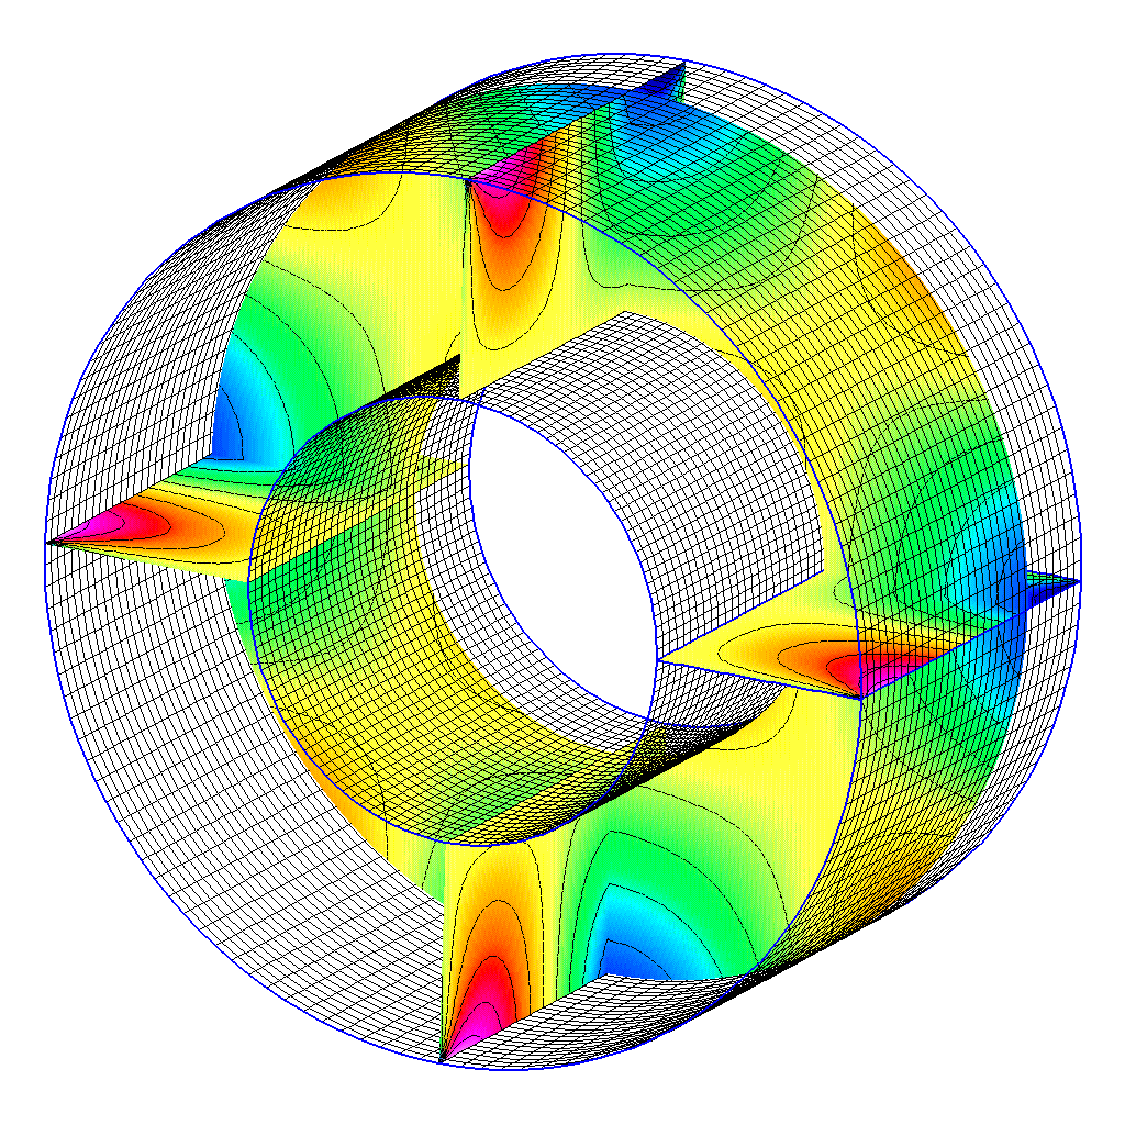
\includegraphics[width=.75\linewidth]{fig/cylinder3_u}
  \end{center} 
\caption{Cylinder grid and solution, (cylinder3)}
\label{fig:cylinder3}
\end{figure}



\begin{table}[hbt]
\begin{center}
\begin{tabular}{|c|c|c|c|c|} \hline 
 $i$   & $\vert\vert\mbox{res}\vert\vert_\infty$  &  CR     &  WU    & ECR  \\   \hline 
 $ 1$  & $ 2.1e+01$ & $0.098$ & $ 5.0$ & $0.63$ \\ 
 $ 2$  & $ 2.0e+00$ & $0.096$ & $ 5.0$ & $0.62$ \\ 
 $ 3$  & $ 2.3e-01$ & $0.112$ & $ 5.0$ & $0.64$ \\ 
 $ 4$  & $ 2.3e-02$ & $0.100$ & $ 5.0$ & $0.63$ \\ 
 $ 5$  & $ 2.7e-03$ & $0.117$ & $ 5.0$ & $0.65$ \\ 
 $ 6$  & $ 2.9e-04$ & $0.108$ & $ 5.0$ & $0.64$ \\ 
 $ 7$  & $ 3.3e-05$ & $0.114$ & $ 5.0$ & $0.65$ \\ 
 $ 8$  & $ 3.6e-06$ & $0.109$ & $ 5.0$ & $0.64$ \\ 
 $ 9$  & $ 4.1e-07$ & $0.113$ & $ 5.0$ & $0.64$ \\ 
\hline 
\multicolumn{5}{|c|}{Grid: cylinder3.}  \\
\multicolumn{5}{|c|}{BC: PPPPDD.}  \\
\multicolumn{5}{|c|}{Second-order accurate.}  \\
\multicolumn{5}{|c|}{Trigonometric solution.}  \\
\multicolumn{5}{|c|}{W[2,1]: rb $\omega=1.43$ (VAR)}  \\
\multicolumn{5}{|c|}{2.21e+05 grid-points. 4 levels.}  \\
\multicolumn{5}{|c|}{Average CR=$0.107$, ECR=$0.64$.}  \\
\multicolumn{5}{|c|}{time/cycle = 5.66e-01 s.}  \\
\hline 
\end{tabular}
\qquad
\begin{tabular}{|c|c|c|c|c|} \hline 
 $i$   & $\vert\vert\mbox{res}\vert\vert_\infty$  &  CR     &  WU    & ECR  \\   \hline 
 $ 1$  & $ 2.6e+01$ & $0.113$ & $ 4.6$ & $0.62$ \\ 
 $ 2$  & $ 2.4e+00$ & $0.092$ & $ 4.6$ & $0.60$ \\ 
 $ 3$  & $ 3.1e-01$ & $0.127$ & $ 4.6$ & $0.64$ \\ 
 $ 4$  & $ 3.1e-02$ & $0.103$ & $ 4.6$ & $0.61$ \\ 
 $ 5$  & $ 3.7e-03$ & $0.118$ & $ 4.6$ & $0.63$ \\ 
 $ 6$  & $ 5.1e-04$ & $0.136$ & $ 4.6$ & $0.65$ \\ 
 $ 7$  & $ 9.4e-05$ & $0.185$ & $ 4.6$ & $0.70$ \\ 
 $ 8$  & $ 2.0e-05$ & $0.214$ & $ 4.6$ & $0.72$ \\ 
 $ 9$  & $ 4.2e-06$ & $0.211$ & $ 4.6$ & $0.72$ \\ 
\hline 
\multicolumn{5}{|c|}{Grid: cylinder3.}  \\
\multicolumn{5}{|c|}{BC: PPPPDD.}  \\
\multicolumn{5}{|c|}{Second-order accurate.}  \\
\multicolumn{5}{|c|}{Trigonometric solution.}  \\
\multicolumn{5}{|c|}{V[2,1]: rb $\omega=1.43$ (VAR)}  \\
\multicolumn{5}{|c|}{2.21e+05 grid-points. 4 levels.}  \\
\multicolumn{5}{|c|}{Average CR=$0.138$, ECR=$0.65$.}  \\
\multicolumn{5}{|c|}{time/cycle = 4.94e-01 s.}  \\
\hline 
\end{tabular}
\vskip\baselineskip
\begin{tabular}{|c|c|c|c|c|} \hline 
 $i$   & $\vert\vert\mbox{res}\vert\vert_\infty$  &  CR     &  WU    & ECR  \\   \hline 
 $ 1$  & $ 1.7e+01$ & $0.094$ & $ 5.0$ & $0.62$ \\ 
 $ 2$  & $ 1.5e+00$ & $0.085$ & $ 5.0$ & $0.61$ \\ 
 $ 3$  & $ 1.5e-01$ & $0.103$ & $ 5.0$ & $0.63$ \\ 
 $ 4$  & $ 1.5e-02$ & $0.096$ & $ 5.0$ & $0.62$ \\ 
 $ 5$  & $ 1.6e-03$ & $0.108$ & $ 5.0$ & $0.64$ \\ 
 $ 6$  & $ 1.6e-04$ & $0.102$ & $ 5.0$ & $0.63$ \\ 
 $ 7$  & $ 1.7e-05$ & $0.108$ & $ 5.0$ & $0.64$ \\ 
 $ 8$  & $ 1.9e-06$ & $0.107$ & $ 5.0$ & $0.64$ \\ 
 $ 9$  & $ 2.4e-07$ & $0.126$ & $ 5.0$ & $0.66$ \\ 
\hline 
\multicolumn{5}{|c|}{Grid: cylinder3.}  \\
\multicolumn{5}{|c|}{BC: PPPPDD.}  \\
\multicolumn{5}{|c|}{Second-order accurate.}  \\
\multicolumn{5}{|c|}{Trigonometric solution.}  \\
\multicolumn{5}{|c|}{W[2,1]: rb $\omega=1.40$ (CONST)}  \\
\multicolumn{5}{|c|}{2.21e+05 grid-points. 4 levels.}  \\
\multicolumn{5}{|c|}{Average CR=$0.103$, ECR=$0.63$.}  \\
\multicolumn{5}{|c|}{time/cycle = 5.05e-01 s.}  \\
\hline 
\end{tabular}
\qquad
\begin{tabular}{|c|c|c|c|c|} \hline 
 $i$   & $\vert\vert\mbox{res}\vert\vert_\infty$  &  CR     &  WU    & ECR  \\   \hline 
 $ 1$  & $ 2.8e+01$ & $0.251$ & $ 5.0$ & $0.76$ \\ 
 $ 2$  & $ 8.4e+00$ & $0.303$ & $ 5.0$ & $0.79$ \\ 
 $ 3$  & $ 2.7e+00$ & $0.321$ & $ 5.0$ & $0.80$ \\ 
 $ 4$  & $ 9.4e-01$ & $0.349$ & $ 5.0$ & $0.81$ \\ 
 $ 5$  & $ 3.3e-01$ & $0.357$ & $ 5.0$ & $0.81$ \\ 
 $ 6$  & $ 1.2e-01$ & $0.363$ & $ 5.0$ & $0.82$ \\ 
 $ 7$  & $ 4.5e-02$ & $0.373$ & $ 5.0$ & $0.82$ \\ 
 $ 8$  & $ 1.7e-02$ & $0.382$ & $ 5.0$ & $0.82$ \\ 
 $ 9$  & $ 6.7e-03$ & $0.385$ & $ 5.0$ & $0.82$ \\ 
\hline 
\multicolumn{5}{|c|}{Grid: cylinder3.}  \\
\multicolumn{5}{|c|}{BC: PPPPDD.}  \\
\multicolumn{5}{|c|}{Second-order accurate.}  \\
\multicolumn{5}{|c|}{Trigonometric solution.}  \\
\multicolumn{5}{|c|}{W[2,1]: rb $\omega=1.00$ (CONST)}  \\
\multicolumn{5}{|c|}{2.21e+05 grid-points. 4 levels.}  \\
\multicolumn{5}{|c|}{Average CR=$0.340$, ECR=$0.80$.}  \\
\multicolumn{5}{|c|}{time/cycle = 5.08e-01 s.}  \\
\hline 
\end{tabular}
\end{center}
\caption{Multigrid convergence rates for a cylinder.}
\label{fig:cylinder}
\end{table}


\begin{table}[hbt]
\begin{center}
\begin{tabular}{|c|c|c|c|c|} \hline 
 $i$   & $\vert\vert\mbox{res}\vert\vert_\infty$  &  CR     &  WU    & ECR  \\   \hline 
 $ 1$  & $ 2.3e+01$ & $0.318$ & $ 5.4$ & $0.81$ \\ 
 $ 2$  & $ 3.6e-01$ & $0.015$ & $ 5.4$ & $0.46$ \\ 
 $ 3$  & $ 1.3e-01$ & $0.364$ & $ 5.3$ & $0.83$ \\ 
 $ 4$  & $ 3.5e-02$ & $0.271$ & $ 5.3$ & $0.78$ \\ 
 $ 5$  & $ 1.0e-03$ & $0.029$ & $ 5.3$ & $0.51$ \\ 
 $ 6$  & $ 4.0e-04$ & $0.391$ & $ 5.3$ & $0.84$ \\ 
 $ 7$  & $ 1.2e-04$ & $0.296$ & $ 5.3$ & $0.79$ \\ 
 $ 8$  & $ 5.1e-06$ & $0.043$ & $ 5.3$ & $0.55$ \\ 
 $ 9$  & $ 2.4e-06$ & $0.472$ & $ 5.3$ & $0.87$ \\ 
\hline 
\multicolumn{5}{|c|}{Grid: cylinder3.}  \\
\multicolumn{5}{|c|}{BC: PPPPDD.}  \\
\multicolumn{5}{|c|}{Second-order accurate.}  \\
\multicolumn{5}{|c|}{Trigonometric solution.}  \\
\multicolumn{5}{|c|}{W[2,1]: alz $\omega=1.00$}  \\
\multicolumn{5}{|c|}{2.21e+05 grid-points. 4 levels.}  \\
\multicolumn{5}{|c|}{Average CR=$0.147$, ECR=$0.70$.}  \\
\multicolumn{5}{|c|}{time/cycle = 5.94e-01 s.}  \\
\hline 
\end{tabular}
\qquad
\begin{tabular}{|c|c|c|c|c|} \hline 
 $i$   & $\vert\vert\mbox{res}\vert\vert_\infty$  &  CR     &  WU    & ECR  \\   \hline 
 $ 1$  & $ 4.6e+00$ & $0.050$ & $ 5.4$ & $0.57$ \\ 
 $ 2$  & $ 1.2e-01$ & $0.027$ & $ 5.4$ & $0.51$ \\ 
 $ 3$  & $ 1.2e-02$ & $0.098$ & $ 5.3$ & $0.64$ \\ 
 $ 4$  & $ 1.1e-03$ & $0.092$ & $ 5.3$ & $0.64$ \\ 
 $ 5$  & $ 3.4e-05$ & $0.031$ & $ 5.3$ & $0.52$ \\ 
 $ 6$  & $ 3.2e-06$ & $0.094$ & $ 5.3$ & $0.64$ \\ 
 $ 7$  & $ 4.1e-07$ & $0.128$ & $ 5.3$ & $0.68$ \\ 
 $ 8$  & $ 1.3e-08$ & $0.031$ & $ 5.3$ & $0.52$ \\ 
 $ 9$  & $ 2.1e-09$ & $0.171$ & $ 5.3$ & $0.72$ \\ 
\hline 
\multicolumn{5}{|c|}{Grid: cylinder3.}  \\
\multicolumn{5}{|c|}{BC: PPPPDD.}  \\
\multicolumn{5}{|c|}{Second-order accurate.}  \\
\multicolumn{5}{|c|}{Trigonometric solution.}  \\
\multicolumn{5}{|c|}{W[2,1]: alz $\omega=1.30$}  \\
\multicolumn{5}{|c|}{2.21e+05 grid-points. 4 levels.}  \\
\multicolumn{5}{|c|}{Average CR=$0.066$, ECR=$0.60$.}  \\
\multicolumn{5}{|c|}{time/cycle = 5.88e-01 s.}  \\
\hline 
\end{tabular}
\vskip\baselineskip
\begin{tabular}{|c|c|c|c|c|} \hline 
 $i$   & $\vert\vert\mbox{res}\vert\vert_\infty$  &  CR     &  WU    & ECR  \\   \hline 
 $ 1$  & $ 4.7e+00$ & $0.051$ & $ 5.8$ & $0.60$ \\ 
 $ 2$  & $ 1.2e-01$ & $0.026$ & $ 5.8$ & $0.53$ \\ 
 $ 3$  & $ 1.2e-02$ & $0.098$ & $ 5.7$ & $0.66$ \\ 
 $ 4$  & $ 1.1e-03$ & $0.092$ & $ 5.7$ & $0.66$ \\ 
 $ 5$  & $ 3.5e-05$ & $0.031$ & $ 5.7$ & $0.54$ \\ 
 $ 6$  & $ 3.2e-06$ & $0.091$ & $ 5.7$ & $0.66$ \\ 
 $ 7$  & $ 4.1e-07$ & $0.129$ & $ 5.7$ & $0.70$ \\ 
 $ 8$  & $ 1.2e-08$ & $0.028$ & $ 5.7$ & $0.53$ \\ 
 $ 9$  & $ 1.4e-09$ & $0.118$ & $ 5.7$ & $0.69$ \\ 
\hline 
\multicolumn{5}{|c|}{Grid: cylinder3.}  \\
\multicolumn{5}{|c|}{BC: PPPPDD.}  \\
\multicolumn{5}{|c|}{Second-order accurate.}  \\
\multicolumn{5}{|c|}{Trigonometric solution.}  \\
\multicolumn{5}{|c|}{C3[2,1]: alz $\omega=1.30$}  \\
\multicolumn{5}{|c|}{2.21e+05 grid-points. 4 levels.}  \\
\multicolumn{5}{|c|}{Average CR=$0.063$, ECR=$0.61$.}  \\
\multicolumn{5}{|c|}{time/cycle = 6.94e-01 s.}  \\
\hline 
\end{tabular}
\qquad
\end{center}
\caption{Multigrid convergence rates for a cylinder - over-relaxation for SPLIT line-zebra.}
\label{fig:cylinder}
\end{table}

\begin{table}[hbt]
\begin{center}
\begin{tabular}{|c|c|c|c|c|} \hline 
 $i$   & $\vert\vert\mbox{res}\vert\vert_\infty$  &  CR     &  WU    & ECR  \\   \hline 
 $ 1$  & $ 1.3e-02$ & $0.008$ & $12.2$ & $0.68$ \\ 
 $ 2$  & $ 2.8e-04$ & $0.022$ & $12.2$ & $0.73$ \\ 
 $ 3$  & $ 6.7e-06$ & $0.024$ & $12.2$ & $0.74$ \\ 
 $ 4$  & $ 1.7e-07$ & $0.025$ & $12.2$ & $0.74$ \\ 
 $ 5$  & $ 4.3e-09$ & $0.026$ & $12.2$ & $0.74$ \\ 
 $ 6$  & $ 1.1e-10$ & $0.026$ & $12.2$ & $0.74$ \\ 
\hline 
\multicolumn{5}{|c|}{Grid: cylinder3.}  \\
\multicolumn{5}{|c|}{BC: PPPPDD.}  \\
\multicolumn{5}{|c|}{Second-order accurate.}  \\
\multicolumn{5}{|c|}{Trigonometric solution.}  \\
\multicolumn{5}{|c|}{W[2,1]: alz $\omega=1.00$}  \\
\multicolumn{5}{|c|}{2.21e+05 grid-points. 4 levels.}  \\
\multicolumn{5}{|c|}{Average CR=$0.020$, ECR=$0.73$.}  \\
\multicolumn{5}{|c|}{time/cycle = 1.38e+00 s.}  \\
\hline 
\end{tabular}
\qquad
\begin{tabular}{|c|c|c|c|c|} \hline 
 $i$   & $\vert\vert\mbox{res}\vert\vert_\infty$  &  CR     &  WU    & ECR  \\   \hline 
 $ 1$  & $ 2.8e-02$ & $0.009$ & $12.2$ & $0.68$ \\ 
 $ 2$  & $ 2.6e-04$ & $0.009$ & $12.2$ & $0.68$ \\ 
 $ 3$  & $ 2.4e-06$ & $0.009$ & $12.2$ & $0.68$ \\ 
 $ 4$  & $ 2.4e-08$ & $0.010$ & $12.2$ & $0.69$ \\ 
 $ 5$  & $ 2.4e-10$ & $0.010$ & $12.2$ & $0.69$ \\ 
\hline 
\multicolumn{5}{|c|}{Grid: cylinder3.}  \\
\multicolumn{5}{|c|}{BC: PPPPDD.}  \\
\multicolumn{5}{|c|}{Second-order accurate.}  \\
\multicolumn{5}{|c|}{Trigonometric solution.}  \\
\multicolumn{5}{|c|}{W[2,1]: alz $\omega=1.15$}  \\
\multicolumn{5}{|c|}{2.21e+05 grid-points. 4 levels.}  \\
\multicolumn{5}{|c|}{Average CR=$0.009$, ECR=$0.68$.}  \\
\multicolumn{5}{|c|}{time/cycle = 1.40e+00 s.}  \\
\hline 
\end{tabular}
\vskip\baselineskip
\begin{tabular}{|c|c|c|c|c|} \hline 
 $i$   & $\vert\vert\mbox{res}\vert\vert_\infty$  &  CR     &  WU    & ECR  \\   \hline 
 $ 1$  & $ 3.6e-02$ & $0.010$ & $11.7$ & $0.68$ \\ 
 $ 2$  & $ 3.8e-04$ & $0.011$ & $11.7$ & $0.68$ \\ 
 $ 3$  & $ 3.9e-06$ & $0.010$ & $11.7$ & $0.68$ \\ 
 $ 4$  & $ 4.3e-08$ & $0.011$ & $11.7$ & $0.68$ \\ 
 $ 5$  & $ 4.4e-10$ & $0.010$ & $11.7$ & $0.68$ \\ 
 $ 6$  & $ 7.1e-12$ & $0.016$ & $11.7$ & $0.70$ \\ 
\hline 
\multicolumn{5}{|c|}{Grid: cylinder3.}  \\
\multicolumn{5}{|c|}{BC: PPPPDD.}  \\
\multicolumn{5}{|c|}{Second-order accurate.}  \\
\multicolumn{5}{|c|}{Trigonometric solution.}  \\
\multicolumn{5}{|c|}{V[2,1]: alz $\omega=1.15$}  \\
\multicolumn{5}{|c|}{2.21e+05 grid-points. 4 levels.}  \\
\multicolumn{5}{|c|}{Average CR=$0.011$, ECR=$0.68$.}  \\
\multicolumn{5}{|c|}{time/cycle = 1.18e+00 s.}  \\
\hline 
\end{tabular}
\qquad
\begin{tabular}{|c|c|c|c|c|} \hline 
 $i$   & $\vert\vert\mbox{res}\vert\vert_\infty$  &  CR     &  WU    & ECR  \\   \hline 
 $ 1$  & $ 1.2e-01$ & $0.009$ & $12.2$ & $0.68$ \\ 
 $ 2$  & $ 1.1e-03$ & $0.010$ & $12.2$ & $0.68$ \\ 
 $ 3$  & $ 1.0e-05$ & $0.009$ & $12.2$ & $0.68$ \\ 
 $ 4$  & $ 1.0e-07$ & $0.010$ & $12.2$ & $0.69$ \\ 
 $ 5$  & $ 2.2e-09$ & $0.021$ & $12.2$ & $0.73$ \\ 
\hline 
\multicolumn{5}{|c|}{Grid: cylinder4.}  \\
\multicolumn{5}{|c|}{BC: PPPPDD.}  \\
\multicolumn{5}{|c|}{Second-order accurate.}  \\
\multicolumn{5}{|c|}{Trigonometric solution.}  \\
\multicolumn{5}{|c|}{W[2,1]: alz $\omega=1.15$}  \\
\multicolumn{5}{|c|}{1.53e+06 grid-points. 5 levels.}  \\
\multicolumn{5}{|c|}{Average CR=$0.011$, ECR=$0.69$.}  \\
\multicolumn{5}{|c|}{time/cycle = 1.05e+01 s.}  \\
\hline 
\end{tabular}
\qquad
\end{center}
\caption{Multigrid convergence rates for a cylinder - over-relaxation for TRUE line-zebra.}
\label{fig:cylinder}
\end{table}

% ===================================================================================
\clearpage
\subsection{Ortho-sphere}

\begin{figure}[hbt]
\begin{center}
  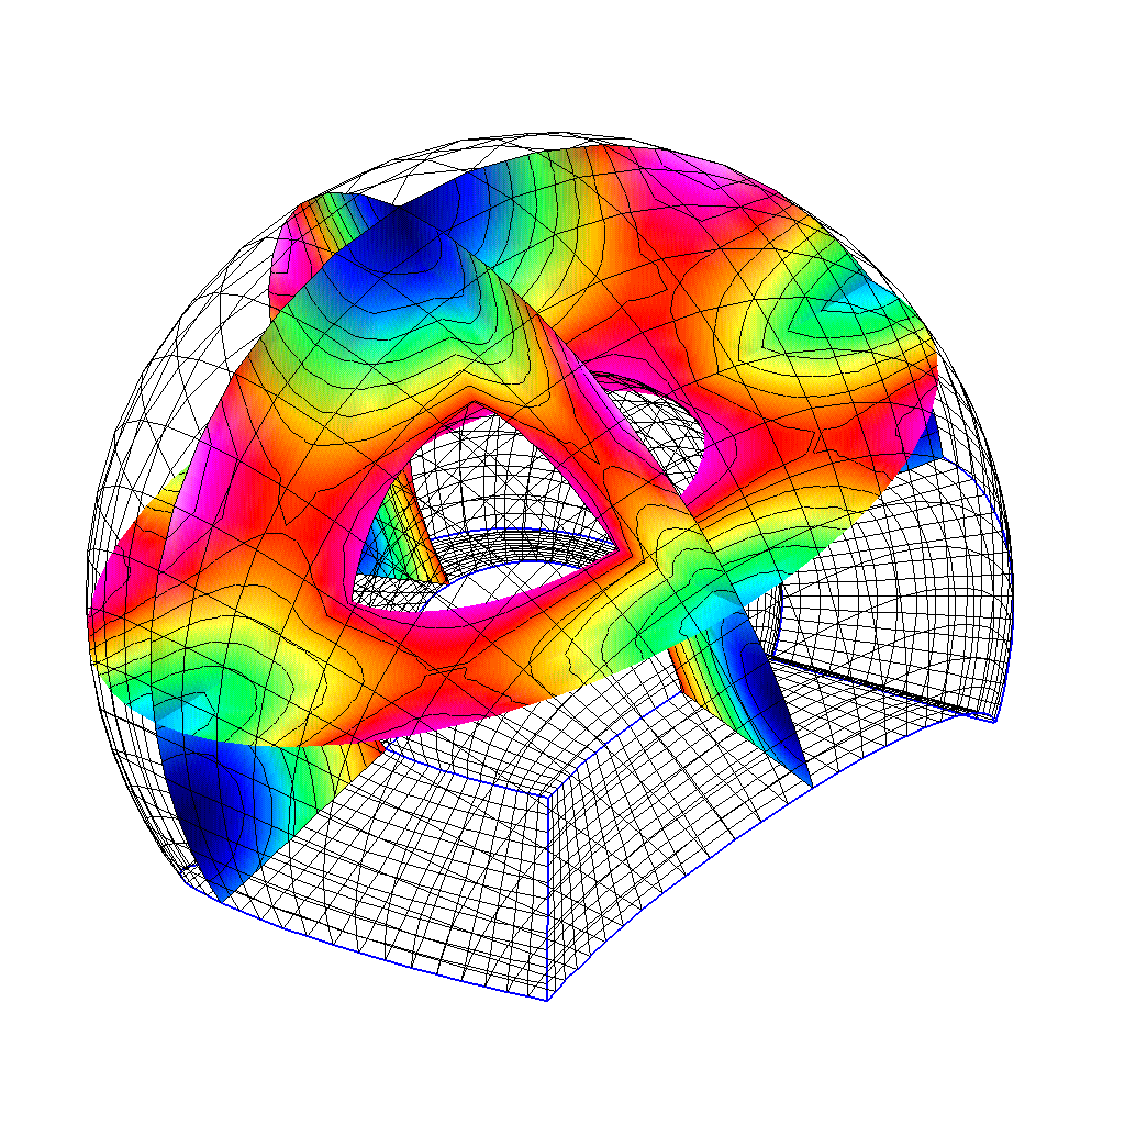
\includegraphics[width=.75\linewidth]{fig/orthoSphere2_u}
  \end{center} 
\caption{Orthographic grid on a part of the sphere, (orthoSphere2)}
\label{fig:orthoSphere2}
\end{figure}


\begin{table}[hbt]
\begin{center}
{\tablefontsize
\begin{tabular}{|c|c|c|c|c|} \hline 
 $i$   & $\vert\vert\mbox{res}\vert\vert_\infty$  &  CR     &  WU    & ECR  \\   \hline 
 $ 1$  & $ 3.3e-02$ & $0.012$ & $11.8$ & $0.69$ \\ 
 $ 2$  & $ 4.1e-04$ & $0.013$ & $11.8$ & $0.69$ \\ 
 $ 3$  & $ 6.1e-06$ & $0.015$ & $11.8$ & $0.70$ \\ 
 $ 4$  & $ 9.1e-08$ & $0.015$ & $11.8$ & $0.70$ \\ 
 $ 5$  & $ 1.4e-09$ & $0.015$ & $11.8$ & $0.70$ \\ 
 $ 6$  & $ 2.0e-11$ & $0.015$ & $11.8$ & $0.70$ \\ 
\hline 
\multicolumn{5}{|c|}{Grid: orthoSphere3.}  \\
\multicolumn{5}{|c|}{BC: DDDDDD.}  \\
\multicolumn{5}{|c|}{Second-order accurate.}  \\
\multicolumn{5}{|c|}{Trigonometric solution.}  \\
\multicolumn{5}{|c|}{V[2,1]: alz $\omega=1.15$}  \\
\multicolumn{5}{|c|}{1.08e+05 grid-points. 4 levels.}  \\
\multicolumn{5}{|c|}{Average CR=$0.014$, ECR=$0.70$.}  \\
\multicolumn{5}{|c|}{time/cycle = 9.48e-01 s.}  \\
\hline 
\end{tabular}
\begin{tabular}{|c|c|c|c|c|} \hline 
 $i$   & $\vert\vert\mbox{res}\vert\vert_\infty$  &  CR     &  WU    & ECR  \\   \hline 
 $ 1$  & $ 5.4e-01$ & $0.022$ & $11.7$ & $0.72$ \\ 
 $ 2$  & $ 1.3e-02$ & $0.024$ & $11.7$ & $0.73$ \\ 
 $ 3$  & $ 3.1e-04$ & $0.024$ & $11.7$ & $0.73$ \\ 
 $ 4$  & $ 7.4e-06$ & $0.024$ & $11.7$ & $0.73$ \\ 
 $ 5$  & $ 1.8e-07$ & $0.024$ & $11.7$ & $0.73$ \\ 
 $ 6$  & $ 4.2e-09$ & $0.024$ & $11.7$ & $0.73$ \\ 
\hline 
\multicolumn{5}{|c|}{Grid: orthoSphere4.}  \\
\multicolumn{5}{|c|}{BC: DDDDDD.}  \\
\multicolumn{5}{|c|}{Second-order accurate.}  \\
\multicolumn{5}{|c|}{Trigonometric solution.}  \\
\multicolumn{5}{|c|}{V[2,1]: alz $\omega=1.15$}  \\
\multicolumn{5}{|c|}{7.26e+05 grid-points. 5 levels.}  \\
\multicolumn{5}{|c|}{Average CR=$0.023$, ECR=$0.73$.}  \\
\multicolumn{5}{|c|}{time/cycle = 4.90e+00 s.}  \\
\hline 
\end{tabular}
\begin{tabular}{|c|c|c|c|c|} \hline 
 $i$   & $\vert\vert\mbox{res}\vert\vert_\infty$  &  CR     &  WU    & ECR  \\   \hline 
 $ 1$  & $ 4.0e-01$ & $0.019$ & $12.2$ & $0.72$ \\ 
 $ 2$  & $ 8.1e-03$ & $0.020$ & $12.2$ & $0.73$ \\ 
 $ 3$  & $ 1.7e-04$ & $0.021$ & $12.2$ & $0.73$ \\ 
 $ 4$  & $ 3.4e-06$ & $0.021$ & $12.2$ & $0.73$ \\ 
 $ 5$  & $ 7.0e-08$ & $0.021$ & $12.2$ & $0.73$ \\ 
 $ 6$  & $ 1.4e-09$ & $0.020$ & $12.2$ & $0.73$ \\ 
\hline 
\multicolumn{5}{|c|}{Grid: orthoSphere4.}  \\
\multicolumn{5}{|c|}{BC: DDDDDD.}  \\
\multicolumn{5}{|c|}{Second-order accurate.}  \\
\multicolumn{5}{|c|}{Trigonometric solution.}  \\
\multicolumn{5}{|c|}{W[2,1]: alz $\omega=1.20$}  \\
\multicolumn{5}{|c|}{7.26e+05 grid-points. 5 levels.}  \\
\multicolumn{5}{|c|}{Average CR=$0.020$, ECR=$0.73$.}  \\
\multicolumn{5}{|c|}{time/cycle = 6.52e+00 s.}  \\
\hline 
\end{tabular}
\begin{tabular}{|c|c|c|c|c|} \hline 
 $i$   & $\vert\vert\mbox{res}\vert\vert_\infty$  &  CR     &  WU    & ECR  \\   \hline 
 $ 1$  & $ 2.3e+01$ & $0.177$ & $ 5.4$ & $0.72$ \\ 
 $ 2$  & $ 1.5e-01$ & $0.007$ & $ 5.4$ & $0.39$ \\ 
 $ 3$  & $ 4.4e-02$ & $0.299$ & $ 5.3$ & $0.80$ \\ 
 $ 4$  & $ 1.5e-02$ & $0.332$ & $ 5.3$ & $0.81$ \\ 
 $ 5$  & $ 1.1e-04$ & $0.007$ & $ 5.3$ & $0.40$ \\ 
 $ 6$  & $ 4.1e-05$ & $0.377$ & $ 5.3$ & $0.83$ \\ 
 $ 7$  & $ 1.3e-05$ & $0.320$ & $ 5.3$ & $0.81$ \\ 
 $ 8$  & $ 1.1e-07$ & $0.008$ & $ 5.3$ & $0.40$ \\ 
 $ 9$  & $ 3.9e-08$ & $0.359$ & $ 5.3$ & $0.82$ \\ 
\hline 
\multicolumn{5}{|c|}{Grid: orthoSphere4.}  \\
\multicolumn{5}{|c|}{BC: DDDDDD.}  \\
\multicolumn{5}{|c|}{Second-order accurate.}  \\
\multicolumn{5}{|c|}{Trigonometric solution.}  \\
\multicolumn{5}{|c|}{W[2,1]: alz $\omega=1.20$ (SPLIT)}  \\
\multicolumn{5}{|c|}{7.26e+05 grid-points. 5 levels.}  \\
\multicolumn{5}{|c|}{Average CR=$0.088$, ECR=$0.63$.}  \\
\multicolumn{5}{|c|}{time/cycle = 2.64e+00 s.}  \\
\hline 
\end{tabular}
} % end \tablefontsize
\end{center}
\caption{Multigrid convergence rates for an orthographic grid on a sphere.}
\label{fig:cylinder}
\end{table}


\begin{table}[hbt]
\begin{center}
{\tablefontsize
\begin{tabular}{|c|c|c|c|c|} \hline 
 $i$   & $\vert\vert\mbox{res}\vert\vert_\infty$  &  CR     &  WU    & ECR  \\   \hline 
 $ 1$  & $ 2.7e+01$ & $0.085$ & $ 5.3$ & $0.63$ \\ 
 $ 2$  & $ 2.5e+00$ & $0.091$ & $ 5.3$ & $0.64$ \\ 
 $ 3$  & $ 2.2e-01$ & $0.091$ & $ 5.3$ & $0.64$ \\ 
 $ 4$  & $ 2.0e-02$ & $0.090$ & $ 5.3$ & $0.63$ \\ 
 $ 5$  & $ 1.8e-03$ & $0.090$ & $ 5.3$ & $0.63$ \\ 
 $ 6$  & $ 1.6e-04$ & $0.089$ & $ 5.3$ & $0.63$ \\ 
 $ 7$  & $ 1.4e-05$ & $0.089$ & $ 5.3$ & $0.63$ \\ 
 $ 8$  & $ 1.3e-06$ & $0.089$ & $ 5.3$ & $0.63$ \\ 
 $ 9$  & $ 1.1e-07$ & $0.089$ & $ 5.3$ & $0.63$ \\ 
\hline 
\multicolumn{5}{|c|}{Grid: orthoSphere4.}  \\
\multicolumn{5}{|c|}{BC: DDDDDD.}  \\
\multicolumn{5}{|c|}{Second-order accurate.}  \\
\multicolumn{5}{|c|}{Trigonometric solution.}  \\
\multicolumn{5}{|c|}{W[2,1]: lz3 $\omega=1.20$}  \\
\multicolumn{5}{|c|}{7.26e+05 grid-points. 5 levels.}  \\
\multicolumn{5}{|c|}{Average CR=$0.089$, ECR=$0.63$.}  \\
\multicolumn{5}{|c|}{time/cycle = 2.92e+00 s.}  \\
\hline 
\end{tabular}
\begin{tabular}{|c|c|c|c|c|} \hline 
 $i$   & $\vert\vert\mbox{res}\vert\vert_\infty$  &  CR     &  WU    & ECR  \\   \hline 
 $ 1$  & $ 6.6e+01$ & $0.120$ & $ 5.3$ & $0.67$ \\ 
 $ 2$  & $ 8.3e+00$ & $0.126$ & $ 5.3$ & $0.68$ \\ 
 $ 3$  & $ 1.0e+00$ & $0.126$ & $ 5.3$ & $0.68$ \\ 
 $ 4$  & $ 1.3e-01$ & $0.126$ & $ 5.3$ & $0.68$ \\ 
 $ 5$  & $ 1.7e-02$ & $0.126$ & $ 5.3$ & $0.68$ \\ 
 $ 6$  & $ 2.1e-03$ & $0.126$ & $ 5.3$ & $0.68$ \\ 
 $ 7$  & $ 2.6e-04$ & $0.125$ & $ 5.3$ & $0.67$ \\ 
 $ 8$  & $ 3.3e-05$ & $0.125$ & $ 5.3$ & $0.67$ \\ 
 $ 9$  & $ 4.1e-06$ & $0.125$ & $ 5.3$ & $0.67$ \\ 
\hline 
\multicolumn{5}{|c|}{Grid: orthoSphere4.}  \\
\multicolumn{5}{|c|}{BC: DDDDDD.}  \\
\multicolumn{5}{|c|}{Second-order accurate.}  \\
\multicolumn{5}{|c|}{Trigonometric solution.}  \\
\multicolumn{5}{|c|}{W[2,1]: alz $\omega=1.20$ (SPLIT II)}  \\
\multicolumn{5}{|c|}{7.26e+05 grid-points. 5 levels.}  \\
\multicolumn{5}{|c|}{Average CR=$0.125$, ECR=$0.67$.}  \\
\multicolumn{5}{|c|}{time/cycle = 2.68e+00 s.}  \\
\hline 
\end{tabular}
} % end \tablefontsize
\end{center}
\caption{Multigrid convergence rates for an orthographic grid on a sphere. In (SPLIT II) we change line direction after every smooth.
In (SPLIT) we change the line-direction after every cycle. }
\label{fig:cylinder}
\end{table}

\begin{table}[hbt]
\begin{center}
{\tablefontsize
\begin{tabular}{|c|c|c|c|c|} \hline 
 $i$   & $\vert\vert\mbox{res}\vert\vert_\infty$  &  CR     &  WU    & ECR  \\   \hline 
 $ 1$  & $ 6.9e+02$ & $0.497$ & $ 5.1$ & $0.87$ \\ 
 $ 2$  & $ 3.6e+02$ & $0.516$ & $ 5.1$ & $0.88$ \\ 
 $ 3$  & $ 1.9e+02$ & $0.528$ & $ 5.1$ & $0.88$ \\ 
 $ 4$  & $ 1.1e+02$ & $0.591$ & $ 5.1$ & $0.90$ \\ 
 $ 5$  & $ 6.6e+01$ & $0.591$ & $ 5.1$ & $0.90$ \\ 
 $ 6$  & $ 3.9e+01$ & $0.591$ & $ 5.1$ & $0.90$ \\ 
 $ 7$  & $ 2.3e+01$ & $0.591$ & $ 5.1$ & $0.90$ \\ 
 $ 8$  & $ 1.4e+01$ & $0.592$ & $ 5.1$ & $0.90$ \\ 
 $ 9$  & $ 8.1e+00$ & $0.593$ & $ 5.1$ & $0.90$ \\ 
\hline 
\multicolumn{5}{|c|}{Grid: orthoSphere3.order4.}  \\
\multicolumn{5}{|c|}{BC: DDDDDD.}  \\
\multicolumn{5}{|c|}{Fourth-order accurate.}  \\
\multicolumn{5}{|c|}{Trigonometric solution.}  \\
\multicolumn{5}{|c|}{W[2,1]: lz1 $\omega=1.00$}  \\
\multicolumn{5}{|c|}{1.08e+05 grid-points. 4 levels.}  \\
\multicolumn{5}{|c|}{Average CR=$0.564$, ECR=$0.89$.}  \\
\multicolumn{5}{|c|}{time/cycle = 1.37e+00 s.}  \\
\hline 
\end{tabular}
\begin{tabular}{|c|c|c|c|c|} \hline 
 $i$   & $\vert\vert\mbox{res}\vert\vert_\infty$  &  CR     &  WU    & ECR  \\   \hline 
 $ 1$  & $ 7.7e+01$ & $0.119$ & $ 5.1$ & $0.66$ \\ 
 $ 2$  & $ 5.4e+00$ & $0.069$ & $ 5.1$ & $0.59$ \\ 
 $ 3$  & $ 5.0e-01$ & $0.093$ & $ 5.1$ & $0.63$ \\ 
 $ 4$  & $ 5.5e-02$ & $0.111$ & $ 5.1$ & $0.65$ \\ 
 $ 5$  & $ 6.8e-03$ & $0.123$ & $ 5.1$ & $0.66$ \\ 
 $ 6$  & $ 7.0e-04$ & $0.102$ & $ 5.1$ & $0.64$ \\ 
 $ 7$  & $ 7.8e-05$ & $0.113$ & $ 5.1$ & $0.65$ \\ 
 $ 8$  & $ 1.0e-05$ & $0.129$ & $ 5.1$ & $0.67$ \\ 
 $ 9$  & $ 1.3e-06$ & $0.125$ & $ 5.1$ & $0.67$ \\ 
\hline 
\multicolumn{5}{|c|}{Grid: orthoSphere3.order4.}  \\
\multicolumn{5}{|c|}{BC: DDDDDD.}  \\
\multicolumn{5}{|c|}{Fourth-order accurate.}  \\
\multicolumn{5}{|c|}{Trigonometric solution.}  \\
\multicolumn{5}{|c|}{W[2,1]: lz1 $\omega=1.39$}  \\
\multicolumn{5}{|c|}{1.08e+05 grid-points. 4 levels.}  \\
\multicolumn{5}{|c|}{Average CR=$0.108$, ECR=$0.65$.}  \\
\multicolumn{5}{|c|}{time/cycle = 1.37e+00 s.}  \\
\hline 
\end{tabular}
\begin{tabular}{|c|c|c|c|c|} \hline 
 $i$   & $\vert\vert\mbox{res}\vert\vert_\infty$  &  CR     &  WU    & ECR  \\   \hline 
 $ 1$  & $ 2.9e-01$ & $0.017$ & $ 5.1$ & $0.45$ \\ 
 $ 2$  & $ 6.8e-03$ & $0.023$ & $ 5.1$ & $0.48$ \\ 
 $ 3$  & $ 1.5e-04$ & $0.022$ & $ 5.1$ & $0.47$ \\ 
 $ 4$  & $ 3.6e-06$ & $0.024$ & $ 5.1$ & $0.48$ \\ 
 $ 5$  & $ 9.0e-08$ & $0.025$ & $ 5.1$ & $0.49$ \\ 
 $ 6$  & $ 2.3e-09$ & $0.026$ & $ 5.1$ & $0.49$ \\ 
\hline 
\multicolumn{5}{|c|}{Grid: orthoSphere3.order4.}  \\
\multicolumn{5}{|c|}{BC: DDDDDD.}  \\
\multicolumn{5}{|c|}{Fourth-order accurate.}  \\
\multicolumn{5}{|c|}{Trigonometric solution.}  \\
\multicolumn{5}{|c|}{W[2,1]: lz3 $\omega=1.00$}  \\
\multicolumn{5}{|c|}{1.08e+05 grid-points. 4 levels.}  \\
\multicolumn{5}{|c|}{Average CR=$0.023$, ECR=$0.48$.}  \\
\multicolumn{5}{|c|}{time/cycle = 1.64e+00 s.}  \\
\hline 
\end{tabular}
\begin{tabular}{|c|c|c|c|c|} \hline 
 $i$   & $\vert\vert\mbox{res}\vert\vert_\infty$  &  CR     &  WU    & ECR  \\   \hline 
 $ 1$  & $ 4.0e-01$ & $0.023$ & $ 5.1$ & $0.48$ \\ 
 $ 2$  & $ 1.1e-02$ & $0.027$ & $ 5.1$ & $0.49$ \\ 
 $ 3$  & $ 3.0e-04$ & $0.028$ & $ 5.1$ & $0.50$ \\ 
 $ 4$  & $ 8.9e-06$ & $0.029$ & $ 5.1$ & $0.50$ \\ 
 $ 5$  & $ 2.7e-07$ & $0.031$ & $ 5.1$ & $0.51$ \\ 
 $ 6$  & $ 8.8e-09$ & $0.032$ & $ 5.1$ & $0.51$ \\ 
 $ 7$  & $ 2.9e-10$ & $0.033$ & $ 5.1$ & $0.51$ \\ 
\hline 
\multicolumn{5}{|c|}{Grid: orthoSphere3.order4.}  \\
\multicolumn{5}{|c|}{BC: DDDDDD.}  \\
\multicolumn{5}{|c|}{Fourth-order accurate.}  \\
\multicolumn{5}{|c|}{Trigonometric solution.}  \\
\multicolumn{5}{|c|}{W[2,1]: lz3 $\omega=1.05$}  \\
\multicolumn{5}{|c|}{1.08e+05 grid-points. 4 levels.}  \\
\multicolumn{5}{|c|}{Average CR=$0.029$, ECR=$0.50$.}  \\
\multicolumn{5}{|c|}{time/cycle = 1.63e+00 s.}  \\
\hline 
\end{tabular}
} % end \tablefontsize
\end{center}
\caption{Multigrid convergence rates for an orthographic grid on a sphere, fourth-order.
   orthoSphere3.order4: $57\times 57\times 25$.}
\label{fig:orthoSphereOrder4}
\end{table}






% ===================================================================================
\clearpage
\subsection{Sphere in a box}


{
\newcommand{\figWidth}{7.cm}
\newcommand{\trimfig}[2]{\trimPlotb{#1}{#2}{.0}{.0}{.0}{.0}}
\begin{figure}[hbt]
\begin{center}
\begin{tikzpicture}[scale=1]
  \useasboundingbox (0,.7) rectangle (15.,14);  % set the bounding box (so we have less surrounding white space)
%
  \draw ( 0.0,7.0) node[anchor=south west,xshift=-4pt,yshift=+0pt] {\trimfig{fig/sib3_bbmg_level0}{\figWidth}};
  \draw ( 7.5,7.0) node[anchor=south west,xshift=-4pt,yshift=+0pt] {\trimfig{fig/sib3_bbmg_u}{\figWidth}};
%
  \draw ( 0.0,0.0) node[anchor=south west,xshift=-4pt,yshift=+0pt] {\trimfig{fig/sib3_bbmg_error}{\figWidth}};
  \draw ( 7.5,0.0) node[anchor=south west,xshift=-4pt,yshift=+0pt] {\trimfig{fig/residual_sib3_bbmg}{\figWidth}};
%
 % \draw (current bounding box.south west) rectangle (current bounding box.north east);
% grid:
%\draw[step=1cm,gray] (0,0) grid (15,14);
\end{tikzpicture}
\end{center}
\caption{Top left: An overlapping grid for a sphere-in-a-box, 2.8 million grid points, (sib3.bbmg). 
Top right: computed solution. Bottom left: Error. Bottom right: convergence history.
} \label{fig:sib-conv}
\end{figure}
}

\begin{table}[hbt]
\begin{center}
{\tablefontsize
\begin{tabular}{|c|c|c|c|c|} \hline 
 $i$   & $\vert\vert\mbox{res}\vert\vert_\infty$  &  CR     &  WU    & ECR  \\   \hline 
 $ 1$  & $ 1.0e+00$ & $0.011$ & $ 5.6$ & $0.45$ \\ 
 $ 2$  & $ 1.8e-02$ & $0.018$ & $ 5.8$ & $0.50$ \\ 
 $ 3$  & $ 4.3e-04$ & $0.023$ & $ 5.8$ & $0.52$ \\ 
 $ 4$  & $ 1.1e-05$ & $0.026$ & $ 5.8$ & $0.54$ \\ 
 $ 5$  & $ 2.9e-07$ & $0.026$ & $ 5.8$ & $0.53$ \\ 
 $ 6$  & $ 7.3e-09$ & $0.025$ & $ 5.8$ & $0.53$ \\ 
\hline 
\multicolumn{5}{|c|}{Grid: sib4.bbmg. 03/06/18}  \\
\multicolumn{5}{|c|}{BC: DDDDDD+IIIIDI+IIIIDI....}  \\
\multicolumn{5}{|c|}{Second-order accurate.}  \\
\multicolumn{5}{|c|}{Trigonometric solution.}  \\
\multicolumn{5}{|c|}{W[2,1]: rb $\omega=1.15$, lz3 $\omega=1.00$}  \\
\multicolumn{5}{|c|}{8.93e+06 grid-points. 4 levels.}  \\
\multicolumn{5}{|c|}{Average CR=$0.021$, ECR=$0.51$.}  \\
\multicolumn{5}{|c|}{time/cycle = 2.21e+01 s.}  \\
\hline 
\end{tabular}
\begin{tabular}{|c|c|c|c|c|} \hline 
 $i$   & $\vert\vert\mbox{res}\vert\vert_\infty$  &  CR     &  WU    & ECR  \\   \hline 
 $ 1$  & $ 2.6e-01$ & $0.016$ & $ 5.5$ & $0.47$ \\ 
 $ 2$  & $ 5.3e-03$ & $0.020$ & $ 5.7$ & $0.51$ \\ 
 $ 3$  & $ 7.1e-05$ & $0.013$ & $ 5.9$ & $0.48$ \\ 
 $ 4$  & $ 1.7e-06$ & $0.024$ & $ 5.9$ & $0.53$ \\ 
 $ 5$  & $ 3.5e-08$ & $0.021$ & $ 6.2$ & $0.53$ \\ 
 $ 6$  & $ 7.5e-10$ & $0.021$ & $ 6.4$ & $0.55$ \\ 
\hline 
\multicolumn{5}{|c|}{Grid: sib3.bbmg. 03/06/18}  \\
\multicolumn{5}{|c|}{BC: DDDDDD+IIIIDI+IIIIDI....}  \\
\multicolumn{5}{|c|}{Second-order accurate.}  \\
\multicolumn{5}{|c|}{Trigonometric solution.}  \\
\multicolumn{5}{|c|}{W[2,1]: rb $\omega=1.15$, lz3 $\omega=1.00$}  \\
\multicolumn{5}{|c|}{2.78e+06 grid-points. 4 levels.}  \\
\multicolumn{5}{|c|}{Average CR=$0.019$, ECR=$0.51$.}  \\
\multicolumn{5}{|c|}{time/cycle = 8.56e+00 s.}  \\
\hline 
\end{tabular}
\begin{tabular}{|c|c|c|c|c|} \hline 
 $i$   & $\vert\vert\mbox{res}\vert\vert_\infty$  &  CR     &  WU    & ECR  \\   \hline 
 $ 1$  & $ 1.1e-01$ & $0.019$ & $ 5.3$ & $0.47$ \\ 
 $ 2$  & $ 2.0e-03$ & $0.019$ & $ 5.4$ & $0.48$ \\ 
 $ 3$  & $ 4.7e-05$ & $0.023$ & $ 5.5$ & $0.50$ \\ 
 $ 4$  & $ 1.4e-06$ & $0.030$ & $ 5.2$ & $0.51$ \\ 
 $ 5$  & $ 2.7e-08$ & $0.019$ & $ 5.4$ & $0.48$ \\ 
 $ 6$  & $ 1.0e-09$ & $0.038$ & $ 5.2$ & $0.54$ \\ 
\hline 
\multicolumn{5}{|c|}{Grid: sib2.bbmg. 03/06/18}  \\
\multicolumn{5}{|c|}{BC: DDDDDD+IIIIDI+IIIIDI....}  \\
\multicolumn{5}{|c|}{Second-order accurate.}  \\
\multicolumn{5}{|c|}{Trigonometric solution. IBS+PBS}  \\
\multicolumn{5}{|c|}{W[2,1]: rb $\omega=1.17$}  \\
\multicolumn{5}{|c|}{4.46e+05 grid-points. 4 levels.}  \\
\multicolumn{5}{|c|}{Average CR=$0.024$, ECR=$0.50$.}  \\
\multicolumn{5}{|c|}{time/cycle = 1.95e+00 s.}  \\
\hline 
\end{tabular}
\begin{tabular}{|c|c|c|c|c|} \hline 
 $i$   & $\vert\vert\mbox{res}\vert\vert_\infty$  &  CR     &  WU    & ECR  \\   \hline 
 $ 1$  & $ 8.3e-02$ & $0.016$ & $ 5.3$ & $0.46$ \\ 
 $ 2$  & $ 2.2e-03$ & $0.026$ & $ 5.4$ & $0.51$ \\ 
 $ 3$  & $ 4.8e-05$ & $0.022$ & $ 5.4$ & $0.50$ \\ 
 $ 4$  & $ 1.1e-06$ & $0.023$ & $ 5.5$ & $0.50$ \\ 
 $ 5$  & $ 2.6e-08$ & $0.024$ & $ 5.4$ & $0.50$ \\ 
 $ 6$  & $ 6.4e-10$ & $0.024$ & $ 5.4$ & $0.51$ \\ 
\hline 
\multicolumn{5}{|c|}{Grid: sib2.bbmg. 03/06/18}  \\
\multicolumn{5}{|c|}{BC: DDDDDD+IIIIDI+IIIIDI....}  \\
\multicolumn{5}{|c|}{Second-order accurate.}  \\
\multicolumn{5}{|c|}{Trigonometric solution. IBS+PBS}  \\
\multicolumn{5}{|c|}{W[2,1]: rb $\omega=1.15$, lz3 $\omega=1.00$}  \\
\multicolumn{5}{|c|}{4.46e+05 grid-points. 4 levels.}  \\
\multicolumn{5}{|c|}{Average CR=$0.022$, ECR=$0.50$.}  \\
\multicolumn{5}{|c|}{time/cycle = 2.04e+00 s.}  \\
\hline 
\end{tabular}
\begin{tabular}{|c|c|c|c|c|} \hline 
 $i$   & $\vert\vert\mbox{res}\vert\vert_\infty$  &  CR     &  WU    & ECR  \\   \hline 
 $ 1$  & $ 3.2e-01$ & $0.020$ & $ 5.2$ & $0.48$ \\ 
 $ 2$  & $ 5.2e-03$ & $0.017$ & $ 5.4$ & $0.47$ \\ 
 $ 3$  & $ 1.3e-04$ & $0.024$ & $ 5.4$ & $0.50$ \\ 
 $ 4$  & $ 4.0e-06$ & $0.031$ & $ 5.2$ & $0.51$ \\ 
 $ 5$  & $ 1.2e-07$ & $0.031$ & $ 5.2$ & $0.51$ \\ 
 $ 6$  & $ 5.0e-09$ & $0.041$ & $ 5.1$ & $0.54$ \\ 
\hline 
\multicolumn{5}{|c|}{Grid: sib3.bbmg. 03/06/18}  \\
\multicolumn{5}{|c|}{BC: DDDDDD+IIIIDI+IIIIDI....}  \\
\multicolumn{5}{|c|}{Second-order accurate.}  \\
\multicolumn{5}{|c|}{Trigonometric solution.}  \\
\multicolumn{5}{|c|}{W[2,1]: rb $\omega=1.26$}  \\
\multicolumn{5}{|c|}{2.78e+06 grid-points. 4 levels.}  \\
\multicolumn{5}{|c|}{Average CR=$0.026$, ECR=$0.50$.}  \\
\multicolumn{5}{|c|}{time/cycle = 7.73e+00 s.}  \\
\hline 
\end{tabular}
\begin{tabular}{|c|c|c|c|c|} \hline 
 $i$   & $\vert\vert\mbox{res}\vert\vert_\infty$  &  CR     &  WU    & ECR  \\   \hline 
 $ 1$  & $ 4.0e-01$ & $0.020$ & $ 5.2$ & $0.47$ \\ 
 $ 2$  & $ 8.0e-03$ & $0.020$ & $ 5.9$ & $0.52$ \\ 
 $ 3$  & $ 9.6e-05$ & $0.012$ & $ 6.2$ & $0.49$ \\ 
 $ 4$  & $ 2.5e-06$ & $0.026$ & $ 6.3$ & $0.56$ \\ 
 $ 5$  & $ 6.0e-08$ & $0.024$ & $ 6.1$ & $0.54$ \\ 
 $ 6$  & $ 1.4e-09$ & $0.023$ & $ 6.3$ & $0.55$ \\ 
\hline 
\multicolumn{5}{|c|}{Grid: sib3.bbmg. 03/06/18}  \\
\multicolumn{5}{|c|}{BC: DDDDDD+IIIIDI+IIIIDI....}  \\
\multicolumn{5}{|c|}{Second-order accurate.}  \\
\multicolumn{5}{|c|}{Trigonometric solution.}  \\
\multicolumn{5}{|c|}{W[2,1]: rb $\omega=1.15$, alz $\omega=1.00$}  \\
\multicolumn{5}{|c|}{2.78e+06 grid-points. 4 levels.}  \\
\multicolumn{5}{|c|}{Average CR=$0.020$, ECR=$0.52$.}  \\
\multicolumn{5}{|c|}{time/cycle = 8.19e+00 s.}  \\
\hline 
\end{tabular}
} % end \tablefontsize
\end{center}
\caption{Multigrid convergence rates for a sphere-in-a-box.}
\label{fig:sibI}
\end{table}



% \begin{table}[hbt]
% \begin{center}
% {\tablefontsize
% \begin{tabular}{|c|c|c|c|c|} \hline 
%  $i$   & $\vert\vert\mbox{res}\vert\vert_\infty$  &  CR     &  WU    & ECR  \\   \hline 
%  $ 1$  & $ 1.9e-01$ & $0.012$ & $ 6.6$ & $0.51$ \\ 
%  $ 2$  & $ 7.5e-03$ & $0.040$ & $ 6.4$ & $0.60$ \\ 
%  $ 3$  & $ 3.7e-04$ & $0.050$ & $ 7.5$ & $0.67$ \\ 
%  $ 4$  & $ 2.0e-05$ & $0.052$ & $ 8.4$ & $0.70$ \\ 
%  $ 5$  & $ 1.1e-06$ & $0.054$ & $ 8.7$ & $0.72$ \\ 
%  $ 6$  & $ 5.7e-08$ & $0.054$ & $ 8.7$ & $0.72$ \\ 
%  $ 7$  & $ 3.1e-09$ & $0.054$ & $ 8.4$ & $0.71$ \\ 
%  $ 8$  & $ 1.7e-10$ & $0.055$ & $ 8.4$ & $0.71$ \\ 
%  $ 9$  & $ 8.8e-12$ & $0.051$ & $ 8.0$ & $0.69$ \\ 
% \hline 
% \multicolumn{5}{|c|}{Grid: sib2.bbmg.}  \\
% \multicolumn{5}{|c|}{BC: DDDDDD+IIIIDI+IIIIDI....}  \\
% \multicolumn{5}{|c|}{Second-order accurate.}  \\
% \multicolumn{5}{|c|}{Trigonometric solution.}  \\
% \multicolumn{5}{|c|}{V[2,1]: rb $\omega=1.15$ (CONST OMEGA)}  \\
% \multicolumn{5}{|c|}{4.46e+05 grid-points. 4 levels.}  \\
% \multicolumn{5}{|c|}{Average CR=$0.043$, ECR=$0.67$.}  \\
% \multicolumn{5}{|c|}{time/cycle = 1.23e+00 s.}  \\
% \hline 
% \end{tabular}
% % \vskip\baselineskip
% \begin{tabular}{|c|c|c|c|c|} \hline 
%  $i$   & res      & rate    &  WU    & ECR  \\   \hline 
%  $ 1$  & $ 3.9e+01$ & $0.033$ & $ 5.6$ & $0.54$ \\ 
%  $ 2$  & $ 2.0e-01$ & $0.005$ & $ 6.4$ & $0.44$ \\ 
%  $ 3$  & $ 3.0e-03$ & $0.015$ & $ 6.5$ & $0.53$ \\ 
%  $ 4$  & $ 1.2e-04$ & $0.041$ & $ 7.3$ & $0.65$ \\ 
%  $ 5$  & $ 5.9e-06$ & $0.047$ & $ 8.5$ & $0.70$ \\ 
%  $ 6$  & $ 1.9e-07$ & $0.033$ & $ 8.9$ & $0.68$ \\ 
%  $ 7$  & $ 5.4e-09$ & $0.028$ & $ 8.9$ & $0.67$ \\ 
% %  $ 8$  & $ 1.6e-10$ & $0.030$ & $ 8.9$ & $0.67$ \\ 
% %  $ 9$  & $ 5.3e-12$ & $0.032$ & $ 8.9$ & $0.68$ \\ 
% \hline 
% \multicolumn{5}{|c|}{Grid: sib3.bbmg.}  \\
% \multicolumn{5}{|c|}{BC: DDDDDD+IIIIDI+IIIIDI.}  \\
% \multicolumn{5}{|c|}{Second-order accurate.}  \\
% \multicolumn{5}{|c|}{Trigonometric solution.}  \\
% \multicolumn{5}{|c|}{Smoother rb-V[2,1] $\omega=1.15$}  \\
% \multicolumn{5}{|c|}{2.78e+06 grid-points. 4 levels.}  \\
% \multicolumn{5}{|c|}{Average CR=$0.025$, ECR=$0.62$.}  \\
% \multicolumn{5}{|c|}{time/cycle = 6.14e+00 s.}  \\
% \hline 
% \end{tabular}
% \begin{tabular}{|c|c|c|c|c|} \hline 
%  $i$   & res      & rate    &  WU    & ECR  \\   \hline 
%  $ 1$  & $ 3.4e+01$ & $0.026$ & $ 5.8$ & $0.53$ \\ 
%  $ 2$  & $ 1.1e+00$ & $0.033$ & $ 5.2$ & $0.52$ \\ 
%  $ 3$  & $ 7.9e-02$ & $0.070$ & $ 6.2$ & $0.65$ \\ 
%  $ 4$  & $ 4.1e-03$ & $0.052$ & $ 7.5$ & $0.67$ \\ 
%  $ 5$  & $ 2.2e-04$ & $0.054$ & $ 8.4$ & $0.71$ \\ 
%  $ 6$  & $ 1.2e-05$ & $0.054$ & $ 8.6$ & $0.71$ \\ 
%  $ 7$  & $ 6.8e-07$ & $0.056$ & $ 8.6$ & $0.71$ \\ 
% %  $ 8$  & $ 3.7e-08$ & $0.055$ & $ 8.6$ & $0.71$ \\ 
% % $ 9$  & $ 2.1e-09$ & $0.055$ & $ 8.6$ & $0.71$ \\ 
% \hline 
% \multicolumn{5}{|c|}{Grid: sib4.bbmg.}  \\
% \multicolumn{5}{|c|}{Dirichlet boundary conditions.}  \\
% \multicolumn{5}{|c|}{Second-order accurate.}  \\
% \multicolumn{5}{|c|}{Trigonometric solution.}  \\
% \multicolumn{5}{|c|}{Smoother rb[2,1] $\omega=1.15$}  \\
% \multicolumn{5}{|c|}{8.93e+06 grid-points. 4 levels.}  \\
% \multicolumn{5}{|c|}{Average CR=$0.049$, ECR=$0.67$.}  \\
% \multicolumn{5}{|c|}{time/cycle = 1.83e+01 s.}  \\
% \hline 
% \end{tabular}
% } % end \tablefontsize
% \end{center}
% \caption{Multigrid convergence rates for a sphere-in-a-box.}
% \label{fig:sibII}
% \end{table}



% ++++++++++++++++++++++++++++++++++++++++++++++++++++++++===
\clearpage
\subsubsection{Fourth-order accuracy}

{
\newcommand{\figWidth}{7.cm}
\newcommand{\trimfig}[2]{\trimPlotb{#1}{#2}{.0}{.0}{.0}{.0}}
\begin{figure}[hbt]
\begin{center}
\begin{tikzpicture}[scale=1]
  \useasboundingbox (0,.7) rectangle (15.,14);  % set the bounding box (so we have less surrounding white space)
%
  \draw ( 0.0,7.0) node[anchor=south west,xshift=-4pt,yshift=+0pt] {\trimfig{fig/residual_sib3_order4}{\figWidth}};
  \draw ( 7.5,7.0) node[anchor=south west,xshift=-4pt,yshift=+0pt] {\trimfig{fig/residual_sib3_order4_fmg}{\figWidth}};
%
  \draw ( 0.0,0.0) node[anchor=south west,xshift=-4pt,yshift=+0pt] {\trimfig{fig/residual_sib2_order4}{\figWidth}};
%   \draw ( 7.5,0.0) node[anchor=south west,xshift=-4pt,yshift=+0pt] {\trimfig{fig/residual_sib3_bbmg}{\figWidth}};
%
 % \draw (current bounding box.south west) rectangle (current bounding box.north east);
% grid:
%\draw[step=1cm,gray] (0,0) grid (15,14);
\end{tikzpicture}
\end{center}
\caption{Convergence history for a sphere in a box, fourth-order. Top right: Full multigrid.}
\label{fig:sib3.order4}
\end{figure}
}



%- \renewcommand{\figWidth}{.45\linewidth}
%- \begin{figure}
%- \begin{center}
%- 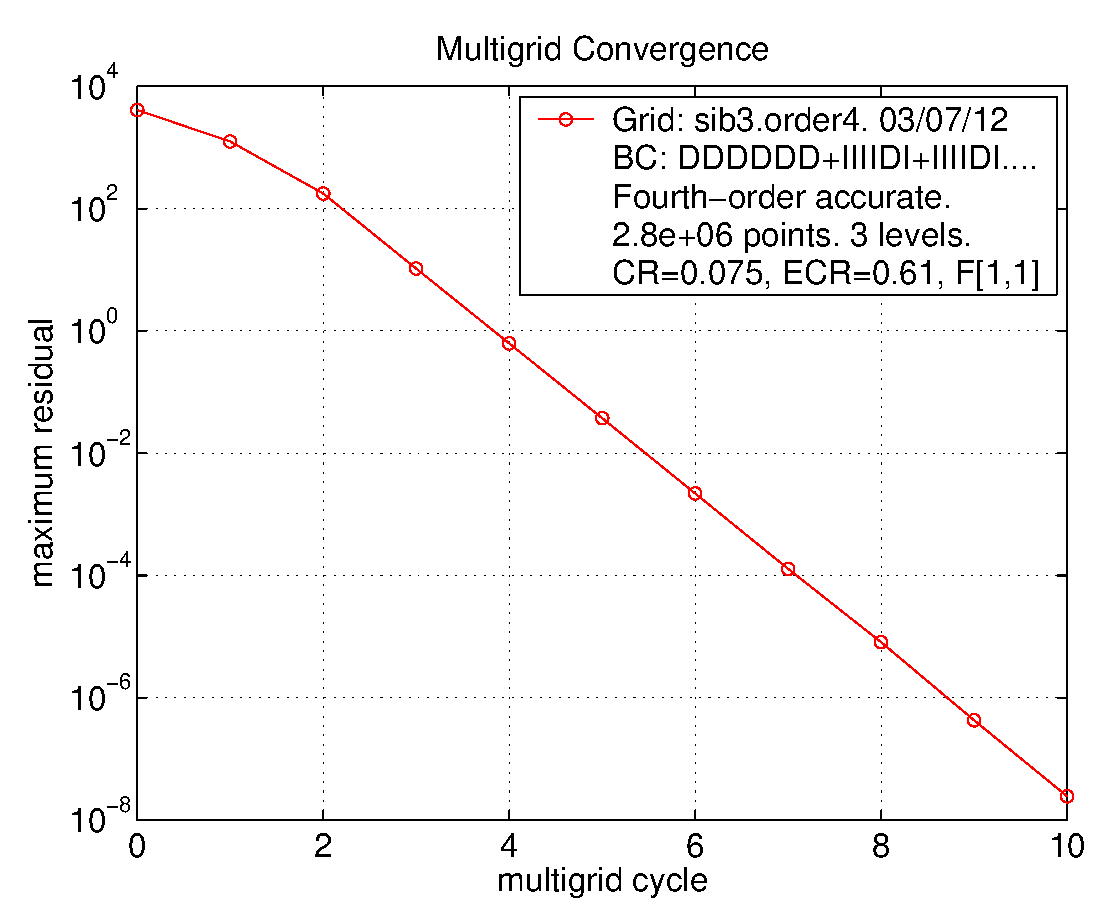
\epsfig{file=residual.sib3.order4.eps,width=\figWidth}
%- 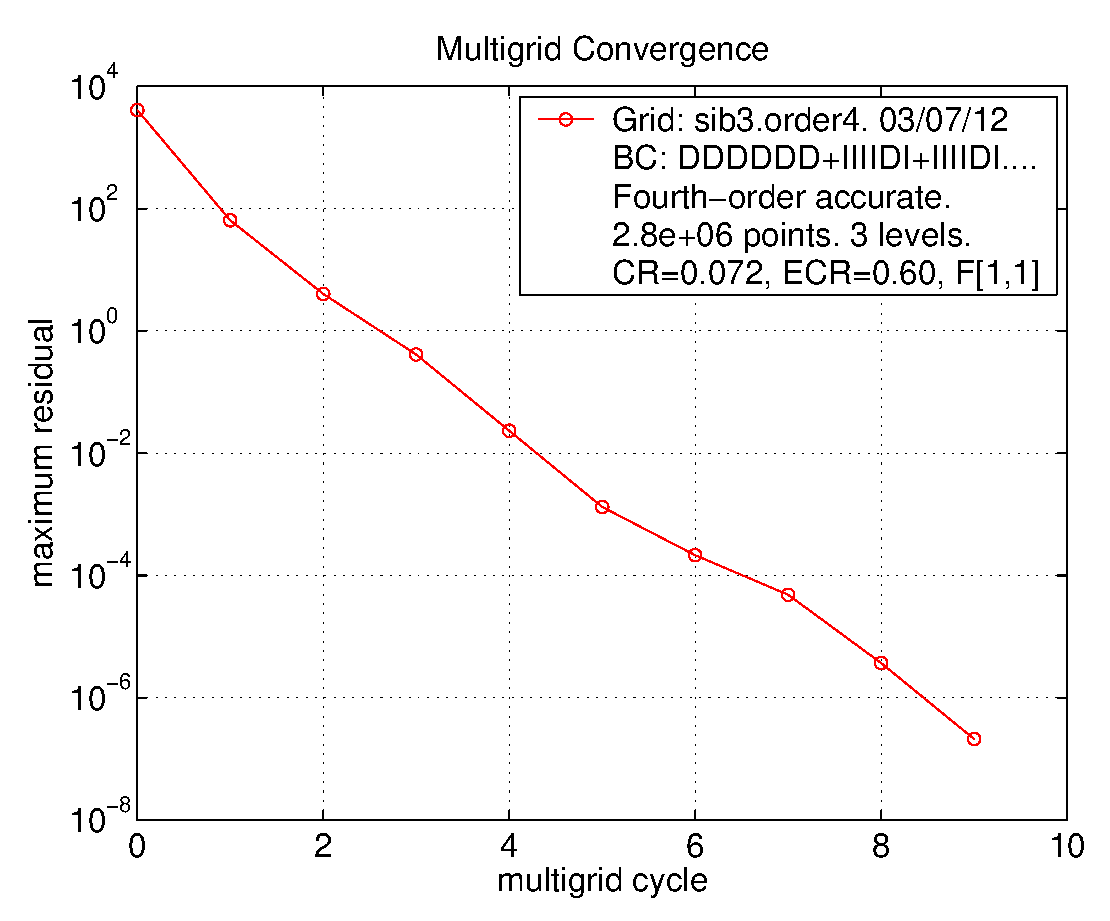
\epsfig{file=residual.sib3.order4.fmg.eps,width=\figWidth}
%- 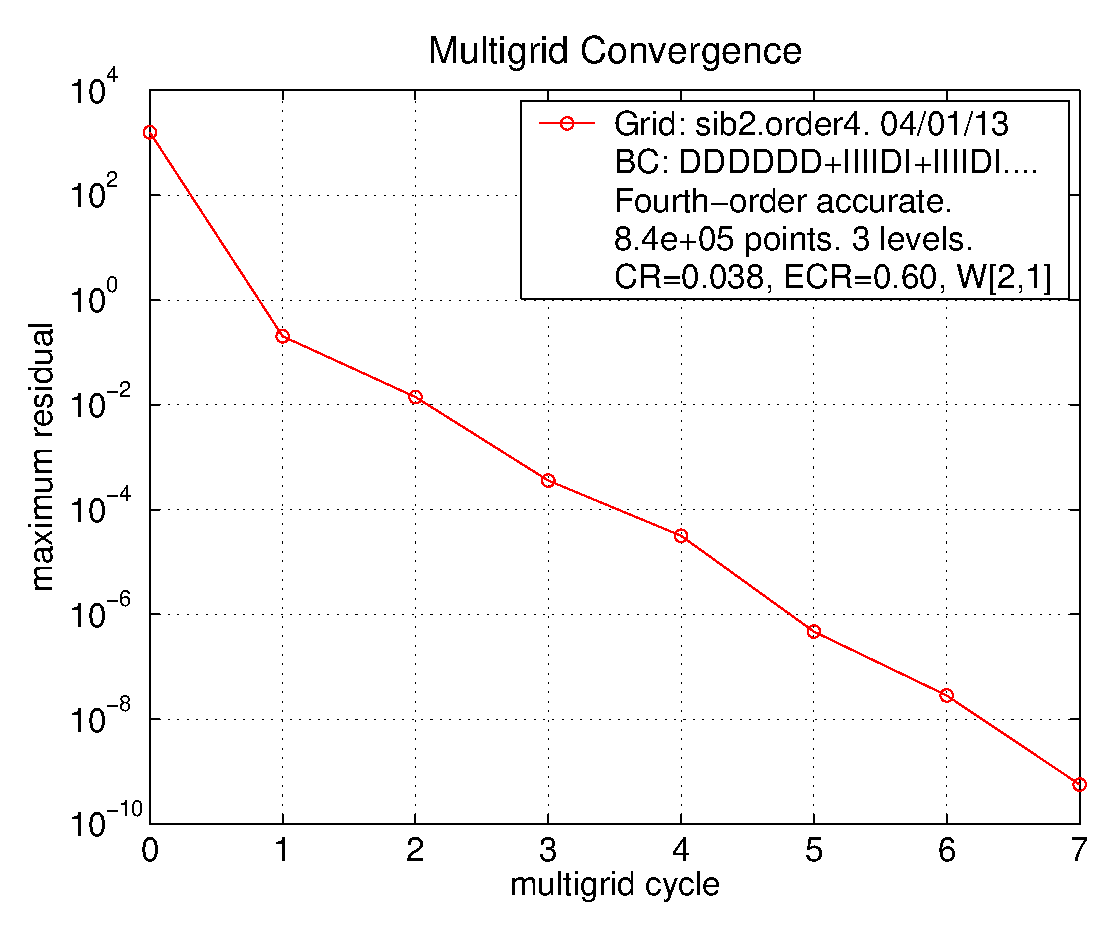
\epsfig{file=residual.sib2.order4.eps,width=\figWidth}
%- \end{center}
%- \caption{Convergence history for a sphere in a box, fourth-order. Right: Full multigrid.}
%- \label{fig:sib3.order4}
%- \end{figure}

\begin{table}[hbt]
\begin{center}
{\tablefontsize
\begin{tabular}{|c|c|c|c|c|} \hline 
 $i$   & $\vert\vert\mbox{res}\vert\vert_\infty$  &  CR     &  WU    & ECR  \\   \hline 
 $ 1$  & $ 6.4e+02$ & $0.156$ & $ 8.8$ & $0.81$ \\ 
 $ 2$  & $ 2.8e+01$ & $0.044$ & $ 6.3$ & $0.61$ \\ 
 $ 3$  & $ 6.1e-01$ & $0.022$ & $ 6.5$ & $0.56$ \\ 
 $ 4$  & $ 2.8e-02$ & $0.046$ & $ 7.0$ & $0.64$ \\ 
 $ 5$  & $ 1.2e-03$ & $0.041$ & $ 7.3$ & $0.64$ \\ 
 $ 6$  & $ 4.8e-05$ & $0.042$ & $ 7.3$ & $0.65$ \\ 
 $ 7$  & $ 2.0e-06$ & $0.042$ & $ 7.3$ & $0.65$ \\ 
 $ 8$  & $ 8.3e-08$ & $0.041$ & $ 6.8$ & $0.62$ \\ 
\hline 
\multicolumn{5}{|c|}{Grid: sib3.order4. 03/07/12}  \\
\multicolumn{5}{|c|}{BC: DDDDDD+IIIIDI+IIIIDI....}  \\
\multicolumn{5}{|c|}{Fourth-order accurate. NO-OP-AVE}  \\
\multicolumn{5}{|c|}{Trigonometric solution.}  \\
\multicolumn{5}{|c|}{W[2,1]: rb $\omega=1.20$, lz3 $\omega=1.00$}  \\
\multicolumn{5}{|c|}{2.78e+06 grid-points. 3 levels.}  \\
\multicolumn{5}{|c|}{Average CR=$0.046$, ECR=$0.65$.}  \\
\multicolumn{5}{|c|}{time/cycle = 1.70e+01 s.}  \\
\hline 
\end{tabular}
\begin{tabular}{|c|c|c|c|c|} \hline 
 $i$   & $\vert\vert\mbox{res}\vert\vert_\infty$  &  CR     &  WU    & ECR  \\   \hline 
 $ 1$  & $ 5.9e+02$ & $0.144$ & $ 8.8$ & $0.80$ \\ 
 $ 2$  & $ 2.6e+01$ & $0.044$ & $ 6.3$ & $0.61$ \\ 
 $ 3$  & $ 4.4e-01$ & $0.017$ & $ 6.5$ & $0.54$ \\ 
 $ 4$  & $ 7.8e-03$ & $0.018$ & $ 6.5$ & $0.54$ \\ 
 $ 5$  & $ 4.1e-04$ & $0.052$ & $ 7.0$ & $0.66$ \\ 
 $ 6$  & $ 1.1e-05$ & $0.027$ & $ 7.3$ & $0.61$ \\ 
 $ 7$  & $ 1.4e-06$ & $0.129$ & $ 7.3$ & $0.75$ \\ 
 $ 8$  & $ 8.1e-08$ & $0.057$ & $ 7.3$ & $0.67$ \\ 
\hline 
\multicolumn{5}{|c|}{Grid: sib3.order4. 03/07/12}  \\
\multicolumn{5}{|c|}{BC: DDDDDD+IIIIDI+IIIIDI....}  \\
\multicolumn{5}{|c|}{Fourth-order accurate. IBS541}  \\
\multicolumn{5}{|c|}{Trigonometric solution.}  \\
\multicolumn{5}{|c|}{F[2,1]: rb $\omega=1.20$, lz3 $\omega=1.00$}  \\
\multicolumn{5}{|c|}{2.78e+06 grid-points. 3 levels.}  \\
\multicolumn{5}{|c|}{Average CR=$0.046$, ECR=$0.65$.}  \\
\multicolumn{5}{|c|}{time/cycle = 1.74e+01 s.}  \\
\hline 
\end{tabular}
\begin{tabular}{|c|c|c|c|c|} \hline 
 $i$   & $\vert\vert\mbox{res}\vert\vert_\infty$  &  CR     &  WU    & ECR  \\   \hline 
 $ 1$  & $ 1.2e+03$ & $0.284$ & $ 6.5$ & $0.82$ \\ 
 $ 2$  & $ 1.5e+02$ & $0.131$ & $ 4.7$ & $0.65$ \\ 
 $ 3$  & $ 7.8e+00$ & $0.052$ & $ 5.0$ & $0.55$ \\ 
 $ 4$  & $ 4.0e-01$ & $0.051$ & $ 5.0$ & $0.55$ \\ 
 $ 5$  & $ 2.1e-02$ & $0.051$ & $ 5.2$ & $0.57$ \\ 
 $ 6$  & $ 1.0e-03$ & $0.051$ & $ 5.0$ & $0.55$ \\ 
 $ 7$  & $ 5.2e-05$ & $0.050$ & $ 5.0$ & $0.55$ \\ 
 $ 8$  & $ 8.0e-06$ & $0.152$ & $ 4.7$ & $0.67$ \\ 
% $ 9$  & $ 1.7e-06$ & $0.210$ & $ 4.6$ & $0.71$ \\ 
% $10$  & $ 1.1e-07$ & $0.067$ & $ 4.9$ & $0.58$ \\ 
\hline 
\multicolumn{5}{|c|}{Grid: sib3.order4. 03/07/12}  \\
\multicolumn{5}{|c|}{BC: DDDDDD+IIIIDI+IIIIDI....}  \\
\multicolumn{5}{|c|}{Fourth-order accurate. IBS641}  \\
\multicolumn{5}{|c|}{Trigonometric solution.}  \\
\multicolumn{5}{|c|}{F[1,1]: rb $\omega=1.20$, lz3 $\omega=1.00$}  \\
\multicolumn{5}{|c|}{2.78e+06 grid-points. 3 levels.}  \\
\multicolumn{5}{|c|}{Average CR=$0.088$, ECR=$0.62$.}  \\
\multicolumn{5}{|c|}{time/cycle = 1.21e+01 s.}  \\
\hline 
\end{tabular}
\begin{tabular}{|c|c|c|c|c|} \hline 
 $i$   & $\vert\vert\mbox{res}\vert\vert_\infty$  &  CR     &  WU    & ECR  \\   \hline 
 $ 1$  & $ 1.3e+03$ & $0.308$ & $ 6.5$ & $0.83$ \\ 
 $ 2$  & $ 1.8e+02$ & $0.140$ & $ 4.7$ & $0.66$ \\ 
 $ 3$  & $ 1.0e+01$ & $0.059$ & $ 5.0$ & $0.57$ \\ 
 $ 4$  & $ 6.3e-01$ & $0.060$ & $ 5.2$ & $0.58$ \\ 
 $ 5$  & $ 3.7e-02$ & $0.060$ & $ 5.1$ & $0.57$ \\ 
 $ 6$  & $ 2.2e-03$ & $0.059$ & $ 5.0$ & $0.57$ \\ 
 $ 7$  & $ 1.3e-04$ & $0.058$ & $ 5.0$ & $0.56$ \\ 
 $ 8$  & $ 8.1e-06$ & $0.064$ & $ 5.0$ & $0.57$ \\ 
% $ 9$  & $ 4.3e-07$ & $0.052$ & $ 5.2$ & $0.57$ \\ 
% $10$  & $ 2.4e-08$ & $0.057$ & $ 5.0$ & $0.57$ \\ 
\hline 
\multicolumn{5}{|c|}{Grid: sib3.order4. 03/07/12}  \\
\multicolumn{5}{|c|}{BC: DDDDDD+IIIIDI+IIIIDI....}  \\
\multicolumn{5}{|c|}{Fourth-order accurate. IBS541 }  \\
\multicolumn{5}{|c|}{Trigonometric solution.}  \\
\multicolumn{5}{|c|}{F[1,1]: rb $\omega=1.20$, lz3 $\omega=1.00$}  \\
\multicolumn{5}{|c|}{2.78e+06 grid-points. 3 levels.}  \\
\multicolumn{5}{|c|}{Average CR=$0.075$, ECR=$0.61$.}  \\
\multicolumn{5}{|c|}{time/cycle = 1.21e+01 s.}  \\
\hline 
\end{tabular}
\begin{tabular}{|c|c|c|c|c|} \hline 
 $i$   & $\vert\vert\mbox{res}\vert\vert_\infty$  &  CR     &  WU    & ECR  \\   \hline 
 $ 1$  & $ 1.3e+03$ & $0.324$ & $ 6.5$ & $0.84$ \\ 
 $ 2$  & $ 2.1e+02$ & $0.156$ & $ 4.7$ & $0.67$ \\ 
 $ 3$  & $ 1.4e+01$ & $0.067$ & $ 5.0$ & $0.58$ \\ 
 $ 4$  & $ 9.5e-01$ & $0.069$ & $ 5.2$ & $0.60$ \\ 
 $ 5$  & $ 6.5e-02$ & $0.068$ & $ 5.1$ & $0.59$ \\ 
 $ 6$  & $ 4.4e-03$ & $0.068$ & $ 5.0$ & $0.58$ \\ 
 $ 7$  & $ 2.9e-04$ & $0.067$ & $ 5.0$ & $0.58$ \\ 
 $ 8$  & $ 2.0e-05$ & $0.067$ & $ 5.2$ & $0.60$ \\ 
% $ 9$  & $ 1.3e-06$ & $0.066$ & $ 5.1$ & $0.58$ \\ 
% $10$  & $ 8.6e-08$ & $0.066$ & $ 5.0$ & $0.58$ \\ 
\hline 
\multicolumn{5}{|c|}{Grid: sib3.order4. 03/07/12}  \\
\multicolumn{5}{|c|}{BC: DDDDDD+IIIIDI+IIIIDI....}  \\
\multicolumn{5}{|c|}{Fourth-order accurate. IBS431}  \\
\multicolumn{5}{|c|}{Trigonometric solution.}  \\
\multicolumn{5}{|c|}{F[1,1]: rb $\omega=1.20$, lz3 $\omega=1.00$}  \\
\multicolumn{5}{|c|}{2.78e+06 grid-points. 3 levels.}  \\
\multicolumn{5}{|c|}{Average CR=$0.086$, ECR=$0.62$.}  \\
\multicolumn{5}{|c|}{time/cycle = 1.14e+01 s.}  \\
\hline 
\end{tabular}
\begin{tabular}{|c|c|c|c|c|} \hline 
 $i$   & $\vert\vert\mbox{res}\vert\vert_\infty$  &  CR     &  WU    & ECR  \\   \hline 
 $ 1$  & $ 1.5e+02$ & $0.037$ & $ 6.5$ & $0.60$ \\ 
 $ 2$  & $ 1.7e+01$ & $0.113$ & $ 4.5$ & $0.62$ \\ 
 $ 3$  & $ 8.1e-01$ & $0.047$ & $ 4.7$ & $0.52$ \\ 
 $ 4$  & $ 4.5e-02$ & $0.055$ & $ 5.0$ & $0.56$ \\ 
 $ 5$  & $ 3.7e-03$ & $0.084$ & $ 5.2$ & $0.62$ \\ 
 $ 6$  & $ 3.3e-04$ & $0.089$ & $ 5.5$ & $0.64$ \\ 
 $ 7$  & $ 2.4e-05$ & $0.072$ & $ 5.5$ & $0.62$ \\ 
 $ 8$  & $ 2.1e-06$ & $0.086$ & $ 5.5$ & $0.64$ \\ 
% $ 9$  & $ 2.0e-07$ & $0.097$ & $ 5.5$ & $0.65$ \\ 
% $10$  & $ 1.7e-08$ & $0.087$ & $ 5.5$ & $0.64$ \\ 
\hline 
\multicolumn{5}{|c|}{Grid: sib3.order4. 03/07/12}  \\
\multicolumn{5}{|c|}{BC: DDDDDD+IIIIDI+IIIIDI....}  \\
\multicolumn{5}{|c|}{4th-order accurate. PBS431 IBS431}  \\
\multicolumn{5}{|c|}{Trigonometric solution.}  \\
\multicolumn{5}{|c|}{F[1,1]: rb $\omega=1.20$, lz3 $\omega=1.00$}  \\
\multicolumn{5}{|c|}{2.78e+06 grid-points. 3 levels.}  \\
\multicolumn{5}{|c|}{Average CR=$0.073$, ECR=$0.61$.}  \\
\multicolumn{5}{|c|}{time/cycle = 1.36e+01 s.}  \\
\hline 
\end{tabular}
\begin{tabular}{|c|c|c|c|c|} \hline 
 $i$   & $\vert\vert\mbox{res}\vert\vert_\infty$  &  CR     &  WU    & ECR  \\   \hline 
 $ 1$  & $ 6.4e+02$ & $0.157$ & $ 8.8$ & $0.81$ \\ 
 $ 2$  & $ 3.3e+01$ & $0.051$ & $ 6.3$ & $0.62$ \\ 
 $ 3$  & $ 6.4e-01$ & $0.020$ & $ 6.5$ & $0.55$ \\ 
 $ 4$  & $ 1.4e-02$ & $0.022$ & $ 7.0$ & $0.58$ \\ 
 $ 5$  & $ 1.0e-03$ & $0.073$ & $ 7.3$ & $0.70$ \\ 
 $ 6$  & $ 6.2e-05$ & $0.061$ & $ 7.3$ & $0.68$ \\ 
 $ 7$  & $ 2.4e-06$ & $0.039$ & $ 7.3$ & $0.64$ \\ 
 $ 8$  & $ 5.4e-08$ & $0.022$ & $ 7.3$ & $0.59$ \\ 
% $ 9$  & $ 9.3e-09$ & $0.173$ & $ 7.3$ & $0.79$ \\ 
% $10$  & $ 8.2e-10$ & $0.088$ & $ 7.3$ & $0.72$ \\ 
\hline 
\multicolumn{5}{|c|}{Grid: sib3.order4. 03/07/12}  \\
\multicolumn{5}{|c|}{BC: DDDDDD+IIIIDI+IIIIDI....}  \\
\multicolumn{5}{|c|}{Fourth-order accurate.}  \\
\multicolumn{5}{|c|}{Trigonometric solution.}  \\
\multicolumn{5}{|c|}{W[2,1]: rb $\omega=1.20$, lz3 $\omega=1.00$}  \\
\multicolumn{5}{|c|}{2.78e+06 grid-points. 3 levels.}  \\
\multicolumn{5}{|c|}{Average CR=$0.054$, ECR=$0.67$.}  \\
\multicolumn{5}{|c|}{time/cycle = 1.58e+01 s.}  \\
\hline 
\end{tabular}
\begin{tabular}{|c|c|c|c|c|} \hline 
 $i$   & $\vert\vert\mbox{res}\vert\vert_\infty$  &  CR     &  WU    & ECR  \\   \hline 
 $ 1$  & $ 3.4e+02$ & $0.082$ & $ 8.8$ & $0.75$ \\ 
 $ 2$  & $ 4.8e+00$ & $0.014$ & $ 6.3$ & $0.51$ \\ 
 $ 3$  & $ 1.3e-01$ & $0.027$ & $ 7.5$ & $0.62$ \\ 
 $ 4$  & $ 4.9e-03$ & $0.037$ & $ 8.9$ & $0.69$ \\ 
 $ 5$  & $ 3.3e-04$ & $0.068$ & $ 9.8$ & $0.76$ \\ 
 $ 6$  & $ 1.4e-05$ & $0.042$ & $10.1$ & $0.73$ \\ 
 $ 7$  & $ 4.7e-07$ & $0.035$ & $10.1$ & $0.72$ \\ 
 $ 8$  & $ 2.0e-08$ & $0.042$ & $10.1$ & $0.73$ \\ 
% $ 9$  & $ 1.7e-09$ & $0.086$ & $10.1$ & $0.78$ \\ 
\hline 
\multicolumn{5}{|c|}{Grid: sib3.order4. 03/07/12}  \\
\multicolumn{5}{|c|}{BC: DDDDDD+IIIIDI+IIIIDI....}  \\
\multicolumn{5}{|c|}{Fourth-order accurate.}  \\
\multicolumn{5}{|c|}{Trigonometric solution.}  \\
\multicolumn{5}{|c|}{F[2,1]: rb $\omega=1.20$}  \\
\multicolumn{5}{|c|}{2.78e+06 grid-points. 3 levels.}  \\
\multicolumn{5}{|c|}{Average CR=$0.042$, ECR=$0.71$.}  \\
\multicolumn{5}{|c|}{time/cycle = 1.95e+01 s.}  \\
\hline 
\end{tabular}
\begin{tabular}{|c|c|c|c|c|} \hline 
 $i$   & $\vert\vert\mbox{res}\vert\vert_\infty$  &  CR     &  WU    & ECR  \\   \hline 
 $ 1$  & $ 2.5e+00$ & $0.043$ & $ 6.1$ & $0.60$ \\ 
 $ 2$  & $ 1.4e-01$ & $0.056$ & $ 7.5$ & $0.68$ \\ 
 $ 3$  & $ 5.4e-03$ & $0.039$ & $ 8.9$ & $0.69$ \\ 
 $ 4$  & $ 2.1e-04$ & $0.038$ & $ 9.3$ & $0.70$ \\ 
 $ 5$  & $ 2.5e-05$ & $0.120$ & $ 9.3$ & $0.80$ \\ 
 $ 6$  & $ 1.7e-06$ & $0.067$ & $ 9.3$ & $0.75$ \\ 
 $ 7$  & $ 1.1e-07$ & $0.064$ & $ 9.3$ & $0.74$ \\ 
 $ 8$  & $ 5.7e-09$ & $0.053$ & $ 9.3$ & $0.73$ \\ 
\hline 
\multicolumn{5}{|c|}{Grid: sib3.order4. 03/06/18}  \\
\multicolumn{5}{|c|}{BC: DDDDDD+IIIIDI+IIIIDI....}  \\
\multicolumn{5}{|c|}{Fourth-order accurate.}  \\
\multicolumn{5}{|c|}{Trigonometric solution. IBS+PBS}  \\
\multicolumn{5}{|c|}{W[2,1]: rb $\omega=1.20$}  \\
\multicolumn{5}{|c|}{2.78e+06 grid-points. 3 levels.}  \\
\multicolumn{5}{|c|}{Average CR=$0.056$, ECR=$0.72$.}  \\
\multicolumn{5}{|c|}{time/cycle = 2.29e+01 s.}  \\
\hline 
\end{tabular}
\begin{tabular}{|c|c|c|c|c|} \hline 
 $i$   & res      & rate    &  WU    & ECR  \\   \hline 
 $ 1$  & $ 6.0e+01$ & $0.034$ & $ 5.4$ & $0.53$ \\ 
 $ 2$  & $ 2.9e+00$ & $0.048$ & $ 6.8$ & $0.64$ \\ 
 $ 3$  & $ 5.3e-01$ & $0.186$ & $ 8.2$ & $0.81$ \\ 
 $ 4$  & $ 7.5e-02$ & $0.141$ & $ 8.9$ & $0.80$ \\ 
 $ 5$  & $ 9.8e-03$ & $0.131$ & $ 8.9$ & $0.80$ \\ 
 $ 6$  & $ 1.3e-03$ & $0.131$ & $ 8.9$ & $0.80$ \\ 
 $ 7$  & $ 1.7e-04$ & $0.134$ & $ 8.9$ & $0.80$ \\ 
\hline 
\multicolumn{5}{|c|}{Grid: sib3.order4.}  \\
\multicolumn{5}{|c|}{Dirichlet boundary conditions.}  \\
\multicolumn{5}{|c|}{Fourth-order accurate.}  \\
\multicolumn{5}{|c|}{Trigonometric solution.}  \\
\multicolumn{5}{|c|}{Smoother rb[2,1] $\omega=1.20$}  \\
\multicolumn{5}{|c|}{2.78e+06 grid-points. 3 levels.}  \\
\multicolumn{5}{|c|}{Average CR=$0.100$, ECR=$0.75$.}  \\
\multicolumn{5}{|c|}{time/cycle = 1.62e+01 s.}  \\
\hline 
\end{tabular}
} % end \tablefontsize
\end{center}
\caption{Multigrid convergence rates for a sphere-in-a-box, fourth-order accuracy.}
\label{fig:sibII}
\end{table}


\begin{table}[hbt]
\begin{center}
{\tablefontsize
\begin{tabular}{|c|c|c|c|c|} \hline 
 $i$   & $\vert\vert\mbox{res}\vert\vert_\infty$  &  CR     &  WU    & ECR  \\   \hline 
 $ 1$  & $ 2.2e+02$ & $0.139$ & $ 8.8$ & $0.80$ \\ 
 $ 2$  & $ 6.3e+00$ & $0.028$ & $ 6.7$ & $0.59$ \\ 
 $ 3$  & $ 9.4e-02$ & $0.015$ & $ 7.1$ & $0.55$ \\ 
 $ 4$  & $ 2.4e-03$ & $0.025$ & $ 7.1$ & $0.59$ \\ 
 $ 5$  & $ 7.4e-05$ & $0.031$ & $ 7.1$ & $0.61$ \\ 
 $ 6$  & $ 2.2e-06$ & $0.029$ & $ 7.9$ & $0.64$ \\ 
 $ 7$  & $ 6.9e-08$ & $0.032$ & $ 7.5$ & $0.63$ \\ 
 $ 8$  & $ 2.2e-09$ & $0.032$ & $ 7.1$ & $0.62$ \\ 
\hline 
\multicolumn{5}{|c|}{Grid: sib2.order4. 03/07/12}  \\
\multicolumn{5}{|c|}{BC: DDDDDD+IIIIDI+IIIIDI....}  \\
\multicolumn{5}{|c|}{Fourth-order accurate.NO-OP-AVE}  \\
\multicolumn{5}{|c|}{Trigonometric solution.}  \\
\multicolumn{5}{|c|}{W[2,1]: rb $\omega=1.20$, lz3 $\omega=1.00$}  \\
\multicolumn{5}{|c|}{8.25e+05 grid-points. 3 levels.}  \\
\multicolumn{5}{|c|}{Average CR=$0.033$, ECR=$0.63$.}  \\
\multicolumn{5}{|c|}{time/cycle = 5.88e+00 s.}  \\
\hline 
\end{tabular}
\begin{tabular}{|c|c|c|c|c|} \hline 
 $i$   & $\vert\vert\mbox{res}\vert\vert_\infty$  &  CR     &  WU    & ECR  \\   \hline 
 $ 1$  & $ 1.1e+02$ & $0.069$ & $ 8.8$ & $0.74$ \\ 
 $ 2$  & $ 1.2e+00$ & $0.011$ & $ 6.8$ & $0.51$ \\ 
 $ 3$  & $ 3.9e-02$ & $0.033$ & $ 8.7$ & $0.68$ \\ 
 $ 4$  & $ 1.2e-03$ & $0.031$ & $11.0$ & $0.73$ \\ 
 $ 5$  & $ 3.2e-05$ & $0.027$ & $12.6$ & $0.75$ \\ 
 $ 6$  & $ 6.7e-07$ & $0.021$ & $13.0$ & $0.74$ \\ 
 $ 7$  & $ 1.4e-08$ & $0.021$ & $12.2$ & $0.73$ \\ 
\hline 
\multicolumn{5}{|c|}{Grid: sib2.order4. 03/07/12}  \\
\multicolumn{5}{|c|}{BC: DDDDDD+IIIIDI+IIIIDI....}  \\
\multicolumn{5}{|c|}{Fourth-order accurate. NO-OP-AVE}  \\
\multicolumn{5}{|c|}{Trigonometric solution.}  \\
\multicolumn{5}{|c|}{W[2,1]: rb $\omega=1.19$}  \\
\multicolumn{5}{|c|}{8.25e+05 grid-points. 3 levels.}  \\
\multicolumn{5}{|c|}{Average CR=$0.026$, ECR=$0.71$.}  \\
\multicolumn{5}{|c|}{time/cycle = 7.52e+00 s.}  \\
\hline 
\end{tabular}
\begin{tabular}{|c|c|c|c|c|} \hline 
 $i$   & $\vert\vert\mbox{res}\vert\vert_\infty$  &  CR     &  WU    & ECR  \\   \hline 
 $ 1$  & $ 6.5e+01$ & $0.016$ & $ 7.4$ & $0.57$ \\ 
 $ 2$  & $ 4.0e+00$ & $0.062$ & $ 4.7$ & $0.56$ \\ 
 $ 3$  & $ 4.1e-01$ & $0.102$ & $ 4.8$ & $0.62$ \\ 
 $ 4$  & $ 2.3e-02$ & $0.057$ & $ 5.0$ & $0.56$ \\ 
 $ 5$  & $ 1.3e-03$ & $0.057$ & $ 5.0$ & $0.56$ \\ 
 $ 6$  & $ 2.1e-04$ & $0.162$ & $ 4.7$ & $0.68$ \\ 
 $ 7$  & $ 4.8e-05$ & $0.226$ & $ 4.6$ & $0.72$ \\ 
 $ 8$  & $ 3.7e-06$ & $0.077$ & $ 4.9$ & $0.59$ \\ 
 $ 9$  & $ 2.1e-07$ & $0.057$ & $ 5.2$ & $0.58$ \\ 
\hline 
\multicolumn{5}{|c|}{Grid: sib3.order4. 03/07/12}  \\
\multicolumn{5}{|c|}{BC: DDDDDD+IIIIDI+IIIIDI....}  \\
\multicolumn{5}{|c|}{Fourth-order accurate.}  \\
\multicolumn{5}{|c|}{Trigonometric solution.}  \\
\multicolumn{5}{|c|}{Full Multigrid.}  \\
\multicolumn{5}{|c|}{F[1,1]: rb $\omega=1.20$, lz3 $\omega=1.00$}  \\
\multicolumn{5}{|c|}{2.78e+06 grid-points. 3 levels.}  \\
\multicolumn{5}{|c|}{Average CR=$0.072$, ECR=$0.60$.}  \\
\multicolumn{5}{|c|}{time/cycle = 1.24e+01 s.}  \\
\hline 
\end{tabular}
\begin{tabular}{|c|c|c|c|c|} \hline 
 $i$   & $\vert\vert\mbox{res}\vert\vert_\infty$  &  CR     &  WU    & ECR  \\   \hline 
 $ 1$  & $ 3.3e+01$ & $0.008$ & $10.4$ & $0.63$ \\ 
 $ 2$  & $ 1.8e+00$ & $0.054$ & $ 6.9$ & $0.65$ \\ 
 $ 3$  & $ 1.1e-01$ & $0.064$ & $ 6.9$ & $0.67$ \\ 
 $ 4$  & $ 1.6e-03$ & $0.014$ & $ 8.4$ & $0.60$ \\ 
 $ 5$  & $ 2.2e-05$ & $0.014$ & $ 9.1$ & $0.62$ \\ 
 $ 6$  & $ 8.8e-07$ & $0.040$ & $ 7.5$ & $0.65$ \\ 
 $ 7$  & $ 3.6e-08$ & $0.040$ & $ 6.8$ & $0.62$ \\ 
\hline 
\multicolumn{5}{|c|}{Grid: sib3.order4. 03/07/12}  \\
\multicolumn{5}{|c|}{BC: DDDDDD+IIIIDI+IIIIDI....}  \\
\multicolumn{5}{|c|}{Fourth-order accurate.}  \\
\multicolumn{5}{|c|}{Trigonometric solution.}  \\
\multicolumn{5}{|c|}{F[2,1]: rb $\omega=1.20$, alz $\omega=1.00$}  \\
\multicolumn{5}{|c|}{2.78e+06 grid-points. 3 levels.}  \\
\multicolumn{5}{|c|}{Average CR=$0.026$, ECR=$0.63$.}  \\
\multicolumn{5}{|c|}{time/cycle = 1.93e+01 s.}  \\
\hline 
\end{tabular}
\begin{tabular}{|c|c|c|c|c|} \hline 
 $i$   & $\vert\vert\mbox{res}\vert\vert_\infty$  &  CR     &  WU    & ECR  \\   \hline 
 $ 1$  & $ 1.6e+01$ & $0.010$ & $ 7.4$ & $0.54$ \\ 
 $ 2$  & $ 2.5e+00$ & $0.151$ & $ 4.5$ & $0.66$ \\ 
 $ 3$  & $ 2.1e-01$ & $0.084$ & $ 4.9$ & $0.61$ \\ 
 $ 4$  & $ 2.6e-02$ & $0.126$ & $ 5.3$ & $0.68$ \\ 
 $ 5$  & $ 3.9e-03$ & $0.152$ & $ 5.7$ & $0.72$ \\ 
 $ 6$  & $ 6.5e-04$ & $0.165$ & $ 6.1$ & $0.75$ \\ 
 $ 7$  & $ 1.1e-04$ & $0.162$ & $ 6.1$ & $0.74$ \\ 
 $ 8$  & $ 1.8e-05$ & $0.174$ & $ 6.1$ & $0.75$ \\ 
% $ 9$  & $ 3.0e-06$ & $0.164$ & $ 6.1$ & $0.75$ \\ 
% $10$  & $ 5.3e-07$ & $0.175$ & $ 6.1$ & $0.75$ \\ 
\hline 
\multicolumn{5}{|c|}{Grid: sib2.order4. 03/07/12}  \\
\multicolumn{5}{|c|}{BC: DDDDDD+IIIIDI+IIIIDI....}  \\
\multicolumn{5}{|c|}{Fourth-order accurate.}  \\
\multicolumn{5}{|c|}{Trigonometric solution.}  \\
\multicolumn{5}{|c|}{Full Multigrid.}  \\
\multicolumn{5}{|c|}{F[1,1]: rb $\omega=1.20$, lz3 $\omega=1.00$}  \\
\multicolumn{5}{|c|}{8.25e+05 grid-points. 3 levels.}  \\
\multicolumn{5}{|c|}{Average CR=$0.113$, ECR=$0.69$.}  \\
\multicolumn{5}{|c|}{time/cycle = 4.96e+00 s.}  \\
\hline 
\end{tabular}
\begin{tabular}{|c|c|c|c|c|} \hline 
 $i$   & $\vert\vert\mbox{res}\vert\vert_\infty$  &  CR     &  WU    & ECR  \\   \hline 
 $ 1$  & $ 4.0e+02$ & $0.252$ & $ 6.5$ & $0.81$ \\ 
 $ 2$  & $ 3.6e+01$ & $0.090$ & $ 4.9$ & $0.61$ \\ 
 $ 3$  & $ 1.3e+00$ & $0.035$ & $ 5.3$ & $0.53$ \\ 
 $ 4$  & $ 6.2e-02$ & $0.049$ & $ 5.3$ & $0.57$ \\ 
 $ 5$  & $ 1.1e-02$ & $0.170$ & $ 5.3$ & $0.72$ \\ 
 $ 6$  & $ 1.8e-03$ & $0.173$ & $ 5.7$ & $0.74$ \\ 
 $ 7$  & $ 3.1e-04$ & $0.167$ & $ 6.1$ & $0.75$ \\ 
 $ 8$  & $ 5.2e-05$ & $0.170$ & $ 6.1$ & $0.75$ \\ 
% $ 9$  & $ 8.4e-06$ & $0.162$ & $ 6.1$ & $0.74$ \\ 
% $10$  & $ 1.5e-06$ & $0.174$ & $ 6.1$ & $0.75$ \\ 
\hline 
\multicolumn{5}{|c|}{Grid: sib2.order4. 03/07/12}  \\
\multicolumn{5}{|c|}{BC: DDDDDD+IIIIDI+IIIIDI....}  \\
\multicolumn{5}{|c|}{Fourth-order accurate.}  \\
\multicolumn{5}{|c|}{Trigonometric solution.}  \\
\multicolumn{5}{|c|}{F[1,1]: rb $\omega=1.20$, lz3 $\omega=1.00$}  \\
\multicolumn{5}{|c|}{8.25e+05 grid-points. 3 levels.}  \\
\multicolumn{5}{|c|}{Average CR=$0.125$, ECR=$0.70$.}  \\
\multicolumn{5}{|c|}{time/cycle = 4.86e+00 s.}  \\
\hline 
\end{tabular}
} % end \tablefontsize
\end{center}
\caption{Multigrid convergence rates for a sphere-in-a-box, fourth-order accuracy.}
\label{fig:sibII}
\end{table}



% ========================= OLD SIB =========================================


% 
% \begin{table}[hbt]
% \begin{center}
% \begin{tabular}{|c|c|c|c|c|}                   \hline
%  $i$   & res(i)     & rate(i)    &  WU(i)     & ECR(i)  \\   \hline
%  $ 1$  & $ 5.7e+00$ & $0.088$ & $ 6.1$ & $0.67$ \\ 
%  $ 2$  & $ 4.5e-01$ & $0.079$ & $ 6.1$ & $0.66$ \\ 
%  $ 3$  & $ 3.6e-02$ & $0.081$ & $ 6.1$ & $0.66$ \\ 
%  $ 4$  & $ 3.9e-03$ & $0.108$ & $ 6.1$ & $0.69$ \\ 
%  $ 5$  & $ 7.7e-04$ & $0.197$ & $ 5.6$ & $0.75$ \\ 
%  $ 6$  & $ 1.5e-04$ & $0.199$ & $ 5.4$ & $0.74$ \\ 
%  $ 7$  & $ 2.7e-05$ & $0.176$ & $ 5.1$ & $0.71$ \\ 
%  $ 8$  & $ 5.4e-06$ & $0.201$ & $ 5.5$ & $0.75$ \\ 
%  $ 9$  & $ 9.5e-07$ & $0.175$ & $ 5.1$ & $0.71$ \\ 
%  $10$  & $ 1.8e-07$ & $0.192$ & $ 5.6$ & $0.74$ \\ 
%  \hline
%  \multicolumn{5}{c}{Red-Black, sibmg}         \\
%  \multicolumn{5}{c}{2 levels, Dirichlet}         \\
% \end{tabular}
% \end{center}
% \caption{Multigrid convergence rates for a 3D sphere in a box.}
% \label{fig:smoothSib}
% \end{table}


% \begin{tabular}{|c|c|c|c|}                   \hline
%  $i$   & res(i)    & $W(i)$  & ECR(i) \\   \hline
%  $1$   & $$ & $$   & $$  \\
%  $2$   & $$ & $$   & $$  \\
%  $3$   & $$ & $$   & $$  \\
%  $4$   & $$ & $$   & $$  \\
%  $5$   & $$ & $$   & $$  \\   \hline
%  \multicolumn{4}{|c|}{err(6) = 0.12E-05}         \\ \hline
% \end{tabular}
% ~~~~~~~~~~
%----------------------------------------------------------------
% \begin{table}[hbt]
% \begin{center}
% \begin{tabular}{|c|c|c|c|c|}                   \hline
%  $i$   & res(i)    & rate(i) & $W(i)$  & ECR(i) \\   \hline
%  $1$   & $.93E+01$ &  .12    & $ 6.8$   & $.73 $  \\
%  $2$   & $.63E+00$ &  .068   & $ 4.8$   & $.57 $  \\
%  $3$   & $.44E-01$ &  .069   & $ 4.8$   & $.57 $  \\
%  $4$   & $.31E-02$ &  .071   & $ 4.8$   & $.57 $  \\
%  $5$   & $.30E-03$ &  .095   & $ 4.8$   & $.61 $  \\   \hline
%  \multicolumn{5}{|c|}{err(5) = 0.18E-03}         \\ \hline
%  \multicolumn{5}{c}{2nd order Dirichlet}         \\
% \end{tabular}
% ~~~~~~~~~~
% \begin{tabular}{|c|c|c|c|c|}                   \hline
%  $i$   & res(i)    & rate(i) & $W(i)$  & ECR(i) \\   \hline
%  $1$   & $       $ &  .081   & $    $   & $.69 $  \\
%  $2$   & $       $ &  .053   & $    $   & $.54 $  \\
%  $3$   & $       $ &  .054   & $    $   & $.54 $  \\
%  $4$   & $       $ &  .060   & $    $   & $.54 $  \\
%  $5$   & $       $ &  .175   & $    $   & $.69 $  \\   \hline
%  \multicolumn{5}{|c|}{err(5) = 0.13E-03}         \\ \hline
%  \multicolumn{5}{c}{2nd order Neumann}         \\
% \end{tabular}
% \end{center}
% \caption{Convergence for Square, $16\times16$}
% \label{fig:sq16D}
% \end{table}
% Dirichlet:
%   Ogmg::cycle:level=0, it=0, WU= 6.75, defect=9.34e+00, defect/defectOld= 0.118,  ECR=   0.729
%   Ogmg::cycle:level=0, it=1, WU= 4.75, defect=6.33e-01, defect/defectOld= 0.068,  ECR=   0.567
% Ogmg:solve: error(1)=2.018779e-01, error(1)/error(0)=0.022701, error estimate=4.689195e-03, ECR=0.450716 ***
%   Ogmg::cycle:level=0, it=2, WU= 4.75, defect=4.38e-02, defect/defectOld= 0.069,  ECR=   0.570
% Ogmg:solve: error(2)=1.314620e-02, error(2)/error(1)=0.065120, error estimate=9.157057e-04, ECR=0.562672 ***
%   Ogmg::cycle:level=0, it=3, WU= 4.75, defect=3.13e-03, defect/defectOld= 0.071,  ECR=   0.574
% Ogmg:solve: error(3)=9.217821e-04, error(3)/error(2)=0.070118, error estimate=6.950695e-05, ECR=0.571500 ***
%   Ogmg::cycle:level=0, it=4, WU= 4.75, defect=2.98e-04, defect/defectOld= 0.095,  ECR=   0.609
% Ogmg:solve: error(4)=6.678811e-05, error(4)/error(3)=0.072455, error estimate=5.217173e-06, ECR=0.575460 ***
%   n  Grid  Maximum error    i1     i2    i3
%   0     0  1.778305e-02      8     8     0

% Neuamnn:
% Ogmg::setMean: mean value for grid function is mean/count=2.94344e-08, count = 81, meanValue-mean=-2.38419e-06
% Ogmg::setMean: mean value for grid function is mean/count=-0.00578197, count = 289, meanValue-mean=2.67099
%   Ogmg::cycle:level=0, it=0, WU= 6.75, defect=6.39e+00, defect/defectOld= 0.081,  ECR=   0.689
% Ogmg::setMean: mean value for grid function is mean/count=7.81851e-10, count = 81, meanValue-mean=-6.33299e-08
% Ogmg::setMean: mean value for grid function is mean/count=0.00311223, count = 289, meanValue-mean=0.100569
%   Ogmg::cycle:level=0, it=1, WU= 4.75, defect=3.41e-01, defect/defectOld= 0.053,  ECR=   0.540
% Ogmg:solve: error(1)=3.496774e-01, error(1)/error(0)=0.039975, error estimate=1.456027e-02, ECR=0.507737 ***
% Ogmg::setMean: mean value for grid function is mean/count=-1.43723e-11, count = 81, meanValue-mean=1.16415e-09
% Ogmg::setMean: mean value for grid function is mean/count=0.00344165, count = 289, meanValue-mean=0.00536525
%   Ogmg::cycle:level=0, it=2, WU= 4.75, defect=1.83e-02, defect/defectOld= 0.054,  ECR=   0.540
% Ogmg:solve: error(2)=1.865399e-02, error(2)/error(1)=0.053346, error estimate=1.051198e-03, ECR=0.539538 ***
% Ogmg::setMean: mean value for grid function is mean/count=-3.59307e-12, count = 81, meanValue-mean=2.91038e-10
% Ogmg::setMean: mean value for grid function is mean/count=0.00345921, count = 289, meanValue-mean=0.000289679
%   Ogmg::cycle:level=0, it=3, WU= 4.75, defect=1.09e-03, defect/defectOld= 0.060,  ECR=   0.552
% Ogmg:solve: error(3)=9.951828e-04, error(3)/error(2)=0.053350, error estimate=5.608471e-05, ECR=0.539545 ***
% Ogmg::setMean: mean value for grid function is mean/count=-2.80708e-14, count = 81, meanValue-mean=2.27374e-12
% Ogmg::setMean: mean value for grid function is mean/count=0.00346017, count = 289, meanValue-mean=1.32918e-05
%   Ogmg::cycle:level=0, it=4, WU= 4.75, defect=1.91e-04, defect/defectOld= 0.175,  ECR=   0.693
% Ogmg:solve: error(4)=5.334569e-05, error(4)/error(3)=0.053604, error estimate=3.021502e-06, ECR=0.540085 ***
%   n  Grid  Maximum error    i1     i2    i3
%   0     0  1.299536e-02      0     8     0
%----------------------------------------------------------------

% \section{More Numerical Results}
% 
% \subsection{Smoothing rates}
% 
% 

% =================================================================================================
\clearpage
\subsection{Ellipsoid-in-a-Box}


  The ellipsoid in a box grid is shown figure~\ref{fig:ellipsoid2a}. Also shown are the computed
solution and error.

{
\newcommand{\figWidth}{7.5cm}
\newcommand{\trimfig}[2]{\trimPlotb{#1}{#2}{.0}{.0}{.15}{.15}}
\newcommand{\figWidtha}{7.cm}
\newcommand{\trimfiga}[2]{\trimPlotb{#1}{#2}{.0}{.0}{.0}{.0}}
\begin{figure}[hbt]
\begin{center}
\begin{tikzpicture}[scale=1]
  \useasboundingbox (0,-5) rectangle (15.,12);  % set the bounding box (so we have less surrounding white space)
%
  \draw ( 0.0,6.0) node[anchor=south west,xshift=-4pt,yshift=+0pt] {\trimfig{fig/ellipsoid2a_level2}{\figWidth}};
  \draw ( 7.75,6.0) node[anchor=south west,xshift=-4pt,yshift=+0pt] {\trimfig{fig/ellipsoid2a_level3}{\figWidth}};
%
  \draw ( 0.0,0.0) node[anchor=south west,xshift=-4pt,yshift=+0pt] {\trimfig{fig/ellipsoid2a_u}{\figWidth}};
  \draw ( 7.75,0.0) node[anchor=south west,xshift=-4pt,yshift=+0pt] {\trimfig{fig/ellipsoid2a_error}{\figWidth}};
  \draw ( 0.0,-5.75) node[anchor=south west,xshift=-4pt,yshift=+0pt] {\trimfiga{fig/residual_ellipsoid2a}{\figWidtha}};
%
 % \draw (current bounding box.south west) rectangle (current bounding box.north east);
% grid:
% \draw[step=1cm,gray] (0,-4.5) grid (15,12);
\end{tikzpicture}
\end{center}
\caption{Top: Levels $l=2$ and $l=3$ for an ellipsoid in a box (ellipsoid2a.bbmg). 
Middle left: computed solution. Middle right: error. Bottom: convergence history.}
\label{fig:ellipsoid2a}
\end{figure}
}



% \renewcommand{\figWidth}{.5\linewidth}
% \renewcommand{\clipfig}[1]{\psclip{\psframe[linecolor=white](.1,.7)(8.9,7.7)}\epsfig{#1}\endpsclip}
% \begin{figure}
% \begin{center}
% \begin{pspicture}(0,-5.)(16.5,13.2)
% \rput(3.9 ,10.6){\clipfig{file=ellipsoid0.ps,width=\figWidth}}
% \rput(12.8,10.6){\clipfig{file=ellipsoid1.ps,width=\figWidth}}
% \rput(3.9 , 4.5){\clipfig{file=ellipsoid.u.ps,width=\figWidth}}
% \rput(12.8, 4.5){\clipfig{file=ellipsoid.error.ps,width=\figWidth}}
% \rput(8.,-2.2){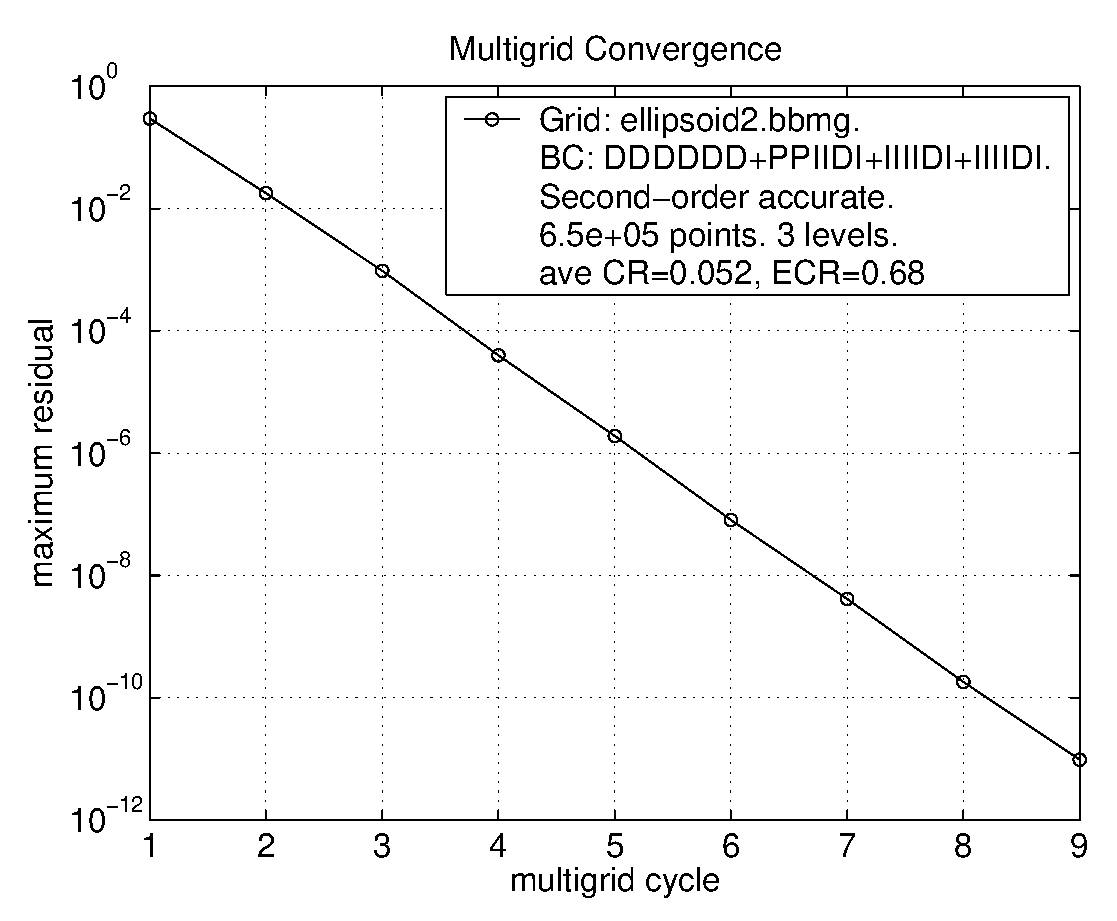
\epsfig{file=residual.ellipsoid2.eps,width=\figWidth}}
% % turn on the grid for placement
% % \psgrid[subgriddiv=2]
% \end{pspicture}
% \end{center}
% \caption{Top: First two levels for an ellipsoid in a box (ellipsoid2.bbmg). 
% Middle left: computed solution. Middle right: error. Bottom: convergence history.
% The multigrid solution of this problem had
% an average convergence rate of CR=.05 per cycle and an effective convergence rate of ECR=.68 per cycle.}
% \label{fig:ellipsoid}
% \end{figure}

\begin{table}[hbt]
\begin{center}
{\tablefontsize
\begin{tabular}{|c|c|c|c|c|} \hline 
 $i$   & $\vert\vert\mbox{res}\vert\vert_\infty$  &  CR     &  WU    & ECR  \\   \hline 
 $ 1$  & $ 1.2e-01$ & $0.020$ & $ 5.0$ & $0.46$ \\ 
 $ 2$  & $ 2.4e-03$ & $0.020$ & $ 5.2$ & $0.47$ \\ 
 $ 3$  & $ 5.3e-05$ & $0.023$ & $ 5.3$ & $0.49$ \\ 
 $ 4$  & $ 1.4e-06$ & $0.026$ & $ 5.6$ & $0.52$ \\ 
 $ 5$  & $ 3.6e-08$ & $0.026$ & $ 5.2$ & $0.50$ \\ 
 $ 6$  & $ 1.0e-09$ & $0.029$ & $ 5.2$ & $0.50$ \\ 
\hline 
\multicolumn{5}{|c|}{Grid: ellipsoid3.bbmg. 03/06/18}  \\
\multicolumn{5}{|c|}{BC: DDDDDD+PPIIDI+IIIIDI+....}  \\
\multicolumn{5}{|c|}{Second-order accurate.}  \\
\multicolumn{5}{|c|}{Trigonometric solution.}  \\
\multicolumn{5}{|c|}{W[2,1]: rb $\omega=1.15$, lz3 $\omega=1.00$}  \\
\multicolumn{5}{|c|}{4.64e+06 grid-points. 4 levels.}  \\
\multicolumn{5}{|c|}{Average CR=$0.024$, ECR=$0.49$.}  \\
\multicolumn{5}{|c|}{time/cycle = 1.32e+01 s.}  \\
\hline 
\end{tabular}
\begin{tabular}{|c|c|c|c|c|} \hline 
 $i$   & $\vert\vert\mbox{res}\vert\vert_\infty$  &  CR     &  WU    & ECR  \\   \hline 
 $ 1$  & $ 1.5e-01$ & $0.020$ & $ 5.1$ & $0.47$ \\ 
 $ 2$  & $ 2.5e-03$ & $0.017$ & $ 5.3$ & $0.46$ \\ 
 $ 3$  & $ 6.1e-05$ & $0.024$ & $ 5.7$ & $0.52$ \\ 
 $ 4$  & $ 8.7e-07$ & $0.014$ & $ 6.0$ & $0.49$ \\ 
 $ 5$  & $ 2.1e-08$ & $0.025$ & $ 5.7$ & $0.52$ \\ 
 $ 6$  & $ 8.5e-10$ & $0.040$ & $ 5.3$ & $0.54$ \\ 
\hline 
\multicolumn{5}{|c|}{Grid: ellipsoid2a.bbmg. 03/06/18}  \\
\multicolumn{5}{|c|}{BC: DDDDDD+PPIIDI+IIIIDI+....}  \\
\multicolumn{5}{|c|}{Second-order accurate.}  \\
\multicolumn{5}{|c|}{Trigonometric solution. IBS-2-4-4}  \\
\multicolumn{5}{|c|}{W[2,1]: rb $\omega=1.15$, lz3 $\omega=1.00$}  \\
\multicolumn{5}{|c|}{2.01e+06 grid-points. 4 levels.}  \\
\multicolumn{5}{|c|}{Average CR=$0.022$, ECR=$0.50$.}  \\
\multicolumn{5}{|c|}{time/cycle = 7.04e+00 s.}  \\
\hline 
\end{tabular}
\begin{tabular}{|c|c|c|c|c|} \hline 
 $i$   & $\vert\vert\mbox{res}\vert\vert_\infty$  &  CR     &  WU    & ECR  \\   \hline 
 $ 1$  & $ 8.6e-02$ & $0.014$ & $ 5.2$ & $0.44$ \\ 
 $ 2$  & $ 1.9e-03$ & $0.022$ & $ 5.4$ & $0.49$ \\ 
 $ 3$  & $ 6.3e-05$ & $0.034$ & $ 5.8$ & $0.56$ \\ 
 $ 4$  & $ 2.2e-06$ & $0.035$ & $ 6.2$ & $0.58$ \\ 
 $ 5$  & $ 6.9e-08$ & $0.031$ & $ 6.2$ & $0.57$ \\ 
 $ 6$  & $ 2.3e-09$ & $0.033$ & $ 6.2$ & $0.58$ \\ 
\hline 
\multicolumn{5}{|c|}{Grid: ellipsoid2a.bbmg. 03/06/18}  \\
\multicolumn{5}{|c|}{BC: DDDDDD+PPIIDI+IIIIDI+....}  \\
\multicolumn{5}{|c|}{Second-order accurate.}  \\
\multicolumn{5}{|c|}{Trigonometric solution. IBS+PBS}  \\
\multicolumn{5}{|c|}{W[2,1]: rb $\omega=1.15$, lz3 $\omega=1.00$}  \\
\multicolumn{5}{|c|}{2.01e+06 grid-points. 4 levels.}  \\
\multicolumn{5}{|c|}{Average CR=$0.027$, ECR=$0.54$.}  \\
\multicolumn{5}{|c|}{time/cycle = 7.05e+00 s.}  \\
\hline 
\end{tabular}
\begin{tabular}{|c|c|c|c|c|} \hline 
 $i$   & $\vert\vert\mbox{res}\vert\vert_\infty$  &  CR     &  WU    & ECR  \\   \hline 
 $ 1$  & $ 1.2e-01$ & $0.017$ & $ 5.3$ & $0.47$ \\ 
 $ 2$  & $ 1.8e-03$ & $0.015$ & $ 5.7$ & $0.48$ \\ 
 $ 3$  & $ 2.7e-05$ & $0.015$ & $ 6.0$ & $0.50$ \\ 
 $ 4$  & $ 2.9e-07$ & $0.011$ & $ 5.6$ & $0.44$ \\ 
 $ 5$  & $ 1.0e-08$ & $0.035$ & $ 5.2$ & $0.52$ \\ 
 $ 6$  & $ 1.6e-10$ & $0.016$ & $ 5.3$ & $0.46$ \\ 
\hline 
\multicolumn{5}{|c|}{Grid: ellipsoid2.bbmg. 03/06/18}  \\
\multicolumn{5}{|c|}{BC: DDDDDD+PPIIDI+IIIIDI+....}  \\
\multicolumn{5}{|c|}{Second-order accurate.}  \\
\multicolumn{5}{|c|}{Trigonometric solution.IBS-2-4-4}  \\
\multicolumn{5}{|c|}{W[2,1]: rb $\omega=1.15$, lz3 $\omega=1.00$}  \\
\multicolumn{5}{|c|}{6.53e+05 grid-points. 3 levels.}  \\
\multicolumn{5}{|c|}{Average CR=$0.017$, ECR=$0.48$.}  \\
\multicolumn{5}{|c|}{time/cycle = 2.77e+00 s.}  \\
\hline 
\end{tabular}
\begin{tabular}{|c|c|c|c|c|} \hline 
 $i$   & res      & rate    &  WU    & ECR  \\   \hline 
 $ 1$  & $ 1.7e+00$ & $0.051$ & $ 5.8$ & $0.60$ \\ 
 $ 2$  & $ 9.1e-02$ & $0.053$ & $ 6.7$ & $0.65$ \\ 
 $ 3$  & $ 3.4e-03$ & $0.037$ & $ 7.5$ & $0.65$ \\ 
 $ 4$  & $ 1.6e-04$ & $0.048$ & $ 7.7$ & $0.67$ \\ 
 $ 5$  & $ 8.1e-06$ & $0.050$ & $ 8.3$ & $0.70$ \\ 
 $ 6$  & $ 4.7e-07$ & $0.057$ & $ 8.5$ & $0.71$ \\ 
 $ 7$  & $ 2.4e-08$ & $0.052$ & $ 8.7$ & $0.71$ \\ 
% $ 8$  & $ 1.5e-09$ & $0.062$ & $ 8.7$ & $0.73$ \\ 
% $ 9$  & $ 6.7e-11$ & $0.045$ & $ 8.5$ & $0.69$ \\ 
\hline 
\multicolumn{5}{|c|}{Grid: ellipsoid2.bbmg.}  \\
\multicolumn{5}{|c|}{Dirichlet boundary conditions.}  \\
\multicolumn{5}{|c|}{Second-order accurate.}  \\
\multicolumn{5}{|c|}{Constant forcing.}  \\
\multicolumn{5}{|c|}{Smoother rb[2,1] $\omega=1.15$}  \\
\multicolumn{5}{|c|}{6.53e+05 grid-points. 3 levels.}  \\
\multicolumn{5}{|c|}{Average CR=$0.050$, ECR=$0.68$.}  \\
\multicolumn{5}{|c|}{time/cycle = 1.58e+00 s.}  \\
\hline 
\end{tabular}
\begin{tabular}{|c|c|c|c|c|} \hline 
 $i$   & $\vert\vert\mbox{res}\vert\vert_\infty$  &  CR     &  WU    & ECR  \\   \hline 
 $ 1$  & $ 3.3e-01$ & $0.044$ & $ 6.0$ & $0.59$ \\ 
 $ 2$  & $ 8.7e-03$ & $0.026$ & $ 6.0$ & $0.54$ \\ 
 $ 3$  & $ 4.4e-04$ & $0.051$ & $ 6.0$ & $0.61$ \\ 
 $ 4$  & $ 1.8e-05$ & $0.041$ & $ 6.3$ & $0.60$ \\ 
 $ 5$  & $ 7.3e-07$ & $0.041$ & $ 6.0$ & $0.59$ \\ 
 $ 6$  & $ 3.6e-08$ & $0.050$ & $ 6.3$ & $0.62$ \\ 
 $ 7$  & $ 1.2e-09$ & $0.034$ & $ 6.3$ & $0.58$ \\ 
\hline 
\multicolumn{5}{|c|}{Grid: ellipsoid2.bbmg.}  \\
\multicolumn{5}{|c|}{BC: DDDDDD+PPIIDI+IIIIDI+....}  \\
\multicolumn{5}{|c|}{Second-order accurate.}  \\
\multicolumn{5}{|c|}{Trigonometric solution.}  \\
\multicolumn{5}{|c|}{W[2,1]: lz3 $\omega=1.20$}  \\
\multicolumn{5}{|c|}{6.53e+05 grid-points. 3 levels.}  \\
\multicolumn{5}{|c|}{Average CR=$0.040$, ECR=$0.59$.}  \\
\multicolumn{5}{|c|}{time/cycle = 1.88e+00 s.}  \\
\hline 
\end{tabular}
\begin{tabular}{|c|c|c|c|c|} \hline 
 $i$   & $\vert\vert\mbox{res}\vert\vert_\infty$  &  CR     &  WU    & ECR  \\   \hline 
 $ 1$  & $ 9.7e-01$ & $0.035$ & $ 4.8$ & $0.50$ \\ 
 $ 2$  & $ 9.9e-02$ & $0.102$ & $ 4.8$ & $0.62$ \\ 
 $ 3$  & $ 5.5e-03$ & $0.056$ & $ 4.7$ & $0.54$ \\ 
 $ 4$  & $ 4.7e-04$ & $0.085$ & $ 4.7$ & $0.59$ \\ 
 $ 5$  & $ 3.5e-05$ & $0.074$ & $ 4.7$ & $0.57$ \\ 
 $ 6$  & $ 2.8e-06$ & $0.082$ & $ 4.7$ & $0.59$ \\ 
 $ 7$  & $ 2.1e-07$ & $0.075$ & $ 4.7$ & $0.58$ \\ 
 $ 8$  & $ 1.7e-08$ & $0.079$ & $ 4.7$ & $0.58$ \\ 
% $ 9$  & $ 1.3e-09$ & $0.075$ & $ 4.7$ & $0.58$ \\ 
% $10$  & $ 9.8e-11$ & $0.077$ & $ 4.7$ & $0.58$ \\ 
\hline 
\multicolumn{5}{|c|}{Grid: ellipsoid2a.bbmg.}  \\
\multicolumn{5}{|c|}{BC: DDDDDD+PPIIDI+IIIIDI+....}  \\
\multicolumn{5}{|c|}{Second-order accurate.}  \\
\multicolumn{5}{|c|}{Trigonometric solution.}  \\
\multicolumn{5}{|c|}{V[2,1]: rb $\omega=1.15$, lz3 $\omega=1.18$}  \\
\multicolumn{5}{|c|}{2.01e+06 grid-points. 4 levels.}  \\
\multicolumn{5}{|c|}{Average CR=$0.072$, ECR=$0.57$.}  \\
\multicolumn{5}{|c|}{time/cycle = 3.16e+00 s.}  \\
\hline 
\end{tabular}
} % end \tablefontsize
\end{center}
\caption{Multigrid convergence rates for an ellipsoid-in-a-box.}
\label{fig:smoothBox}
\end{table}




% ======================================================================================================
% =================================================================================================
\clearpage
\subsection{Multiple spheres in a box}

Figure~\ref{multiSpheres} shows results for a geometry consisting of a collection of spheres in a box.

{
\newcommand{\figWidth}{8.cm}
\newcommand{\trimfig}[2]{\trimPlotb{#1}{#2}{.0}{.0}{.0}{.0}}
\newcommand{\figWidtha}{7.cm}
\newcommand{\trimfiga}[2]{\trimPlotb{#1}{#2}{.0}{.0}{. }{.0}}
\begin{figure}[hbt]
\begin{center}
\begin{tikzpicture}[scale=1]
  \useasboundingbox (0,.4) rectangle (16.,14);  % set the bounding box (so we have less surrounding white space)
%
  \draw ( 0.0,6.) node[anchor=south west,xshift=-4pt,yshift=+0pt] {\trimfig{fig/multiSphere_u}{\figWidth}};
  \draw ( 8.0,6.) node[anchor=south west,xshift=-4pt,yshift=+0pt] {\trimfig{fig/multiSphere_error}{\figWidth}};
%
%  \draw ( 0.0,0.0) node[anchor=south west,xshift=-4pt,yshift=+0pt] {\trimfig{fig/shapes_bbmg4_error}{\figWidth}};
  \draw ( 7.5,0.0) node[anchor=south west,xshift=-4pt,yshift=+0pt] {\trimfiga{fig/residual_multiSphere3}{\figWidtha}};
%
 % \draw (current bounding box.south west) rectangle (current bounding box.north east);
% grid:
% \draw[step=1cm,gray] (0,0) grid (16,15);
\end{tikzpicture}
\end{center}
\caption{Top: computed solution for spheres in a box (multiSphere3). Middle right: error. Bottom: convergence history.}
\label{fig:multiSpheres}
\end{figure}
}




\begin{table}[hbt]
\begin{center}
{\tablefontsize
\begin{tabular}{|c|c|c|c|c|} \hline 
 $i$   & $\vert\vert\mbox{res}\vert\vert_\infty$  &  CR     &  WU    & ECR  \\   \hline 
 $ 1$  & $ 1.9e+00$ & $0.001$ & $ 8.3$ & $0.41$ \\ 
 $ 2$  & $ 6.2e-02$ & $0.033$ & $ 5.3$ & $0.53$ \\ 
 $ 3$  & $ 1.6e-03$ & $0.026$ & $ 5.3$ & $0.50$ \\ 
 $ 4$  & $ 8.4e-05$ & $0.052$ & $ 5.2$ & $0.57$ \\ 
 $ 5$  & $ 2.5e-06$ & $0.030$ & $ 5.3$ & $0.51$ \\ 
 $ 6$  & $ 1.5e-07$ & $0.060$ & $ 5.1$ & $0.58$ \\ 
 $ 7$  & $ 5.2e-09$ & $0.035$ & $ 6.5$ & $0.60$ \\ 
 $ 8$  & $ 3.2e-10$ & $0.063$ & $ 6.1$ & $0.63$ \\ 
\hline 
\multicolumn{5}{|c|}{Grid: multiSphere3. 03/07/23}  \\
\multicolumn{5}{|c|}{BC: DDDDDD+IIIIDI+IIIIDI+....}  \\
\multicolumn{5}{|c|}{Second-order accurate.}  \\
\multicolumn{5}{|c|}{Trigonometric solution.}  \\
\multicolumn{5}{|c|}{Full Multigrid.}  \\
\multicolumn{5}{|c|}{W[2,1]: rb $\omega=1.21$}  \\
\multicolumn{5}{|c|}{5.35e+06 grid-points. 4 levels.}  \\
\multicolumn{5}{|c|}{Average CR=$0.040$, ECR=$0.56$.}  \\
\multicolumn{5}{|c|}{time/cycle = 2.02e+01 s.}  \\
\hline 
\end{tabular}
\begin{tabular}{|c|c|c|c|c|} \hline 
 $i$   & $\vert\vert\mbox{res}\vert\vert_\infty$  &  CR     &  WU    & ECR  \\   \hline 
 $ 1$  & $ 4.5e+02$ & $0.145$ & $ 5.5$ & $0.71$ \\ 
 $ 2$  & $ 8.3e+00$ & $0.019$ & $ 5.7$ & $0.50$ \\ 
 $ 3$  & $ 1.6e-01$ & $0.019$ & $ 5.7$ & $0.50$ \\ 
 $ 4$  & $ 2.3e-02$ & $0.149$ & $ 4.4$ & $0.65$ \\ 
 $ 5$  & $ 3.2e-03$ & $0.139$ & $ 4.4$ & $0.64$ \\ 
 $ 6$  & $ 5.1e-05$ & $0.016$ & $ 5.7$ & $0.48$ \\ 
 $ 7$  & $ 8.8e-07$ & $0.017$ & $ 5.7$ & $0.49$ \\ 
 $ 8$  & $ 1.3e-07$ & $0.149$ & $ 4.4$ & $0.65$ \\ 
 $ 9$  & $ 1.8e-08$ & $0.136$ & $ 4.5$ & $0.64$ \\ 
 $10$  & $ 2.7e-10$ & $0.015$ & $ 6.7$ & $0.53$ \\ 
\hline 
\multicolumn{5}{|c|}{Grid: multiSphere3. 03/07/22}  \\
\multicolumn{5}{|c|}{BC: DDDDDD+IIIIDI+IIIIDI+....}  \\
\multicolumn{5}{|c|}{Second-order accurate.}  \\
\multicolumn{5}{|c|}{Trigonometric solution.}  \\
\multicolumn{5}{|c|}{W[1,1]: rb $\omega=1.13$, lz3 $\omega=1.09$}  \\
\multicolumn{5}{|c|}{5.35e+06 grid-points. 4 levels.}  \\
\multicolumn{5}{|c|}{Average CR=$0.044$, ECR=$0.55$.}  \\
\multicolumn{5}{|c|}{time/cycle = 1.54e+01 s.}  \\
\hline 
\end{tabular}
\begin{tabular}{|c|c|c|c|c|} \hline 
 $i$   & $\vert\vert\mbox{res}\vert\vert_\infty$  &  CR     &  WU    & ECR  \\   \hline 
 $ 1$  & $ 4.1e+01$ & $0.013$ & $ 7.4$ & $0.56$ \\ 
 $ 2$  & $ 1.9e+00$ & $0.046$ & $ 5.3$ & $0.56$ \\ 
 $ 3$  & $ 6.9e-02$ & $0.036$ & $ 6.7$ & $0.61$ \\ 
 $ 4$  & $ 1.1e-04$ & $0.002$ & $ 8.8$ & $0.48$ \\ 
 $ 5$  & $ 4.7e-06$ & $0.042$ & $10.1$ & $0.73$ \\ 
 $ 6$  & $ 1.5e-07$ & $0.033$ & $11.0$ & $0.73$ \\ 
 $ 7$  & $ 2.0e-09$ & $0.013$ & $11.3$ & $0.68$ \\ 
\hline 
\multicolumn{5}{|c|}{Grid: multiSphere3. 03/07/22}  \\
\multicolumn{5}{|c|}{BC: DDDDDD+IIIIDI+IIIIDI+....}  \\
\multicolumn{5}{|c|}{Second-order accurate.}  \\
\multicolumn{5}{|c|}{Trigonometric solution.}  \\
\multicolumn{5}{|c|}{W[2,1]: rb $\omega=1.12$, alz $\omega=1.09$}  \\
\multicolumn{5}{|c|}{5.35e+06 grid-points. 4 levels.}  \\
\multicolumn{5}{|c|}{Average CR=$0.019$, ECR=$0.64$.}  \\
\multicolumn{5}{|c|}{time/cycle = 2.42e+01 s.}  \\
\hline 
\end{tabular}
\begin{tabular}{|c|c|c|c|c|} \hline 
 $i$   & $\vert\vert\mbox{res}\vert\vert_\infty$  &  CR     &  WU    & ECR  \\   \hline 
 $ 1$  & $ 5.5e+01$ & $0.018$ & $ 8.4$ & $0.62$ \\ 
 $ 2$  & $ 2.4e-01$ & $0.004$ & $ 7.8$ & $0.50$ \\ 
 $ 3$  & $ 3.8e-03$ & $0.016$ & $ 7.2$ & $0.56$ \\ 
 $ 4$  & $ 1.6e-04$ & $0.043$ & $ 6.3$ & $0.61$ \\ 
 $ 5$  & $ 3.1e-06$ & $0.019$ & $ 8.5$ & $0.63$ \\ 
 $ 6$  & $ 9.3e-08$ & $0.030$ & $10.0$ & $0.70$ \\ 
 $ 7$  & $ 2.0e-09$ & $0.022$ & $11.2$ & $0.71$ \\ 
\hline 
\multicolumn{5}{|c|}{Grid: multiSphere3. 03/07/22}  \\
\multicolumn{5}{|c|}{BC: DDDDDD+IIIIDI+IIIIDI+....}  \\
\multicolumn{5}{|c|}{Second-order accurate.}  \\
\multicolumn{5}{|c|}{Trigonometric solution.}  \\
\multicolumn{5}{|c|}{W[2,1]: rb $\omega=1.12$, lz3 $\omega=1.09$}  \\
\multicolumn{5}{|c|}{5.35e+06 grid-points. 4 levels.}  \\
\multicolumn{5}{|c|}{Average CR=$0.018$, ECR=$0.63$.}  \\
\multicolumn{5}{|c|}{time/cycle = 2.71e+01 s.}  \\
\hline 
\end{tabular}
\begin{tabular}{|c|c|c|c|c|} \hline 
 $i$   & $\vert\vert\mbox{res}\vert\vert_\infty$  &  CR     &  WU    & ECR  \\   \hline 
 $ 1$  & $ 4.1e+01$ & $0.013$ & $ 8.4$ & $0.60$ \\ 
 $ 2$  & $ 2.5e-01$ & $0.006$ & $ 7.2$ & $0.49$ \\ 
 $ 3$  & $ 9.2e-03$ & $0.037$ & $ 6.3$ & $0.59$ \\ 
 $ 4$  & $ 1.4e-04$ & $0.016$ & $ 8.5$ & $0.61$ \\ 
 $ 5$  & $ 2.1e-06$ & $0.014$ & $10.4$ & $0.66$ \\ 
 $ 6$  & $ 6.6e-08$ & $0.032$ & $ 9.6$ & $0.70$ \\ 
 $ 7$  & $ 1.7e-09$ & $0.026$ & $10.1$ & $0.70$ \\ 
\hline 
\multicolumn{5}{|c|}{Grid: multiSphere3. 03/07/22}  \\
\multicolumn{5}{|c|}{BC: DDDDDD+IIIIDI+IIIIDI+....}  \\
\multicolumn{5}{|c|}{Second-order accurate.}  \\
\multicolumn{5}{|c|}{Trigonometric solution.}  \\
\multicolumn{5}{|c|}{W[2,1]: rb $\omega=1.12$, lz3 $\omega=1.12$}  \\
\multicolumn{5}{|c|}{5.35e+06 grid-points. 4 levels.}  \\
\multicolumn{5}{|c|}{Average CR=$0.019$, ECR=$0.63$.}  \\
\multicolumn{5}{|c|}{time/cycle = 2.53e+01 s.}  \\
\hline 
\end{tabular}
\begin{tabular}{|c|c|c|c|c|} \hline 
 $i$   & $\vert\vert\mbox{res}\vert\vert_\infty$  &  CR     &  WU    & ECR  \\   \hline 
 $ 1$  & $ 8.8e+01$ & $0.029$ & $ 8.4$ & $0.65$ \\ 
 $ 2$  & $ 5.9e-01$ & $0.007$ & $ 8.2$ & $0.54$ \\ 
 $ 3$  & $ 6.4e-03$ & $0.011$ & $ 8.1$ & $0.57$ \\ 
 $ 4$  & $ 1.3e-04$ & $0.021$ & $ 8.4$ & $0.63$ \\ 
 $ 5$  & $ 4.3e-06$ & $0.032$ & $ 9.2$ & $0.69$ \\ 
 $ 6$  & $ 1.4e-07$ & $0.032$ & $10.6$ & $0.72$ \\ 
 $ 7$  & $ 4.4e-09$ & $0.032$ & $11.9$ & $0.75$ \\ 
 $ 8$  & $ 1.4e-10$ & $0.032$ & $11.9$ & $0.75$ \\ 
\hline 
\multicolumn{5}{|c|}{Grid: multiSphere3. 03/07/22}  \\
\multicolumn{5}{|c|}{BC: DDDDDD+IIIIDI+IIIIDI+....}  \\
\multicolumn{5}{|c|}{Second-order accurate.}  \\
\multicolumn{5}{|c|}{Trigonometric solution.}  \\
\multicolumn{5}{|c|}{W[2,1]: rb $\omega=1.12$, lz3 $\omega=1.00$}  \\
\multicolumn{5}{|c|}{5.35e+06 grid-points. 4 levels.}  \\
\multicolumn{5}{|c|}{Average CR=$0.021$, ECR=$0.67$.}  \\
\multicolumn{5}{|c|}{time/cycle = 2.95e+01 s.}  \\
\hline 
\end{tabular}
\begin{tabular}{|c|c|c|c|c|} \hline 
 $i$   & $\vert\vert\mbox{res}\vert\vert_\infty$  &  CR     &  WU    & ECR  \\   \hline 
 $ 1$  & $ 6.5e-01$ & $0.014$ & $ 7.2$ & $0.55$ \\ 
 $ 2$  & $ 9.6e-03$ & $0.015$ & $ 9.1$ & $0.63$ \\ 
 $ 3$  & $ 1.1e-04$ & $0.012$ & $ 8.1$ & $0.58$ \\ 
 $ 4$  & $ 2.8e-06$ & $0.025$ & $ 9.1$ & $0.67$ \\ 
 $ 5$  & $ 1.4e-07$ & $0.049$ & $10.9$ & $0.76$ \\ 
 $ 6$  & $ 2.0e-09$ & $0.014$ & $10.6$ & $0.67$ \\ 
\hline 
\multicolumn{5}{|c|}{Grid: multiSphere3. 03/06/19}  \\
\multicolumn{5}{|c|}{BC: DDDDDD+IIIIDI+IIIIDI+....}  \\
\multicolumn{5}{|c|}{Second-order accurate.}  \\
\multicolumn{5}{|c|}{Trigonometric solution.}  \\
\multicolumn{5}{|c|}{F[2,1]: rb $\omega=1.15$, alz $\omega=1.00$}  \\
\multicolumn{5}{|c|}{5.35e+06 grid-points. 4 levels.}  \\
\multicolumn{5}{|c|}{Average CR=$0.019$, ECR=$0.65$.}  \\
\multicolumn{5}{|c|}{time/cycle = 3.63e+01 s.}  \\
\hline 
\end{tabular}
\begin{tabular}{|c|c|c|c|c|} \hline 
 $i$   & $\vert\vert\mbox{res}\vert\vert_\infty$  &  CR     &  WU    & ECR  \\   \hline 
 $ 1$  & $ 1.7e+00$ & $0.058$ & $ 5.3$ & $0.59$ \\ 
 $ 2$  & $ 5.1e-02$ & $0.031$ & $ 5.1$ & $0.50$ \\ 
 $ 3$  & $ 3.0e-03$ & $0.059$ & $ 5.1$ & $0.58$ \\ 
 $ 4$  & $ 1.0e-04$ & $0.033$ & $ 5.2$ & $0.52$ \\ 
 $ 5$  & $ 6.2e-06$ & $0.061$ & $ 5.3$ & $0.59$ \\ 
 $ 6$  & $ 2.1e-07$ & $0.035$ & $ 5.2$ & $0.52$ \\ 
 $ 7$  & $ 1.3e-08$ & $0.062$ & $ 5.2$ & $0.58$ \\ 
\hline 
\multicolumn{5}{|c|}{Grid: multiSphere3. 03/06/19}  \\
\multicolumn{5}{|c|}{BC: DDDDDD+IIIIDI+IIIIDI+....}  \\
\multicolumn{5}{|c|}{Second-order accurate.}  \\
\multicolumn{5}{|c|}{Trigonometric solution.}  \\
\multicolumn{5}{|c|}{F[2,1]: rb $\omega=1.21$}  \\
\multicolumn{5}{|c|}{5.35e+06 grid-points. 4 levels.}  \\
\multicolumn{5}{|c|}{Average CR=$0.046$, ECR=$0.55$.}  \\
\multicolumn{5}{|c|}{time/cycle = 2.77e+01 s.}  \\
\hline 
\end{tabular}
\begin{tabular}{|c|c|c|c|c|} \hline 
 $i$   & $\vert\vert\mbox{res}\vert\vert_\infty$  &  CR     &  WU    & ECR  \\   \hline 
 $ 1$  & $ 8.0e-01$ & $0.008$ & $ 8.1$ & $0.55$ \\ 
 $ 2$  & $ 9.2e-03$ & $0.011$ & $ 8.1$ & $0.58$ \\ 
 $ 3$  & $ 1.4e-04$ & $0.015$ & $ 7.8$ & $0.59$ \\ 
 $ 4$  & $ 3.2e-06$ & $0.023$ & $ 7.9$ & $0.62$ \\ 
 $ 5$  & $ 7.0e-08$ & $0.022$ & $ 8.5$ & $0.64$ \\ 
 $ 6$  & $ 3.2e-09$ & $0.046$ & $ 9.5$ & $0.72$ \\ 
\hline 
\multicolumn{5}{|c|}{Grid: multiSphere3. 03/06/19}  \\
\multicolumn{5}{|c|}{BC: DDDDDD+IIIIDI+IIIIDI+....}  \\
\multicolumn{5}{|c|}{Second-order accurate.}  \\
\multicolumn{5}{|c|}{Trigonometric solution. IBS-2-4-3}  \\
\multicolumn{5}{|c|}{F[2,1]: rb $\omega=1.15$, lz3 $\omega=1.00$}  \\
\multicolumn{5}{|c|}{5.35e+06 grid-points. 4 levels.}  \\
\multicolumn{5}{|c|}{Average CR=$0.018$, ECR=$0.62$.}  \\
\multicolumn{5}{|c|}{time/cycle = 3.61e+01 s.}  \\
\hline 
\end{tabular}
\begin{tabular}{|c|c|c|c|c|} \hline 
 $i$   & $\vert\vert\mbox{res}\vert\vert_\infty$  &  CR     &  WU    & ECR  \\   \hline 
 $ 1$  & $ 3.4e-01$ & $0.039$ & $ 5.7$ & $0.56$ \\ 
 $ 2$  & $ 4.5e-03$ & $0.013$ & $ 7.3$ & $0.55$ \\ 
 $ 3$  & $ 1.5e-04$ & $0.033$ & $10.0$ & $0.71$ \\ 
 $ 4$  & $ 3.5e-06$ & $0.023$ & $11.0$ & $0.71$ \\ 
 $ 5$  & $ 1.1e-07$ & $0.030$ & $11.0$ & $0.73$ \\ 
 $ 6$  & $ 2.8e-09$ & $0.026$ & $11.0$ & $0.72$ \\ 
\hline 
\multicolumn{5}{|c|}{Grid: multiSphere3. 03/06/19}  \\
\multicolumn{5}{|c|}{BC: DDDDDD+IIIIDI+IIIIDI+....}  \\
\multicolumn{5}{|c|}{Second-order accurate.}  \\
\multicolumn{5}{|c|}{Trigonometric solution.}  \\
\multicolumn{5}{|c|}{W[2,1]: rb $\omega=1.15$, lz3 $\omega=1.00$}  \\
\multicolumn{5}{|c|}{5.35e+06 grid-points. 4 levels.}  \\
\multicolumn{5}{|c|}{Average CR=$0.026$, ECR=$0.68$.}  \\
\multicolumn{5}{|c|}{time/cycle = 4.49e+01 s.}  \\
\hline 
\end{tabular}
\begin{tabular}{|c|c|c|c|c|} \hline 
 $i$   & $\vert\vert\mbox{res}\vert\vert_\infty$  &  CR     &  WU    & ECR  \\   \hline 
 $ 1$  & $ 1.7e+00$ & $0.039$ & $ 6.1$ & $0.59$ \\ 
 $ 2$  & $ 4.5e-02$ & $0.027$ & $ 6.8$ & $0.59$ \\ 
 $ 3$  & $ 2.7e-03$ & $0.059$ & $ 6.4$ & $0.64$ \\ 
 $ 4$  & $ 5.6e-05$ & $0.021$ & $ 7.0$ & $0.58$ \\ 
 $ 5$  & $ 1.5e-06$ & $0.028$ & $ 8.8$ & $0.66$ \\ 
 $ 6$  & $ 8.3e-08$ & $0.054$ & $ 6.7$ & $0.65$ \\ 
 $ 7$  & $ 1.8e-09$ & $0.022$ & $ 7.2$ & $0.59$ \\ 
\hline 
\multicolumn{5}{|c|}{Grid: multiSphere3.}  \\
\multicolumn{5}{|c|}{BC: DDDDDD+IIIIDI+IIIIDI+....}  \\
\multicolumn{5}{|c|}{Second-order accurate.}  \\
\multicolumn{5}{|c|}{Trigonometric solution.}  \\
\multicolumn{5}{|c|}{W[2,1]: alz $\omega=1.20$ (SPLIT)}  \\
\multicolumn{5}{|c|}{5.35e+06 grid-points. 4 levels.}  \\
\multicolumn{5}{|c|}{Average CR=$0.033$, ECR=$0.61$.}  \\
\multicolumn{5}{|c|}{time/cycle = 2.51e+01 s.}  \\
\hline 
\end{tabular}
\begin{tabular}{|c|c|c|c|c|} \hline 
 $i$   & $\vert\vert\mbox{res}\vert\vert_\infty$  &  CR     &  WU    & ECR  \\   \hline 
 $ 1$  & $ 1.8e+00$ & $0.041$ & $ 6.0$ & $0.58$ \\ 
 $ 2$  & $ 3.1e-02$ & $0.017$ & $ 7.9$ & $0.60$ \\ 
 $ 3$  & $ 1.4e-03$ & $0.044$ & $ 7.7$ & $0.66$ \\ 
 $ 4$  & $ 5.5e-05$ & $0.041$ & $ 7.4$ & $0.65$ \\ 
 $ 5$  & $ 1.8e-06$ & $0.033$ & $ 9.2$ & $0.69$ \\ 
 $ 6$  & $ 4.6e-08$ & $0.025$ & $10.9$ & $0.71$ \\ 
 $ 7$  & $ 1.6e-09$ & $0.034$ & $11.2$ & $0.74$ \\ 
\hline 
\multicolumn{5}{|c|}{Grid: multiSphere3.}  \\
\multicolumn{5}{|c|}{BC: DDDDDD+IIIIDI+IIIIDI+....}  \\
\multicolumn{5}{|c|}{Second-order accurate.}  \\
\multicolumn{5}{|c|}{Trigonometric solution.}  \\
\multicolumn{5}{|c|}{W[2,1]: lz3 $\omega=1.20$}  \\
\multicolumn{5}{|c|}{5.35e+06 grid-points. 4 levels.}  \\
\multicolumn{5}{|c|}{Average CR=$0.032$, ECR=$0.67$.}  \\
\multicolumn{5}{|c|}{time/cycle = 2.93e+01 s.}  \\
\hline 
\end{tabular}
} % end \tablefontsize
\end{center}
\caption{Multigrid convergence rates for spheres in a box.}
\label{fig:multiSphereI}
\end{table}



\begin{table}[hbt]
\begin{center}
{\tablefontsize
\begin{tabular}{|c|c|c|c|c|} \hline 
 $i$   & $\vert\vert\mbox{res}\vert\vert_\infty$  &  CR     &  WU    & ECR  \\   \hline 
 $ 1$  & $ 3.8e+00$ & $0.051$ & $ 8.4$ & $0.70$ \\ 
 $ 2$  & $ 7.9e-02$ & $0.021$ & $ 9.9$ & $0.68$ \\ 
 $ 3$  & $ 4.0e-03$ & $0.051$ & $ 9.5$ & $0.73$ \\ 
 $ 4$  & $ 3.1e-04$ & $0.076$ & $ 9.5$ & $0.76$ \\ 
 $ 5$  & $ 3.3e-05$ & $0.109$ & $ 9.6$ & $0.79$ \\ 
 $ 6$  & $ 3.6e-06$ & $0.108$ & $ 9.7$ & $0.80$ \\ 
 $ 7$  & $ 3.1e-07$ & $0.085$ & $ 9.7$ & $0.78$ \\ 
 $ 8$  & $ 3.2e-08$ & $0.103$ & $ 9.6$ & $0.79$ \\ 
 $ 9$  & $ 3.3e-09$ & $0.105$ & $ 9.5$ & $0.79$ \\ 
\hline 
\multicolumn{5}{|c|}{Grid: multiSphere3.}  \\
\multicolumn{5}{|c|}{BC: DDDDDD+IIIIDI+IIIIDI+....}  \\
\multicolumn{5}{|c|}{Second-order accurate.}  \\
\multicolumn{5}{|c|}{Trigonometric solution.}  \\
\multicolumn{5}{|c|}{V[2,1]: rb $\omega=1.15$, alz $\omega=1.00$}  \\
\multicolumn{5}{|c|}{5.35e+06 grid-points. 4 levels.}  \\
\multicolumn{5}{|c|}{Average CR=$0.071$, ECR=$0.76$.}  \\
\multicolumn{5}{|c|}{time/cycle = 2.28e+01 s.}  \\
\hline 
\end{tabular}
\begin{tabular}{|c|c|c|c|c|} \hline 
 $i$   & $\vert\vert\mbox{res}\vert\vert_\infty$  &  CR     &  WU    & ECR  \\   \hline 
 $ 1$  & $ 1.7e+00$ & $0.029$ & $ 6.4$ & $0.57$ \\ 
 $ 2$  & $ 1.2e-01$ & $0.072$ & $ 6.4$ & $0.66$ \\ 
 $ 3$  & $ 1.5e-02$ & $0.122$ & $ 6.4$ & $0.72$ \\ 
 $ 4$  & $ 2.0e-03$ & $0.134$ & $ 6.4$ & $0.73$ \\ 
 $ 5$  & $ 2.7e-04$ & $0.132$ & $ 6.4$ & $0.73$ \\ 
 $ 6$  & $ 3.6e-05$ & $0.133$ & $ 6.4$ & $0.73$ \\ 
 $ 7$  & $ 4.7e-06$ & $0.132$ & $ 6.4$ & $0.73$ \\ 
 $ 8$  & $ 6.2e-07$ & $0.132$ & $ 6.4$ & $0.73$ \\ 
 $ 9$  & $ 8.2e-08$ & $0.133$ & $ 6.4$ & $0.73$ \\ 
\hline 
\multicolumn{5}{|c|}{Grid: multiSphere3.}  \\
\multicolumn{5}{|c|}{BC: DDDDDD+IIIIDI+IIIIDI+....}  \\
\multicolumn{5}{|c|}{Second-order accurate.}  \\
\multicolumn{5}{|c|}{Trigonometric solution.}  \\
\multicolumn{5}{|c|}{V[2,1]: rb $\omega=1.15$}  \\
\multicolumn{5}{|c|}{5.35e+06 grid-points. 4 levels.}  \\
\multicolumn{5}{|c|}{Average CR=$0.104$, ECR=$0.70$.}  \\
\multicolumn{5}{|c|}{time/cycle = 1.42e+01 s.}  \\
\hline 
\end{tabular}
\begin{tabular}{|c|c|c|c|c|} \hline 
 $i$   & $\vert\vert\mbox{res}\vert\vert_\infty$  &  CR     &  WU    & ECR  \\   \hline 
 $ 1$  & $ 1.4e+00$ & $0.024$ & $ 6.7$ & $0.57$ \\ 
 $ 2$  & $ 5.2e-02$ & $0.038$ & $ 6.7$ & $0.61$ \\ 
 $ 3$  & $ 2.6e-03$ & $0.051$ & $ 6.7$ & $0.64$ \\ 
 $ 4$  & $ 3.8e-04$ & $0.145$ & $ 6.7$ & $0.75$ \\ 
 $ 5$  & $ 5.5e-05$ & $0.143$ & $ 6.7$ & $0.75$ \\ 
 $ 6$  & $ 7.6e-06$ & $0.138$ & $ 6.7$ & $0.74$ \\ 
 $ 7$  & $ 1.0e-06$ & $0.135$ & $ 6.7$ & $0.74$ \\ 
 $ 8$  & $ 1.4e-07$ & $0.134$ & $ 6.7$ & $0.74$ \\ 
 $ 9$  & $ 1.8e-08$ & $0.134$ & $ 6.7$ & $0.74$ \\ 
\hline 
\multicolumn{5}{|c|}{Grid: multiSphere3.}  \\
\multicolumn{5}{|c|}{BC: DDDDDD+IIIIDI+IIIIDI+....}  \\
\multicolumn{5}{|c|}{Second-order accurate.}  \\
\multicolumn{5}{|c|}{Trigonometric solution.}  \\
\multicolumn{5}{|c|}{W[2,1]: rb $\omega=1.15$}  \\
\multicolumn{5}{|c|}{5.35e+06 grid-points. 4 levels.}  \\
\multicolumn{5}{|c|}{Average CR=$0.088$, ECR=$0.70$.}  \\
\multicolumn{5}{|c|}{time/cycle = 1.93e+01 s.}  \\
\hline 
\end{tabular}
\begin{tabular}{|c|c|c|c|c|} \hline 
 $i$   & $\vert\vert\mbox{res}\vert\vert_\infty$  &  CR     &  WU    & ECR  \\   \hline 
 $ 1$  & $ 5.2e-01$ & $0.013$ & $ 7.9$ & $0.58$ \\ 
 $ 2$  & $ 1.3e-02$ & $0.024$ & $ 8.5$ & $0.64$ \\ 
 $ 3$  & $ 8.2e-04$ & $0.065$ & $ 8.5$ & $0.72$ \\ 
 $ 4$  & $ 7.9e-05$ & $0.096$ & $ 8.4$ & $0.76$ \\ 
 $ 5$  & $ 7.9e-06$ & $0.100$ & $ 8.4$ & $0.76$ \\ 
 $ 6$  & $ 7.8e-07$ & $0.099$ & $ 8.4$ & $0.76$ \\ 
 $ 7$  & $ 7.7e-08$ & $0.098$ & $ 8.4$ & $0.76$ \\ 
 $ 8$  & $ 7.5e-09$ & $0.098$ & $ 8.4$ & $0.76$ \\ 
 $ 9$  & $ 7.3e-10$ & $0.097$ & $ 8.4$ & $0.76$ \\ 
\hline 
\multicolumn{5}{|c|}{Grid: multiSphere3.}  \\
\multicolumn{5}{|c|}{BC: DDDDDD+IIIIDI+IIIIDI+....}  \\
\multicolumn{5}{|c|}{Second-order accurate.}  \\
\multicolumn{5}{|c|}{Trigonometric solution.}  \\
\multicolumn{5}{|c|}{W[2,1]: rb $\omega=1.15$}  \\
\multicolumn{5}{|c|}{5.35e+06 grid-points. 4 levels.}  \\
\multicolumn{5}{|c|}{Average CR=$0.064$, ECR=$0.72$.}  \\
\multicolumn{5}{|c|}{time/cycle = 2.09e+01 s.}  \\
\hline 
\end{tabular}
\begin{tabular}{|c|c|c|c|c|} \hline 
 $i$   & $\vert\vert\mbox{res}\vert\vert_\infty$  &  CR     &  WU    & ECR  \\   \hline 
 $ 1$  & $ 1.0e-01$ & $0.007$ & $21.2$ & $0.79$ \\ 
 $ 2$  & $ 1.8e-03$ & $0.018$ & $21.2$ & $0.83$ \\ 
 $ 3$  & $ 2.3e-05$ & $0.013$ & $22.2$ & $0.82$ \\ 
 $ 4$  & $ 4.5e-07$ & $0.019$ & $23.7$ & $0.85$ \\ 
 $ 5$  & $ 4.5e-09$ & $0.010$ & $24.5$ & $0.83$ \\ 
 $ 6$  & $ 9.5e-11$ & $0.021$ & $23.3$ & $0.85$ \\ 
\hline 
\multicolumn{5}{|c|}{Grid: multiSphere3.}  \\
\multicolumn{5}{|c|}{BC: DDDDDD+IIIIDI+IIIIDI+....}  \\
\multicolumn{5}{|c|}{Second-order accurate.}  \\
\multicolumn{5}{|c|}{Trigonometric solution.}  \\
\multicolumn{5}{|c|}{W[2,1]: alz $\omega=1.20$ (TRUE)}  \\
\multicolumn{5}{|c|}{5.35e+06 grid-points. 4 levels.}  \\
\multicolumn{5}{|c|}{Average CR=$0.014$, ECR=$0.83$.}  \\
\multicolumn{5}{|c|}{time/cycle = 6.35e+01 s.}  \\
\hline 
\end{tabular}
\begin{tabular}{|c|c|c|c|c|} \hline 
 $i$   & $\vert\vert\mbox{res}\vert\vert_\infty$  &  CR     &  WU    & ECR  \\   \hline 
 $ 1$  & $ 1.7e+00$ & $0.039$ & $ 6.1$ & $0.59$ \\ 
 $ 2$  & $ 4.5e-02$ & $0.027$ & $ 6.8$ & $0.59$ \\ 
 $ 3$  & $ 2.7e-03$ & $0.059$ & $ 6.4$ & $0.64$ \\ 
 $ 4$  & $ 5.6e-05$ & $0.021$ & $ 7.0$ & $0.58$ \\ 
 $ 5$  & $ 1.5e-06$ & $0.028$ & $ 8.8$ & $0.66$ \\ 
 $ 6$  & $ 8.3e-08$ & $0.054$ & $ 6.7$ & $0.65$ \\ 
 $ 7$  & $ 1.8e-09$ & $0.022$ & $ 7.2$ & $0.59$ \\ 
\hline 
\multicolumn{5}{|c|}{Grid: multiSphere3.}  \\
\multicolumn{5}{|c|}{BC: DDDDDD+IIIIDI+IIIIDI+....}  \\
\multicolumn{5}{|c|}{Second-order accurate.}  \\
\multicolumn{5}{|c|}{Trigonometric solution.}  \\
\multicolumn{5}{|c|}{W[2,1]: alz $\omega=1.20$ (SPLIT)}  \\
\multicolumn{5}{|c|}{5.35e+06 grid-points. 4 levels.}  \\
\multicolumn{5}{|c|}{Average CR=$0.033$, ECR=$0.61$.}  \\
\multicolumn{5}{|c|}{time/cycle = 2.51e+01 s.}  \\
\hline 
\end{tabular}
\begin{tabular}{|c|c|c|c|c|} \hline 
 $i$   & $\vert\vert\mbox{res}\vert\vert_\infty$  &  CR     &  WU    & ECR  \\   \hline 
 $ 1$  & $ 1.8e+00$ & $0.041$ & $ 6.0$ & $0.58$ \\ 
 $ 2$  & $ 3.1e-02$ & $0.017$ & $ 7.9$ & $0.60$ \\ 
 $ 3$  & $ 1.4e-03$ & $0.044$ & $ 7.7$ & $0.66$ \\ 
 $ 4$  & $ 5.5e-05$ & $0.041$ & $ 7.4$ & $0.65$ \\ 
 $ 5$  & $ 1.8e-06$ & $0.033$ & $ 9.2$ & $0.69$ \\ 
 $ 6$  & $ 4.6e-08$ & $0.025$ & $10.9$ & $0.71$ \\ 
 $ 7$  & $ 1.6e-09$ & $0.034$ & $11.2$ & $0.74$ \\ 
\hline 
\multicolumn{5}{|c|}{Grid: multiSphere3.}  \\
\multicolumn{5}{|c|}{BC: DDDDDD+IIIIDI+IIIIDI+....}  \\
\multicolumn{5}{|c|}{Second-order accurate.}  \\
\multicolumn{5}{|c|}{Trigonometric solution.}  \\
\multicolumn{5}{|c|}{W[2,1]: lz3 $\omega=1.20$}  \\
\multicolumn{5}{|c|}{5.35e+06 grid-points. 4 levels.}  \\
\multicolumn{5}{|c|}{Average CR=$0.032$, ECR=$0.67$.}  \\
\multicolumn{5}{|c|}{time/cycle = 2.93e+01 s.}  \\
\hline 
\end{tabular}
} % end \tablefontsize
\end{center}
\caption{Multigrid convergence rates for spheres in a box.}
\label{fig:multiSphereII}
\end{table}






% =================================================================================================
\clearpage
\subsection{Sub-in-a-Box}

  The sub in a box grid is shown figure~\ref{fig:sub}. Also shown are the computed
solution and error.

{
\newcommand{\figWidth}{10cm}
\newcommand{\trimfig}[2]{\trimPlotb{#1}{#2}{.0}{.0}{.2}{.2}}
\newcommand{\figWidtha}{7.cm}
\newcommand{\trimfiga}[2]{\trimPlotb{#1}{#2}{.0}{.0}{. }{.0}}
\begin{figure}[hbt]
\begin{center}
\begin{tikzpicture}[scale=1]
  \useasboundingbox (0,.5) rectangle (17.5,12.5);  % set the bounding box (so we have less surrounding white space)
%
  \draw ( 0.0,6.5 ) node[anchor=south west,xshift=-4pt,yshift=+0pt] {\trimfig{fig/subAndFins_u}{\figWidth}};
  \draw ( 0.0,0.0 ) node[anchor=south west,xshift=-4pt,yshift=+0pt] {\trimfig{fig/subAndFins_error}{\figWidth}};
%
%  \draw ( 0.0,0.0) node[anchor=south west,xshift=-4pt,yshift=+0pt] {\trimfig{fig/shapes_bbmg4_error}{\figWidth}};
  \draw (10.5,0.0) node[anchor=south west,xshift=-4pt,yshift=+0pt] {\trimfiga{fig/residual_subAndFins}{\figWidtha}};
%
 % \draw (current bounding box.south west) rectangle (current bounding box.north east);
% grid:
% \draw[step=1cm,gray] (0,0) grid (17,12.5);
\end{tikzpicture}
\end{center}
\caption{Top: First two levels for an sub in a box (subAndFins). 
Top left: computed solution. Bottom left: error. Right: convergence history.}
\label{fig:sub}
\end{figure}
}



%- %
%- \renewcommand{\figWidth}{.8\linewidth}
%- \renewcommand{\figWidthb}{.5\linewidth}
%- \renewcommand{\clipfig}[1]{\psclip{\psframe[linewidth=2pt](-.5,3.0)(15,11.25)}\epsfig{#1}\endpsclip}
%- \begin{figure}
%- \begin{center}
%- \begin{pspicture}(0,.0)(16.5,19.5)
%- \rput(8.5 ,16.75){\clipfig{file=subAndSail.u.ps,width=\figWidth}}
%- \rput(8.5 , 8.5){\clipfig{file=subAndSail.error.ps,width=\figWidth}}
%- \rput(9.0, 3.0){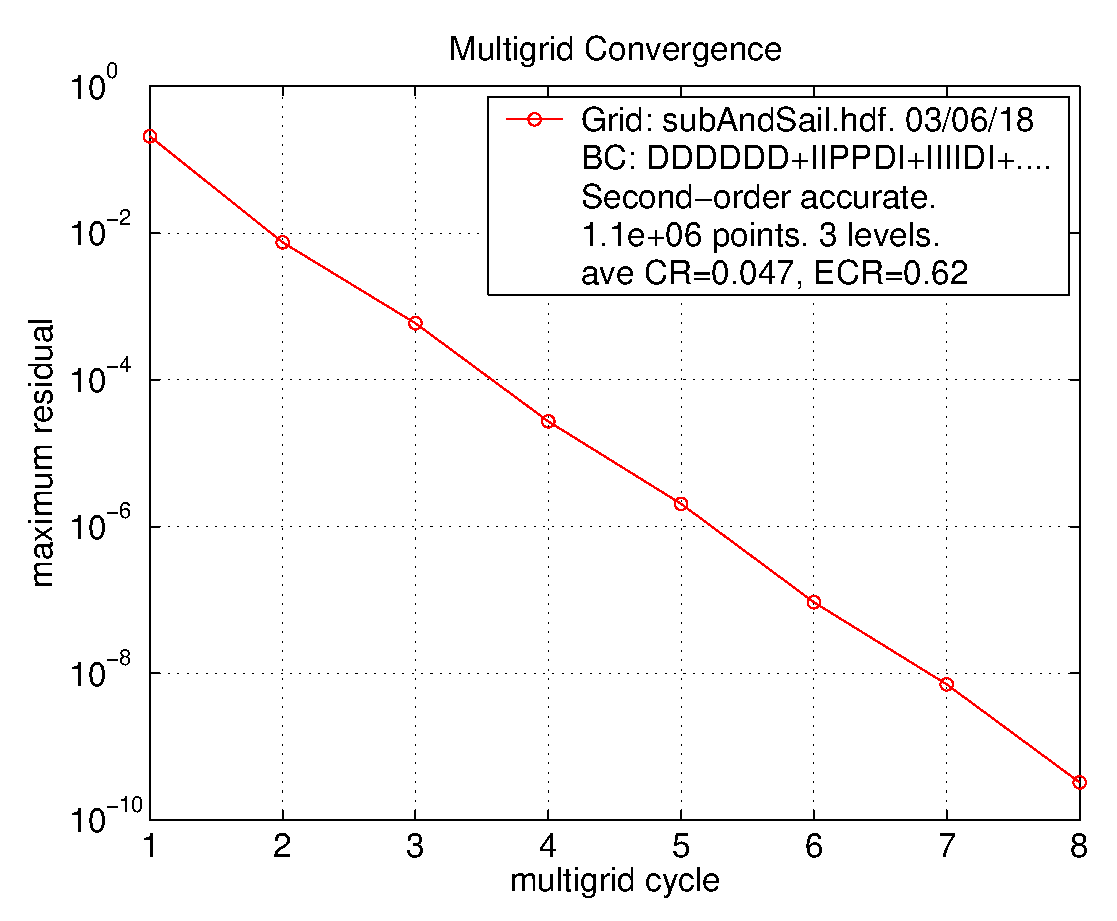
\epsfig{file=residual.subAndSail.eps,width=\figWidthb}}
%- % turn on the grid for placement
%- % \psgrid[subgriddiv=2]
%- \end{pspicture}
%- \end{center}
%- \caption{Top: First two levels for an sub in a box (subAndSail). 
%- Middle left: computed solution. Middle right: error. Bottom: convergence history.}
%- \label{fig:sub}
%- \end{figure}
%- 
%- \begin{figure}
%- \begin{center}
%- \begin{pspicture}(0,.0)(16.5,19.5)
%- \rput(8.5 ,16.75){\clipfig{file=\ogmgDir/subAndFins.u.ps,width=\figWidth}}
%- \rput(8.5 , 8.5){\clipfig{file=\ogmgDir/subAndFins.error.ps,width=\figWidth}}
%- \rput(9.0, 3.0){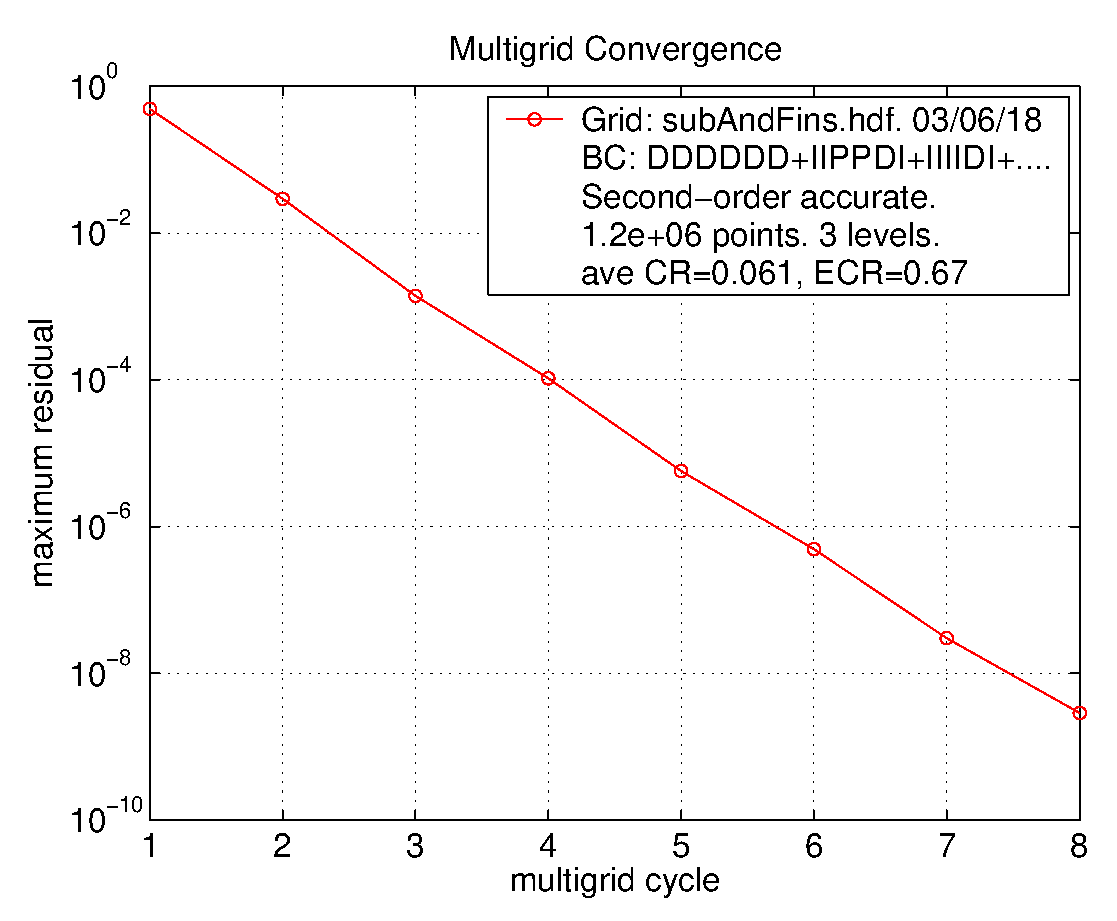
\epsfig{file=\ogmgDir/residual.subAndFins.eps,width=\figWidthb}}
%- % turn on the grid for placement
%- % \psgrid[subgriddiv=2]
%- \end{pspicture}
%- \end{center}
%- \caption{Top: First two levels for an sub in a box (subAndFins). 
%- Middle left: computed solution. Middle right: error. Bottom: convergence history.}
%- \label{fig:sub}
%- \end{figure}

% \renewcommand{\figWidth}{.5\linewidth}
% \renewcommand{\clipfig}[1]{\psclip{\psframe[linecolor=white](.1,.7)(8.9,7.7)}\epsfig{#1}\endpsclip}
% \begin{figure}
% \begin{center}
% \begin{pspicture}(0,-5.)(16.5,13.2)
% % \rput(3.9 ,10.6){\clipfig{file=ellipsoid0.ps,width=\figWidth}}
% % \rput(12.8,10.6){\clipfig{file=ellipsoid1.ps,width=\figWidth}}
% \rput(3.9 , 4.5){\clipfig{file=subAndSail.u.ps,width=\figWidth}}
% \rput(12.8, 4.5){\clipfig{file=subAndSail.error.ps,width=\figWidth}}
% \rput(8.,-2.2){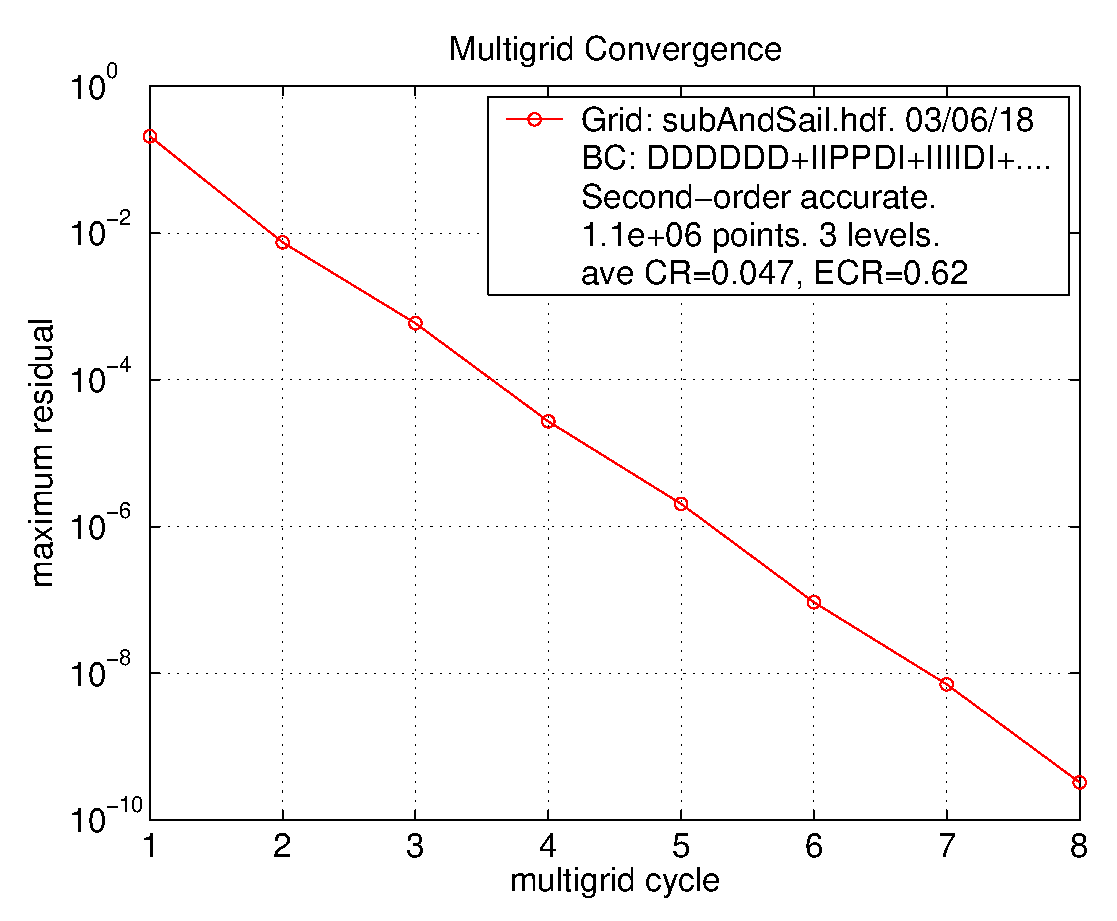
\epsfig{file=residual.subAndSail.eps,width=\figWidth}}
% % turn on the grid for placement
% % \psgrid[subgriddiv=2]
% \end{pspicture}
% \end{center}
% \caption{Top: First two levels for an sub in a box (subAndSail). 
% Middle left: computed solution. Middle right: error. Bottom: convergence history.}
% \label{fig:sub}
% \end{figure}

\begin{table}[hbt]
\begin{center}
{\tablefontsize
\begin{tabular}{|c|c|c|c|c|} \hline 
 $i$   & $\vert\vert\mbox{res}\vert\vert_\infty$  &  CR     &  WU    & ECR  \\   \hline 
 $ 1$  & $ 2.1e-01$ & $0.016$ & $ 5.5$ & $0.47$ \\ 
 $ 2$  & $ 7.5e-03$ & $0.036$ & $ 6.0$ & $0.58$ \\ 
 $ 3$  & $ 5.9e-04$ & $0.079$ & $ 6.4$ & $0.67$ \\ 
 $ 4$  & $ 2.7e-05$ & $0.046$ & $ 6.5$ & $0.62$ \\ 
 $ 5$  & $ 2.0e-06$ & $0.076$ & $ 6.5$ & $0.67$ \\ 
 $ 6$  & $ 9.3e-08$ & $0.045$ & $ 6.6$ & $0.62$ \\ 
 $ 7$  & $ 7.1e-09$ & $0.076$ & $ 6.6$ & $0.68$ \\ 
 $ 8$  & $ 3.3e-10$ & $0.046$ & $ 6.6$ & $0.63$ \\ 
\hline 
\multicolumn{5}{|c|}{Grid: subAndSail.hdf. 03/06/18}  \\
\multicolumn{5}{|c|}{BC: DDDDDD+IIPPDI+IIIIDI+....}  \\
\multicolumn{5}{|c|}{Second-order accurate.}  \\
\multicolumn{5}{|c|}{Trigonometric solution.}  \\
\multicolumn{5}{|c|}{W[2,1]: rb $\omega=1.15$, lz3 $\omega=1.00$}  \\
\multicolumn{5}{|c|}{1.11e+06 grid-points. 3 levels.}  \\
\multicolumn{5}{|c|}{Average CR=$0.047$, ECR=$0.62$.}  \\
\multicolumn{5}{|c|}{time/cycle = 6.70e+00 s.}  \\
\hline 
\end{tabular}
\begin{tabular}{|c|c|c|c|c|} \hline 
 $i$   & $\vert\vert\mbox{res}\vert\vert_\infty$  &  CR     &  WU    & ECR  \\   \hline 
 $ 1$  & $ 8.5e-02$ & $0.030$ & $ 5.2$ & $0.51$ \\ 
 $ 2$  & $ 1.6e-03$ & $0.019$ & $ 5.5$ & $0.49$ \\ 
 $ 3$  & $ 5.5e-05$ & $0.034$ & $ 5.8$ & $0.56$ \\ 
 $ 4$  & $ 2.7e-06$ & $0.049$ & $ 5.8$ & $0.60$ \\ 
 $ 5$  & $ 1.5e-07$ & $0.054$ & $ 5.8$ & $0.61$ \\ 
 $ 6$  & $ 8.8e-09$ & $0.061$ & $ 5.9$ & $0.62$ \\ 
 $ 7$  & $ 5.3e-10$ & $0.060$ & $ 5.9$ & $0.62$ \\ 
\hline 
\multicolumn{5}{|c|}{Grid: subHull.hdf. 03/06/18}  \\
\multicolumn{5}{|c|}{BC: DDDDDD+IIPPDI+IIIIDI+....}  \\
\multicolumn{5}{|c|}{Second-order accurate.}  \\
\multicolumn{5}{|c|}{Trigonometric solution.IBS-3-4-4}  \\
\multicolumn{5}{|c|}{W[2,1]: rb $\omega=1.15$, lz3 $\omega=1.00$}  \\
\multicolumn{5}{|c|}{1.37e+06 grid-points. 3 levels.}  \\
\multicolumn{5}{|c|}{Average CR=$0.041$, ECR=$0.57$.}  \\
\multicolumn{5}{|c|}{time/cycle = 6.52e+00 s.}  \\
\hline 
\end{tabular}
\begin{tabular}{|c|c|c|c|c|} \hline 
 $i$   & $\vert\vert\mbox{res}\vert\vert_\infty$  &  CR     &  WU    & ECR  \\   \hline 
 $ 1$  & $ 4.9e-01$ & $0.032$ & $ 6.2$ & $0.57$ \\ 
 $ 2$  & $ 2.9e-02$ & $0.059$ & $ 6.5$ & $0.65$ \\ 
 $ 3$  & $ 1.4e-03$ & $0.048$ & $ 7.0$ & $0.65$ \\ 
 $ 4$  & $ 1.1e-04$ & $0.075$ & $ 7.3$ & $0.70$ \\ 
 $ 5$  & $ 5.7e-06$ & $0.054$ & $ 7.2$ & $0.67$ \\ 
 $ 6$  & $ 4.9e-07$ & $0.086$ & $ 7.1$ & $0.71$ \\ 
 $ 7$  & $ 3.0e-08$ & $0.061$ & $ 7.1$ & $0.67$ \\ 
 $ 8$  & $ 2.9e-09$ & $0.095$ & $ 7.1$ & $0.72$ \\ 
\hline 
\multicolumn{5}{|c|}{Grid: subAndFins.hdf. 03/06/18}  \\
\multicolumn{5}{|c|}{BC: DDDDDD+IIPPDI+IIIIDI+....}  \\
\multicolumn{5}{|c|}{Second-order accurate.}  \\
\multicolumn{5}{|c|}{Trigonometric solution.IBS-2-4-4}  \\
\multicolumn{5}{|c|}{W[2,1]: rb $\omega=1.15$, lz3 $\omega=1.00$}  \\
\multicolumn{5}{|c|}{1.22e+06 grid-points. 3 levels.}  \\
\multicolumn{5}{|c|}{Average CR=$0.061$, ECR=$0.67$.}  \\
\multicolumn{5}{|c|}{time/cycle = 9.23e+00 s.}  \\
\hline 
\end{tabular}
\begin{tabular}{|c|c|c|c|c|} \hline 
 $i$   & $\vert\vert\mbox{res}\vert\vert_\infty$  &  CR     &  WU    & ECR  \\   \hline 
 $ 1$  & $ 8.9e-02$ & $0.032$ & $ 5.2$ & $0.51$ \\ 
 $ 2$  & $ 2.7e-03$ & $0.031$ & $ 5.5$ & $0.53$ \\ 
 $ 3$  & $ 1.5e-04$ & $0.055$ & $ 5.9$ & $0.61$ \\ 
 $ 4$  & $ 9.3e-06$ & $0.062$ & $ 5.9$ & $0.62$ \\ 
 $ 5$  & $ 5.9e-07$ & $0.064$ & $ 5.9$ & $0.63$ \\ 
 $ 6$  & $ 3.9e-08$ & $0.067$ & $ 5.9$ & $0.63$ \\ 
 $ 7$  & $ 2.6e-09$ & $0.066$ & $ 5.9$ & $0.63$ \\ 
 $ 8$  & $ 1.7e-10$ & $0.067$ & $ 5.9$ & $0.63$ \\ 
\hline 
\multicolumn{5}{|c|}{Grid: subHull.hdf. 03/06/18}  \\
\multicolumn{5}{|c|}{BC: DDDDDD+IIPPDI+IIIIDI+....}  \\
\multicolumn{5}{|c|}{Second-order accurate.}  \\
\multicolumn{5}{|c|}{Trigonometric solution. IBS-2-4-4 }  \\
\multicolumn{5}{|c|}{W[2,1]: rb $\omega=1.15$, lz3 $\omega=1.00$}  \\
\multicolumn{5}{|c|}{1.37e+06 grid-points. 3 levels.}  \\
\multicolumn{5}{|c|}{Average CR=$0.053$, ECR=$0.60$.}  \\
\multicolumn{5}{|c|}{time/cycle = 6.08e+00 s.}  \\
\hline 
\end{tabular}
\begin{tabular}{|c|c|c|c|c|} \hline 
 $i$   & $\vert\vert\mbox{res}\vert\vert_\infty$  &  CR     &  WU    & ECR  \\   \hline 
 $ 1$  & $ 1.3e-01$ & $0.044$ & $ 4.9$ & $0.53$ \\ 
 $ 2$  & $ 5.1e-03$ & $0.041$ & $ 5.1$ & $0.54$ \\ 
 $ 3$  & $ 2.8e-04$ & $0.054$ & $ 5.5$ & $0.59$ \\ 
 $ 4$  & $ 1.7e-05$ & $0.061$ & $ 6.2$ & $0.64$ \\ 
 $ 5$  & $ 1.1e-06$ & $0.068$ & $ 7.0$ & $0.68$ \\ 
 $ 6$  & $ 7.9e-08$ & $0.069$ & $ 7.6$ & $0.70$ \\ 
 $ 7$  & $ 6.1e-09$ & $0.077$ & $ 7.6$ & $0.71$ \\ 
 $ 8$  & $ 4.1e-10$ & $0.068$ & $ 7.6$ & $0.70$ \\ 
\hline 
\multicolumn{5}{|c|}{Grid: subHull.hdf. 03/06/18}  \\
\multicolumn{5}{|c|}{BC: DDDDDD+IIPPDI+IIIIDI+....}  \\
\multicolumn{5}{|c|}{Second-order accurate.}  \\
\multicolumn{5}{|c|}{Trigonometric solution. IBS+PBS }  \\
\multicolumn{5}{|c|}{W[2,1]: rb $\omega=1.20$}  \\
\multicolumn{5}{|c|}{1.37e+06 grid-points. 3 levels.}  \\
\multicolumn{5}{|c|}{Average CR=$0.059$, ECR=$0.64$.}  \\
\multicolumn{5}{|c|}{time/cycle = 5.73e+00 s.}  \\
\hline 
\end{tabular}
\begin{tabular}{|c|c|c|c|c|} \hline 
 $i$   & $\vert\vert\mbox{res}\vert\vert_\infty$  &  CR     &  WU    & ECR  \\   \hline 
 $ 1$  & $ 7.9e-02$ & $0.027$ & $ 5.3$ & $0.50$ \\ 
 $ 2$  & $ 4.5e-03$ & $0.057$ & $ 5.8$ & $0.61$ \\ 
 $ 3$  & $ 3.2e-04$ & $0.070$ & $ 5.9$ & $0.64$ \\ 
 $ 4$  & $ 2.3e-05$ & $0.073$ & $ 5.9$ & $0.64$ \\ 
 $ 5$  & $ 1.7e-06$ & $0.075$ & $ 5.9$ & $0.65$ \\ 
 $ 6$  & $ 1.3e-07$ & $0.075$ & $ 5.9$ & $0.65$ \\ 
 $ 7$  & $ 9.9e-09$ & $0.076$ & $ 5.9$ & $0.65$ \\ 
 $ 8$  & $ 7.5e-10$ & $0.076$ & $ 5.9$ & $0.65$ \\ 
\hline 
\multicolumn{5}{|c|}{Grid: subHull.hdf. 03/06/18}  \\
\multicolumn{5}{|c|}{BC: DDDDDD+IIPPDI+IIIIDI+....}  \\
\multicolumn{5}{|c|}{Second-order accurate.}  \\
\multicolumn{5}{|c|}{Trigonometric solution. IBS}  \\
\multicolumn{5}{|c|}{W[2,1]: rb $\omega=1.15$, lz3 $\omega=1.00$}  \\
\multicolumn{5}{|c|}{1.37e+06 grid-points. 3 levels.}  \\
\multicolumn{5}{|c|}{Average CR=$0.063$, ECR=$0.62$.}  \\
\multicolumn{5}{|c|}{time/cycle = 4.92e+00 s.}  \\
\hline 
\end{tabular}
\begin{tabular}{|c|c|c|c|c|} \hline 
 $i$   & $\vert\vert\mbox{res}\vert\vert_\infty$  &  CR     &  WU    & ECR  \\   \hline 
 $ 1$  & $ 1.2e-01$ & $0.025$ & $ 5.6$ & $0.51$ \\ 
 $ 2$  & $ 4.6e-03$ & $0.038$ & $ 5.9$ & $0.57$ \\ 
 $ 3$  & $ 4.0e-04$ & $0.089$ & $ 5.9$ & $0.67$ \\ 
 $ 4$  & $ 2.8e-05$ & $0.069$ & $ 5.9$ & $0.64$ \\ 
 $ 5$  & $ 1.8e-06$ & $0.066$ & $ 5.9$ & $0.63$ \\ 
 $ 6$  & $ 1.6e-07$ & $0.089$ & $ 5.9$ & $0.67$ \\ 
 $ 7$  & $ 1.2e-08$ & $0.076$ & $ 5.9$ & $0.65$ \\ 
 $ 8$  & $ 7.9e-10$ & $0.064$ & $ 5.9$ & $0.63$ \\ 
\hline 
\multicolumn{5}{|c|}{Grid: subHull.hdf. 03/06/18}  \\
\multicolumn{5}{|c|}{BC: DDDDDD+IIPPDI+IIIIDI+....}  \\
\multicolumn{5}{|c|}{Second-order accurate.}  \\
\multicolumn{5}{|c|}{Trigonometric solution.}  \\
\multicolumn{5}{|c|}{W[2,1]: rb $\omega=1.15$, alz $\omega=1.00$}  \\
\multicolumn{5}{|c|}{1.37e+06 grid-points. 3 levels.}  \\
\multicolumn{5}{|c|}{Average CR=$0.060$, ECR=$0.62$.}  \\
\multicolumn{5}{|c|}{time/cycle = 6.32e+00 s.}  \\
\hline 
\end{tabular}
\begin{tabular}{|c|c|c|c|c|} \hline 
 $i$   & res      & rate    &  WU    & ECR  \\   \hline 
 $ 1$  & $ 2.2e+00$ & $0.041$ & $ 5.8$ & $0.58$ \\ 
 $ 2$  & $ 2.1e-01$ & $0.096$ & $ 5.9$ & $0.67$ \\ 
 $ 3$  & $ 2.7e-02$ & $0.129$ & $ 5.8$ & $0.70$ \\ 
 $ 4$  & $ 4.3e-03$ & $0.161$ & $ 5.8$ & $0.73$ \\ 
 $ 5$  & $ 7.0e-04$ & $0.161$ & $ 5.9$ & $0.73$ \\ 
 $ 6$  & $ 1.2e-04$ & $0.167$ & $ 5.9$ & $0.74$ \\ 
 $ 7$  & $ 2.0e-05$ & $0.173$ & $ 6.0$ & $0.75$ \\ 
 $ 8$  & $ 3.6e-06$ & $0.177$ & $ 6.1$ & $0.75$ \\ 
 $ 9$  & $ 6.4e-07$ & $0.179$ & $ 6.0$ & $0.75$ \\ 
\hline 
\multicolumn{5}{|c|}{Grid: subAndSail.hdf.}  \\
\multicolumn{5}{|c|}{BC: DDDDDD+IIPPDI+IIIIDI+...}  \\
\multicolumn{5}{|c|}{Second-order accurate.}  \\
\multicolumn{5}{|c|}{Trigonometric solution.}  \\
\multicolumn{5}{|c|}{V[2,1]: rb $\omega=1.15$}  \\
\multicolumn{5}{|c|}{1.11e+06 grid-points. 3 levels.}  \\
\multicolumn{5}{|c|}{Average CR=$0.132$, ECR=$0.71$.}  \\
\multicolumn{5}{|c|}{time/cycle = 2.79e+00 s.}  \\
\hline 
\end{tabular}
\begin{tabular}{|c|c|c|c|c|} \hline 
 $i$   & res      & rate    &  WU    & ECR  \\   \hline 
 $ 1$  & $ 2.2e+00$ & $0.057$ & $ 5.3$ & $0.59$ \\ 
 $ 2$  & $ 2.1e-01$ & $0.096$ & $ 5.3$ & $0.64$ \\ 
 $ 3$  & $ 2.3e-02$ & $0.111$ & $ 5.4$ & $0.66$ \\ 
 $ 4$  & $ 2.8e-03$ & $0.120$ & $ 5.4$ & $0.67$ \\ 
 $ 5$  & $ 3.4e-04$ & $0.124$ & $ 5.3$ & $0.67$ \\ 
 $ 6$  & $ 4.7e-05$ & $0.138$ & $ 5.3$ & $0.69$ \\ 
 $ 7$  & $ 6.3e-06$ & $0.134$ & $ 5.3$ & $0.68$ \\ 
 $ 8$  & $ 9.3e-07$ & $0.147$ & $ 5.3$ & $0.69$ \\ 
 $ 9$  & $ 1.3e-07$ & $0.142$ & $ 5.3$ & $0.69$ \\ 
\hline 
\multicolumn{5}{|c|}{Grid: subHull.hdf.}  \\
\multicolumn{5}{|c|}{BC: DDDDDD+IIPPDI+IIIIDI+IIIIDI.}  \\
\multicolumn{5}{|c|}{Second-order accurate.}  \\
\multicolumn{5}{|c|}{Trigonometric solution.}  \\
\multicolumn{5}{|c|}{V[2,1]: rb $\omega=1.15$}  \\
\multicolumn{5}{|c|}{1.37e+06 grid-points. 3 levels.}  \\
\multicolumn{5}{|c|}{Average CR=$0.115$, ECR=$0.66$.}  \\
\multicolumn{5}{|c|}{time/cycle = 2.57e+00 s.}  \\
\hline 
\end{tabular}
\begin{tabular}{|c|c|c|c|c|} \hline 
 $i$   & $\vert\vert \mbox{res}\vert\vert_\infty$  &  CR     &  WU    & ECR  \\   \hline 
 $ 1$  & $ 1.2e+01$ & $0.045$ & $ 7.1$ & $0.64$ \\ 
 $ 2$  & $ 1.1e+00$ & $0.094$ & $ 8.0$ & $0.74$ \\ 
 $ 3$  & $ 9.1e-02$ & $0.083$ & $ 8.5$ & $0.75$ \\ 
 $ 4$  & $ 8.1e-03$ & $0.089$ & $ 8.4$ & $0.75$ \\ 
 $ 5$  & $ 7.6e-04$ & $0.094$ & $ 8.3$ & $0.75$ \\ 
 $ 6$  & $ 7.6e-05$ & $0.101$ & $ 8.2$ & $0.76$ \\ 
 $ 7$  & $ 9.4e-06$ & $0.124$ & $ 8.2$ & $0.77$ \\ 
\hline 
\multicolumn{5}{|c|}{Grid: subAndFins.hdf.}  \\
\multicolumn{5}{|c|}{BC: DDDDDD+IIPPDI+IIIIDI+....}  \\
\multicolumn{5}{|c|}{Second-order accurate.}  \\
\multicolumn{5}{|c|}{Trigonometric solution.}  \\
\multicolumn{5}{|c|}{V[2,1]: rb $\omega=1.15$}  \\
\multicolumn{5}{|c|}{1.22e+06 grid-points. 3 levels.}  \\
\multicolumn{5}{|c|}{Average CR=$0.087$, ECR=$0.74$.}  \\
\multicolumn{5}{|c|}{time/cycle = 4.81e+00 s.}  \\
\hline 
\end{tabular}
\begin{tabular}{|c|c|c|c|c|} \hline 
 $i$   & $\vert\vert\mbox{res}\vert\vert_\infty$  &  CR     &  WU    & ECR  \\   \hline 
 $ 1$  & $ 2.5e+00$ & $0.065$ & $ 7.9$ & $0.71$ \\ 
 $ 2$  & $ 1.4e-01$ & $0.055$ & $ 7.7$ & $0.69$ \\ 
 $ 3$  & $ 7.9e-03$ & $0.058$ & $ 7.5$ & $0.68$ \\ 
 $ 4$  & $ 4.7e-04$ & $0.060$ & $ 7.5$ & $0.69$ \\ 
 $ 5$  & $ 5.1e-05$ & $0.108$ & $ 7.2$ & $0.74$ \\ 
 $ 6$  & $ 4.7e-06$ & $0.093$ & $ 6.8$ & $0.70$ \\ 
 $ 7$  & $ 1.1e-06$ & $0.238$ & $ 7.1$ & $0.82$ \\ 
 $ 8$  & $ 1.7e-07$ & $0.149$ & $ 6.9$ & $0.76$ \\ 
 $ 9$  & $ 1.6e-08$ & $0.097$ & $ 6.5$ & $0.70$ \\ 
\hline 
\multicolumn{5}{|c|}{Grid: subAndFins.hdf.}  \\
\multicolumn{5}{|c|}{BC: DDDDDD+IIPPDI+IIIIDI+....}  \\
\multicolumn{5}{|c|}{Second-order accurate.}  \\
\multicolumn{5}{|c|}{Trigonometric solution.}  \\
\multicolumn{5}{|c|}{W[2,1]: alz $\omega=1.20$}  \\
\multicolumn{5}{|c|}{1.22e+06 grid-points. 3 levels.}  \\
\multicolumn{5}{|c|}{Average CR=$0.091$, ECR=$0.72$.}  \\
\multicolumn{5}{|c|}{time/cycle = 6.31e+00 s.}  \\
\hline 
\end{tabular}
} % end \tablefontsize
\end{center}
\caption{Multigrid convergence rates for a sub-in-a-box.}
\label{fig:subInABoxI}
\end{table}



\begin{table}[hbt]
\begin{center}
{\tablefontsize
\begin{tabular}{|c|c|c|c|c|} \hline 
 $i$   & $\vert\vert\mbox{res}\vert\vert_\infty$  &  CR     &  WU    & ECR  \\   \hline 
 $ 1$  & $ 1.5e+00$ & $0.190$ & $ 4.7$ & $0.70$ \\ 
 $ 2$  & $ 6.8e-02$ & $0.046$ & $ 4.8$ & $0.53$ \\ 
 $ 3$  & $ 1.2e-02$ & $0.169$ & $ 4.7$ & $0.69$ \\ 
 $ 4$  & $ 4.9e-04$ & $0.042$ & $ 4.9$ & $0.53$ \\ 
 $ 5$  & $ 5.7e-05$ & $0.116$ & $ 4.8$ & $0.64$ \\ 
 $ 6$  & $ 3.2e-06$ & $0.056$ & $ 4.9$ & $0.56$ \\ 
 $ 7$  & $ 6.8e-07$ & $0.211$ & $ 4.8$ & $0.72$ \\ 
\hline 
\multicolumn{5}{|c|}{Grid: subHull.hdf. 03/06/06}  \\
\multicolumn{5}{|c|}{BC: DDDDDD+IIPPDI+IIIIDI+....}  \\
\multicolumn{5}{|c|}{Second-order accurate.}  \\
\multicolumn{5}{|c|}{Trigonometric solution.}  \\
\multicolumn{5}{|c|}{V[2,1]: rb $\omega=1.14$}  \\
\multicolumn{5}{|c|}{1.37e+06 grid-points. 3 levels.}  \\
\multicolumn{5}{|c|}{Average CR=$0.098$, ECR=$0.62$.}  \\
\multicolumn{5}{|c|}{time/cycle = 2.50e+00 s.}  \\
\hline 
\end{tabular}
\begin{tabular}{|c|c|c|c|c|} \hline 
 $i$   & $\vert\vert\mbox{res}\vert\vert_\infty$  &  CR     &  WU    & ECR  \\   \hline 
 $ 1$  & $ 2.5e-01$ & $0.032$ & $ 5.3$ & $0.53$ \\ 
 $ 2$  & $ 1.8e-02$ & $0.072$ & $ 5.4$ & $0.61$ \\ 
 $ 3$  & $ 1.4e-03$ & $0.076$ & $ 5.7$ & $0.64$ \\ 
 $ 4$  & $ 1.1e-04$ & $0.082$ & $ 5.8$ & $0.65$ \\ 
 $ 5$  & $ 9.5e-06$ & $0.085$ & $ 5.8$ & $0.65$ \\ 
 $ 6$  & $ 8.3e-07$ & $0.087$ & $ 5.8$ & $0.66$ \\ 
 $ 7$  & $ 7.3e-08$ & $0.089$ & $ 5.5$ & $0.65$ \\ 
\hline 
\multicolumn{5}{|c|}{Grid: subHull.hdf. 03/06/06}  \\
\multicolumn{5}{|c|}{BC: DDDDDD+IIPPDI+IIIIDI+....}  \\
\multicolumn{5}{|c|}{Second-order accurate.}  \\
\multicolumn{5}{|c|}{Trigonometric solution.}  \\
\multicolumn{5}{|c|}{W[2,1]: rb $\omega=1.14$}  \\
\multicolumn{5}{|c|}{1.37e+06 grid-points. 3 levels.}  \\
\multicolumn{5}{|c|}{Average CR=$0.071$, ECR=$0.62$.}  \\
\multicolumn{5}{|c|}{time/cycle = 3.41e+00 s.}  \\
\hline 
\end{tabular}
\begin{tabular}{|c|c|c|c|c|} \hline 
 $i$   & $\vert\vert\mbox{res}\vert\vert_\infty$  &  CR     &  WU    & ECR  \\   \hline 
 $ 1$  & $ 1.4e+00$ & $0.043$ & $ 6.3$ & $0.61$ \\ 
 $ 2$  & $ 1.3e-01$ & $0.092$ & $ 6.5$ & $0.69$ \\ 
 $ 3$  & $ 1.6e-02$ & $0.121$ & $ 6.5$ & $0.72$ \\ 
 $ 4$  & $ 1.8e-03$ & $0.116$ & $ 6.3$ & $0.71$ \\ 
 $ 5$  & $ 2.1e-04$ & $0.113$ & $ 6.1$ & $0.70$ \\ 
 $ 6$  & $ 2.4e-05$ & $0.115$ & $ 6.1$ & $0.70$ \\ 
 $ 7$  & $ 3.2e-06$ & $0.133$ & $ 6.1$ & $0.72$ \\ 
 $ 8$  & $ 4.9e-07$ & $0.156$ & $ 6.0$ & $0.74$ \\ 
 $ 9$  & $ 7.8e-08$ & $0.158$ & $ 6.0$ & $0.74$ \\ 
\hline 
\multicolumn{5}{|c|}{Grid: subAndFins.hdf. 03/06/06}  \\
\multicolumn{5}{|c|}{BC: DDDDDD+IIPPDI+IIIIDI+....}  \\
\multicolumn{5}{|c|}{Second-order accurate.}  \\
\multicolumn{5}{|c|}{Trigonometric solution.}  \\
\multicolumn{5}{|c|}{W[2,1]: rb $\omega=1.15$, lz3 $\omega=1.20$}  \\
\multicolumn{5}{|c|}{1.22e+06 grid-points. 3 levels.}  \\
\multicolumn{5}{|c|}{Average CR=$0.110$, ECR=$0.70$.}  \\
\multicolumn{5}{|c|}{time/cycle = 5.27e+00 s.}  \\
\hline 
\end{tabular}
} % end \tablefontsize
\end{center}
\caption{Multigrid convergence rates for a sub-in-a-box.}
\label{fig:smoothBox}
\end{table}

\begin{table}[hbt]
\begin{center}
\begin{tabular}{|c|c|c|c|c|} \hline 
 $i$   & $\vert\vert\mbox{res}\vert\vert_\infty$  &  CR     &  WU    & ECR  \\   \hline 
 $ 1$  & $ 1.7e+00$ & $0.035$ & $ 6.4$ & $0.59$ \\ 
 $ 2$  & $ 1.6e-01$ & $0.098$ & $ 6.4$ & $0.69$ \\ 
 $ 3$  & $ 1.8e-02$ & $0.111$ & $ 7.1$ & $0.73$ \\ 
 $ 4$  & $ 1.4e-03$ & $0.076$ & $ 7.9$ & $0.72$ \\ 
 $ 5$  & $ 1.4e-04$ & $0.099$ & $ 8.5$ & $0.76$ \\ 
 $ 6$  & $ 1.3e-05$ & $0.092$ & $ 9.0$ & $0.77$ \\ 
 $ 7$  & $ 1.1e-06$ & $0.090$ & $ 9.1$ & $0.77$ \\ 
 $ 8$  & $ 1.0e-07$ & $0.089$ & $ 9.1$ & $0.77$ \\ 
%  $ 9$  & $ 9.1e-09$ & $0.091$ & $ 9.1$ & $0.77$ \\ 
% $10$  & $ 8.3e-10$ & $0.092$ & $ 9.0$ & $0.77$ \\ 
\hline 
\multicolumn{5}{|c|}{Grid: subAndFins.hdf. 03/06/07}  \\
\multicolumn{5}{|c|}{BC: DDDDDD+IIPPDI+IIIIDI+....}  \\
\multicolumn{5}{|c|}{Second-order accurate.}  \\
\multicolumn{5}{|c|}{Trigonometric solution.}  \\
\multicolumn{5}{|c|}{V[2,1]: rb $\omega=1.29$}  \\
\multicolumn{5}{|c|}{1.22e+06 grid-points. 3 levels.}  \\
\multicolumn{5}{|c|}{Average CR=$0.084$, ECR=$0.74$.}  \\
\multicolumn{5}{|c|}{time/cycle = 4.56e+00 s.}  \\
\hline 
\end{tabular}
\qquad
\begin{tabular}{|c|c|c|c|c|} \hline 
 $i$   & $\vert\vert\mbox{res}\vert\vert_\infty$  &  CR     &  WU    & ECR  \\   \hline 
 $ 1$  & $ 1.8e+00$ & $0.051$ & $ 6.0$ & $0.61$ \\ 
 $ 2$  & $ 1.9e-01$ & $0.108$ & $ 6.1$ & $0.69$ \\ 
 $ 3$  & $ 2.1e-02$ & $0.109$ & $ 6.2$ & $0.70$ \\ 
 $ 4$  & $ 1.5e-03$ & $0.075$ & $ 6.2$ & $0.66$ \\ 
 $ 5$  & $ 1.5e-04$ & $0.098$ & $ 6.0$ & $0.68$ \\ 
 $ 6$  & $ 2.1e-05$ & $0.140$ & $ 5.8$ & $0.71$ \\ 
 $ 7$  & $ 3.1e-06$ & $0.145$ & $ 5.6$ & $0.71$ \\ 
 $ 8$  & $ 4.6e-07$ & $0.148$ & $ 5.5$ & $0.71$ \\ 
\hline 
\multicolumn{5}{|c|}{Grid: subAndFins.hdf. 03/06/07}  \\
\multicolumn{5}{|c|}{BC: DDDDDD+IIPPDI+IIIIDI+....}  \\
\multicolumn{5}{|c|}{Second-order accurate.}  \\
\multicolumn{5}{|c|}{Trigonometric solution.}  \\
\multicolumn{5}{|c|}{V[2,1]: rb $\omega=1.15$, lz3 $\omega=1.20$}  \\
\multicolumn{5}{|c|}{1.22e+06 grid-points. 3 levels.}  \\
\multicolumn{5}{|c|}{Average CR=$0.104$, ECR=$0.68$.}  \\
\multicolumn{5}{|c|}{time/cycle = 4.20e+00 s.}  \\
\hline 
\end{tabular}
\vskip\baselineskip
\begin{tabular}{|c|c|c|c|c|} \hline 
 $i$   & $\vert\vert\mbox{res}\vert\vert_\infty$  &  CR     &  WU    & ECR  \\   \hline 
 $ 1$  & $ 1.7e+00$ & $0.054$ & $ 6.1$ & $0.62$ \\ 
 $ 2$  & $ 1.2e-01$ & $0.066$ & $ 6.2$ & $0.64$ \\ 
 $ 3$  & $ 1.4e-02$ & $0.124$ & $ 6.2$ & $0.71$ \\ 
 $ 4$  & $ 1.9e-03$ & $0.132$ & $ 6.2$ & $0.72$ \\ 
 $ 5$  & $ 2.5e-04$ & $0.132$ & $ 6.2$ & $0.72$ \\ 
 $ 6$  & $ 3.3e-05$ & $0.134$ & $ 6.1$ & $0.72$ \\ 
 $ 7$  & $ 4.5e-06$ & $0.134$ & $ 6.0$ & $0.72$ \\ 
 $ 8$  & $ 5.9e-07$ & $0.132$ & $ 5.8$ & $0.71$ \\ 
\hline 
\multicolumn{5}{|c|}{Grid: subAndFins.hdf. 03/06/07}  \\
\multicolumn{5}{|c|}{BC: DDDDDD+IIPPDI+IIIIDI+....}  \\
\multicolumn{5}{|c|}{Second-order accurate.}  \\
\multicolumn{5}{|c|}{Trigonometric solution.}  \\
\multicolumn{5}{|c|}{V[2,1]: rb $\omega=1.15$, lz3 $\omega=1.20$}  \\
\multicolumn{5}{|c|}{1.22e+06 grid-points. 2 levels.}  \\
\multicolumn{5}{|c|}{Average CR=$0.108$, ECR=$0.69$.}  \\
\multicolumn{5}{|c|}{time/cycle = 5.86e+00 s.}  \\
\hline 
\end{tabular}
\qquad
\begin{tabular}{|c|c|c|c|c|} \hline 
 $i$   & $\vert\vert\mbox{res}\vert\vert_\infty$  &  CR     &  WU    & ECR  \\   \hline 
 $ 1$  & $ 4.5e+00$ & $0.059$ & $ 4.5$ & $0.53$ \\ 
 $ 2$  & $ 7.0e-01$ & $0.156$ & $ 4.7$ & $0.67$ \\ 
 $ 3$  & $ 9.4e-02$ & $0.134$ & $ 4.5$ & $0.64$ \\ 
 $ 4$  & $ 1.6e-02$ & $0.168$ & $ 4.4$ & $0.66$ \\ 
 $ 5$  & $ 3.5e-03$ & $0.222$ & $ 4.1$ & $0.69$ \\ 
 $ 6$  & $ 7.6e-04$ & $0.217$ & $ 4.0$ & $0.68$ \\ 
 $ 7$  & $ 1.7e-04$ & $0.223$ & $ 4.0$ & $0.69$ \\ 
 $ 8$  & $ 3.8e-05$ & $0.227$ & $ 4.0$ & $0.69$ \\ 
\hline 
\multicolumn{5}{|c|}{Grid: subAndFins.hdf. 03/06/07}  \\
\multicolumn{5}{|c|}{BC: DDDDDD+IIPPDI+IIIIDI+....}  \\
\multicolumn{5}{|c|}{Second-order accurate.}  \\
\multicolumn{5}{|c|}{Trigonometric solution.}  \\
\multicolumn{5}{|c|}{V[1,1]: rb $\omega=1.15$, lz3 $\omega=1.20$}  \\
\multicolumn{5}{|c|}{1.22e+06 grid-points. 3 levels.}  \\
\multicolumn{5}{|c|}{Average CR=$0.163$, ECR=$0.66$.}  \\
\multicolumn{5}{|c|}{time/cycle = 3.23e+00 s.}  \\
\hline 
\end{tabular}
\end{center}
\caption{Multigrid convergence rates for a sub-in-a-box.}
\label{fig:smoothBox}
\end{table}

% **************************************************************************************
\begin{table}[hbt]
\begin{center}
{\tablefontsize
\begin{tabular}{|c|c|c|c|c|} \hline 
 $i$   & $\vert\vert\mbox{res}\vert\vert_\infty$  &  CR     &  WU    & ECR  \\   \hline 
 $ 1$  & $ 1.6e+02$ & $0.007$ & $ 5.5$ & $0.41$ \\ 
 $ 2$  & $ 2.5e+01$ & $0.156$ & $ 4.3$ & $0.65$ \\ 
 $ 3$  & $ 1.9e+00$ & $0.076$ & $ 4.3$ & $0.55$ \\ 
 $ 4$  & $ 2.2e-01$ & $0.116$ & $ 4.3$ & $0.61$ \\ 
 $ 5$  & $ 2.8e-02$ & $0.129$ & $ 4.3$ & $0.62$ \\ 
 $ 6$  & $ 3.5e-03$ & $0.125$ & $ 4.3$ & $0.62$ \\ 
 $ 7$  & $ 5.3e-04$ & $0.150$ & $ 4.3$ & $0.64$ \\ 
 $ 8$  & $ 5.3e-05$ & $0.100$ & $ 4.3$ & $0.59$ \\ 
 $ 9$  & $ 9.1e-06$ & $0.173$ & $ 4.3$ & $0.66$ \\ 
\hline 
\multicolumn{5}{|c|}{Grid: subAndFins2.hdf. 03/07/25}  \\
\multicolumn{5}{|c|}{BC: DDDDDD+IIPPDI+IIIIDI+....}  \\
\multicolumn{5}{|c|}{Second-order accurate.}  \\
\multicolumn{5}{|c|}{Trigonometric solution. max-ALZ=2}  \\
\multicolumn{5}{|c|}{W[1,1]: rb $\omega=1.12$, alz $\omega=1.09$}  \\
\multicolumn{5}{|c|}{3.58e+06 grid-points. 3 levels.}  \\
\multicolumn{5}{|c|}{Average CR=$0.124$, ECR=$0.62$.}  \\
\multicolumn{5}{|c|}{time/cycle = 9.87e+00 s.}  \\
\hline 
\end{tabular}
\begin{tabular}{|c|c|c|c|c|} \hline 
 $i$   & $\vert\vert\mbox{res}\vert\vert_\infty$  &  CR     &  WU    & ECR  \\   \hline 
 $ 1$  & $ 8.1e+01$ & $0.004$ & $ 8.0$ & $0.50$ \\ 
 $ 2$  & $ 5.1e+00$ & $0.063$ & $ 5.6$ & $0.61$ \\ 
 $ 3$  & $ 5.1e-01$ & $0.101$ & $ 5.6$ & $0.66$ \\ 
 $ 4$  & $ 4.3e-02$ & $0.084$ & $ 5.6$ & $0.64$ \\ 
 $ 5$  & $ 3.9e-03$ & $0.092$ & $ 5.6$ & $0.65$ \\ 
 $ 6$  & $ 4.1e-04$ & $0.103$ & $ 5.6$ & $0.67$ \\ 
 $ 7$  & $ 3.7e-05$ & $0.092$ & $ 5.6$ & $0.65$ \\ 
 $ 8$  & $ 2.8e-06$ & $0.075$ & $ 5.6$ & $0.63$ \\ 
 $ 9$  & $ 3.6e-07$ & $0.128$ & $ 6.6$ & $0.73$ \\ 
\hline 
\multicolumn{5}{|c|}{Grid: subAndFins2.hdf. 03/07/25}  \\
\multicolumn{5}{|c|}{BC: DDDDDD+IIPPDI+IIIIDI+....}  \\
\multicolumn{5}{|c|}{Second-order accurate.}  \\
\multicolumn{5}{|c|}{Trigonometric solution. max-ALZ=2}  \\
\multicolumn{5}{|c|}{W[2,1]: rb $\omega=1.12$, alz $\omega=1.09$}  \\
\multicolumn{5}{|c|}{3.58e+06 grid-points. 3 levels.}  \\
\multicolumn{5}{|c|}{Average CR=$0.090$, ECR=$0.66$.}  \\
\multicolumn{5}{|c|}{time/cycle = 1.27e+01 s.}  \\
\hline 
\end{tabular}
\begin{tabular}{|c|c|c|c|c|} \hline 
 $i$   & $\vert\vert\mbox{res}\vert\vert_\infty$  &  CR     &  WU    & ECR  \\   \hline 
 $ 1$  & $ 1.3e+02$ & $0.006$ & $ 6.1$ & $0.43$ \\ 
 $ 2$  & $ 9.6e+00$ & $0.076$ & $ 5.1$ & $0.60$ \\ 
 $ 3$  & $ 1.6e+00$ & $0.162$ & $ 5.0$ & $0.69$ \\ 
 $ 4$  & $ 1.5e-01$ & $0.098$ & $ 5.0$ & $0.63$ \\ 
 $ 5$  & $ 2.5e-02$ & $0.163$ & $ 5.0$ & $0.70$ \\ 
 $ 6$  & $ 2.4e-03$ & $0.099$ & $ 5.0$ & $0.63$ \\ 
 $ 7$  & $ 3.9e-04$ & $0.158$ & $ 5.0$ & $0.69$ \\ 
 $ 8$  & $ 3.8e-05$ & $0.099$ & $ 5.0$ & $0.63$ \\ 
 $ 9$  & $ 6.0e-06$ & $0.157$ & $ 4.9$ & $0.69$ \\ 
\hline 
\multicolumn{5}{|c|}{Grid: subAndFins2.hdf. 03/07/24}  \\
\multicolumn{5}{|c|}{BC: DDDDDD+IIPPDI+IIIIDI+....}  \\
\multicolumn{5}{|c|}{Second-order accurate.}  \\
\multicolumn{5}{|c|}{Trigonometric solution.}  \\
\multicolumn{5}{|c|}{W[1,1]: rb $\omega=1.12$, alz $\omega=1.09$}  \\
\multicolumn{5}{|c|}{3.58e+06 grid-points. 3 levels.}  \\
\multicolumn{5}{|c|}{Average CR=$0.121$, ECR=$0.66$.}  \\
\multicolumn{5}{|c|}{time/cycle = 1.51e+01 s.}  \\
\hline 
\end{tabular}
\begin{tabular}{|c|c|c|c|c|} \hline 
 $i$   & $\vert\vert\mbox{res}\vert\vert_\infty$  &  CR     &  WU    & ECR  \\   \hline 
 $ 1$  & $ 7.5e+01$ & $0.003$ & $ 8.6$ & $0.52$ \\ 
 $ 2$  & $ 3.8e+00$ & $0.051$ & $ 6.8$ & $0.65$ \\ 
 $ 3$  & $ 4.0e-01$ & $0.105$ & $ 7.4$ & $0.74$ \\ 
 $ 4$  & $ 2.3e-02$ & $0.056$ & $ 7.7$ & $0.69$ \\ 
 $ 5$  & $ 2.4e-03$ & $0.108$ & $ 7.6$ & $0.75$ \\ 
 $ 6$  & $ 1.5e-04$ & $0.062$ & $ 7.5$ & $0.69$ \\ 
 $ 7$  & $ 1.6e-05$ & $0.104$ & $ 7.4$ & $0.74$ \\ 
 $ 8$  & $ 1.0e-06$ & $0.065$ & $ 7.5$ & $0.69$ \\ 
 $ 9$  & $ 1.1e-07$ & $0.103$ & $ 8.4$ & $0.76$ \\ 
\hline 
\multicolumn{5}{|c|}{Grid: subAndFins2.hdf. 03/07/24}  \\
\multicolumn{5}{|c|}{BC: DDDDDD+IIPPDI+IIIIDI+....}  \\
\multicolumn{5}{|c|}{Second-order accurate.}  \\
\multicolumn{5}{|c|}{Trigonometric solution.}  \\
\multicolumn{5}{|c|}{W[2,1]: rb $\omega=1.12$, lz3 $\omega=1.09$}  \\
\multicolumn{5}{|c|}{3.58e+06 grid-points. 3 levels.}  \\
\multicolumn{5}{|c|}{Average CR=$0.078$, ECR=$0.71$.}  \\
\multicolumn{5}{|c|}{time/cycle = 1.62e+01 s.}  \\
\hline 
\end{tabular}
\begin{tabular}{|c|c|c|c|c|} \hline 
 $i$   & $\vert\vert\mbox{res}\vert\vert_\infty$  &  CR     &  WU    & ECR  \\   \hline 
 $ 1$  & $ 6.7e+01$ & $0.003$ & $ 9.2$ & $0.53$ \\ 
 $ 2$  & $ 3.3e+00$ & $0.050$ & $ 7.5$ & $0.67$ \\ 
 $ 3$  & $ 3.4e-01$ & $0.102$ & $ 7.7$ & $0.74$ \\ 
 $ 4$  & $ 1.9e-02$ & $0.057$ & $ 7.7$ & $0.69$ \\ 
 $ 5$  & $ 2.0e-03$ & $0.107$ & $ 7.8$ & $0.75$ \\ 
 $ 6$  & $ 1.2e-04$ & $0.058$ & $ 7.7$ & $0.69$ \\ 
 $ 7$  & $ 1.3e-05$ & $0.110$ & $ 7.7$ & $0.75$ \\ 
 $ 8$  & $ 7.8e-07$ & $0.060$ & $ 8.7$ & $0.72$ \\ 
 $ 9$  & $ 8.5e-08$ & $0.109$ & $ 8.7$ & $0.77$ \\ 
\hline 
\multicolumn{5}{|c|}{Grid: subAndFins2.hdf. 03/07/24} \\
\multicolumn{5}{|c|}{BC: DDDDDD+IIPPDI+IIIIDI+....}  \\
\multicolumn{5}{|c|}{Second-order accurate.}  \\
\multicolumn{5}{|c|}{Trigonometric solution.}  \\
\multicolumn{5}{|c|}{W[2,1]: rb $\omega=1.12$, alz $\omega=1.09$}  \\
\multicolumn{5}{|c|}{3.58e+06 grid-points. 3 levels.}  \\
\multicolumn{5}{|c|}{Average CR=$0.077$, ECR=$0.72$.}  \\
\multicolumn{5}{|c|}{time/cycle = 2.19e+01 s.}  \\
\hline 
\end{tabular}
} % end tablefontsize
\end{center}
\caption{Multigrid convergence rates for a sub-in-a-box.}
\label{fig:smoothBox}
\end{table}







